% !TEX program = pdflatex --shell-escape

\documentclass[11pt]{article}
\usepackage[round,sort&compress,semicolon]{natbib}
\usepackage{times}
\usepackage[T1]{fontenc}
\usepackage[utf8]{inputenc}
\usepackage[pdftex]{graphicx}
\usepackage[letterpaper, left=1.0in, right=1.0in, top=1.0in, bottom=1.0in]{geometry}
\usepackage{ragged2e}
\usepackage{url}
\usepackage{setspace}
\usepackage{lineno}
\usepackage{multirow}
\usepackage{pdflscape}
\usepackage[backref=page]{hyperref}
\usepackage{hyperref}
\usepackage{rotating}
\usepackage{booktabs}
\usepackage[hypcap, labelsep=period, labelfont=bf]{caption}
\usepackage{array}
\usepackage{color}
\usepackage{soul}
\usepackage{mathtools}
\usepackage{pdflscape}
\usepackage[normalem]{ulem}

\usepackage{amsmath}
\usepackage{amsfonts}       % blackboard math symbols
\usepackage{nicefrac}       % compact symbols for 1/2, etc.
\usepackage{microtype}      % microtypography
\usepackage{lipsum}		% Can be removed after putting your text content
\usepackage{doi}

% can be used for revision to outline revised figures in a red-box
% \usepackage{efbox,graphicx}
% \efboxsetup{linecolor=red,linewidth=2pt}


\usepackage[usenames,dvipsnames,svgnames,table]{xcolor}
\urlstyle{same}
\setlength{\RaggedRightParindent}{\parindent}
\linenumbers
\linespread{1.15}

% restart counting in the supplement
\newcommand{\beginsupplement}{%
	\setcounter{table}{0}
	\setcounter{figure}{0}
	% \setcounter{section}{0}
	% \setcounter{subsection}{0}	
	\renewcommand{\thetable}{S\arabic{table}}%
	\renewcommand{\thefigure}{S\arabic{figure}}%
	% \renewcommand{\thesection}{S\arabic{section}}%
	% \renewcommand{\thesubsection}{S\arabic{section}.\arabic{subsection}}%          
}

%%% Add PDF metadata to help others organize their library
%%% Once the PDF is generated, you can check the metadata with
%%% $ pdfinfo template.pdf
\hypersetup{
     colorlinks   = true,
     citecolor    = Indigo,
     linkcolor    = DarkCyan,
	pdftitle = {Estimating Waiting Distances Between Genealogy Changes under a 
		Multi-Species Extension of the Sequentially Markov Coalescent},
	pdfsubject = {Evolutionary biology},
	pdfauthor = {Patrick F. ~McKenzie},
	pdfkeywords = {Recombination, Phylogeny, SMC, Gene Tree, Species Tree, Concatalescence, ARG},
}

% \renewcommand{\shorttitle}{MSC Waiting Distance Distribution}

\begin{document}

\begin{center}
	{\bf \Large
		Estimating Waiting Distances Between Genealogy Changes under a \\[0.25cm]
		Multi-Species Extension of the Sequentially Markov Coalescent
	}\\[0.5cm]

	Patrick F. McKenzie$^{1}$ and Deren A. R. Eaton$^{1, *}$\\[0.25cm]

	\emph{
	$^{1}$ Department of Ecology, Evolution, and Environmental Biology, Columbia University, New York, NY 10027\\[0.5cm]
	$^{*}$ Contact: de2356@columbia.edu\\[0.5cm]
	}
\end{center}

% keywords can be removed
Keywords: Recombination, Phylogeny, SMC, Gene Tree, Species Tree, Concatalescence, ARG

\RaggedRight

%\section*{Significance Statement}
%Genealogical relationships vary spatially along genomes as a result of coalescent
 %variation and recombination through time. These spatial genealogical patterns 
 %contain rich information about the evolutionary history of populations but are 
 %difficult to reconstruct from sequence data. Here, we extend recently developed 
 %theory for predicting the genomic interval lengths between changes in 
 %genealogical trees (different coalescent times) or topologies (different 
 %coalescent times and relationships). Our solutions allow for calculating 
 %these “waiting distances” within the context of a parameterized species tree 
 %model. This new framework, termed the MS-SMC, provides a link between the 
 %multispecies coalescent (MSC) and the sequentially Markov coalescent (SMC), 
 %paving the way for new spatial phylogenetic inference methods capable of 
 %analyzing linked genome data.

\section*{Abstract}
Genomes are composed of a mosaic of segments inherited from different ancestors, 
each separated by past recombination events. Consequently, genealogical
relationships among multiple genomes vary spatially across different genomic 
regions. 
\textcolor{red}{
\sout{Expectations for the amount of g}
}
Genealogical variation among unlinked 
(uncorrelated) genomic regions is well described for either a single 
population (coalescent) or multiple structured populations (multispecies coalescent).
However, the expected similarity among genealogies at linked regions of a 
genome is less well characterized. 
Recently, an analytical solution was derived for 
%
%
\textcolor{red}{
\sout{the expected distribution of waiting distances between changes in genealogical trees} 
the distribution of the waiting distance for a change in the genealogical tree} 
spatially across a genome for a single population with constant effective 
population size. Here we describe a generalization of this 
result, in terms of the 
\textcolor{red}{\sout{expected}}
distribution of waiting distances between 
changes in genealogical trees and topologies\sout{,} for multiple structured populations
with branch-specific effective population sizes (i.e., under the multispecies 
coalescent). 
\textcolor{red}{
\sout{
Our solutions establish an expectation for genetic linkage in multispecies
datasets, and provide a new likelihood framework for linking demographic models 
with local ancestry inference across genomes.
}
We implemented our model in the Python package \emph{ipcoal} and validated its
accuracy against stochastic coalescent simulations. Using a novel
likelihood framework we show that tree and topology-change waiting distances
can be used to fit species tree model parameters, demonstrating an application
of our model for developing new methods for genome-wide phylogenetic inference.
The Multi-Species Sequentially Markov Coalescent (MS-SMC) model presented here
represents a major advance for linking local ancestry inference to hierarchical
demographic models.
}


\section{Introduction}
The multispecies coalescent (MSC) is an extension of the coalescent 
\citep{kingman1982coalescent}, a model that describes the distribution of genealogical 
histories among gene copies from a set of sampled individuals. Whereas the 
coalescent models a single panmictic population, the MSC includes constraints that prevent 
samples in different lineages from sharing a most recent genealogical ancestor until prior
to a population divergence event that separates them \citep{maddison1997gene,maddison2006inferring}. 
Conceptually, the MSC can be viewed as a piecewise model composed of the standard
coalescent applied to each interval of a "species tree" representing the relationships
and divergence times among isolated lineages. Genealogies are constrained to be
embedded within species trees
% (Fig.~\ref{fig:fig1}a)
\textcolor{red}{\sout{(Fig.~1a)}}, and the joint likelihood of 
MSC model parameters can be estimated from the coalescent times among a 
distribution of sampled genealogies
% I feel that 'among' is better than 'of' as it sounds to me more like it is analyzing
% groups of coalescent times, for each genealogy, rather than lumping them all together.
% 
% Analytically, the MSC can be viewed as a piecewise likelihood function composed of the 
% standard coalescent applied to each edge of a “species tree”, representing 
%a hierarchical model of 
% the relationships and divergence times among constraining lineages -- i.e., it can 
% be used to calculate the likelihood of a container tree within which a distribution of 
% genealogies must be embedded 
% Consider referencing a panel of a figure here to show genealogical embedding.
\citep{rannala2003bayes,degnan2009gene}. In both the coalescent
and MSC models, effective population size ($N_e$) is the key parameter determining 
the rate of coalescence and can vary across different lineages. 
% which can vary over time and/or among different lineages. 

 % Conceptually, the MSC can be viewed as a piecewise model ... for joint likelihood of a 
% genealogy embedded in a species tree.

Importantly, 
\textcolor{red}{
\sout{both the coalescent and MSC are models of the expected distribution of 
\emph{unlinked} (uncorrelated) genealogies.
}
both the single-population coalescent and the MSC specify 
the distribution of \emph{unlinked} (uncorrelated) genealogies.
}
%(non-autocorrelated) genealogies. % sampled from throughout the genome. 
By contrast, two linked genealogies that are drawn from nearby regions of a genome %the genome 
are expected to be more similar than two random draws under these models. This spatial 
autocorrelation is a consequence of shared ancestry among samples at nearby regions, 
which decays over time and distance as recombination events reduce their shared ancestry.
\textcolor{red}{
To be clear, the spatial correlation here refers to the similarity 
among neighboring genealogies on a chromosome, and not to the similarity of genomes 
in geographic space.
}
% This process can be approximated by randomly detaching an edge on a genealogy and sampling
% a waiting time (based on the lineage effective population size) until it reconnects
% to the genealogy at a different shared ancestor.
%  % (Fig.~\ref{fig:figS-recomb-types}). # Fig S1 shows the SMC' whereas here we are 
%  % referring simply to the coalescent-with-recomb process.
% In this way, the coalescent with recombination 
% can be viewed as a spatial process 
% where a set of samples at the present substitutes one ancestor for another on 
% either side of a recombination breakpoint \citep{wiuf_recombination_1999}. 
% ADD THIS: \url{https://www.sciencedirect.com/science/article/pii/S0040580914000033}
As a data structure, an ordered series of linked genealogies and the lengths of 
their associated intervals on a chromosome (Fig.~\ref{fig:ARG-cartoon}) is represented 
by an ancestral recombination graph (ARG)
\citep{griffiths_ancestral_1996}, or similarly, a tree-sequence 
\citep{kelleher2016efficient}
(hereafter we will refer to it generically as an ARG).

% As a data structure, the spatial pattern of linked genealogies spanning
% intervals between recombination breakpoints can be represented either as an 
% ancestral recombination graph (ARG)
% \citep{griffiths_ancestral_1996} or tree-sequence \citep{kelleher2016efficient}
% (hereafter we will refer to it generically as an ARG; Fig.~\ref{fig:fig2}).
\textcolor{red}{
\sout{An algorithm to stochastically simulate sequences under the coalescent with 
recombination was developed early on \mbox{\citep{hudson1983properties}} 
and was later extended as a spatial algorithm for stochastically generating full 
ARGs \mbox{\citep{wiuf_recombination_1999}}.
} 
An algorithm to stochastically generate ARGs under the coalescent with 
recombination was developed early on by \citet{hudson1983properties} and 
later extended as a spatial algorithm by \citet{wiuf_recombination_1999}.
}
This \textcolor{red}{latter} process models the difference between sequential 
genealogies by randomly detaching an edge from a genealogy and sampling
a waiting time (based on the 
\textcolor{red}{\sout{population}}
coalescent rate) until it reconnects to the genealogy at a different shared ancestor.
Thus, under this spatial model, a set of samples effectively substitutes
one ancestor for another on either side of each recombination breakpoint.
% Under this spatial model, the coalescent with recombination can thus 
% be viewed as a process where a set of samples at the present substitutes one 
% ancestor for another on either side of a recombination breakpoint 
% \citep{wiuf_recombination_1999}. 
Implicit to this algorithm is the assumption that recombination 
occurs at some predictable rate (or rate map) from which the 
\textcolor{red}{\sout{expected}}
waiting distance between recombination events can be modeled as an 
exponentially distributed random variable \citep{wiuf_recombination_1999}.
% (we will refer to ARGs hereafter; Fig. S1).
% While our ability to simulate the coalescent with recombination has made substantial progress, likelihood-based inference of recombination events and coalescent times (that is, the ancestral recombination graph -- "ARG") is notoriously difficult \citep{griffiths_ancestral_1996}. 
% Unfortunately, although 
Although generating ARGs consistent with a demographic model is 
relatively simple under this process, inferring an ARG from sequence data 
-- composing a set of recombination breakpoints and local genealogy inferences -- 
remains highly challenging \citep{y_c_brandt_evaluation_2022}.
This stems in part from the great complexity of this problem 
% and the challenge of distinguishing among many equally probable 
% results given limited information between recombination events;
but also reflects limitations of our current models for 
extracting historical information from linked genome data.

% about linked genealogies.
% infinite series of genealogies can often yield similar
% likelihoods 
% inferring ARGs from sequence data remains challenging, as it is
% computationally intensive, and can be nearly infinite in 
% possibilities for large genome lengths and numbers of samples.
% This stems from the relatively small amount of information 
% This stems mostly from the 
% in part from a relative dearth of models for 
% predicting the similarity of genealogies across different 
% genomic distances.
% or expected
% patterns of genetic linkage across large genomic distances.
% modeling expectations for patterns of genetic linkage across 
% different genomic distances in ARGs remains challenging. 
% linked information in ARGs remains challenging, which in turn limits the 
% amount of information that can be extracted from sequence data for ARG inference. 
% This in turn limits the amount of information that can be extracted from
% sequence data for 
% The problem of inferring ARGs is thus
% computationally intensive, and can be nearly 
% infinite in possibilities for large 
% genome lengths and numbers of samples \citep{mcvean2005approximating}. 
% to perform poorly. 
% have difficulty distinguishing among a nearly infinite range 
% of equally probable results using the limited amount of information 
% present between recombination events. 
% Consequently,
% inferring an ARG from sequence data 
% However, inference of ARGs 
% remains highly challenging, as it 
% is computationally intensive, highly limited by 
% sequence information, and can be nearly infinite in possibilities for large 
% genome lengths and numbers of samples \citep{mcvean2005approximating}. 
% In other words, there
% are usually very few mutations to provide information about each genealogy, 
% and ...
A major advance was achieved through development of the sequentially Markov 
coalescent (SMC), a simpler approximation of the coalescent with recombination
that restricts the types of recombination events that can occur 
\citep{mcvean2005approximating}. Specifically,
an edge that is detached from a genealogy by recombination is allowed only to
re-coalesce with ancestral lineages that contributed genetic material to samples
in that interval (as opposed to re-coalescing with any ancestral lineage). 
% the types of coalescent events that can occur between sequential
% space of possible ARGs that 
This greatly reduces the space of possible ARGs without changing the
\textcolor{red}{\sout{expected}}
distribution of sequential genealogies, and in doing so it enables modeling
changes between sequential genealogies
as a Markov process \citep{mcvean2005approximating}. 
% This restricts the types of coalescent events that can occur between 
% sequential genealogies, in a way that enables modeling 
% changes between
% models 
% changes among sequential genealogies 
% them 
% Implicit to SMC-based methods is the expectation that recombination occurs at 
% some rate from which the waiting distance between recombination events can be modeled 
% as an exponentially distributed random variable. 
Under these assumptions a tractable likelihood framework can be developed. 
% inferring modeling
% The SMC provides a generative framework for producing a set of genealogies
% and segment lengths under a set of rules 
% The SMC (and related methods) provides a likelihood function 
% for the probability of observing a sequence of genealogies 
% pairwise coalescence times 
% and corresponding segment lengths between them on a genome, 
% given an effective population size and recombination rate. 
% 
% provides a generative framework for genealogies and segment lenghts under 
% a set of rules on which likelihood inference methods can be developed...
% 
% NEXT< start with Because, or something, not however,... 'this is how it is implemented in hmms'
% However, 
Because neither genealogies nor segment lengths can
be observed directly, most SMC-based inference methods use 
% employ 
a hidden Markov model (HMM) to treat these as hidden states 
that influence observable changes in sequence data \citep{spence_inference_2018}.
% be inferred from sequence data. 
% he segment lengths and coalescent times are unknown, most methods use hidden Markov 
% model (HMM) methods in which these are hidden states inferred from sequence 
% data. 
% Further extensions have been developed for modeling variable 
Examples of inference tools built on the SMC framework include 
PSMC \citep{li2011inference} and MSMC \citep{schiffels_inferring_2014}
which use pairwise coalescent times between sequential genealogies
to infer changes in effective population sizes through time, 
and ARGweaver \citep{rasmussen2014genome, hubisz2020inference}, 
which infers ARGs from genome alignments using an SMC-based 
conditional sampling method.
% for inferring changes in effective population sizes
% of single or multiple populations through time, respectively, 
% based on pairwise coalescent times between sequential genealogies;
% % tools for inferring changes in effective population 
% % sizes through time of single (PSMC) or multiple populations (MSMC) 
% % based on pairwise coalescent times \citep{li2011inference, schiffels_inferring_2014}, 
% % , which methods for inferring ARGs using SMC-based conditional 
% % sampling methods
% % based on SMC-like simulations
% %\citep[ARGweaver;][]{rasmussen2014genome, hubisz2020inference}.
% and ARGweaver \citep{rasmussen2014genome, hubisz2020inference}, 
% which infers ARGs from genome alignments using an SMC-based 
% conditional sampling method.

% –- using an approach similar to 
% algorithms for simulating the coalescent with recombination –- 

% However, by modeling the coalescent with recombination
% using a Markovian approximation called the Sequentially Markov Coalescent (SMC), ARG 
% inference becomes more tractable.   
% The SMC is a simplification of the space of possible ARGs -- using an approach similar 
% to the algorithms for simulating the coalescent with recombination -- that models changes
% among sequential genealogies as a Markov process \citep{mcvean2005approximating}.
% IS THIS TECHNICALLY CORRECT?
% \hl{Under the SMC, the likelihood of a sequential set of genealogies and recombination 
% breakpoints (i.e., an ARG) is computed as the product of the set of independent likelihoods
% of observing each change from one genealogy to the next, given an effective population size
% and recombination rate.}
% While explicit likelihood-based inference of ARGs is still difficult, the SMC has enabled 
% \hl{several heuristic approaches to estimating ARGs from sequence data based on inferred 
% recombination events and differences in coalescent times among linked genealogies}
% \citep{li2011inference,rasmussen2014genome,hubisz2020inference}.
% , and the similarities among sequential genealogies, to model
% changes in effective population sizes \citep{}, and to infer 
% ARGs from sequence data 
% historical inferences about changes in effective population sizes, 
% recombination rates, and selection 


% Is this paragraph important? Maybe move to discussion. Concatalescence is not super important to intro.
% Despite the many advances that have been developed for incorporating information 
% from recombination into coalescent inference, the MSC framework (and related 
% fields in phylogenetics, such as the network multispecies coalescent 
% \citep{degnan2018modeling}) continues to largely treat recombination as a source 
% of error as opposed to information.
% This stems from the widely known expectation that, in parts of parameter space, 
% concatenation of sequences from multiple distinct genealogical histories can mislead
% phylogenetic inference. If a concatenated sequence is used to infer a single tree
% representing the species relationships, it might converge on a topology that is different
% from the species tree topology \citep{degnan2006discordance,kubatko2007inconsistency}. 
% The same concatenation biases can affect the distribution of inferred gene trees at
% individual loci as well, with potential effects on species tree or network inference
% methods that take multiple gene trees as inputs -- a process termed "concatalescence"
% \citep{gatesy_concatenation_2013}. The extent to which genetic loci (e.g., exons, UCEs,
% genome windows) represent a single versus multiple genealogical histories can be 
% estimated with coalescent simulations under an MSC model with recombination 
% \citep{mckenzie2020multispecies}. However, analytical solutions have not been
% developed to describe these as distributions within a statistical phylogenetic framework. 



\begin{figure}[t]
	\centering
	%\fbox{\rule[-.5cm]{4cm}{4cm} \rule[-.5cm]{4cm}{0cm}}
	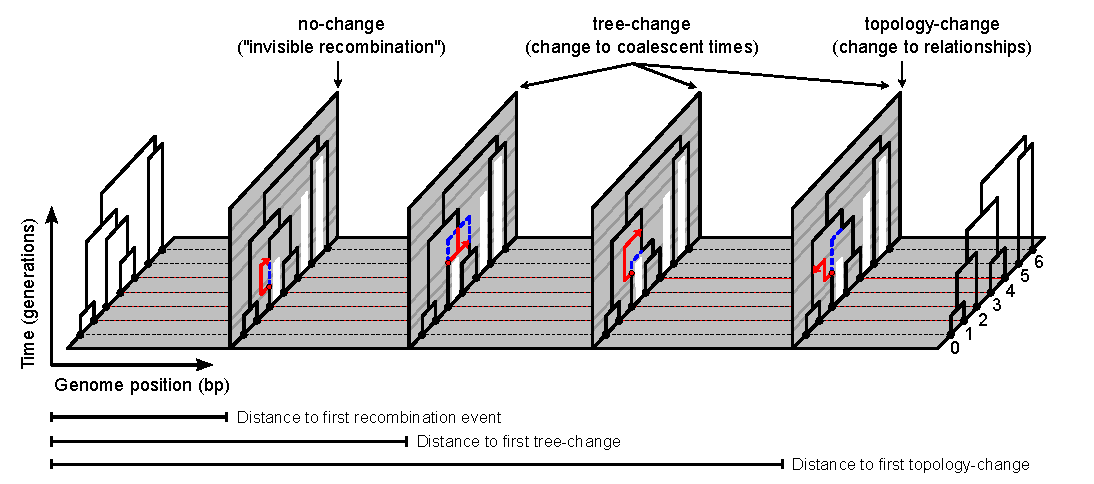
\includegraphics[width=0.99\textwidth]{figures/current/Fig1-recomb-types-on-ARG.pdf}
	\caption{
		% An ancestral recombination graph (ARG) with a demonstration of the coalescent
		% with recombination.
		% The MS-SMC process demonstrated in an ancestral recombination graph (ARG).
		An ancestral recombination graph (ARG)
		is composed of a series of genealogies each spanning non-overlapping 
		intervals of a genome separated by recombination breakpoints. Here, 
		four recombination breakpoints separate \textcolor{red}{interval}
		\textcolor{red}{\sout{the intervals'}}
		start and end positions
		along a small chromosome alignment. The individual genealogies represent the history of a set of 7 samples constrained
		by a 4-tip species tree model
		% 
		\textcolor{red}{(as in Fig.~2).}
		% 
		Recombination events are indicated by vertical panels. Each shows the SMC' process by 
		which a subtree (below the red circle) is detached and then re-coalesces (red arrow)
		with one of the remaining lineages. %, according to the MS-SMC process. 
		The former edge (blue dotted) which existed throughout the interval to the left of a 
		panel is replaced by a new edge (red) through the subsequent interval. 
		Vertical bars 
		(white) represent barriers to coalescence between samples in different species
		tree intervals (MSC model lineages).
		% ancestor is pruned (blue dotted) 
		% and replaced by a new sampled ancestor (red).
		Four categories of recombination events are shown from left to right, representing
		different outcomes based on the lineage with which a detached subtree re-coalesces.
		% : no-change; tree-change resulting in a shortened coalescence time; 
		% tree-change resulting in a lengthened coalescence time; and tree-change 
		% resulting in a different topology. 
		% These can be further consolidated into 
		These are grouped more generally into 
		three \emph{event types}: (1) no-change, (2) tree-change, and (3) topology-change.
		Every recombination event causes either a no-change or tree-change event, whereas
		topology-change events are a subset of possible tree-change events. The expected waiting
		distance until a specific recombination event type occurs can be calculated under 
		the MS-SMC given a starting genealogy, MSC model, and recombination rate.
	% Examples of the four different categories of outcomes from a 
	% recombination event (adapted from \citep{deng_distribution_2021}). 
	% (a) A category 1 event occurs when the dislocated lineage reattaches to the 
	% original lineage. 
	% (b) A category 2 event occurs when a dislocated lineage attaches to its 
	% sibling lineage (the lineage that it originally coalesced with), shortening 
	% both of their branch lengths and extending that of its parental lineage. 
	% (c) A category 3 event occurs when the dislocated lineage attaches to its 
	% parental lineage, lengthening the original lineage and its sibling lineage,
	% and shortening the parental lineage.
	% (d) A category 4 recombination event occurs when the dislocated lineage
	% attaches with any lineage other than itself, its sibling lineage, and its
	% parental lineage. This is the only category of recombination event that
	% changes the topology of the genealogy.
}
\label{fig:ARG-cartoon}
\end{figure}



% Implicit to SMC-based methods is the expectation that recombination occurs at 
% some rate from which the waiting distance between recombination events can be modeled 
% as an exponentially distributed random variable. 
\cite{marjoram2006fast}
described an important extension to the SMC, termed the SMC', for additionally
modeling "invisible" recombination events, in which a detached lineage re-attaches
with its own ancestral lineage prior to the time of that lineage's next coalescent event. 
This leads to no change between the genealogies in two sequential genomic intervals
despite the occurrence of a recombination event between them. The inclusion of
such events has been shown to 
% , such that 
% no change between 
% neighboring genealogies, which has been shown to 
significantly improve inference methods \citep{wilton2015smc}. 
Under the SMC', a detached lineage can thus re-coalesce with an allowable 
ancestral lineage over a continuous range of time, leading to one of 
four possible categorical patterns for the relationship between two
sequential genealogies
% a change 
% relative to the previous genealogy that can be described as one of 
% \hl{four possible categorical} outcomes:
% of possible outcomes of recombination, 
\textcolor{red}{(Fig.~\ref{fig:ARG-cartoon},} Fig.~\ref{fig:figS-recomb-types}): 
(1) no change %between sequential genealogies;
(2) shortening of a coalescent time; (3) lengthening of a coalescent time; 
and (4) %a coalescent event that changes the topology (relationships). 
a change to the genealogical topology (relationships).
These can be grouped more generally into three types: 
"no-change" (category 1), "tree-change" (categories 2-4), and "topology-change"
(category 4). Recently, \citet{deng_distribution_2021} derived a set of 
solutions for the 
\textcolor{red}{\sout{expected} distribution of} 
waiting distances to each of these three types of 
outcomes for a single population with constant effective population size.
% Although all three outcomes, and their associated waiting distances, occur 
% implicitly between sequential genealogies within data generated under the SMC', 
% there was not previously a solution for expectations between events that do 
% not occur sequentially, representing the joint probabilities of multiple events.
% This provides an important advance, for establishing a neutral expectation for 
% turnover 
% in different categorical types of genealogy changes, and for connecting these
% to coalescent model parameters, which may prove useful for future ARG inference 
% tools. 
% 
% 
This provided an important advance by establishing a neutral expectation 
not only for the distance until the next recombination event occurs, 
% 
% but more specifically, for the distance until the next tree-change or 
% topology-change event. Such events leave different detectable signatures 
% in sequence data and extend across larger spatial distances of the genome, 
% thus extending the information content that can be extracted from 
% spatial genealogical patterns.
% 
but more specifically, for the distance until different categorical types
of recombination events occur. Such events leave different detectable 
signatures in sequence data and extend across different spatial distances 
of the genome, thus extending the scale over which information from 
spatial genealogical patterns can be extracted from genomes.
% 
% This provided an important advance by establishing a neutral expectation 
% not only for the distance until the next recombination event occurs, 
% but more specifically, for the distance between different categorical types
% of recombination events that leave different detectable signatures in 
% sequence data. Because such patterns extend over greater spatial distances
% of the genome, they extend the distance over which we can make 
% statistical predictions about spatial genealogical patterns.
% 
% Because they extend over greater spatial distances, information
% from tree-change and topology-change events 
% methods based
% on the detection of
% such patterns can extend the information content of spatial genealogical data.
% until the next tree-change or 
% topology-change event. 
% % Such events leave 
% These different types of recombination events leave different
% detectable signatures in sequence data, and extend across larger 
% spatial distances of the genome, thus extending the information content
% that can be extracted from spatial genealogical patterns.
% than that to the next generic recombination event. 
% This provides an important advance by establishing a neutral expectation 
% not only for the distance until any generic recombination event occurs, 
% but more specifically, for % the different expectations for 
% % for 
% different types 
% of events that leave different detectable signatures in the genome.
% not
% only for any generic recombination events to occur, but for different types 
% of events that leave different detectable signatures in the genome.
% ,which may prove useful for the development of future SMC'-based tools.
% in genealogical topologies, and for connecting coalescent model parameters to these
% outcomes, which may prove useful for future advances in ARG inference. 

% \citep{deng_distribution_2021} recently 
% Their solution assumes a single population with constant effective population size, 
% but nevertheless ... 
% Their solutions 


% recently described a partitioning of different possible outcomes of recombination 
% events into three categories: (1) "no effect", which do not change the genealogy; 
% (2) "tree changes", which affect only coalescent times (edge lengths); and 
% (3) "topology changes", which affect the genealogical relationships.

% the expected waiting distances between
% recombination events, describing different rates for three categorical
% types of recombination events that can occur (Fig.~\ref{fig:fig2}). 
% % 
% This includes recombination events that: (1) have no affect on the 
% genealogical tree; (2) cause "tree changes" (i.e. that they 
% affect either the branch lengths or the topology of the genealogical tree, 
% as in any of categories 2, 3, and 4), and those that cause "topology changes" 
% (only category 4) (\textbf{Figure 1}).


% \citet{deng_distribution_2021} derived an approximate solution for the 
% distribution of waiting distances between sequential genealogies in an ARG. 
% This involved extending the simple expectation for the expected waiting distance
% between *any* recombination event, and partitioning the results into categories
% of different possible outcomes (Fig.~\ref{fig:fig2}). 

% , some of which result in changes to 
% the genealogy, and others of which do not. 
% This represents a major advance. Although 
% The expected waiting distance between any recombination event can be modeled as
% a simple simply described by an exponential distribution}, 
 % under the SMC’ 

% an extension of the SMC that includes "invisible" recombination
% events that result in no change between neighboring genealogical trees. 
% \hl{was known previously}, 
% \citet{deng_distribution_2021} 


Here, 
\textcolor{red}{
\sout{we extend the methods of \mbox{\citet{deng_distribution_2021}} to an MSC framework 
to estimate the expected waiting distances between different types of}
we extend the theory of \citet{deng_distribution_2021} to an MSC framework
to derive the distribution of the waiting distance until different types of
} 
genealogy changes 
\textcolor{red}{occur} 
under a parameterized species tree model.
The waiting distances between recombination events that cause topology-change 
may be of greatest interest, as they leave the most detectable signatures 
in sequence data and are relevant to expected gene tree distributions that form
an important component of many MSC-based methods \citep{
degnan2009gene, baum_concordance_2007, knowles_estimating_2011}.
% Just like for single-population models, 
% the waiting distance until a topology-change event in this framework can include multiple
% intervening recombination events of the no-change or tree-change type
The waiting distance between topology-change events may include multiple
intervening recombination events of the no-change or tree-change type
\textcolor{red}{(Fig.~\ref{fig:ARG-cartoon}).}
The relative occurrence of events that do not result in topology 
changes can be especially high in small sample sizes \citep{wilton2015smc}, 
which are common in MSC-type datasets in which samples are partitioned 
among species tree intervals. 
% The partitioning of 
% recombination events that of categories 1-3 occur 
% disproportionately often in small sample sizes \citep{wilton2015smc}, 
% which are especially common in MSC-type datasets since
% samples are partitioned among species tree intervals. 
Since the partitioning of 
coalescent events among species tree intervals is expected to constrain 
the types of recombination events that will be observed, the
distributions of waiting distances between different types of 
genealogy changes should be highly dependent on, and thus informative about, 
the species tree model. We refer to the general framework of embedding the 
SMC' in an MSC model as the MS-SMC.


% The relative frequency
% of different event types is therefore expected to be contingent on parameters
% of the species tree. 

% Recombination events of type 4 are of greatest interest
% % the most inherently interesting 
% for most applications,
% % because s
% as they leave the most detectable signal in sequence data.
% % since they will produce the most obvious signal in the sequence data. 
% However, events of types 1-3 occur disproportionately often in small sample 
% sizes \citep{wilton2015smc}, which are especially common in MSC-based studies, 
% where genealogies are embedded within a species tree, such that fewer samples 
% typically represent each lineage. But the
% relative frequency of the different events is contingent upon the Ne values of the
% species tree branches and on the species divergence times. In other words, the 
% partitioning of coalescence events among lineages of the species tree topology is
% expected to constrain the types of recombination events that are more likely to be
% observed. This results in distributions of waiting distances between genealogical
% changes being highly dependent upon parameters of the species tree model. 

% With this in mind, we extend the method of \citet{deng_distribution_2021} to the MSC
% to predict the expected waiting distances between genealogy changes under a 
% parameterized species tree model. This new solution is important for establishing an 
% expectation for the neutral rate of genealogy turnover under different species tree 
% parameterizations. It may also have applications for ARG inference under complex 
% demographic models \citep[e.g.,][]{hubisz2020mapping}, potentially serving as a 
% component of a likelihood function for inferring species trees from linked 
% genealogies -- a future theoretical goal.

% MS-SMC: multispecies sequentially markovian coalescent
% SM-MSC: sequentially markovian multispecies coalescent

%Solutions exist for simulating genomes under the coalescent with recombination \citet{ipcoal, kelleher, hudson}. In particular, \emph{msprime} is a powerful and flexible tool for simulating ancestral recombination graphs for many samples under user-defined demographic scenarios. \emph{ipcoal} is an extension of msprime that accepts multispecies coalescent parameters. 

%Phylogenetic methods sampling regions throughout the genome have increasingly adopted the multispecies coalescent model to incorporate variation in regions due to incomplete lineage sorting. Applications of the multispecies coalescent in phylogenetic inference aim to avoid known bias under which, in certain circumstances, phylogenies inferred from concatenated data might converge on a tree that is not the species tree. One challenge of applying the multispecies coalescent for species tree inference is properly defining the breakpoints for loci used in the analysis. Often this is done arbitrarily: researchers ensure that loci are long enough to infer reliable gene trees, and that there are enough inferred gene trees to infer a robust species tree. However, there has been some debate in the literature over the effects of locus length on species tree inference. Specifically,  

%Another way in which the ancestral recombination graph is relevant to phylogeneticists is for local inference...

%Recently, \citet{deng_distribution_2021} provided a solution for the distribution of waiting times to genealogical changes under the SMC', a popular model for simulating ancestral recombination graphs. However, their solution is constrained to a single population of constant effective population size.

%Establishing the predicted length of different topologies along the chromosome is important for inference of local genealogies in population genetics, which can be used for inference of selection, demographic changes, and introgression. It is also important in multispecies coalescent methods in phylogenetics, which often rely on inference of gene trees.


% springer + gatesy

% inference, argweaver-D



%%%%%%%%%%%%%%%%%%%%%%%%%%%%%%%%%%%%%%%%%%%%%%%%%%%%%%%%%%%%%%%%%%%%%%%%%%%
%%%%%%%%%%%%%%%%%%%%%%%%%%%%%%%%%%%%%%%%%%%%%%%%%%%%%%%%%%%%%%%%%%%%%%%%%%%
%%%%%%%%%%%%%%%%%%%%%%%%%%%%%%%%%%%%%%%%%%%%%%%%%%%%%%%%%%%%%%%%%%%%%%%%%%%
%%%%%%%%%%%%%%%%%%%%%%%%%%%%%%%%%%%%%%%%%%%%%%%%%%%%%%%%%%%%%%%%%%%%%%%%%%%
%%%%%%%%%%%%%%%%%%%%%%%%%%%%%%%%%%%%%%%%%%%%%%%%%%%%%%%%%%%%%%%%%%%%%%%%%%%
%%%%%%%%%%%%%%%%%%%%%%%%%%%%%%%%%%%%%%%%%%%%%%%%%%%%%%%%%%%%%%%%%%%%%%%%%%%
%%%%%%%%%%%%%%%%%%%%%%%%%%%%%%%%%%%%%%%%%%%%%%%%%%%%%%%%%%%%%%%%%%%%%%%%%%%
%%%%%%%%%%%%%%%%%%%%%%%%%%%%%%%%%%%%%%%%%%%%%%%%%%%%%%%%%%%%%%%%%%%%%%%%%%%
%%%%%%%%%%%%%%%%%%%%%%%%%%%%%%%%%%%%%%%%%%%%%%%%%%%%%%%%%%%%%%%%%%%%%%%%%%%
%%%%%%%%%%%%%%%%%%%%%%%%%%%%%%%%%%%%%%%%%%%%%%%%%%%%%%%%%%%%%%%%%%%%%%%%%%%






\section{Approach}
\subsection{Comparison to Deng \emph{et al.} (2021)} %\citet{deng_distribution_2021}}

Our approach is a generalization of the \citet{deng_distribution_2021} derivation 
of waiting distances to genealogy changes for a single population of constant size. 
We modified the single-population model to (1) include barriers to coalescence imposed
by a species tree topology, and (2) integrate over changing coalescence rates along
paths through multiple species tree intervals with different effective population 
sizes. 
\textcolor{red}{
\sout{
In addition, we have implemented a novel likelihood framework for inferring 
parameters of an MSC model from observed waiting distances between genealogies.
}
In addition, we introduce a novel application of our MS-SMC model, utilizing
a likelihood-based framework to estimate MSC model parameters from the waiting
distances between tree-change and topology-change events.
}
% likelihood implementation that makes
% use of the probability density of waiting distances to fit species tree
% parameters given an observed ARG, and to infer ARGs given a parameterized
% species tree.
% }

% \textcolor{red}{
% - more info?
% - likelihood framework?
% We demonstrate that applying the MS-SMC model to structured population data 
% can extract more information from the spatial
% distribution of genealogies 
% present in a single population
% ...
% of a single population model to multiple structured population
% models to demonstrate 
% We demonstrate how this extension allows for the development of a 
% new framework for calculating the likelihood of an ARG
% ...}
% We have intentionally reproduced our equations in a similar structure and using
% many of the same variable names as in \citet{deng_distribution_2021}.
% to highlight the changes we made to generalize their solution.


\subsection{MSC model description}
% We assume a species tree model with divergence times in units of generations and 
Given an MSC model ($\mathcal{S}$) composed of a species tree topology with divergence
times ($W$) in units of generations and constant diploid effective population 
sizes ($N_e$) assigned to each branch, an embedded genealogy ($\mathcal{G}$) for 
any number of sampled gene copies ($k$) can be generated
by randomly sampling coalescent times at which to join two samples into a 
common ancestor, starting from samples at the present in each interval.
% 
% . This is accomplished by randomly sampling coalescent times 
% at which to join two samples into a common ancestor, 
% starting from samples at the present in each interval. 
% 
% 'in each interval' is to be clear that we move piecewise through the MSC model.
% 
Following \citet{kingman1982coalescent}, the probability of a 
coalescent event one generation in the past (reducing the 
number of samples from $k$ to $k$-1) %in a single population
is given by equation 1. From this, we can model the expected 
waiting time ($\mathbb{E}[t_k]$) until the next coalescence event as an 
exponentially distributed random variable with rate parameter $\lambda_k$:

\begin{equation}
\begin{aligned}
	&\lambda_k = \mathbb{P}(\text{coal~event~} | N_e,k) = \frac{k(k-1)}{2N_e}
	\\
	&~~and:
	\\[0.15cm]
	&\mathbb{E}[t_k] = 1 / \lambda_k
	\\[0.15cm]	
\end{aligned}
\end{equation}

\noindent In a single population model
with constant $N_e$ the expected waiting time between coalescent events 
increases monotonically after each coalescent event, since the number of
% with constant $N_e$, the expected waiting time between coalescent events 
% increases monotonically after each coalescent event. This is because the number of 
remaining samples always decreases. In an MSC model, 
however, the expected waiting time between coalescence events can increase or 
decrease through time, as the transition from one population interval to another 
can be associated with a different $N_e$ value and an increase in the number 
of samples.
% to the next can be 
% associated with different N$_b$, and because the merging of samples from 
% number of samples increases
% in ancestral population intervals when descendant branch intervals are merged.


% 1. G probabilities can be calculated.
% 2. The probability of a G is calculated from its coalescent times.
% 3. 
Based on this generative framework for sampling genealogies 
\textcolor{red}{
under a demographic model, 
the probabilities of observed genealogies can also be calculated under 
a demographic model.
% 
The probability of a genealogy embedded in a single population model is
the product of the probability densities of each waiting time between 
coalescent events \citep{kingman1982coalescent}. 
% 
The process is similar for a genealogy embedded in a species tree model, but
requires evaluating the probabilities of coalescent waiting times within each
species tree interval separately -- 
including the probability that all gene copies do not coalesce before the 
end of the interval \citep{rannala2003bayes}.
% 
A key feature of this framework is that for each coalescent interval 
with $k$ gene copies and effective population size $N_e$, we can 
calculate the coalescent rate ($\lambda_k$) and use the exponential probability
density function (Equation 2) to evaluate the likelihood of the 
demographic model parameters based on the distributions of coalescent 
times in one or more genealogies.
% 
% The  of model parameters, such as $N_e$ for a single population model, 
% or multiple $N_e$ and $W$ parameters for a species tree model, that jointly
% maximize the likelihood represent the best fit to the data.
}

% waiting probabilities of waiting 

% , whereas
% the probability of a genealogy under a species tree model requires 
% calculating the probability of coalescent events within each species
% tree interval separately, as well as the probability that gene copies
% do not coalesce before the end of an interval
% \citep{kingman1982coalescent, rannala2003bayes}.
% % 
% Because the waiting times between coalescent events are exponentially
% distributed, likelihood-based methods have been developed for estimating
% demographic model parameters, such as $N_e$ and $W$, by evaluating 
% the probabilities of genealogies calculated from the distributions of
% their coalescent times \citep{kingman1982coalescent, rannala2003bayes}.
% % 
% A key feature is that for each interval between coalescent events 
% we can calculate the coalescent rate parameter ($\lambda_k$) based 
% on the current $k$ and $N_e$, and use the the exponential probability
% density function (Equation 2) to evaluate the likelihood of the model
% parameters given the distribution of waiting times.
% }
% For a genealogy embedded in a species tree this process is similar, 
% but requires evaluating the probability of each coalescent event within
% each parameterized species tree interval, as well as the probability 
% that gene copies do not coalesce in an interval
% \citep{rannala2003bayes}.
% 
%  given the (lamb) to calculate the 
% likelihood of 
% observed waiting times between coalescent events (t k ) in
% each population interval from an the exponential probability density function:
% The waiting times between coalescent events
% % 
% In a single population model with constant $N_e$, the genealogy 
% probability is calculated as the product of the probabilities of
% each waiting distance between coalescent events. 

% probability of
% a genealogy is the product of the probabilities of each coalescent event
% \citep{kingman1982coalescent}. For a species tree this process is
% similar, but involves calculating the probability of coalescent events
% within each species tree interval separately, in addition to the probability
% that they do not coalesce before the end of an interval
% \citep{rannala2003bayes,mirarab_multispecies_2021}.
% A likelihood function can then be used find the model parameters that
% maximize the likelihood, to estimate $N_e$ for a single population model,
% or jointly estimate $N_e$ and $W$ parameters of a species tree model.
% 
% \textcolor{red}{
% \sout{likelihood solutions}
% likelihood-based solutions
% } 
% have been developed to fit coalescent model parameters, such as 
% $N_e$ in single population models \citep{kingman1982coalescent},
% or multiple $N_e$ and $W$ parameters in MSC models \citep{rannala2003bayes,mirarab_multispecies_2021}, 
% based on inferred coalescence times. 
% In the latter framework, each species tree branch interval is treated independently, 
% such that the likelihood of a genealogy embedding is calculated from the joint
% probability of observing each distribution of coalescent waiting times within
% each species tree branch interval. A key feature of these equations is that 
% when $k$ lineages are present, we can use the coalescent rate parameters 
% ($\lambda_k$)
% % \hl{the inverse of} equation 1 as a rate parameter ($\lambda$)
% to calculate the \textcolor{red}{probability}\sout{likelihood}}
% of observed waiting times between coalescent 
% events ($t_k$) in each population interval from 
% \textcolor{red}{\sout{an} the}
% exponential probability density function:
% for the expected rate
% of coalescence
% between when $k$ and $k$ - 1 lineages exist. 
%  and thus the probability of 
% when Using the expected time between coalescence
% events when $k$ lineages are present (equation 1) as a rate parameter, the 
% likelihood of an observed waiting time can be calculated from an exponential 
% probability density. 
	
\begin{equation}
	% \mathcal{P}(t_k|\lambda) = \lambda e^{-\lambda t_k} 
	f(t_k; \lambda_k) = \lambda_k e^{-\lambda_k t_k}
\end{equation}


% In each species tree interval this is repeated for each interval between 
% observed coalescent events.

% The probability of a particular genealogical topology among a set of coalesced
% samples in an interval. The probability a particular pair of lineages coalesce
% is 1 ( kchoose2) = (2 / (j * (j - 1))), where j=m, n, n+1. [Describe m and n as
% the start and end of intervals.]

% \begin{equation}
% 	\mathbb{P}(t_k | N_e) = 
% 		\frac{1}{2N_e} 
% 		\exp \bigg\{-\frac{k(k-1)}{4N_e} t_k \bigg\} \times 
% 		\exp \bigg\{-\frac{n(n-1)}{4N_e} (\tau - (t_m + t_{m-1} + \text{...} + t_{m+1})) \bigg\}
% \end{equation}

% Similarly, the likelihood of observing a set of coalescent
% times on a genealogy embedded in a species tree can be calculated from the
% joint probability of its observed coalescence times within each interval
% \citep{rannala2003bayes}, treating intervals independently. 
% Thus, the genealogy (G) in Figure 1 can be calculated as
% ...

% Generating unlinked genealogical trees under the MSC is straightforward: Coalescent events between samples can only happen after (moving backward in time) coalescence of the species that contain them, and the coalescent rate in each part of the tree is dependent on both the number of genealogical lineages that can coalesce in that section and on the effective population size in that section.

\subsection{MS-SMC model description and notation}

% Under the single-population SMC' 
% considered by \citet{deng_distribution_2021}, the 
Under the SMC' model, sampling of a linked genealogy requires considering not only 
%a species tree and its parameters, 
demographic model parameters, 
as we did above, but also an existing genealogy -- it is a method 
for sampling the next genealogy conditional on the previously observed one. 
If we define the previous genealogy as $\mathcal{G}$, and the sum of its edge lengths 
as $L(\mathcal{G})$, then under the assumption of a constant recombination rate through time,
a recombination break point can be uniformly sampled from $L(\mathcal{G})$ to occur with 
equal probability anywhere on $\mathcal{G}$. 
% on any branch.
A recombination event creates a bisection on a branch, separating a subtree 
below the cut from the rest of the genealogy 
\textcolor{red}{
(Fig.~\ref{fig:ARG-cartoon}, Fig.~\ref{fig:figS-recomb-types}).
}
% (Fig.~\ref{fig:fig2}). 
The subtree must then re-coalesce 
with an edge on the genealogy from which it was detached at a time
above the recombination event.
%in the to connect with one of the edges of %remaining edges on 
% the genealogy at a time above the recombination event. 
The waiting time until 
this re-coalescence event occurs is sampled stochastically 
\textcolor{red}{
\sout{with an expectation determined by the number of samples and
the coalescent rate, similar to equation 1.
}
using equation (1), where the expectation is determined by the 
number of samples and the effective population size.
} % coalescent rate.}
% the expected waiting time as until re-coalescence the 
% same as described above (equations 1 and 2).

In a single population model with constant $N_e$, the expected waiting time until 
re-coalescence increases monotonically with each coalescence event 
backwards in time, since each event decreases $k$.
% (e.g., Fig.~1B). 
Once again, the MSC model differs from this: 
coalescent events similarly decrease $k$, but the merging of 
species tree branches into ancestral intervals increases $k$, and $N_e$ 
can also vary among species tree intervals. 
Thus, the probability that a detached subtree re-coalesces to the genealogy 
can vary through time along its path of possible reconnection points through 
different species tree intervals.
% 
\textcolor{red}{\sout{(Fig.~3)}}
% 
To calculate these probabilities, a species tree and genealogy can be decomposed into a 
series of relevant intervals between events that change rates of coalescence,
% , including within species tree intervals, 
which we refer to as the genealogy embedding table 
\textcolor{red}{
(Fig.~\ref{fig:embedding-table}).
\sout{(Table~1).}
}
% 
From this table it is possible to calculate the probabilities of different
recombination event type outcomes and, consequently, to model the expected 
waiting distances until specific recombination event types occur. 

% Using this information on the rate of coalescence within each genealogy
% embedding interval, it is then possible to model the probability that a
% detached lineage will re-coalesce within any specific interval. From this, 
% it is then possible to calculate probabilities of different recombination event types which 
% are a
% Our goal ... The goal of the MS... To model the probabilities of different
% genealogy change events we must model the probability that a detached lineage
% will re-coalesce with any allowed ancestral lineage while constrained by the
% MSC model. This requires integrating over the coalescence rates which can 
% vary among intervals of the species tree model.


% PREVIOUS TABLE WAS REPLACED HERE BY A FIGURE THAT INCLUDES AN IMAGE AND TABLE
\begin{figure}[t]
	\centering
	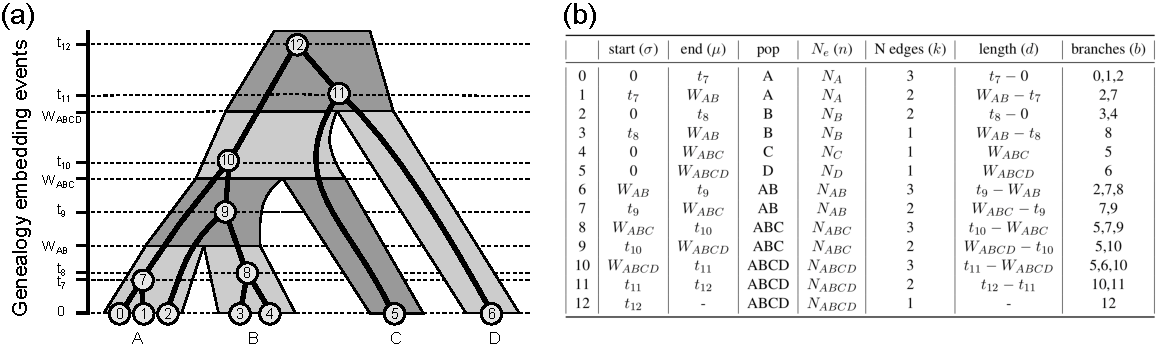
\includegraphics[width=0.99\textwidth]{figures/current/Fig2-embedding-table.pdf}
	\caption{
		An example genealogy embedded in a species tree and the corresponding
		embedding table used for MS-SMC calculations. 
		(a) A four tip species tree is composed of seven discrete population
		intervals separated by speciation events ($W_x$), each of which can be
		further dissected by coalescent events ($t_x$).
		(b) The probability of coalescence is constant within each discrete
		interval and is scaled by the number of lineages ($k$), the effective 
		population size ($n$), and the interval length ($d$).
		% present ($k$) and the effective population size ($N_e$). 
		Under the MS-SMC, the probability that a detached lineage will re-coalesce
		on a specific branch of the genealogy (e.g., branch 7) is calculated using
		the piecewise constant probabilities from each discrete interval spanning
		that branch (e.g., rows 1, 6, 7, and 8 in the embedding table).
	}
\label{fig:embedding-table}
\end{figure}

% \begin{table}[t]
% \centering
% \caption{
% 	A genealogy embedding table for the genealogy and species tree in Figure 1. 
% 	The probability of coalescence is constant within each discrete interval 
% 	and is scaled by the number of lineages ($k$), the effective population size ($n$), 
% 	and the interval length ($d$).
% 	% present ($k$) and the effective population size ($N_e$). 
% 	Under the MS-SMC, the probability that a detached lineage will re-coalesce
% 	on a specific branch of the genealogy (e.g., branch 7 from Figure~\ref{fig:fig1})
% 	is calculated using the piecewise constant probabilities from each 
% 	discrete interval spanning that branch (e.g., rows 1, 6, 7, and 8).
% }
% \begin{tabular}[t]{ |c|c|c|c|c|c|c|c|c| }
% 	\toprule
% 	 % & start ($t_i^l$)  & end ($t_i^u$) 
% 	 & start ($\sigma$)  & end ($\mu$)  & pop & $N_e$ ($n$)  & N edges ($k$) & length ($d$) & branches ($b$) \\
% 	\midrule
% 	0 & 0          & $t_7$      & A   & $N_A$     & 3 &  $t_7$ $-$ 0            & 0,1,2 \\
% 	1 & $t_7$      & $W_{AB}$   & A   & $N_A$     & 2 &  $W_{AB}$ $-$ $t_7$     & 2,7   \\	
% 	2 & 0          & $t_8$      & B   & $N_B$     & 2 &  $t_8$ $-$ 0            & 3,4   \\ 
% 	3 & $t_8$      & $W_{AB}$   & B   & $N_B$     & 1 &  $W_{AB}$ $-$ $t_8$     & 8     \\
% 	4 & 0          & $W_{ABC}$  & C   & $N_C$     & 1 &  $W_{ABC}$              & 5     \\
% 	5 & 0          & $W_{ABCD}$ & D   & $N_D$     & 1 &  $W_{ABCD}$             & 6     \\
% 	% 
% 	6 & $W_{AB}$   & $t_9$      & AB  & $N_{AB}$  & 3 &  $t_9$ $-$ $W_{AB}$     & 2,7,8 \\
% 	7 & $t_9$      & $W_{ABC}$  & AB  & $N_{AB}$  & 2 &  $W_{ABC}$ $-$ $t_9$    & 7,9   \\
% 	% 
% 	8 & $W_{ABC}$  & $t_{10}$   & ABC & $N_{ABC}$ & 3 &  $t_{10}$ $-$ $W_{ABC}$  & 5,7,9  \\
% 	9 & $t_{10}$   & $W_{ABCD}$ & ABC & $N_{ABC}$ & 2 &  $W_{ABCD}$ $-$ $t_{10}$ & 5,10   \\
% 	%
% 	10 & $W_{ABCD}$ & $t_{11}$  & ABCD & $N_{ABCD}$ & 3 & $t_{11}$ $-$ $W_{ABCD}$ & 5,6,10 \\
% 	11 & $t_{11}$  & $t_{12}$   & ABCD & $N_{ABCD}$ & 2 & $t_{12}$ $-$ $t_{11}$   & 10,11 \\
% 	12 & $t_{12}$  & -          & ABCD & $N_{ABCD}$ & 1 & -                       & 12    \\	
% 	\bottomrule
% \end{tabular}
% \label{tab:table-1} 
% \end{table}

Each interval of the genealogy embedding table contains a constant number
of genealogy branches ($k_i$) and a constant effective population size 
($n_i$) such that the rate of coalescence is also constant.
We define a number of additional variables related to this table. 
The length of each interval is $d_i$, and its lower and upper bounds 
are $\sigma_i$ and $\mu_i$, respectively. Similarly, the lower and upper 
bounds of a genealogy branch ($b$) are defined as $t_b^l$ and $t_b^u$, 
respectively. 
% Each interval has a constant 
% number of genealogy branches $k_i$, and effective population size $n_i$.
An indexing variable, $\mathcal{I}_b$, is defined as the
ordered set of intervals that are spanned by a specific branch
of an embedded genealogy. As an example, consider 
\textcolor{red}{genealogy}
branch 7 from 
% 
Fig.~\ref{fig:embedding-table}a.
% 
\textcolor{red}{\sout{Fig.~3}}
% Fig.~\ref{fig:edge-probabilities}. 
This branch spans four intervals, 
labeled as rows 1, 6, 7, and 8 in
the associated genealogy embedding table
(Fig.~\ref{fig:embedding-table}b),
% 
\textcolor{red}{\sout{Table~1}}
% Table~\ref{tab:table-1}, 
% 
and so $\mathcal{I}_7$ = \{1,6,7,8\}. As we will
demonstrate below, this and related indexing variables will be
used to calculate the probabilities of re-coalescence in different
intervals, and on different branches, based on their rates of 
coalescence.
A summary of all variables in our notation is available in 
table~\ref{tab:table-notation}. 

% To better understand the relationship between the MS-SMC and the genealogy
% embedding table, consider a specific branch ($b$) from Fig.~\ref{fig:fig1}. 
% Branch 7 on the genealogy spans four relevant intervals, 
% labeled as rows 1, 6, 7, and 8 in Table~\ref{tab:table-1}.
% This ordered set is defined as $\mathcal{I}_b$, such that, for example, 
% $\mathcal{I}_7$ = \{1,6,7,8\}. 
% Several additional indexing variables are described below;
% a summary of all variables is available in table~\ref{tab:table-notation}). 

% The coalescent rate within each interval can be calculated from its
% \hl{diploid} effective population size ($n_i$) and number of samples 
% present ($a_i$). 
% The lower and upper bounds of each interval are defined as 
% $\sigma_i$ and $\mu_i$, respectively, and its length as $d_i$. 
% Similarly, the lower and upper bounds of each branch are defined 
% as $t_b^l$ and $t_b^u$, respectively. Each interval has a constant 
% number of genealogy branches $k_i$, and effective population size $n_i$.
% This is used in the equations below as an
% index to iterate over the ordered sequence of intervals on a branch. 
% By iterating over all $i$ intervals from 0 to $\mathcal{I}_b - 1$ 
% different rates can be applied to different intervals over the length 
% of a branch.
% (this can be found by searching for the branch label in the \emph{branches} 
% column of the table). 
% We record the number 
% of intervals in which a branch is present as $\mathcal{I}_b$, such that,
% for example, $\mathcal{I}_7$=4. We use this indexing variable to iterate
% over the ordered sequence of intervals on a branch. 
% over the lengths of each interval on a branch. 
% The coalescent rate within each genealogy embedding interval of the
% table is calculated from the \hl{diploid} effective population size ($n_i$) 
% and number of samples present ($a_i$).
% to the end of the last interval $\sigma_{\mathcal{I}_{b+1}}$.
% For this branch, we are interested in defining intervals where 
% coalescent rate parameters change, 
% which involves identifying coalescent events that occur in the same species
% tree intervals as this branch, as well as events where this branch 
% transitions from one species tree interval to the next.
% To do so, we must identify times at which there are relevant coalescent events 
% between other lineages in the same population, or at which there are relevant 
% species merging events. 
% This involves examining the genealogical tree as it is 
% embedded within the species tree. With the genealogy embedding table, we can 
% In the genealogy embedding table we can then query the "branch" column to
% isolate intervals involving branch 7. This corresponds to rows 1, 6, 7, and 8, 
% such that the number of intervals on branch 7 ($\mathcal{I}_b$) is four. 
% The time of the start of each interval ($i$) is $\sigma_i$. 
% \hl{An integer index ($\mathcal{I}$) stores the number of intervals that 
% each branch occurs in, such that enumerating over the range
% of $\mathcal{I}_b$ visits each interval in order along 
% genealogy branch $b$.} 
% easily isolate the intervals specific to edge 7 by querying the "branches" 
% column of the table and extracting the rows where this column contains our 
% focal edge (for edge 7, these are rows 1, 6, 7, and 8). 
% The number of rows is equal to the 
% The number of rows 
% we extract (in this case, 4) is equal to the number of intervals in the edge 
% ($\mathcal{I}_b$). If we retain the relative order of the rows and re-index them from 
% $0$ to $\mathcal{I}_b-1$, the information in the columns (e.g. $n_i$, $a_i$) is easily
% adapted for use in the equations presented below. 
% Each branch of $\mathcal{G}$ spans one or more intervals
% from which a lower and upper (min, max) bound for that branch can also be 
% extracted ($t_b^l$ and $t_b^u$, respectively). 
% Later, we describe equations that require information about how genealogy branches are 
% related (e.g., parent-child or siblings), which can also be extracted from $\mathcal{G}$
% and represented as a table. 
% Some additional indexing variables are also described below;
% a summary of all variables is available in table~\ref{tab:table-notation}). 

% This and the genealogy embedding table include all
% relevant parameters for the equations below. 
 % \hl{(e.g., Table~S1).}
% . For example, 
% edge 2 from Fig.~\ref{fig:fig1} and Table~\ref{tab:table-1} overlaps with 
% three intervals, such that $\mathcal{I}_2$ = 3.
% \hl{From this gene tree embedding we also define 
% the set $\mathcal{I}$ that includes the indices of all intervals in the table. 
% And we define an indexing variable $I_b$ for each branch ($b$) in $\mathcal{G}$ that
% returns a vector of ordered intervals ($i \in \mathcal{I}$) that overlap with 
% a specific gene tree branch.}
% For example, edge 2 from Fig.~\ref{fig:fig1} and Table~\ref{tab:table-1} overlaps with 
% three intervals, such that $I_2$ = (0, 1, 6). 
% These variables, and the genealogy embedding table, 
% together include all relevant parameters for the derivations below. 



% To summarize, the genealogy embedding table is simply a set containing all 
% unique intervals (and their properties) over all edges in the genealogy, 
% and it maps those intervals to the genealogy edges to which they belong. 
% This allows us to easily query relevant intervals for any edge of the 
% genealogical tree. For extracting relationships among branches (e.g. parent,
% sibling, as required for the topology cahnge equations), we can reference a 
% separate table specific to the structure of the genealogical tree only (see 
% Appendix, Table 2).
% , and are also summarized in the Appendix.

%\hl{needs updates to figure out how table can align with existing variables names.
%Additional table with final info could be supplement. Includes I, sister index, parent index...}

% Unlike in the single-population SMC', the intervals in the multispecies model
% are branch-specific. For example, the breakpoint $\sigma_{D1}$ in Figure 2c  
% corresponds to the species tree coalescence of species C and species D. This 
% increases the number of lineages available for the D lineage to coalesce with 
% (from 1 -- itself -- to 2) and might also change the effective population size.
% However, this breakpoint does not appear in Figure 2d since the lineage in species
% E is not able to coalesce with lineages from species C or D until $\sigma_{E1}$,
% when E coalesces with the ancestor of C and D in the species tree.




% In the MS-SMC, we specify a model with piecewise-constant coalescence rates. 
% However, intervals under the MSC adaptation are bounded not just by coalescence
% events in the \emph{genealogy} tree (decreasing the number of available lineages for 
% coalescence), but also by relevant coalescences in the \emph{species} tree. Species 
% coalesence events increase the number of genealogical lineages available for 
% coalescence, and they also can correspond to changes in effective population 
% size (\textbf{Figure 2}). 

% Having described our model, we also adopt the following notation:

% \begin{itemize}
%   \item $\mathcal{I}_b$: index of an interval on genealogy branch $b$. A genealogy 
%   branch is split into discrete intervals corresponding to points along its length 
%   at which either the species tree interval changes, or the number of samples $k$ with
%   which it can coalesce changes.
%   \item $t^u_b$: the height, in generations, of the upper bound of genealogy branch $b$.
%   \item $t^l_b$: the height, in generations, of the lower bound of genealogy branch $b$.
%   \item $\mathcal{T}$: the genealogical tree
%   \item $\mathcal{S}$: the species tree
%   \item $\mathcal{N}$: the number of tips in the species tree
%   \item $L(\mathcal{T})$: the total genealogical tree length, in generations
%   \item All summations where the stopping value is less than the starting value are equal to zero.
% \end{itemize}

% Several values are indicated only on one branch at a time, and thus we do not include 
% an underscore to indicate which branch. These are:
% \begin{itemize}
%   \item $\sigma_i$: the length, in generations, of the lower bound of interval $i$ on branch $b$.
%   \item $n_i$: the effective population size of species tree interval index $i$.
%   \item $a_i$: the number of available lineages to coalesce with in the genealogy interval with index $i$.
%   \item $T_i$: the length, in generations, of species tree interval with index $i$.
% \end{itemize}


\subsection{Deriving probabilities of genealogy changes in the MS-SMC}
A recombination event occurring on $\mathcal{G}$ can result 
in three types of outcomes (Fig.~\ref{fig:ARG-cartoon}).
Of these, there is a zero-sum relationship between a no-change and 
tree-change event, such that one or the other must occur.
% one or the other must always occur.
% , resulting in either 
% no change to the genealogy, a change only to its branch lengths, 
% or a change to its topology. 
Therefore, as a first step towards describing probability statements 
for each of these event types, we focus first on deriving the 
probability of a no-change event 
(also termed a tree-unchanged event; Fig.~\ref{fig:fig3}a),
which is the simplest outcome. Then, from the law of total probability, 
we also have a result for the probability of recombination resulting in 
a tree-change event. 
% From this, we can then calculate the probability of a tree-change
% by the law of total probability. 
% Therefore, our first step in deriving probability statements for
% Our first step in deriving probability statements for
% these different outcomes is to calculate the probability of a no-change event. 
Finally, to calculate the probability of a topology-change event, 
we first derive a statement for the probability of a topology-unchanged event
(Fig.~\ref{fig:fig3}d), which is the union of a no-change event and
a subset of tree-change events,
where the detached lineage is restricted according to which ancestral lineages 
it can re-coalesce with. 
Full detailed derivations of all solutions below are available in the 
Appendix of the Supplementary Materials.
% we calculate the probability of topology-change as a subset of
% the probability of a tree-change, in which we restrict which branches the
% detached lineage can re-coalesce with.
% events. 
% probabilities 
% of events that 
% fall into the other categories.
% In category 1, there is no change to the genealogy. In categories 2 and 3 only
% a the branch lengths of the genealogical tree change while the topology remains
% the same. In category 4, the topology of the resulting tree is different from the 
% original tree. For simplicity, we will refer to changes that affect only branch
% lengths (categories 2-3) as those that change \emph{the tree}, and category 4 as 
% those that change \emph{the topology}.
% Our first steps are to calculate the probability of a recombination event in
% category 1, where the new genealogical tree is identical to the previous tree. The 
% law of total probability then allows us to use the inverse probability to calculate
% a waiting distance to a change that falls into any of categories 2, 3, or 4. 


\subsubsection{Probability of a no-change event}
% \subsubsection{Probability that a recombination event at time $t$ on branch $b$ will not change the tree:}
% \hl{these sections needs waay more description. What does this all mean? The text here
% was only restating the section title. You need to build up to the more complex ones by 
% walking the readers through the more simple examples. I think this is super important
% to make this work understandable. Think of Rannala and Yang 2003.}
We begin by assuming knowledge of when and where recombination takes place, in terms 
of a recombination event bisecting branch $b$ at time $t_r$. %The variable $\sigma$ 
% The index $i$ refers to the genealogy embedding interval in which recombination occurs.
For no change to occur to the genealogy, the detached subtree must re-coalesce with 
its original branch -- either in the same interval from which it detached, or in a
later interval on the same branch (Fig.~\ref{fig:fig3}a). %during the same interval in which it detached.
If it connects to any other lineage, this will cause a change to either the tree 
or topology. 
Equation 3 describes the probability of a no-change event 
given a genealogy embedded in a species tree and given the timing and branch on 
which recombination occurs. The interval in which recombination occurs 
% at time $t_r$ on branch $b$ 
is labeled $i$. 
The first two terms describe the probability that the subtree re-coalesces 
during interval $i$ on branch $b$ (i.e., $ii$), 
while the latter term is the probability of re-coalescing
during a later interval on branch $b$ (i.e., $ij$). For this, we define 
another indexing variable $\mathcal{J}_b(i)$ = $\{j \in \mathcal{I}_b ~|~ j > i\}$, 
for iterating over the ordered intervals above $i$ on branch $b$ (e.g., Fig.~\ref{fig:fig3}b).
% and does not re-coalesce with any other lineages during this interval. The
% later term describes a sum over all subsequent intervals on $b$, 
% the probability that this subtree coalesces with its originating 
% branch in a later interval (i.e., $ij$), and does not re-coalesce with any other 
% lineages in a later interval.%on this same branch. 

\begin{figure}[t]
	\centering
	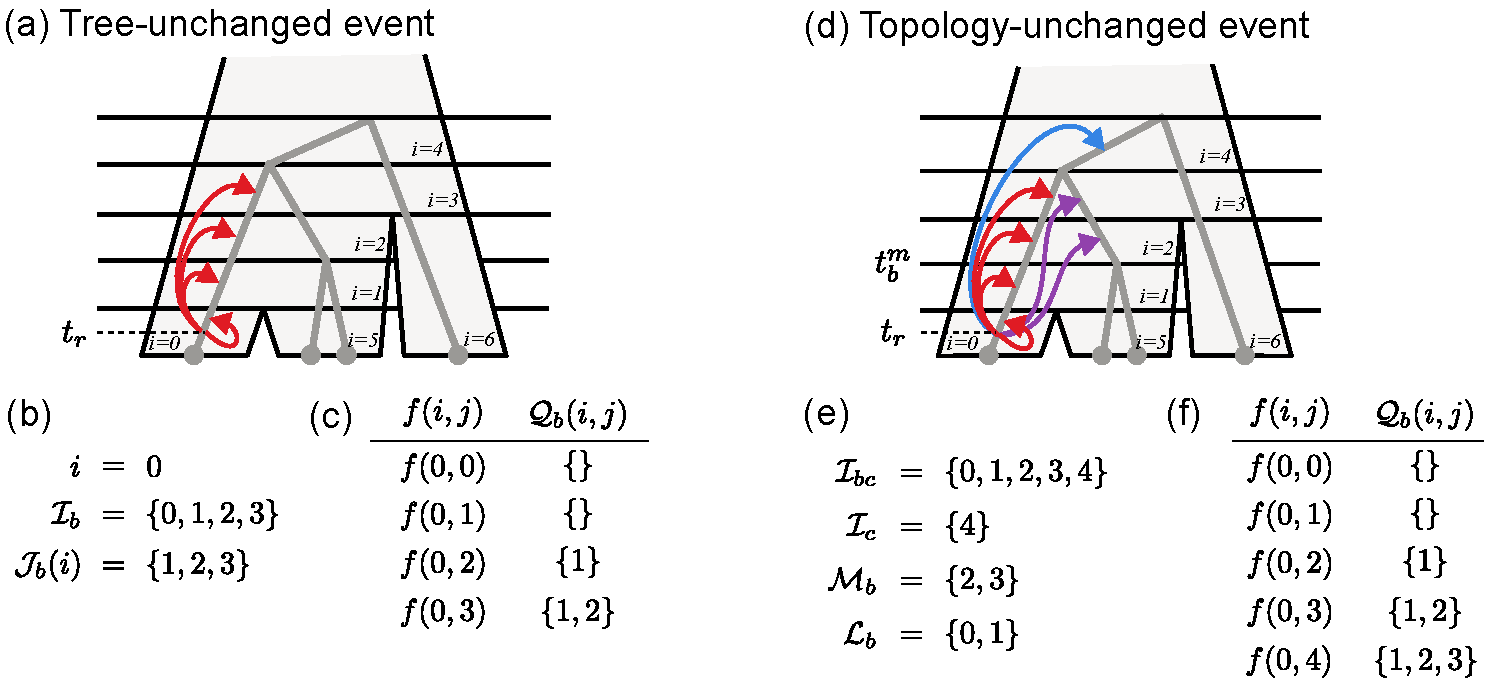
\includegraphics[width=0.99\textwidth]{figures/current/Fig3-interval-functions.pdf}
	\caption{
		% Rates of coalescence are piece-wise constant within discrete intervals 
		% of the genealogy embedding table. 
		\textcolor{red}{The probability of each categorical
		recombination event type is calculated from the probability
		of recombination occurring on a specific gene tree branch and of
		the resulting detached subtree re-coalescing with an available
		branch above that event.}
		\textcolor{red}{\sout{
		The probabilities of different recombination event types are calculated using piece-wise constant probabilities of recombination within discrete
		intervals.}}
		% probability statements for recombination occurring
		% at time $t_r$ in interval $i$ and re-coalescing in interval $j$. 
		(a) The probability of a ``no-change" (tree-unchanged) event involves
		re-coalescing with the same branch on which recombination occurred,
		for which intervals are indexed using the variable $\mathcal{I}_b$.
		%, or $\mathcal{J}_b(i)$. 
		(b) Indexing variables for calculating 
		\textcolor{red}{\sout{tree}}
		\textcolor{red}{no}-change probabilities. The indexing variable $\mathcal{I}_b$ records all
		intervals on branch $b$\textcolor{red}{; \sout{, and}}
		the recombination event for this example occurs in interval $i$=0.
		$\mathcal{J}_b(i)$ returns all intervals
		in $\mathcal{I}_b$ above interval $i$.
		(c,f) The function $f(i,j)$ returns the probability that a subtree that detached 
		in interval $i$ will re-coalesce in interval $j$. This involves excluding
		the probability of re-coalescence in intervals between $i$ and $j$, which are 
		indexed as $\mathcal{Q}_b(i,j)$. 
		(d) The probability of a topology-unchanged event involves re-coalescing with the 
		same branch on which recombination occurred, or with its parent or sibling branches. 
		%(e) Additional indexing variables return intervals on the parent branch 
		%($\mathcal{I}_c$), or the sibling branch above ($\mathcal{M}_b$) or below 
		%($\mathcal{L}_b$) the time at which it overlaps in the same species tree interval
		%as branch $b$, termed $t_b^m$.
		(e) Additional indexing variables return intervals on the parent branch 
		($\mathcal{I}_c$), or branch $b$ above ($\mathcal{M}_b$) or below 
		($\mathcal{L}_b$) the time ($t_b^m$) at which it overlaps in the same species tree interval 
		as its sibling branch.
	}
	\label{fig:fig3}
\end{figure}


% PREVIOUS APPROVED EQUATION 3
\begin{equation}
\begin{aligned}
	&\mathbb{P}(\text{no-change} | \mathcal{S},\mathcal{G},b,t_r) = 
	\frac{1}{k_i} + 
	f(i,i) \exp \bigg\{ \frac{k_i}{2n_i} t_r \bigg\} +
	\sum_{j \in \mathcal{J}_b(i)} f(i,j) \exp \bigg\{ \frac{k_i}{2n_i} t_r\bigg\}
	% \sum_{j=i+1}^{\mathcal{I}_b - 1} f(i,j) \exp\bigg\{\frac{a_i}{2n_i}t_r\bigg\} 
\end{aligned}
\end{equation}


\noindent This equation is simplified by use of the function $f(i,j)$
to return the piece-wise constant probabilities of re-coalescence between
pairs of intervals. When $j$=$i$, this expression involves the probability of 
coalescing over the remaining length of interval $i$ above $t_r$; 
when $j$>$i$ it involves the probability of coalescing in interval 
$j$ and not coalescing in interval $i$ or any other intervals 
between $i$ and $j$. For this latter process, we define another
indexing variable, $\mathcal{Q}_b(i,j)$ = $\{q \in \mathcal{I}_b ~|~ j > q > i\}$, 
for iterating over the ordered intervals above $i$ and below $j$ 
on branch $b$ (e.g., Fig.~\ref{fig:fig3}c).
The function $f(i,j)$ forms the core of the MS-SMC algorithm and 
will reappear in several later equations. 
\textcolor{red}{For didactic purposes, a step-by-step demonstration 
of equation (3) is shown in Fig.~\ref{fig:figS-tree-equations} of the Appendix.}

\begin{equation}
\begin{aligned}	
	f(i,j) = 
	\begin{dcases}
		- \frac{1}{k_i} \exp \bigg\{-\frac{k_i}{2n_i}\mu_i \bigg\}, 
		& \text{if } i=j\\
		% 
		\frac{1}{k_j} \left(1 - \exp \bigg\{ -\frac{k_j}{2n_j} d_j \bigg\} 
		\right)
		\exp \bigg\{ -\frac{k_i}{2n_i}\mu_i - 
		\sum_{q \in \mathcal{Q}_b(i,j)} \frac{k_q}{2n_q} d_q \bigg \}, 
		& \text{if } i<j\\
		% 
		0, 
		& \text{if } i>j\\
	\end{dcases}
\end{aligned}
\end{equation}

% PREVIOUS APPROVED EQUATION 4
% \begin{equation}
% \begin{aligned}
% 	% &P_{ii} = - \frac{1}{a_i} \exp \bigg\{-\frac{a_i}{n_i}(t_i^u - t_r) \bigg\} 
% 	&P_{ii} = - \frac{1}{a_i} \exp \bigg\{-\frac{a_i}{n_i}\sigma_{i + 1} \bigg\} 	
% \end{aligned}
% \end{equation}

% \begin{equation}
% \begin{aligned}
% 	&P_{ij} = 
% 	\left( \frac{1}{a_j} (1 - \exp \bigg\{ -\frac{a_j}{n_j} d_j \bigg\} \right)
% 	\times
% 	\exp \bigg\{ -\frac{a_i}{n_i}\sigma_{i+1} - 
% 	\sum_{q=i+1}^{j-1} \frac{a_q}{n_q} d_q \bigg \}
% \end{aligned}
% \end{equation}


% \begin{equation}
% \begin{aligned}
% 	&\mathbb{P}(\textrm{tree unchanged} | b,t,\mathcal{T},\mathcal{S}) = \frac{1}{a_i} +P_{ii}e^{\frac{a_i}{n_i}t}+ \sum_{k=i+1}^{\mathcal{I}_b-1} e^{\frac{a_i}{n_i}t} P_{ik}, \\
% 	&\text{where} \\
% 	&P_{ii} = - \frac{1}{a_i}e^{-\frac{a_i}{n_i}\sigma_{i+1}}, \\
% 	&\text{and} \\
% 	&P_{ik} = \exp\left(-\frac{a_i}{n_i}\sigma_{i+1}-\sum_{q=i+1}^{k-1} \frac{a_q}{n_q}T_q\right)\left(\frac{1}{a_{k}}(1-e^{-\frac{a_{k}}{n_{k}}T_{k}})\right),
% \end{aligned}
% \end{equation}

% \subsubsection{Probability that recombination on branch $b$ will not change the tree:}
\noindent By integrating equation 3 across all times at which recombination could
have occurred on branch $b$ (assuming a uniform recombination rate through time) 
we obtain the probability that recombination anywhere on this branch does not 
change the tree:

% \begin{equation*}
% 	\mathbb{P}(\textrm{no-change} | \mathcal{S},\mathcal{G},b) = 
% 	\frac{1}{t^u_b-t^l_b} \int_{t_b^l}^{t_b^u} 
% 	\mathbb{P}(\textrm{no-change} | \mathcal{S},\mathcal{G},b,t)dt
% \end{equation*}

\begin{equation}
\begin{aligned}
	% &
	\mathbb{P}(\textrm{no-change} | \mathcal{S},\mathcal{G},b) = 
	% \frac{1}{t^u_b-t^l_b} \int_{t_b^l}^{t_b^u} 
	% \mathbb{P}(\textrm{no-change} | \mathcal{S},\mathcal{G},b,t)dt =
	% \\
	% & 
	\frac{1}{t_b^u - t_b^l}
	\sum_{i \in \mathcal{I}_b} \left[\frac{1}{k_i} d_i + 
	% \Bigg(
	\frac{2n_i}{k_i} 
	\sum_{j \in \mathcal{I}_b}f(i,j)
	\bigg(
		\exp\bigg\{\frac{k_i}{2n_i}\mu_i \bigg\} - 
		\exp\bigg\{\frac{k_i}{2n_i}\sigma_i \bigg\}
	\bigg)\right]
	% \Bigg)
\end{aligned}
\end{equation}
% \begin{equation}
% 	= \frac{1}{t^u_b - t^l_b}
% 	\sum_{i=0}^{\mathcal{I}_b-1} \frac{1}{a_i} d_i + 
% 	\frac{2n_i}{a_i} 
% 	\bigg(
% 		\exp\bigg\{\frac{a_i}{2n_i}\sigma_{i+1}\bigg\} - 
% 		\exp\bigg\{\frac{a_i}{2n_i}\sigma_i\bigg\}
% 	\bigg)
% 	\bigg(\sum_{j=i}^{\mathcal{I}_b-1}f(i,j)\bigg)
% \end{equation}


% \subsubsection{Probability that a recombination event will not change the tree:}
\noindent Finally, by summing across all branches on the tree 
while weighting each one by its relative proportion of edge length,
% while assuming a uniform recombination rate through time and across branches, 
we get the probability that a recombination event occurring anywhere on 
$\mathcal{G}$ will result in a no-change event. %category 1 outcome.

\begin{equation}
	\mathbb{P}(\text{no-change} | \mathcal{S},\mathcal{G}) = 
	\sum_{b \in \mathcal{G}}
	\left[\frac{t^u_b - t^l_b}{L(\mathcal{G})}\right]
	\mathbb{P}(\text{no-change} | \mathcal{S},\mathcal{G},b)
\end{equation}


\subsubsection{Waiting distances to no-change and tree-change events}
Under the SMC', recombination is modeled as a Poisson point process 
such that the time between recombination events is exponentially distributed 
with rate parameter $\lambda_r$: the product of the per-site
per-generation recombination rate and summed branch lengths of
the current genealogy \citep{wiuf_ancestry_1999} (equation 7).
The likelihood of an observed distance ($x$) between recombination
events spatially along the genome, in units of base pairs, can thus 
be calculated from the exponential probability density function 
(equation 8).
% is distributed as an exponential probability density.

% This can be treated as a 
% Poisson point process, with rate parameter $\lambda_r$ (equation 7), 
% to model the waiting distances ($x$) between recombination events 
% as to an exponential probability distribution (equation 8).

\begin{equation}
	\lambda_{r} = L(\mathcal{G}) \times r
\end{equation}


\begin{equation}
	f(x; \lambda_r) = \lambda_r e^{-\lambda_r x}
\end{equation}

%\noindent Because a no-change type event is a subset of all possible types of
%recombination events, and we have derived its probability, we can now calculate 
\noindent Having derived the probability that an individual recombination event 
is of the no-change type, we can now calculate 
the rate of no-change type events as a proportion of the rate of all types of 
recombination events. 
Here, waiting distances continue to be exponentially distributed. 
However, the new rate parameter $\lambda_n$ is reduced proportionally by 
the probability that recombination causes no change to the genealogy
(equation 9). Similarly, because a tree-change event is the opposite 
of a no-change event, its probability is one minus the probability
of no-change (equation 10). This yields rate parameter $\lambda_g$ for 
the exponential probability distribution of waiting distances between 
tree-change events.

\begin{equation}
	\lambda_{n} = 
	L(\mathcal{G}) \times r \times 
	\mathbb{P}(\text{no-change} | \mathcal{S},\mathcal{G})
\end{equation}

% We can thus modify this equation to instead yield a probability
% density for waiting distances to a recombination event that causes a 
% tree change. 

\begin{equation}
	\lambda_{g} = 
	L(\mathcal{G}) \times r \times 
	(1 - \mathbb{P}(\text{no-change} | \mathcal{S},\mathcal{G}))
\end{equation}

% \begin{equation}
% \begin{aligned}
% 	&p_r(d|\mathcal{T},\mathcal{S}) = r\alpha_\mathcal{S}(\mathcal{T})L(\mathcal{T})\exp\left[-r\alpha_\mathcal{S}(\mathcal{T})L(\mathcal{T})d\right]\textrm{,} \\
% 	&where \\
% 	&\alpha_\mathcal{S}(\mathcal{T})=1-\mathbb{P}(\textrm{tree unchanged} | \mathcal{T},\mathcal{S})
% \end{aligned}
% \end{equation}


\subsubsection{Probability of topology-change}
% Deriving probabilities of changes in the genealogical topology}

We next derive an analogous probability distribution for waiting distances 
between topology-change events.
% This involves events 
% representing a subset of possible tree-change events. 
Similar to our approach for calculating tree-change probabilities as the opposite of those for a 
no-change (tree-unchanged) event, here we calculate topology-change probabilities as the 
opposite of those for a topology-unchanged event. Topology-unchanged events represent the union of 
all no-change events and the subset of possible tree-change events 
that only affect branch lengths but not the topology. 
Our approach for calculating these probabilities follows closely to that of \citet{deng_distribution_2021}.
% in which 
% where the topology
% This involves excluding 
% events that affect only coalescence times but not the topology. We refer
% to this set of events as "topology-unchanged".
% of categories 2 and 3 to isolate the waiting distance to a category 4 event. 
In order to isolate re-coalescence events that do not change the topology,
% only affect branch
% lengths from those that affect the topology 
we must take into account which specific branches the detached subtree from 
branch $b$ re-coalesces with. The relevant branches are its source ($b$), 
its sibling ($b'$), and its parent ($c$) (Fig.~\ref{fig:fig3}d). 
If the subtree re-coalesces with $b$, no change occurs; if it re-coalesces
with $b'$, the topology remains the same but a coalescent time is shortened;
and if it re-coalesces with $c$, the topology remains the same but a coalescent 
time is lengthened. A re-coalescence with any other branch will change the topology.
% Once again, we start by deriving branch-specific probabilities and then sum 
% these across all branches on a genealogy. 


% It $b$ re-coalesces
% with any other branch it would cause a topology change instead of a tree
% change, which we address after this section.

% The primary difference in this approach is that for any 
% branch $b$ we have to also consider coalescence possibilities with the branch above it 
% (branch $c$) and the branch with which it coalesces (branch $b'$). 



% If $b$ and $b'$ are in the same species tree itnervall...
% such that by indexing from $m$ to $\mathcal{I}_b$ we can visit all 
% intervals that are shared by the sibling branches. 

% We also introduce a new variable, $t_b^m$, which corresponds to the lowest point
% at which branch $b$ can potentially coalesce with its sibling, branch $b'$. 
% $t_b^m$ will always be the maximum of three values: the time at which $b$ and 
% $b'$ are separated by a species divergence (if at all), the lowest point on 
% branch $b'$ (i.e., $t_{b'}^l$), and $t_b^l$. Interval
% $m$, which is simply the interval whose lower bound is $t_b^m$, is used to break 
% the equations into multiple parts and therefore is present as a start and 
% stop point for some summations in this section.


% \subsubsection{Probability recombination at $t_r$ on branch $b$ does not change the topology:}
% Unlike the previous approach, where we 
% calculated the probability of a no-change event, we now calculate this probability 
% in addition to the probability of a change that affects only coalescent times and not the topology. 
To index over relevant intervals across the three branches on which re-coalescence
can occur, we define several additional variables. The lowest time point in which both 
$b$ and $b'$ are present and exist within the same species tree interval is labeled 
$t_b^m$. For a branch $b$ with intervals $\mathcal{I}_b$, the subset of intervals 
below $t_b^m$ is $\mathcal{L}_b$, and the subset above is $\mathcal{M}_b$. 
The union of the sets of intervals on branches $b$ and $c$ is $\mathcal{I}_{bc}$
(Fig.~\ref{fig:fig3}e).
% \hl{however, we additionally incorporate changing coalescent rates 
% through different species tree intervals, as well as account for the 
% constraint that sister lineages may not initially exist in 
% the same species tree interval.}
% To do this, 

Once again, we begin by assuming knowledge of the branch on which a 
recombination event occurs and of that event's timing. This problem can be broken 
into two distinct cases: when $t_r$ occurs below $t_b^m$, and when it 
occurs above $t_b^m$. The former requires integrating over additional 
intervals on $b$ that are not shared with $b'$. Over all intervals
on the three relevant branches, these equations use the function 
$f(i,j)$ to return the piecewise constant probabilities where recombination 
occurs in interval $i$ and re-coalesces in interval $j$ (Fig.~\ref{fig:fig3}f).
% As before, this involves iterating over intervening intervals
% between $i$ and $j$ if present (Fig.~\ref{fig:fig3}f).
\textcolor{red}{We provide a didactic example of the Equation 11
calculation in Fig.~\ref{fig:figS-topo-equations} of the Appendix.}


% a category 1 event, we %are now trying to 
% now 
% calculate the probability of an event falling into categories 1, 2, or 3. 
% To do this, we must immediately break the problem into two different cases: 
% one in which $t_r$ occurs lower than $t_b^m$, and one in which $t_r$ is higher than $t_b^m$.
% when $t_r$ occurs below $t_b^m$, and when it occurs above $t_b^m$.
% \paragraph{First case --} Given $t_r$ $<$ $t_b^m$ and 
% $t_r \in [\sigma_i, \sigma_{i+1}] \subset [t_b^l,t_b^m]$



% the subsequent two intervals after $t_b^m$, the detached lineage can re-coalesce
% % either with it 
% In this case, we have integrated coalescence probabilities through three sections 
% in which a re-coalescence can produce a category 1, 2, or 3 event: the lower part 
% of branch $b$ when the disconnected branch can reconnect with itself, the upper 
% part of branch $b$ when it can reconnect with either itself or with its sibling,
% and all of branch $c$, with which a coalescent would lengthen branches without 
% changing the topology (Fig.~\ref{fig:fig3}a).

% \begin{equation}
% 	\mathbb{P}(\textrm{topology unchanged} | \mathcal{S},\mathcal{G},b,t_r) = 
% 	\frac{1}{a_i} + \sum_{j=i}^{\mathcal{I}_{b+c}-1}P_{ik}\exp\left\{\frac{a_i}{n_i}t_r\right\} + 
% 	\sum_{j=m}^{\mathcal{I}_b-1}P_{ik}\exp\left\{\frac{a_i}{n_i}t_r\right\}
% \end{equation}

% \begin{equation}
% 	\mathbb{P}(\textrm{topology unchanged} | \mathcal{S},\mathcal{G},b,t_r) = 
% 	\frac{1}{a_i} + \sum_{j=i}^{\mathcal{I}_{bc}-1} 
% 	f(i,j) \exp\left\{\frac{a_i}{n_i}t_r\right\} + 
% 	\sum_{j=m}^{\mathcal{I}_b-1}f(i,j)\exp\left\{\frac{a_i}{n_i}t_r\right\}
% \end{equation}

% \small
% \begingroup\makeatletter\def\f@size{9}\check@mathfonts
\begin{equation}
\begin{aligned}
	&\mathbb{P}(\textrm{topology-unchanged} | \mathcal{S},\mathcal{G},b,t_r)=
	\\
	&\begin{dcases}
		\frac{1}{k_i} + 
		\sum_{j \in \mathcal{I}_{bc}} f(i,j) \exp \bigg\{ \frac{k_i}{2n_i}t_r \bigg\} + 
		\sum_{j \in \mathcal{M}_b} f(i,j) \exp \bigg\{ \frac{k_i}{2n_i}t_r \bigg\}, 
		& \text{if } t_r < t_b^m \\
		\\
		2\bigg(
			\frac{1}{k_i} + 
			\sum_{j \in \mathcal{I}_b} f(i,j) \exp \bigg\{ \frac{k_i}{2n_i}t_r \bigg\}
		\bigg) + 
		\sum_{j \in \mathcal{I}_c} f(i,j) \exp\bigg\{ \frac{k_i}{2n_i}t_r \bigg\},
		& \text{if } t_r \ge t_b^m \\
	\end{dcases}
\end{aligned}
\end{equation}

% \begin{equation}
% 	\mathbb{P}(\textrm{topology-unchanged} | \mathcal{S},\mathcal{G},b,t_r)=
% 	\begin{dcases}
% 		\frac{1}{a_i} + 
% 		\sum_{j=i}^{\mathcal{I}_{bc}-1} f(i,j) \exp\left\{\frac{a_i}{2n_i}t_r\right\} + 
% 		\sum_{j=m}^{\mathcal{I}_b-1} f(i,j) \exp\left\{\frac{a_i}{2n_i}t_r\right\}, 
% 		& \text{if } t_r < t_b^m \\
% 		\\
% 		2\bigg(
% 			\frac{1}{a_i} + 
% 			\sum_{j=i}^{\mathcal{I}_{b}-1} f(i,j)\exp\bigg\{\frac{a_i}{2n_i}t_r\bigg\}
% 		\bigg) + 
% 		\sum_{\mathcal{I}_b}^{\mathcal{I}_{bc}-1} f(i,j) \exp\bigg\{
% 			\frac{a_i}{2n_i}t_r
% 		\bigg\},
% 		& \text{if } t_r \ge t_b^m \\
% 	\end{dcases}
% \end{equation}

% \normalsize
% \endgroup


% \paragraph{Second case --} Given $t_r$ $>$ $t_b^m$ and 
% $t_r \in [\sigma_i, \sigma_{i+1}] \subset [t_b^m,t_b^u]$ is is necessary

% \noindent In the second case (Fig.~\ref{fig:fig3}b), where $t_r$ $>$ $t_b^m$ and 
% $t_r \in [\sigma_i, \sigma_{i+1}] \subset [t_b^m,t_b^u]$ 
% it is only necessary to integrate over probabilities across a subset of the 
% second section, and across the entire third section described above, from 
% which the following equation can be derived:
% % In this second case $t_r$ occurs after $t_b^m$, such that there are only 
% two distinct sections over which to integrate probabilities of tree changes, 
% corresponding to sections 2 and 3 from the case above (Fig.~\ref{fig:fig3}b).
% In the first section $b$ can re-coalescen with either $b$ or $b'$, 
% is when the detached branch can re-coalesce with itself or its sibling, 
% and the second when it can coalesce with its parent 

% \begin{equation}
% 	\mathbb{P}(\textrm{topology unchanged} | \mathcal{S},\mathcal{G},b,t_r) = 
% 	2\left(\frac{1}{a_i} + \sum_{k=i}^{\mathcal{I}_{b}-1}P_{ik}\exp\left\{\frac{a_i}{n_i}t_r\right\}\right) + 
% 	\sum_{\mathcal{I}_b}^{\mathcal{I}_{b+c}-1}P_{ik}\exp\left\{\frac{a_i}{n_i}t_r\right\}
% \end{equation}

% \begin{equation}
% 	\mathbb{P}(\textrm{topology unchanged} | \mathcal{S},\mathcal{G},b,t_r) = 
% 		2\bigg(
% 			\frac{1}{a_i} + \sum_{j=i}^{\mathcal{I}_{b}-1}f(i,j)\exp\bigg\{
% 				\frac{a_i}{n_i}t_r
% 			\bigg\}
% 		\bigg) + 
% 		\sum_{j=\mathcal{I}_b}^{\mathcal{I}_{bc}-1}f(i,j)\exp\bigg\{
% 			\frac{a_i}{n_i}t_r
% 		\bigg\}
% \end{equation}

% \subsubsection{Probability that a recombination event on branch $b$ will not change the topology:}
\noindent Next, the probability of a topology-unchanged event given recombination 
anywhere on a branch can be derived by integrating the previous equation 
over the entire length of a branch.
% We next present the probability that a recombination event occurring on a focal 
% branch $b$ will not change the tree topology -- i.e., it will result in one of the 
% other two outcomes for which we have derived probabilities: no change or tree change.
% As in Section 2.4, 
 % across the entire length of a branch. 
Here, the terms $p_{b,1}$ and $p_{b,2}$ correspond to recombination occurring
on branch $b$ during a time that falls into either of the two cases in equation 11.%, below or above $t_b^m$. 
% associated with the two cases described above and in Fig.~\ref{fig:fig3}a-b:
% , the lowest interval...the location of $t_b^m$.}
% through the solution that specifies both a specific branch and time. 

% \begin{equation}
% \begin{aligned}
%     &\mathbb{P}(\textrm{topology unchanged} | \mathcal{S},\mathcal{G},b) = 
%     \frac{1}{t_b^u-t_b^l}\left[\sum_{i=0}^{m-1}p_{b,1}^{(i)}+\sum_{i=m}^{\mathcal{I}_b-1}p_{b,2}^{(i)}\right] \\
%     &where: \\
%     &p_{b,1}^{(i)} = \frac{1}{a_i}\left[d_i+n_i\left(\exp\left\{\frac{a_i}{n_i}\sigma_{i+1}\right\}-\exp\left\{\frac{a_i}{n_i}\sigma_i\right\}\right)\left(\sum_{k=i}^{\mathcal{I}_{b+c}-1}P_{ik}+\sum_{k=m}^{\mathcal{I}_b-1}P_{ik}\right)\right] \\
%     &and: \\
%     &p_{b,2}^{(i)} = \frac{1}{a_i}\left[2d_i + n_i\left(\exp\left\{\frac{a_i}{n_i}\sigma_{i+1}\right\}-\exp\left\{\frac{a_i}{n_i}\sigma_{i}\right\}\right)\left(2\sum_{k=i}^{\mathcal{I}_b-1}P_{ik}+\sum_{k=\mathcal{I}_b}^{\mathcal{I}_{b+c}-1}P_{ik}\right)\right]
%     \end{aligned}
% \end{equation}

\begin{equation}
\begin{aligned}
	&\mathbb{P}(\textrm{topology-unchanged} | \mathcal{S},\mathcal{G},b) = 
	\frac{1}{t_b^u - t_b^l} \Bigg[
		\sum_{i \in \mathcal{L}_b} p_{b,1}^{(i)} + 
		\sum_{i \in \mathcal{M}_b} p_{b,2}^{(i)}
	\Bigg]
	\\
	&~~where: 
	\\
	&p_{b,1}^{(i)} = 
		\frac{1}{k_i} \Bigg[
			d_i + 2n_i \Bigg(
				\exp\bigg\{ \frac{k_i}{2n_i}\mu_i \bigg\} - 
				\exp\bigg\{ \frac{k_i}{2n_i}\sigma_i\bigg\}
			\Bigg)
		\Bigg(
			\sum_{j \in \mathcal{I}_{bc}}f(i,j) + \sum_{j \in \mathcal{M}_b}f(i,j)
		\Bigg)
	\Bigg]
	\\
	&~~and: 
	\\
	&p_{b,2}^{(i)} = 
		\frac{1}{k_i} \Bigg[
			2d_i + 2n_i \Bigg(
				\exp\bigg\{\frac{k_i}{2n_i}\mu_i \bigg\} - 
				\exp\bigg\{\frac{k_i}{2n_i}\sigma_{i} \bigg\}
			\Bigg)
		\Bigg(
			2\sum_{j \in \mathcal{I}_b} f(i,j) + \sum_{j \in \mathcal{I}_c} f(i,j)
		\Bigg)
	\Bigg]
    \end{aligned}
\end{equation}


% \begin{equation}
% \begin{aligned}
% 	&\mathbb{P}(\textrm{topology-unchanged} | \mathcal{S},\mathcal{G},b) = 
% 	\frac{1}{t_b^u - t_b^l} \Bigg[
% 		\sum_{i=0}^{m-1}p_{b,1}^{(i)} + 
% 		\sum_{i=m}^{\mathcal{I}_b-1}p_{b,2}^{(i)}
% 	\Bigg]
% 	\\
% 	&where: 
% 	\\
% 	&p_{b,1}^{(i)} = 
% 		\frac{1}{a_i} \Bigg[
% 			d_i + 2n_i \bigg(
% 				\exp\bigg\{\frac{a_i}{2n_i}\sigma_{i+1}\bigg\} - 
% 				\exp\bigg\{\frac{a_i}{2n_i}\sigma_i\bigg\}
% 			\bigg)
% 		\bigg(
% 			\sum_{j=i}^{\mathcal{I}_{bc}-1}f(i,j) + \sum_{j=m}^{\mathcal{I}_b-1}f(i,j)
% 		\bigg)
% 	\Bigg]
% 	\\
% 	&and: 
% 	\\
% 	&p_{b,2}^{(i)} = 
% 		\frac{1}{a_i} \Bigg[
% 			2d_i + 2n_i \bigg(
% 				\exp\bigg\{\frac{a_i}{2n_i}\sigma_{i+1}\bigg\} - 
% 				\exp\bigg\{\frac{a_i}{2n_i}\sigma_{i}\bigg\}
% 			\bigg)
% 		\bigg(
% 			2\sum_{j=i}^{\mathcal{I}_b-1}f(i,j) + \sum_{j=\mathcal{I}_b}^{\mathcal{I}_{bc}-1}f(i,j)
% 		\bigg)
% 	\Bigg]
%     \end{aligned}
% \end{equation}


% \subsubsection{Probability that a recombination event will not change the topology:}
\noindent Finally, by summing equation 12 across all branches on a 
genealogy while weighting each by its proportion of summed branch lengths,
we get the probability that a recombination event falling 
uniformly on the genealogy will result in a topology-unchanged event.

\begin{equation}
\begin{aligned}
	&\mathbb{P}(\textrm{topology-unchanged} | \mathcal{S},\mathcal{G})
	% \\
	= \sum_{b \in \mathcal{G}}\frac{t_b^u - t_b^l}{L(\mathcal{G})} 
	\times 
	\mathbb{P}(\textrm{topology-unchanged} | \mathcal{S},\mathcal{G},b)
	\\
	&
	= \frac{1}{L(\mathcal{G})} \sum_{b \in \mathcal{G}}
	\bigg[ 
		\sum_{i \in \mathcal{L}_b} p_{b,1}^{(i)} +
		\sum_{i \in \mathcal{M}_b} p_{b,2}^{(i)}
	\bigg]
\end{aligned}
\end{equation}

\subsubsection{Waiting distance to topology-change events}
A recombination event either does or does not change the topology
of a genealogy, and we can therefore get the probability of a 
topology-change event using our topology-unchanged probability statement.
As with the previous waiting distance distributions, the distance between
topology-change events given a parameterized MSC model can be 
modeled as an exponential probability distribution. 
Similar to how a rate parameter was derived for the distribution 
of waiting distances until a recombination event (equation 7), 
no-change event (equation 9), or tree-change event (equation 10), 
a rate parameter $\lambda_t$ can be calculated from equation 13 for 
the probability of a topology-change event. 
% from equation 13 
% to get the probability of a topology-change event (equation 14). 
 % density for the waiting distance until 
% a topology-change event: %, given a genealogy and an MSC model:

\begin{equation}
	\lambda_{t} = 
	L(\mathcal{G}) \times r \times 
	(1 - \mathbb{P}(\text{topology-unchanged} | \mathcal{S},\mathcal{G}))
\end{equation}


Unlike the exact solution for the expected waiting distance to a  
tree-change, the waiting distance for a topology-change is an
approximation. This is because topology-change probabilities are not 
guaranteed to be homogeneous across some distance of the genome between 
topology-change events, since intermediate tree-change events could occur
(e.g., the second and third recombination events in Fig.~\ref{fig:ARG-cartoon}).
We examine this and other potential sources of bias in our validations
below and in the Supplementary Materials.

% This is because the product of $L(\mathcal{G})$ and 
% the probability of a topology-changing recombination event
% does not change significantly 
% (longer genealogies are more likely to experience topology-change).

% Below, we demonstrate the accuracy of our approach, and investigate 
% the potential for biases caused by approximation, by validating our
% results relative to coalescent simulations with recombination.

% For example, when branch lengths become very long the expected 
% waiting distance to the next recombination event becomes very small, 
% and similarly the probability of topology-change decreases. 
% Conversely, if branch lengths are as short as possible within the 
% constraints of a species tree model, waiting distances between 
% events will be longer, and more likely to change the topology, since any 
% new sampled ancestor is more likely to be deeply coalesced. 
% Thus, while lengthening of branch length decreases the probability of 
% topology-change it increases the frequency of overall recombination events, 
% and vice versa, such that tree-change events have little overall effect 
% on the probability of topology-change. 
% Later, we validate 

% by showing that our equations yield accurate 
% waiting distances when compared to coalescent simulations
% even when the ratio of tree to topology changes is high.
% This expectation is investigated below using coalescent simulations.

% , for example, consider the extreme
% case )
% Even as branch lengths increase, reducing the waiting time to the 
% next recombination event, the probability that %the recombination event 
% this event will change the topology decreases. 
% Therefore, we follow their approach by approximating the waiting distance to
% a change in topology using an exponential probability density 
% distribution 
% with the following rate:

%\begin{equation}
%\begin{aligned}
%	&p_r(d|\mathcal{G},\mathcal{S}) = r\beta_\mathcal{S}(\mathcal{G})L(\mathcal{G})\exp\left[-r\beta_\mathcal{S}(\mathcal{G})L(\mathcal{G})d\right]\textrm{,} \\
%	&where \\
%	&\beta_\mathcal{S}(\mathcal{G})=1-\mathbb{P}(\textrm{topology unchanged} | \mathcal{G},\mathcal{S}).
%\end{aligned}
%\end{equation}


%%%%%%%%%%%%%%%%%%%%%%%%%%%%%%%%%%%%%%%%%%%%%%%%%%%%%%%%%%%%%%%%%%%%%%%%%%%
%%%%%%%%%%%%%%%%%%%%%%%%%%%%%%%%%%%%%%%%%%%%%%%%%%%%%%%%%%%%%%%%%%%%%%%%%%%
%%%%%%%%%%%%%%%%%%%%%%%%%%%%%%%%%%%%%%%%%%%%%%%%%%%%%%%%%%%%%%%%%%%%%%%%%%%
%%%%%%%%%%%%%%%%%%%%%%%%%%%%%%%%%%%%%%%%%%%%%%%%%%%%%%%%%%%%%%%%%%%%%%%%%%%
%%%%%%%%%%%%%%%%%%%%%%%%%%%%%%%%%%%%%%%%%%%%%%%%%%%%%%%%%%%%%%%%%%%%%%%%%%%
%%%%%%%%%%%%%%%%%%%%%%%%%%%%%%%%%%%%%%%%%%%%%%%%%%%%%%%%%%%%%%%%%%%%%%%%%%%
%%%%%%%%%%%%%%%%%%%%%%%%%%%%%%%%%%%%%%%%%%%%%%%%%%%%%%%%%%%%%%%%%%%%%%%%%%%
%%%%%%%%%%%%%%%%%%%%%%%%%%%%%%%%%%%%%%%%%%%%%%%%%%%%%%%%%%%%%%%%%%%%%%%%%%%
%%%%%%%%%%%%%%%%%%%%%%%%%%%%%%%%%%%%%%%%%%%%%%%%%%%%%%%%%%%%%%%%%%%%%%%%%%%
%%%%%%%%%%%%%%%%%%%%%%%%%%%%%%%%%%%%%%%%%%%%%%%%%%%%%%%%%%%%%%%%%%%%%%%%%%%
%%%%%%%%%%%%%%%%%%%%%%%%%%%%%%%%%%%%%%%%%%%%%%%%%%%%%%%%%%%%%%%%%%%%%%%%%%%
%%%%%%%%%%%%%%%%%%%%%%%%%%%%%%%%%%%%%%%%%%%%%%%%%%%%%%%%%%%%%%%%%%%%%%%%%%%
%%%%%%%%%%%%%%%%%%%%%%%%%%%%%%%%%%%%%%%%%%%%%%%%%%%%%%%%%%%%%%%%%%%%%%%%%%%
%%%%%%%%%%%%%%%%%%%%%%%%%%%%%%%%%%%%%%%%%%%%%%%%%%%%%%%%%%%%%%%%%%%%%%%%%%%
%%%%%%%%%%%%%%%%%%%%%%%%%%%%%%%%%%%%%%%%%%%%%%%%%%%%%%%%%%%%%%%%%%%%%%%%%%%
%%%%%%%%%%%%%%%%%%%%%%%%%%%%%%%%%%%%%%%%%%%%%%%%%%%%%%%%%%%%%%%%%%%%%%%%%%%
%%%%%%%%%%%%%%%%%%%%%%%%%%%%%%%%%%%%%%%%%%%%%%%%%%%%%%%%%%%%%%%%%%%%%%%%%%%
%%%%%%%%%%%%%%%%%%%%%%%%%%%%%%%%%%%%%%%%%%%%%%%%%%%%%%%%%%%%%%%%%%%%%%%%%%%
%%%%%%%%%%%%%%%%%%%%%%%%%%%%%%%%%%%%%%%%%%%%%%%%%%%%%%%%%%%%%%%%%%%%%%%%%%%
%%%%%%%%%%%%%%%%%%%%%%%%%%%%%%%%%%%%%%%%%%%%%%%%%%%%%%%%%%%%%%%%%%%%%%%%%%%


\section{Results}
% \label{sec:others}

\subsection{Implementation}
We have implemented our solutions for waiting distance calculations
under the MS-SMC in the Python package \emph{ipcoal} \citep{mckenzie_ipcoal_2020}.
This software includes functions that accept a parameterized MSC model and 
initial genealogy as input and return the probabilities of different 
recombination event types. These probabilities can be calculated for specific 
branches and times, for entire branches, or for entire genealogies. 
Functions are also available to calculate the expected waiting distances 
for a genealogy embedded in an MSC model,
and the likelihood 
\textcolor{red}{
of MSC model parameters given a distribution of waiting distances 
between tree-change or topology-change events in an ARG.
}
% of observed waiting distances in an ARG 
% an exponential probability density parameterized by the MS-SMC.
%Tree-based operations are performed with 
Our implementation is built upon \emph{toytree} \citep{eaton_toytree_2020}, 
\emph{scipy} \citep{2020SciPy-NMeth}, and 
\emph{numpy} \citep{harris2020array}, and 
uses jit-compilation with \emph{numba} 
\citep{lam2015numba}.
Below we use \emph{ipcoal} 
\textcolor{red}{v.0.5.0} 
to demonstrate the impact of 
MSC model parameters on waiting distances and to validate our solutions against 
expectations from coalescent simulations implemented in 
\emph{msprime} (v.1.1.1) \citep{baumdicker_efficient_2022}.
%and we investigate potential biases.
% models, visualizing results, and validating our equations.
Source code is available at \url{https://github.com/eaton-lab/ipcoal}.
Jupyter notebooks demonstrating the MS-SMC calculations and with 
reproducible code used for validations in this study are available
at \url{https://github.com/eaton-lab/waiting-distances}.



\begin{figure}
	\centering
	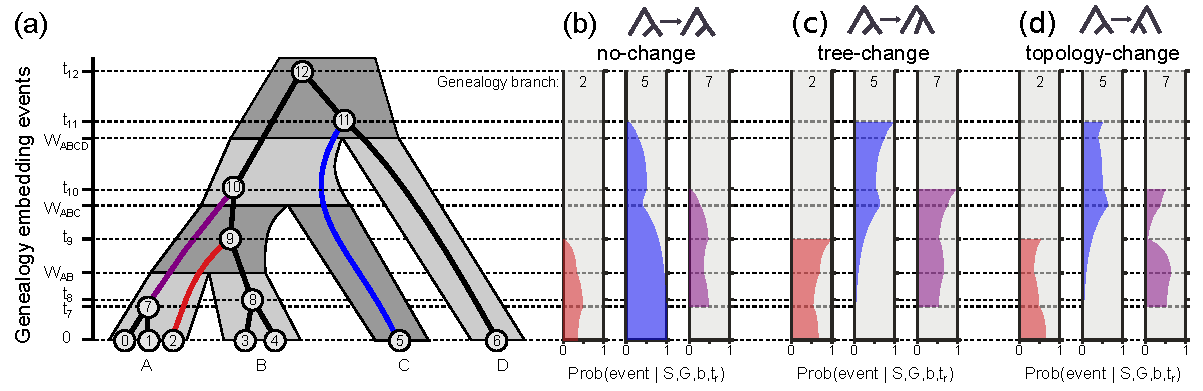
\includegraphics[width=0.99\textwidth]{figures/current/Fig4-embedding-with-probabilities.pdf}
	\caption{
		% \textcolor{red}{ \sout{
		% The MS-SMC models the probability of different recombination outcomes 
		% given a genealogy embedded in a multispecies coalescent (MSC) model.
		% (a) A parameterized MSC model is composed of multiple discrete population
		% intervals with associated effective population sizes ($N_e$) and divergence 
		% times ($W$). Given an embedded genealogy, each interval can be further divided 
		% at coalescence events (e.g., $t_9$) into a series of smaller intervals
		% with constant coalescent rates. The parameters of these intervals make up a 
		% genealogy embedding table (see Table 1).
		% The probabilities of each outcome as calculated under the MS-SMC 
		% are shown for three arbitrary branches. 
		% These probabilities are a function of the time ($t_r$) and branch 
		% on which recombination occurs.	
		% }}
		\textcolor{red}{
		The MS-SMC is a model of the probability of different categorical event
		outcomes given recombination occurring uniformly on a genealogy embedded
		in a parameterized MSC model (a). 
		% 
		A recombination event can cause one of three possible recombination 
		event types between two sequential genealogies in a genome: 
		\emph{no-change}, \emph{tree-change}, or \emph{topology-change}.
		% 
		The probability of these event types are calculated by integrating over
		each branch on the genealogy on which recombination can occur; which
		in turn is calculated by integrating over each position on a genealogy
		branch at which recombination can occur.
		% 
		(b-d) The probability that a recombination event causes a no-change, tree-change, or topology-change event, for the example genealogy 
		embedded in a species tree, was calculated for three selected 
		genealogy branches (2: red; 5: blue; and 7: purple), at each position
		along the branch where recombination could occur.
		}
		% , for each position along their length where recombination
		% cour
		% The probability of each event occuring 
		% the probabilities of recombination occurring on each branch and causing
		% the event type. 
		%  all
		% branches on which recombination could occur. The probability of each
		% event type on each branch is calculated by integrating over all positions
		% on that branch on which recombination could occur. 
		% probabilities are calculated by integrating over all 
		% positions along each genealogy branch where recombination could occur.
		% % 
		% (b-d) The probabilities of each event type are shown for each position
		% along the length of three selected genealogy 
		% probability of each event type calculated on each branch ($b$)
		% and over 
		% as a function of the
		% MSC model parameters ($\mathcal{S}$), genealogy ($\mathcal{G}$), and the
		% branch and timing on which recombination occurs ($b$, and $t_r$, 
		% respectively).
		% % 
		% % (a) Coalescence and species divergence events delimit intervals within
		% % species tree intervals within which the rate of coalescence is constant
		% % (dashed lines).
		% % (a) The event type probabilities are a 
		% % function of a genealogy embedded in a parameterized MSC model.
		% This is shown for 
		% % For the example genealogy and MSC model the probability of each event 
		% % type is shown for 
		% three selected genealogy branches (2: red; 5: blue; and 7: purple) computed
		% for each position along their branch lengths where recombination could occur.
		% }
	}
	\label{fig:edge-probabilities}
\end{figure}


% tree manipulationpaired with 
% Source code and example jupyter notebooks are available at
% \url{https://github.com/eaton-lab/ipcoal}, including validation against 
% coalescent simulations  software  paired with tree visualizations from
% % Our MS-SMC functions are implemented in the subpackage \emph{ipcoal.smc}. 
% Here we demonstrate
% the accuracy of our solutions relative to simulated tree sequences.
% Source code is available at 
% We adapted our solutions to python code, and we implemented them alongside the phylogenomic simulation package \emph{ipcoal} (an MSC-focused wrapper for the popular population genomic simulator \emph{msprime}) \citep{mckenzie_ipcoal_2020,baumdicker_efficient_2022}. Doing so facilitated three simple, illustrative analyses.

\subsection{Demonstration}
% First, when given a species tree and initial genealogy, we could examine the probability 
Given a parameterized MSC model and initial genealogy, the probabilities of 
different types of recombination outcomes can be calculated and visualized as 
a function of when and where recombination occurs. This is demonstrated on an 
imbalanced 4-tip species tree with constant effective population size 
% across branches %(see parameters in Table~S2), 
and with a genealogy of seven samples embedded, 
including three from lineage A, two from lineage B, and one from each of lineages
C and D (Fig.~\ref{fig:edge-probabilities}a). 
\textcolor{red}{(See Fig.~\ref{fig:figS-edge-probabilities} for details and
alternative parameterizations of this simulation.)}
% As a demonstration, t
The probabilities of no-change, tree-change, or topology-change events, 
given a recombination event occurring on a branch at a particular time 
(equations 3 and 11, respectively) are shown for three selected branches
on the example genealogy (Fig.~\ref{fig:edge-probabilities}b-d). 
Note that the probability of no-change and tree-change events 
are inversely related and sum to 1, since one or the other must occur at any 
%accompany any 
%occur as a consequence 
recombination event. By contrast, \textcolor{red}{the probability of} a 
topology-change event is a subset of the probability of a tree-change 
\textcolor{red}{event}; 
% recall that a topology-change event is 
it is a tree-change event where the detached branch re-coalesces with 
a branch other than itself, its sibling, or its parent.

% We then applied our solutions to calculate probabilities of changes given 
% ...Our species tree was proposed arbitrarily with a root height of 1e6 generations and 
% includes branch-specific effective population sizes (Table~S1). 
% Our sampling in the genealogy includes three individuals
% for population A, two individuals for population B, and one individual for each 
% population C and D. The exact parameterization for the model, as well as the 
% code to replicate the analysis, is documented in our supplementary notebooks.
% ...
 % tree model 
% of changes in the genealogy given a recombination event on a specific branch and at a 
% specific time. \textbf{Figure 3} illustrates the selection of three branches from a genealogy 
% embedded in a species tree model. The species tree 
% was unbalanced 
% is imbalanced
% with five tips, 
%had 
% and equal internode distances of 2.5e5 generations, 
% and had 
% with constant Ne of 2e5 across species tree intervals. 
% Parts 

In general, the probability of a no-change event decreases, and the probability
of a tree-change event increases, as recombination occurs closer to the top
\textcolor{red}{\sout{end}} of a \textcolor{red}{gene tree} branch (further back in time). 
This makes intuitive sense, since when 
recombination occurs at the top of a branch there is less time for it to re-coalesce 
with its same branch. Although this is a general trend, these probabilities do not 
behave monotonically \textcolor{red}{\sout{along the length of a branch} with respect
to time} as they would in a 
single-population model with constant $N_e$ \citep{deng_distribution_2021}.
Instead, probabilities increase or decrease through the length of each
interval as a function of the rates of coalescence in subsequent 
intervals and the probability that a detached lineage will 
re-coalesce in one of those intervals.

For example, consider \textcolor{red}{genealogy} branch 2, which exhibits an increase in the
probability of no-change through its first branch interval from time 0 to
$t_7$ but then a decrease through the next interval from $t_7$ to $W_{AB}$
(Fig.~\ref{fig:edge-probabilities}b).
The observed increase through the first interval is influenced by the fact that
a re-coalescence in the subsequent interval is more likely to cause a no-change
event, since that interval contains only two samples instead of three.
% up recombination occurs in this interval the more likely it is to re-coalesce
% in the next interval, where only two instead of three samples are present, such
% that a no-change event is more likely. 
%By contrast, within the second interval, as recombination occurs closer to 
%the top, it is approaching the next species tree divergence event, where the 
%number of samples will increase again, from 2 to 3, 
%thus decreasing the probability of a no-change event. 
By contrast, within the second interval, recombination events near 
the top are approaching the next species tree divergence event. After that event, the 
number of samples will increase back from 2 to 3, 
thus decreasing the probability of a no-change event. 
This visualization demonstrates how the probabilities of different recombination 
event types represent an integration over all the positions on a branch where 
recombination could occur, and all positions at or above each of these points (whether on the 
same or different available branches) where a detached subtree could re-coalesce. 
% This visualization demonstrates how calculating the probabilities of different recombination 
% event types requires integrating over all the positions on a branch where 
% recombination could occur, while simultaneously integrating over all points at which the detached
% branch could re-coalesce.
%% ^am breaking up / simplifying some of these long sentences just to help the reader. Less smooth but 
%% lots of commas are hard to process.
% Sounds good. I only changed the last sentence back, since I like it to describe
% that the probabilities ARE an integration, rather than that they REQUIRE an integration.

% at any time 
% point incorporates all of the possibilities of re-coalescence at deeper 
% time points.
% while also incorporating potentially variable coalescence rates within 
% different species tree intervals.

\textcolor{red}{Genealogy} branch 7 provides a clear example for examining the probabilities of 
tree- and topology-change events. Of particular interest is the 
% (added suspended hyphen above after "tree")
interval from $W_{AB}$ to $W_{ABC}$ where these probabilities diverge 
significantly (Fig.~\ref{fig:edge-probabilities}c-d). 
% Another example is clear from examining probabilities across branch 7,
% which spans three species tree intervals. 
% To better understand probabilities of tree and topology-change events let 
% us examine branch 7, which spans three species tree intervals. 
% Of particular interest is the large different in probabilities of tree-change versus 
% topology-change from intervals from 
The probability of topology-change decreases faster than the probability of 
tree-change as recombination occurs closer to node $t_9$. This is because 
following $t_9$ there is a large stretch of time during which re-coalescence can
only occur with the same branch or its sibling, neither of which can cause a topology-change
event. It is only after $W_{ABC}$ that it is once again possible for re-coalescence
to occur with a more distant branch that would result in topology-change. 
If the effective population size of this species tree interval (AB) were greater,
then the probability of re-coalescence in a deeper interval would be more likely, 
and the probability of topology-change would decrease less severely near $t_9$. 
This is true more generally, as can be seen by comparing edge probabilities
across MSC models with different effective population sizes (Fig.~\ref{fig:figS-edge-probabilities}).
Effective population size affects the rate of re-coalescence and thus 
%has the effect of either smoothing probabilities across intervals when 
%N$_e$ is high, or accentuating differences among intervals when N$_e$ is low.
either smooths probabilities across intervals when 
%% "smooths" is a weird word but is fun: https://english.stackexchange.com/questions/103422/smooths-versus-smoothes
$N_e$ is high or accentuates differences among intervals when $N_e$ is low.

% Fig.~\ref{fig:fig1} panels b, c, and d show the probability that a recombination event 
% falling at each time $t_r$ on the 3 selected genealogy branches results in no change 
% (b), results in a tree change (c), and results in a topology change (d).  
% The tendency of the y-values in (b) to approach 0 and (c) to approach 1 as x-values increase 
% make clear that recombination events falling at the tops of branches 
% (i.e., far right on the x-axis) are increasingly certain to change the branch lengths 
% of the genealogy. This is because any re-coalescence of the detached branch can only occur 
% above the recombination breakpoint. The values in part (d), however, never approach 1 (i.e. 
% certain to produce a topology change). This is because re-coalescence with the parent branch, 
% which would not result in a topology change, is still possible even if 
% a recombination event occurs at the very top of a focal branch. 

%\begin{figure}
%	\centering
	%\fbox{\rule[-.5cm]{4cm}{4cm} \rule[-.5cm]{4cm}{0cm}}
%	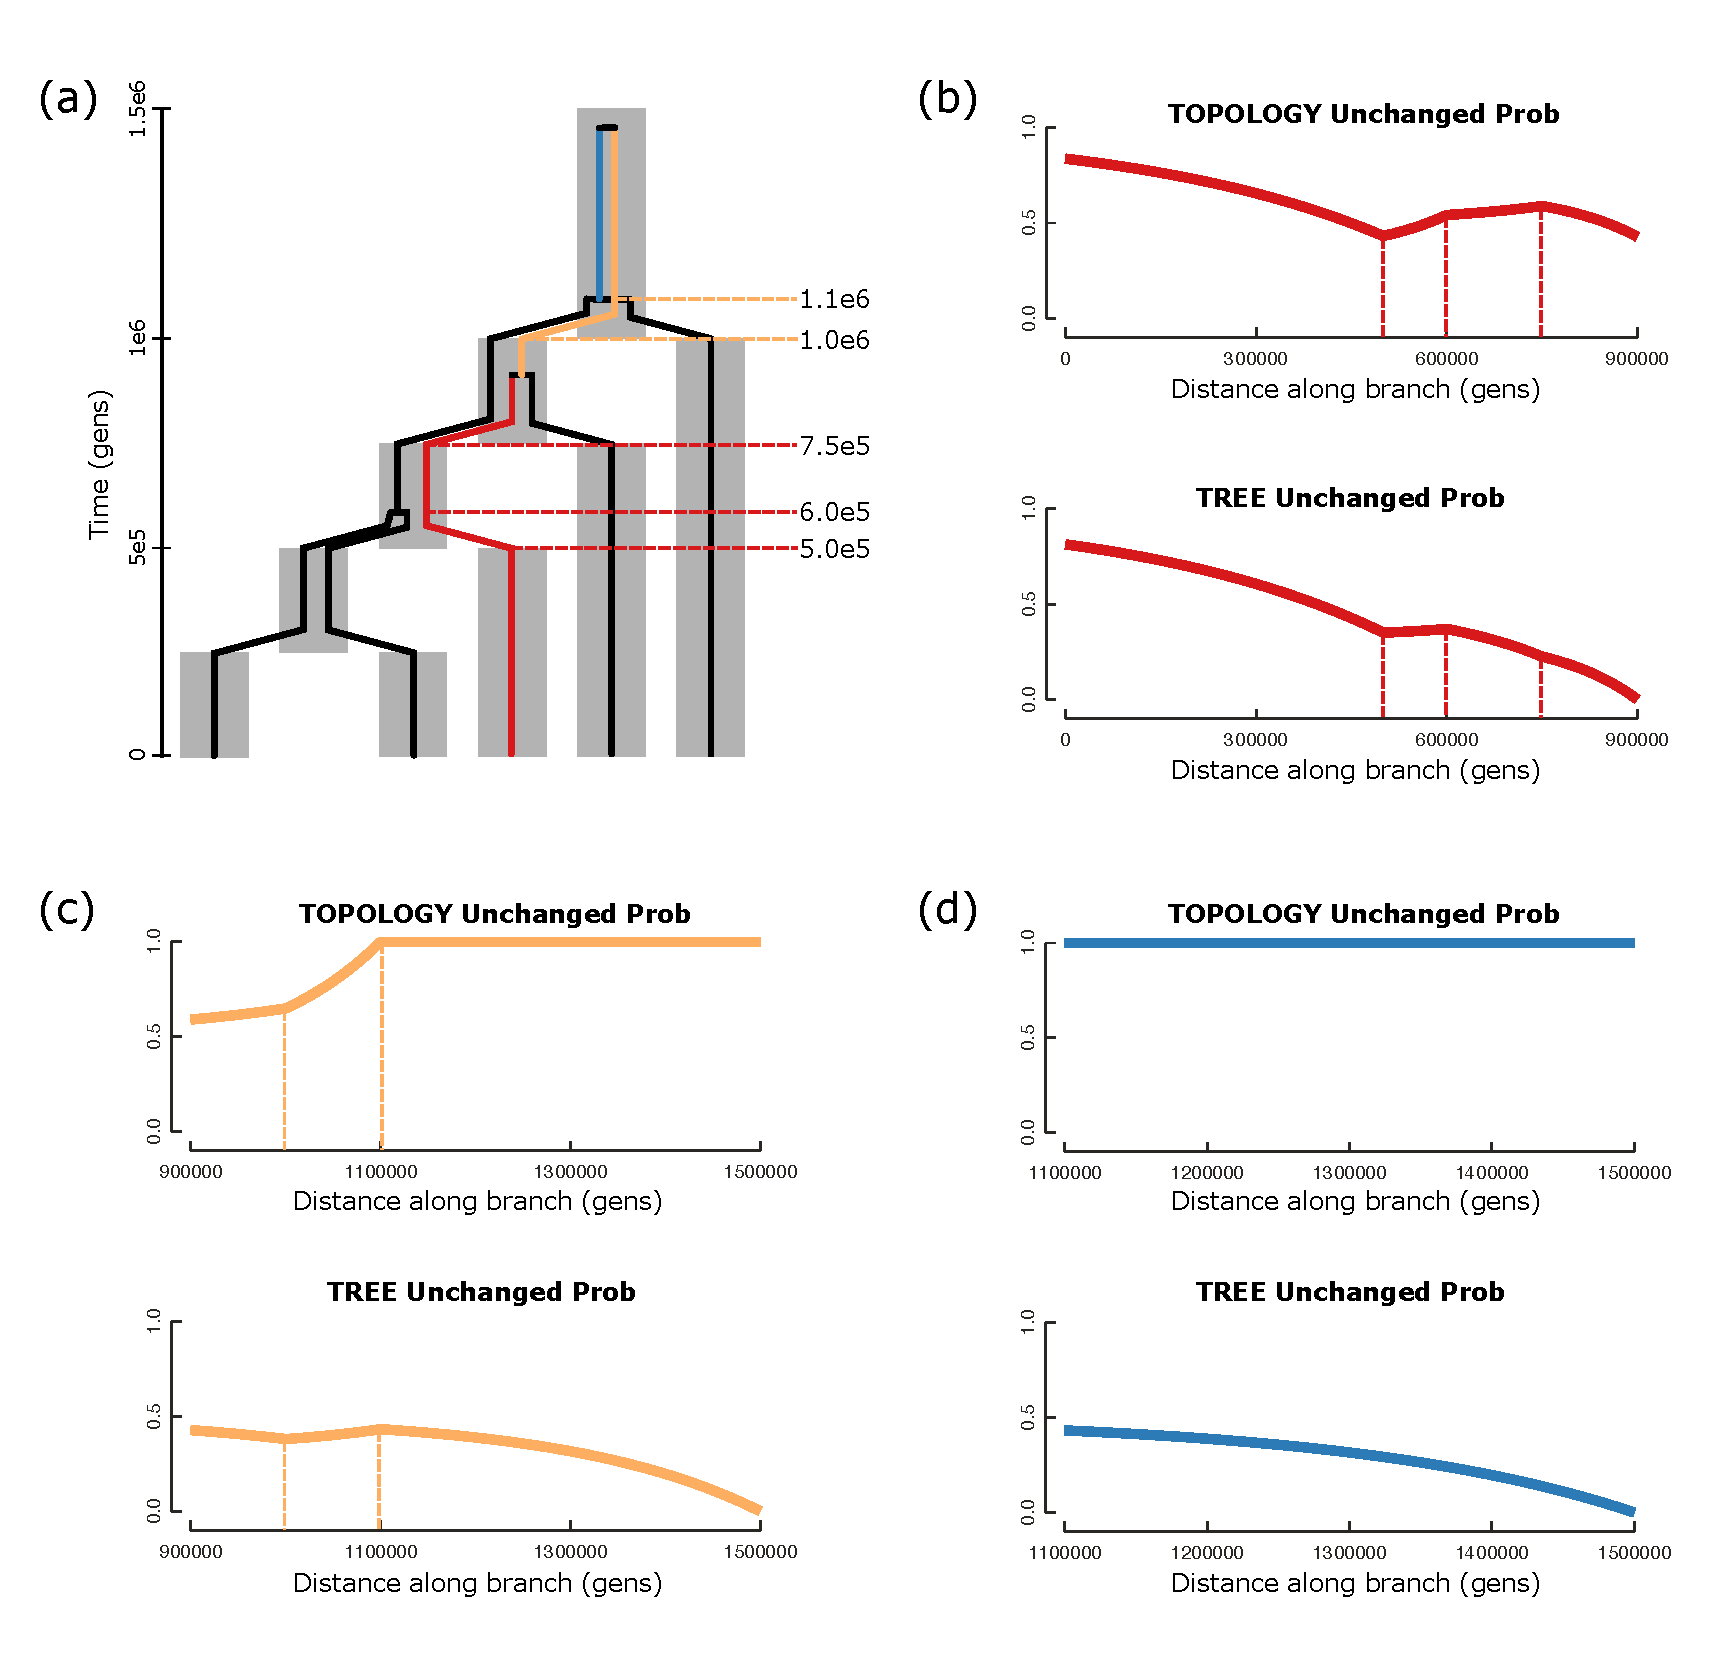
\includegraphics[width=0.9\textwidth]{figures/Fig4-bt_prob.pdf}
%	\caption{Probability that the topology and the tree remain unchanged, given a recombination event at a specific time on a specific branch. The species tree (a) was arbitrarily parameterized as being unbalanced with 5 tips, having internode distances of 2.5e5, and having constant Ne of 2e5. The embedded genealogical tree was randomly generated by \emph{ipcoal} using MSC probabilities. We selected three branches, indicated by three different colors, across which we calculated the probability that the topology would remain unchanged and the tree would remain unchanged if a recombination event were to occur at each time point on the branch (b-d). Dashed lines indicate the beginning and ending times of different intervals on each branch -- that is, either a relevant species tree divergence event or genealogy coalescence event.}
%	 \label{fig:fig3}
%\end{figure}

% This was tested for demographic models with different numbers of lineages;
% different numbers of samples among lineages; 
% and with different MSC model parameters, with the goal of representing scenarios
% spanning from population genetic to deeper-scale phylogenetic datasets. All
% datasets show nearly perfect matching between expected and simulated waiting 
% distances (Fig.~\ref{fig:fig-validation}). 

\subsection{Validation}


\begin{figure}[tp]
	\centering
	%\fbox{\rule[-.5cm]{4cm}{4cm} \rule[-.5cm]{4cm}{0cm}}
	% 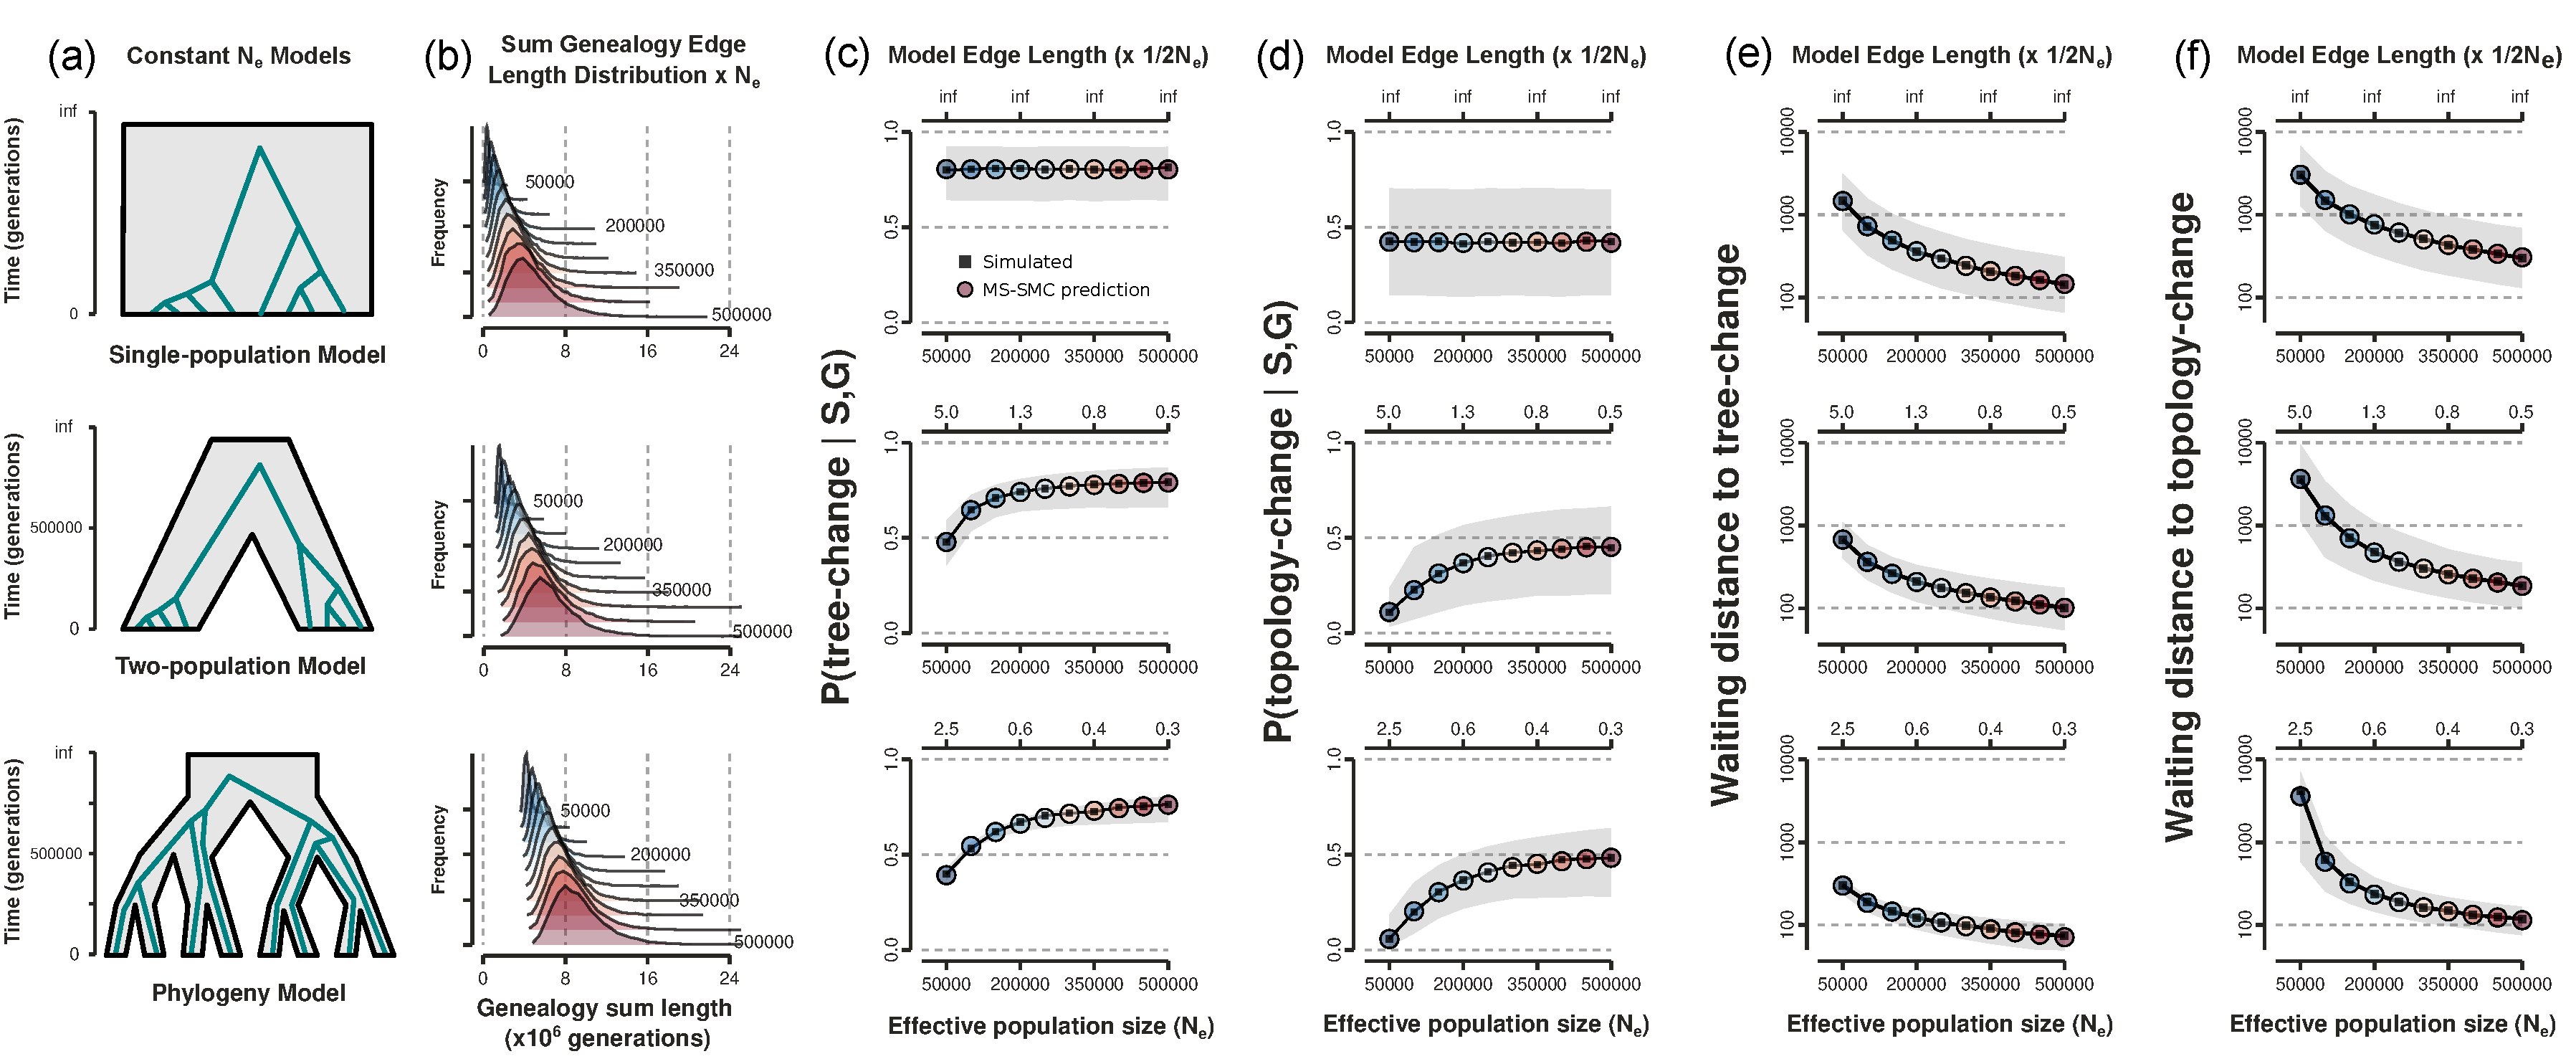
\includegraphics[width=0.99\textwidth]{figures/current/Fig5-validation-sims.pdf}
	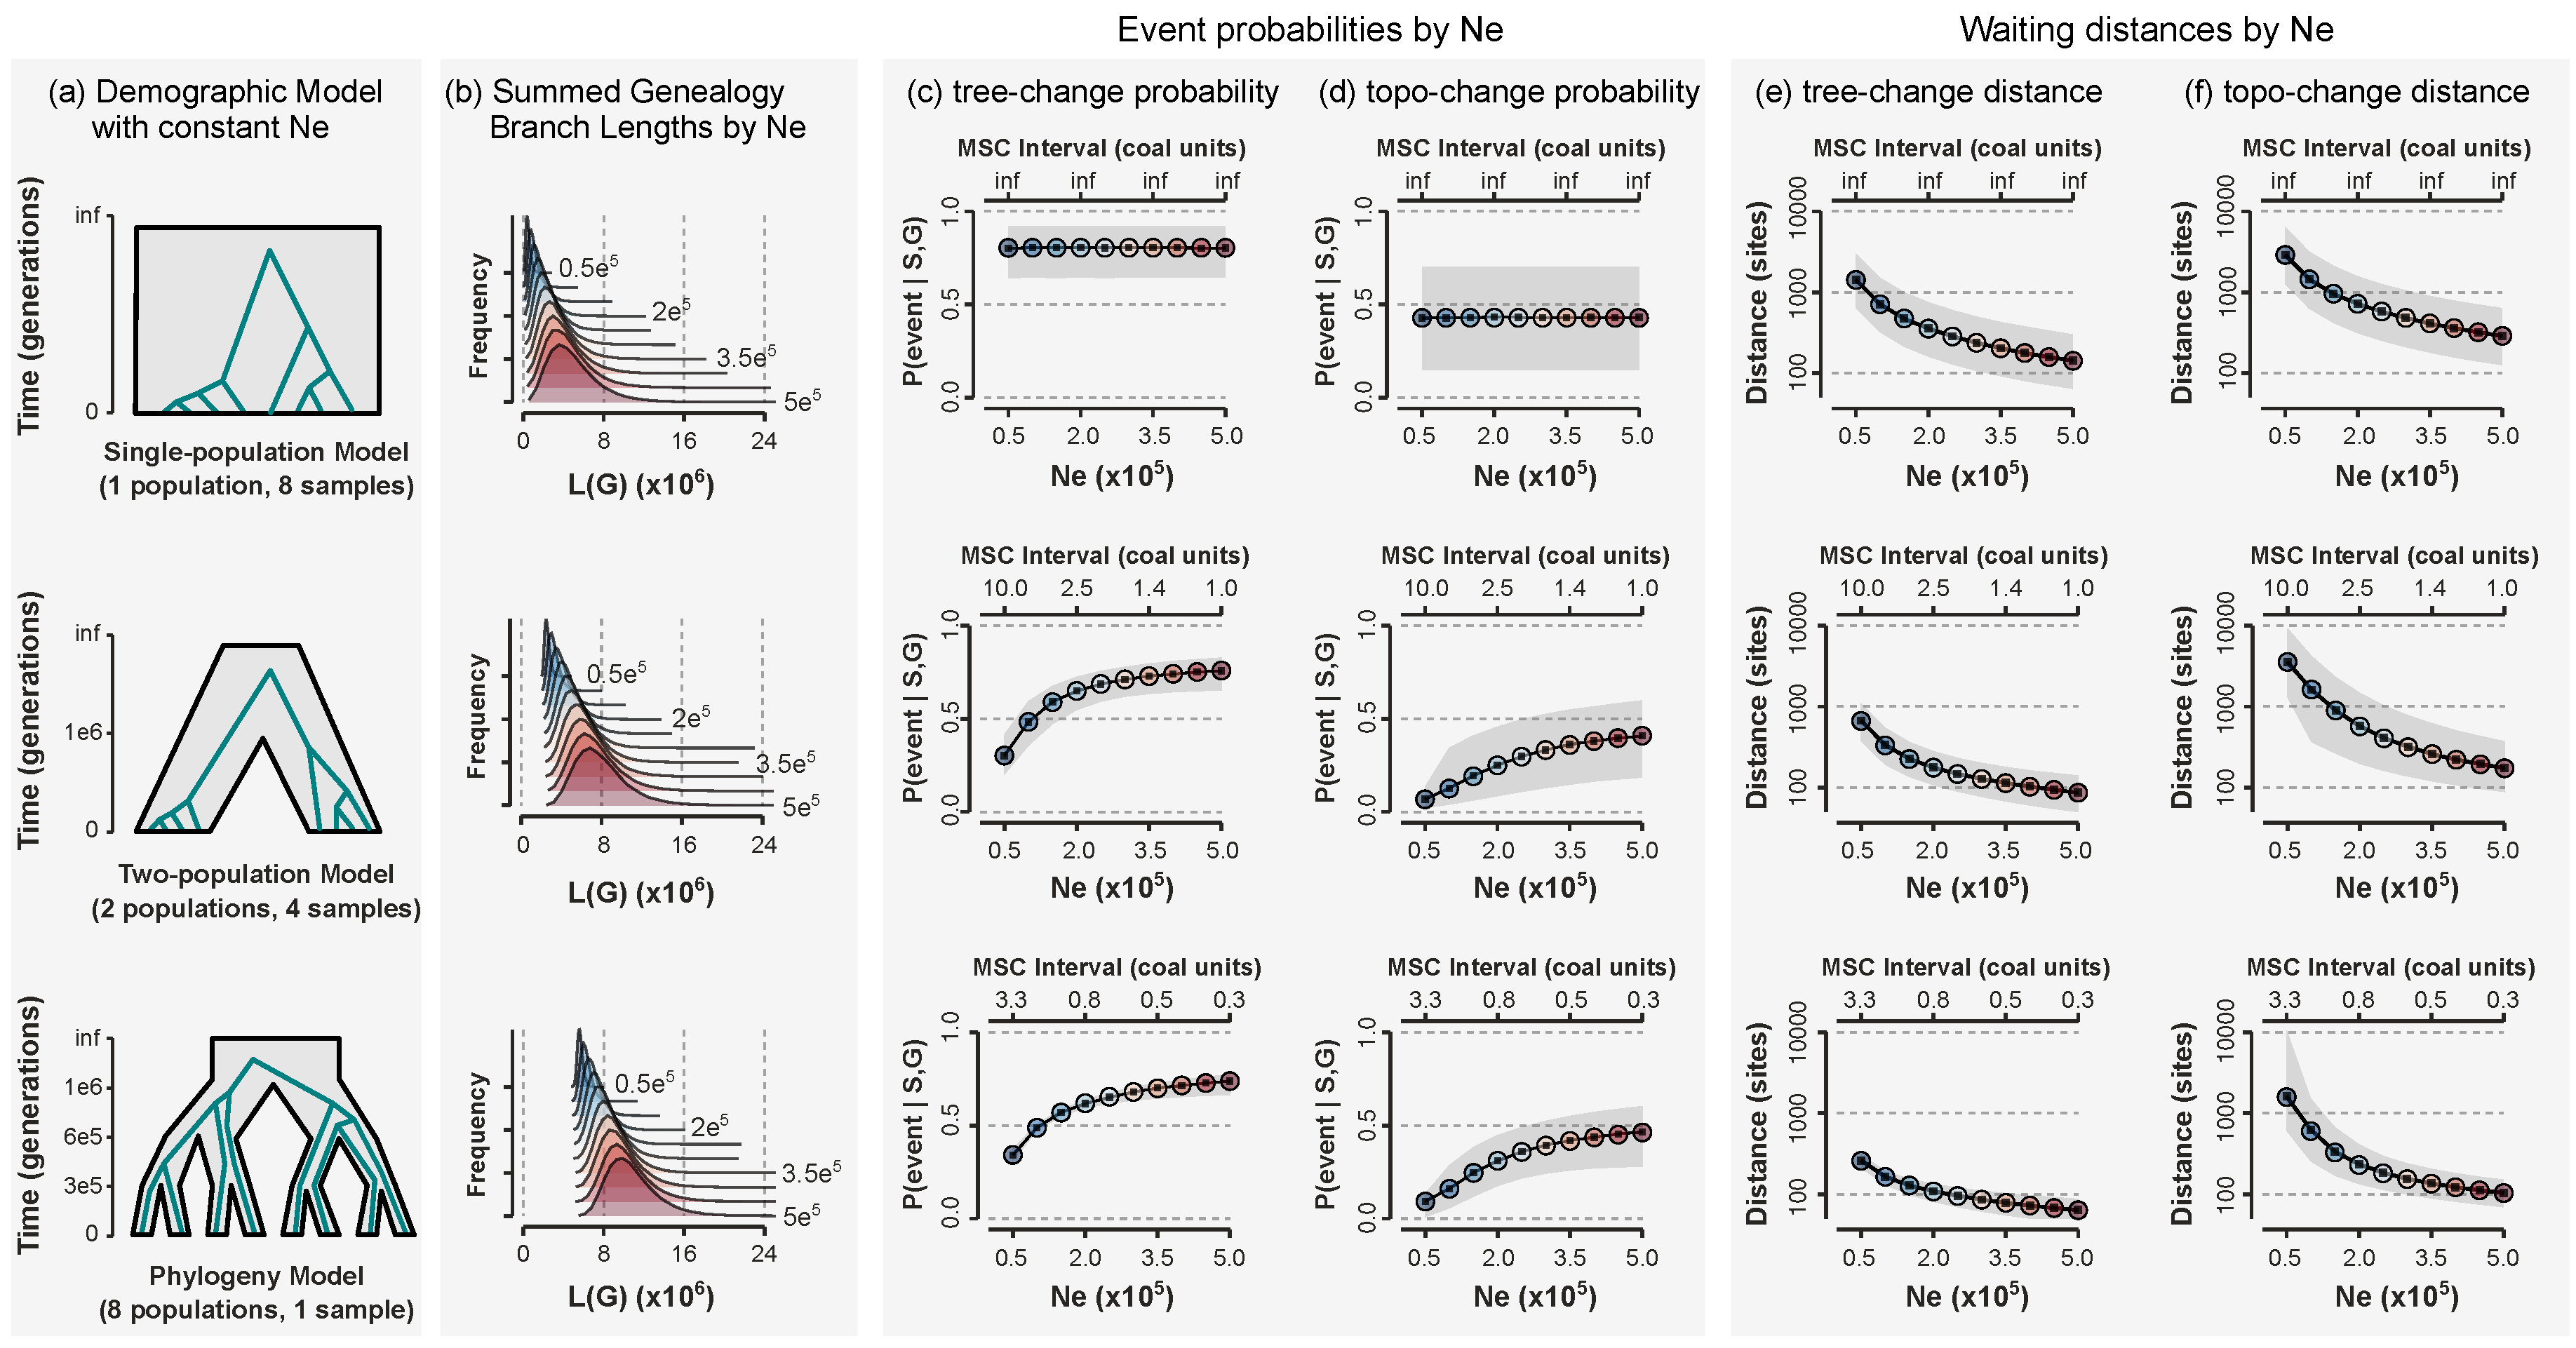
\includegraphics[width=0.99\textwidth]{figures/current/Fig5-validation-sims-NEW4.pdf}
	\caption{
		MS-SMC predictions validated against coalescent simulations.
		(a) Results are shown for three models containing 1, 2, or 8 
		populations. % among which genealogies for 8 samples were embedded. 
		For each model, 10\textcolor{red}{0}K tree sequences were simulated for 10 different
		constant $N_e$ values between 50K and 500K. 
		(b) The distributions of summed edge lengths of the first genealogy in 
		each tree sequence. 
		(c-d) The mean frequency (black square) with which the first observed 
		recombination event was a tree-change (c) or topology-change (d) in a 
		simulated tree sequence, and the mean (colored circle) and 95\% CI 
		(grey fill) of the predicted probability of tree or topology-change 
		calculated from the first embedded genealogy in each tree sequence. 
		Probabilities are constant with respect to $N_e$ in the single population
		%model, but vary in models with population structure
		model but vary in models with population structure
		%% ^removing all commas like this whenever I notice complex sentences beginning
		%% with an independent clause. (Or occassionally keeping the comma and just 
		%% adding a subject to the second clause.)
		(also shown with respect to species tree interval lengths in 
		coalescent units, across the top axis).
		% The probabilities of tree-change or topology-change are 
		% constant with respect to N$_e$ in a single population model, 
		% but vary in models with population structure (also shown with respect to 
		% species tree interval lengths in coalescent units, across the top axis). 
		(e-f) The mean waiting distance (black square) until the first observed 
		tree-change (e) or topology-change (f) in a simulated tree sequence, and the mean 
		(colored circle) and 95\% CI (grey fill) of predicted waiting distances calculated
		using the first embedded genealogy in each tree sequence.
		 % under the MS-SMC. 
		% Predicted Predicted waiting distances Waiting distances between tree or topology-change events exhibit 
		% less variance for a given $N_e$ value in models with population structure. 
		% The MS-SMC calculated waiting distance expectations match very closely to simulated values.
		% , however,
		% whereas the tree-change waiting distance is exact, the the topology-change waiting distance exhibits slight bias at very low 
		% N$_e$ values.
	}
	\label{fig:fig-validation}
\end{figure}


% we simulated data under 3 models to validate our results
To validate our analytical solutions for the probabilities of different 
recombination event outcomes and their associated waiting distances, 
we compared predictions of the MS-SMC with results from stochastic 
coalescent simulations. 
We set up three scenarios with increasing amounts of population structure: 
a single-population model, a two-population model, and an 8-tip phylogeny model
(Fig.~\ref{fig:fig-validation}a). 
All analyses used a constant per-site per-generation recombination rate of 
2e-9 and simulated tree sequences using the coalescent with recombination 
(i.e., the "hudson" ancestry model in msprime as opposed to the "smc\_prime" model, 
which is an approximation), %unless specified, 
and the argument 
"record\_full\_arg=True" (to retain records of invisible recombination events). 
For each model we simulated genealogies for the same total number of samples
(8, unless specified), divided evenly among lineages when models 
include multiple populations (Fig.~\ref{fig:fig-validation}a). 
% When N$_e$ is low, 
% population structure is expected to have large effects, whereas when N$_e$ is 
% high, barriers imposed by population structure are expected to have 
% limited effects.


% results are composed of L, P, and L x P, which are calculated from sims in this way...
The exponential rate parameter ($\lambda$) for a probability distribution of waiting distances 
is a product of the per-site per-generation recombination rate ($r$), the sum 
of edge lengths on the current genealogy ($L(\mathcal{G})$), and the probability 
($\mathbb{P}$) of the specified event type (equations 9, 10, and 14). 
Across the three models examined, $r$ remains constant, but both $L(\mathcal{G})$ 
and $\mathbb{P}$ can vary due to population structure, where the effect of 
structure is scaled by $N_e$. 
Therefore, we examined $L(\mathcal{G})$, $\mathbb{P}$, and the expected waiting 
distance calculated from their product, for each demographic model across a range 
of $N_e$ values (50K -- 500K; Fig.~\ref{fig:fig-validation}b-f). 
% 
% NEW TEXT DESCRIBING THE SKIP-FIRST-TREE APPROACH
\textcolor{red}{At each value of $N_e$ we simulated 100K tree sequences for each
demographic model.}

\textcolor{red}{
% To validate the accuracy of MS-SMC our analytical method we compared the observed 
% event probabilities and waiting distances in simulated tree sequences to 
% analytical expectations computed under the MS-SMC. 
Each simulated tree sequence
contains a series of trees and intervals representing stochastic outcomes of
the coalescent with recombination. Over many replicates, we expect the mean
waiting distances until the first tree and topology-change events in simulations 
to match the predicted waiting distances estimated under the MS-SMC, computed
from only observing the starting tree in each tree sequence.
(Note that to avoid any potential bias associated with the first tree interval 
in simulated tree sequences we actually advanced to the first tree after the 
first topology-change event to serve as the starting tree in all analyses.) 
To measure tree and topology-change waiting distances in tree sequences we 
recorded the sum length of the interval that includes the starting tree, and any 
subsequent intervals in which no tree-change occurred, or no topology-change 
occurred, respectively. To measure the probability of each event type in simulations
we recorded which event type (including no-change events) was the first to occur 
after the starting tree in each tree sequence. 
The MS-SMC probabilities of each event type were computed in \emph{ipcoal} by 
embedding the starting tree of each tree sequence into the parameterized MSC model.
Expected waiting distances under the MS-SMC were computed as 1 over the product 
of the event probabilities, $r$, and $L(\mathcal{G})$ of the starting tree.
}
% THIS TEXT WAS REPLACED BY THE BLOCK ABOVE
\textcolor{red}{\sout{For each value of $N_e$, 10K tree sequences were simulated that
included at least one topology-change event.
The empirical probabilities of tree-change and topology-change events were simply 
calculated as the mean observed frequency at which the first recombination event 
in each tree sequence was a tree or topology change. 
Similarly, empirical waiting 
distances were measured as the mean distance until the first observation of 
each event type. These simulated expectations were then compared with analytical
expectations computed under the MS-SMC, where probabilities and waiting distances 
were based only on the embedding of the first genealogy from each tree sequence 
into an MSC model parameterized to the specific constant $N_e$ value. 
}}


% Given each starting genealogy,
% the probability of each event type, and the expected waiting distance to that event
% type, were calculated under the MS-SMC. To compare this with the result of a 
% simulated coalescent with recombination process, we recorded the waiting distance 
% until each recombination event type first occurred in each tree sequence, and 
% also the frequency at which each event type occurred as the first event in a 
% tree sequence, as a measurement of its empirical probability.

% L and P have opposing effects on waiting distances given Ne
Population structure enforces a 
\textcolor{red}{limit on the minimum length
\sout{lower limit on the length}} of coalescent 
times by requiring that genealogies can be embedded in a species tree.
% This has an effect on $L(\mathcal{G})$ %at both low and high N$_e$
% of shifting both its minimum and mean 
This has the effect of shifting both the minimum and mean of 
$L(\mathcal{G})$ higher 
\textcolor{red}{across all values of $N_e$}
(Fig.~\ref{fig:fig-validation}b). 
Because the per-generation recombination rate interacts with
$L(\mathcal{G})$ (the opportunity over which recombination can occur) to
determine the frequency of recombination, larger $L(\mathcal{G})$ induced
by population structure will tend to decrease waiting distances between 
recombination events, all else being equal. 
% 
% \textcolor{red}{This is clear in the case of the single population model, where 
% changing Ne has no effect on tree or topology-change event probabilities 
% (Fig. 5c-d) and thus the relationship between Ne and waiting distances 
% (Fig. 5e-f) is determined solely by the effect of Ne on genealogy edge lengths. 
% However, this is not the case for the population structured models.
% Instead, Ne has a direct effect on event probabilities in MSC models, 
% where it scales the coalescent rate and thus the extent to which barriers
% between lineages constrains coalescent events between them (Fig.).
% When Ne is very low
% }
% 
However, all else does not remain equal.
% 
\textcolor{red}{
Instead, population structure in MSC models has a simultaneous opposing effect
of increasing the mean waiting distance to tree or topology change events by 
affecting the event probabilities
(Fig.~\ref{fig:fig-validation}c-d).
This is most clear at low values of $N_e$, where shorter coalescent times are
less likely to span the barriers between lineages in an MSC model. 
This has the effect of increasing the probability of no-change events
relative to tree or topology-change events. By contrast, when $N_e$ is high the 
barriers in an MSC model have little effect on coalescence probabilities, and 
the tree and topology-change event probabilities in MSC models converge towards 
those seen in the single population model
(Fig.~\ref{fig:fig-validation}c-d). 
% 
This highlights the relationship between MSC model parameters and the waiting 
distances between different recombination event types. In MSC models, waiting
distances to the three different recombination event types can vary as a 
consequence of the model parameters' effects on $L(\mathcal{G})$ and $\mathbb{P}$, 
whereas in a single population model each waiting distance is simply scaled 
by $L(\mathcal{G})$.
}
% 
% 
\textcolor{red}{\sout{
Population structure has a simultaneous opposing effect on waiting distances
by decreasing the probability of tree or topology changes 
% ($\mathbb{P}$; Fig.~\ref{fig:fig-validation}c-d), 
especially at low $N_e$ values,
where species tree constraints can make tree or topology changes unlikely
to occur. This is a stark difference between the MS-SMC framework and a 
single population model: the probability of a tree- or topology-change 
% accompanying a recombination 
event is strongly associated with $N_e$ in the former but not affected 
at all in the latter. 
%% Capitalization after a colon? APA says yes, Chicago says no. IMO No.
%% (but I do think a colon is more appropriate than a semicolon here)
Consequently, the waiting distances between each event type in MSC models 
% (Fig.~\ref{fig:fig-validation}e-f)
represent a balance 
of the positive and negative effects of population structure on 
$L(\mathcal{G})$ and $\mathbb{P}$, respectively.
}}

% Analytical predictions are very accurate, even better given SMC' approximation.
Our analytical predictions under the MS-SMC converge accurately on 
the mean results from stochastic coalescent simulations 
(Fig.~\ref{fig:fig-validation}c-f). 
% Examining the relationship between MSC model parameters and expected 
% waiting distances also reveals ...
Moreover, by examining the variance in these predictions with 
respect to MSC model parameters we further gain insights into 
the information contained in spatial genealogical patterns.
% In a single population, the probability of a tree or topology change event
% is not only invariant with respect
For example, in the single population model there is high variance 
in both the probabilities of tree and topology changes, as well as in genealogy
lengths, at any given $N_e$ value. Consequently, waiting distances also 
exhibit high variance. Although waiting distances correlate with population $N_e$ 
in this model, the differences in mean waiting distances are small relative to the variance. 
By contrast, multispecies models exhibit much less variance in predicted probabilities 
of tree or topology changes given a set of MSC model parameters 
(Fig.~\ref{fig:fig-validation}c-d) and also exhibit less variation in genealogy
lengths. This leads to a stronger relationship between MSC model parameters and 
expected waiting distances (Fig.~\ref{fig:fig-validation}e-f), such that models
with different parameters have less overlap in waiting distance expectations.
\textcolor{red}{
Overall, this demonstrates that estimations of tree- and topology-change
waiting distances calculated under the MS-SMC are accurate, and contain 
% significant
information for inferring population demographic parameters.
}
\textcolor{red}{\sout{
Overall, this suggests that tree- and topology-change distances may contain more 
information in MSC models than in single population models.
}}
% ; information that
% can be used for inferring demographic model parameters from waiting distances 
% in ARGs, or for inferring ARGs in the context of demography.

% The probabilities of tree or topology change events are highly variable in 
% the single population model, and constant with respect to $N_e$, whereas these probabilities exhibit 
% little variation for any given constant $N_e$-valued MSC model
% (Fig.~\ref{fig:fig-validation}c-d). This makes sense, considering 
% that genealogies in the latter models are constrained, especially
% when $N_e$ is low. This similarly leads to less variation in 
% expected waiting distances between tree or topology changes in 
% MSC models (Fig.~\ref{fig:fig-validation}e-f).
% where 
% genealogies are not constrained by population structure, and 
% thus exhibit no relationship with $N_e$. 
% By contrast, multispecies models exhibit much less variation
% in the probabilities of tree or topology change events given the 
% MSC model parameters (Fig.~\ref{fig:fig-validation}c-d). This makes
% sense, since the MSC model will constrain the types of genealogies
% that can be observed.
% Waiting distances to tree or topology-change events exhibit much less 
% variance for a given in MSC models than in the 
% The variance in waiting distance expectations at any examined $N_e$ value 
% are narrower in models with greater population structure, such as the 
% 8-population phylogeny model, than for the less structured models.
% Similarly, the magnitude of differences are also greater between waiting 
% distances given different N$_e$ in more highly structured MSC models.
% This suggests that tree and topology-change information is more informative 
% about demographic parameters (and vice versa) when population structure 
% is present. 
% We examine this further below to explore a likelihood framework 
% for MSC inference based on waiting distance expectations.

% As expected, 
% solutions for the probabilities of each event type (Fig.~\ref{fig:fig-validation}c-d), 
% and for waiting distances to tree-change events (Fig.~\ref{fig:fig-validation}e),
% appear as exact solutions, whereas the expected waiting distance to a topology-change
% event shows some bias at the lowest $N_e$ values (Fig.~\ref{fig:fig-validation}f). 

% waiting distances until tree or topology-change events decrease as
% values of N$_e$ increase, and topology-change waiting distances are always larger
% than tree-change waiting distances. 

\subsection{Bias in waiting distance estimation}
Estimated waiting distances under the MS-SMC harbor two potential sources of bias, 
the first stemming from assumptions of the SMC' approximation, and the second from 
the approximate nature of waiting distance estimation for topology-change events. 
We examined both of these sources of error through comparison to stochastic simulations
and found that their effects are generally small, and that multispecies models exhibit 
a similar magnitude of error as single population coalescent models 
% Supplementary Materials; Fig.~\ref{fig:figS-bias-smc}, Fig.~\ref{fig:figS-bias-topo}).
\textcolor{red}{
(see "Investigating bias" section in Supplementary Materials; 
Fig.~\ref{fig:figS-bias-smc}, 
Fig.~\ref{fig:figS-bias-topo-first}, 
Fig.~\ref{fig:figS-bias-topo-last}).
The SMC' approximation introduces very little bias to MS-SMC estimates of 
tree-change waiting distances across all scenarios examined, and only 
significantly biases topology-change waiting distance estimates in the 
"species tree" demographic model scenario at very low $N_e$ values -- a 
scenario where genealogical discordance becomes very unlikely. 
This scenario is also most affected by the other source of bias, as
it exhibits greatest variance in genealogy branch lengths among
intervals between topology-change events. For both sources of bias, 
we show that error is greatly reduced by simply increasing the number
of genomes sampled per lineage.
\sout{
The SMC’ approximation contributes most error, leading to slight under-estimation of waiting distances
that is most observable when variance in waiting distances is high, as with topology-change waiting dis-
tances in models with low $N_e$. Future work can likely find a correction for this bias.
}
}

% when the probability
% of topology-change events becomes very low. We show that by simply add

% )
% The approximate nature of waiting ditsance estimation to topology-change events 


% Both sources of error have greatest impact in species tree models when Ne
% is low, such that topology-change
% }
% The SMC' approximation contributes the greatest error in all models, leading to 
% a slight 
% \textcolor{red}{over-estimation}
% \textcolor{red}{\sout{under-estimation}}
% of waiting distances. This is most observable when variance
% in waiting distances is high, as with topology-change waiting distances in 
% \textcolor{red}{highly structured} models with low $N_e$. 
% \textcolor{red}{In other words, the MS-SMC model will exhibit greatest error
% in demographic models that exhibit little to no gene tree discordance.}
% % thus not highly suitable for analyzing data that lacks gene tree conflicts.
% Future work could seek to find a correction for this bias.

% \subsection{\textcolor{red}{Waiting Distances to Topology-changes}}
% ...
% Drosophila example five species tree and recombination rate. If we sample a 
% single phased genome per species the estimated waiting distance is XX. If
% we sample two phased genomes per species this decreases to XX. ...
% ...
% SImilar to our book chapter we could report that topology-change distances 
% are generally very short for phylogenetic-scale datasets, suggesting that 
% concatalescence is a big problem... This could involve listing examples of 
% studies that used large sliding windows, ...
% The MS-SMC model can provide insights into the extent of gene tree 
% estimation error in studies of genome-wide phylogenetic patterns. For example,
% table X lists a series of 
% Given a species tree of different sizes, and with different number of 
% sampled genomes per species, and for different 

\subsection{
\textcolor{red}{A Likelihood-based Framework for Evaluating Waiting Distances}
}

\textcolor{red}{
\sout{
Based on the expectation that waiting distances are informative 
about MSC model parameters, we developed a maximum likelihood framework 
for inferring MSC model parameters from observed waiting distances between
tree and/or topology change events. Here, we apply this method using the 
true distances between events in simulated ARGs, however, it could similarly
be applied to inferred distances between events in an ARG proposed from 
sequence data.
}
}
% \subsection{\textcolor{red}{Likelihood of a Species Tree Given an ARG}}
\textcolor{red}{
% this first paragraph is repetitive with the one above...
The MS-SMC is a statistical model of the waiting distances between different
types of genealogy changes in an ARG, given a parameterized MSC model. 
Since waiting distances between recombination events follow an exponential 
distribution, we can use the exponential probability density (equation 8) 
as the likelihood function to assess observed (or estimated) waiting
distances in an ARG, by modeling the probability of these waiting distances
as a function of demographic model parameters.
% 
% model the joint probability of observed 
% (or estimated) waiting distances in an ARG.
% In the case of tree and topology-change waiting distances, 
% this likelihood function is dependent on MSC model parameters, and thus
% we expect that it can provide information for estimating these parameters.
We propose that applications of this approach can provide 
improvements to ARG and demographic model inference methods. Below, we
describe and demonstrate one such application.
}
% To demonstrate one such application, we developed a likelihood framework
% for fitting MSC model parameters to observed waiting distances
% between tree-change and/or topology-change events in simulated ARGs.
% 
% Here, to explore the potential of this approach, we developed a 
% \textcolor{red}{rudimentary} maximum likelihood framework 
% \textcolor{red}{as a proof-of-concept} for the latter: 
% we apply the MS-SMC to fit MSC model parameters to observed distances
% between tree-change and/or topology-change events in simulated ARGs.
% }
% It could similarly be applied to ARGs inferred 
% from sequence data. 
% 
% , by incorporating information from the 
% likelihood of observed tree and topology-change waiting distances 
% given a parameterized MSC model; and (2) to 
% in which MSC model parameters can be fit from waiting distances in ARGs, 
% 
% Based on the expectation that waiting distances are informative about 
% MSC model parameters, we developed a maximum likelihood framework for inferring 
% MSC model parameters from observed waiting distances between tree and/or topology 
% change events. Here, we apply this method using the true distances between 
% events in simulated ARGs, however, it could similarly be applied to inferred 
% distances between events in an ARG proposed from sequence data. 
% 

\textcolor{red}{
Given one or more ARGs each composing a sequence of genealogies and
their interval lengths in a genome, 
a subset of genealogies and intervals can be extracted that represent 
the combined intervals between a specific type of event
(Fig.~\ref{fig:likelihood-calculation}a).
For example, $\boldsymbol{\mathcal{G}_g}$ = ($\mathcal{G}_1, \mathcal{G}_j, ...$)
can represent
the subset of genealogies that occur between tree-change events
and $\boldsymbol{X_g}$ = ($\sum_{i=1}^j x_i, \sum_{i=j}^{k} x_i, ..., $)
the summed lengths of intervals between tree-change events
(Fig.~\ref{fig:likelihood-calculation}b-c).
The same can be done for topology-change events.
Given a parameterized MSC model and recombination rate
we can then obtain a set of exponential rate parameters
$\boldsymbol{\Lambda_g} = (\lambda_1, \lambda_j, ...)$ for the waiting distance 
until the next tree-change for each genealogy in G$_g$ 
(equation 10; Fig.~\ref{fig:likelihood-calculation}d).
% 
Finally, using the exponential probability density function,
the likelihood of the MSC model parameters is calculated as the
product of the probability densities for each waiting distance
in X$_g$, evaluated using the corresponding rate parameters in 
$\boldsymbol{\Lambda_g}$
% of each observed waiting distance in X$_g$
% can be calculated from the exponential probability density function 
% using the rate parameters in $\Lambda_g$
(Fig.~\ref{fig:likelihood-calculation}e).
% The closer the MSC model paramaters are to the true values, the closer
% the predicted waiting distances should be to the observed data.
Maximum likelihood optimization of the model parameters can be achieved
by identifying the set of parameters -- affecting $\boldsymbol{\Lambda_g}$ -- that
maximize the likelihood function, which quantifies the probability of 
the observed data given the model.
% 
% A maximum likelihood optimization of MSC model parameters can be obtained
% by searching for the set of parameters -- which affect $\Lambda_g$ -- 
% that maximize the summed log-likelihood of the observed data.
}

% OLD COPY 
\textcolor{red}{
\sout{
Given one or more ARGs each composing a sequence of genealogies 
G = ($\mathcal{G}_1, \mathcal{G}_2, ..., \mathcal{G}_n$) and 
their interval lengths in the genome X = ($x_1, x_2, ..., x_n$),
a subset of genealogies can be extracted that represent the unique 
trees between tree-change events, 
G$_g$ = ($\mathcal{G}_1, \mathcal{G}_j, ...$), and 
waiting distances can be measured as the summed interval lengths between 
these trees, 
X$_g$ = ($\sum_{i=1}^j x_i, \sum_{i=j}^{k} x_i, ..., $).
The same can be done for topology-change events.
Given a parameterized species tree, $\mathcal{S}$ and recombination 
rate, $r$, we can then obtain a sequence of exponential rate parameters
$\Lambda_g = (\lambda_1, \lambda_j, ...)$ corresponding to each genealogy
in G$_g$ (equation 10).
The likelihood of each observed waiting distance in X$_g$
can then be calculated from the exponential probability density 
function with rate parameters from $\Lambda_g$. 
The maximum likelihood solution is found by searching for the
set of MSC model parameters -- which affect $\Lambda_g$ -- 
that maximize the summed log-likelihood of the observed waiting distances.
}}

\begin{figure}[tp]
	\centering
	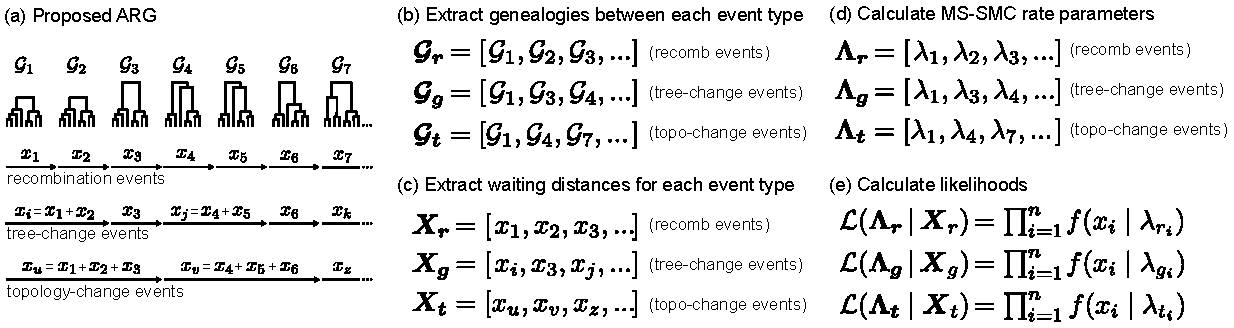
\includegraphics[width=0.99\textwidth]{figures/current/Fig6-ARG-likelihood-steps-full.pdf}
	\caption{
	\textcolor{red}{	
		A likelihood framework for fitting MSC model parameters from waiting distances
		between categorical types of recombination events in an ARG.
		(a) An ARG represents a sequence of genealogies ($\mathcal{G}$) and their
		interval lengths ($x$) over a genomic region. Intervals can be delimited 
		by all recombination events, or by a subset representing only tree-change, 
		or only topology-change events.
		(b) The set of genealogies ($\boldsymbol{\mathcal{G}}$) occurring between
		each event type can be extracted, and similarly, 
		(c) the set of associated interval lengths ($\boldsymbol{X}$) between
		each event type can be extracted.
		(d) A set of exponential rate parameters ($\boldsymbol{\Lambda}$) can 
		then be estimated under the MS-SMC for the waiting distance until 
		each type of recombination event, for each genealogy, given its 
		embedding in a parameterized MSC model
		($\mathcal{S}$) and the recombination rate ($r$).
		(e) Using the exponential probability density function, the likelihood 
		of the MSC model parameters is calculated as the product of the 
		probability densities for each waiting distance in $\boldsymbol{X}$,
		evaluated using the corresponding rate parameters in 
		$\boldsymbol{\Lambda}$.
	}}
	\label{fig:likelihood-calculation}
\end{figure}


\textcolor{red}{\sout{
We first implemented this approach for a simple two-population model with 
constant $N_e$=200K and a population divergence at 500K generations. 
We simulated 100 independent ARGs, each 100Kb in length, using $r$=2e-9, 
and we sampled four haplotypes per population. This 
yielded 51,487 tree-change events, with mean length 194bp, and 25,446 
topology-change events, with mean length 393bp. To examine the likelihood
surface, we calculated the log-likelihood of joint parameters for $N_e$ and $r$, 
while keeping a fixed divergence time parameter, over a grid search of 41
evenly spaced values from $r$=1e-9 to 3e-9 and 
$N_e$=50K to 800K.
}}


\begin{figure}[p]
	\centering
	%\fbox{\rule[-.5cm]{4cm}{4cm} \rule[-.5cm]{4cm}{0cm}}
	% 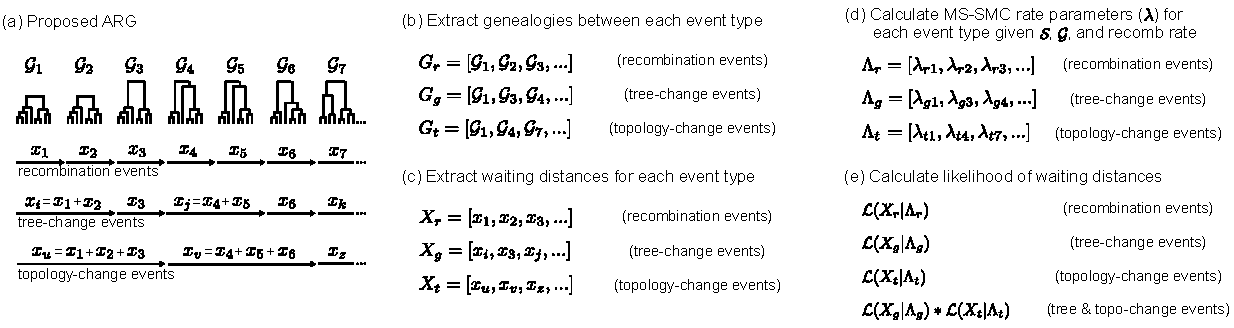
\includegraphics[width=0.99\textwidth]{figures/FigX-ARG-likelihood-wide.pdf}
	% 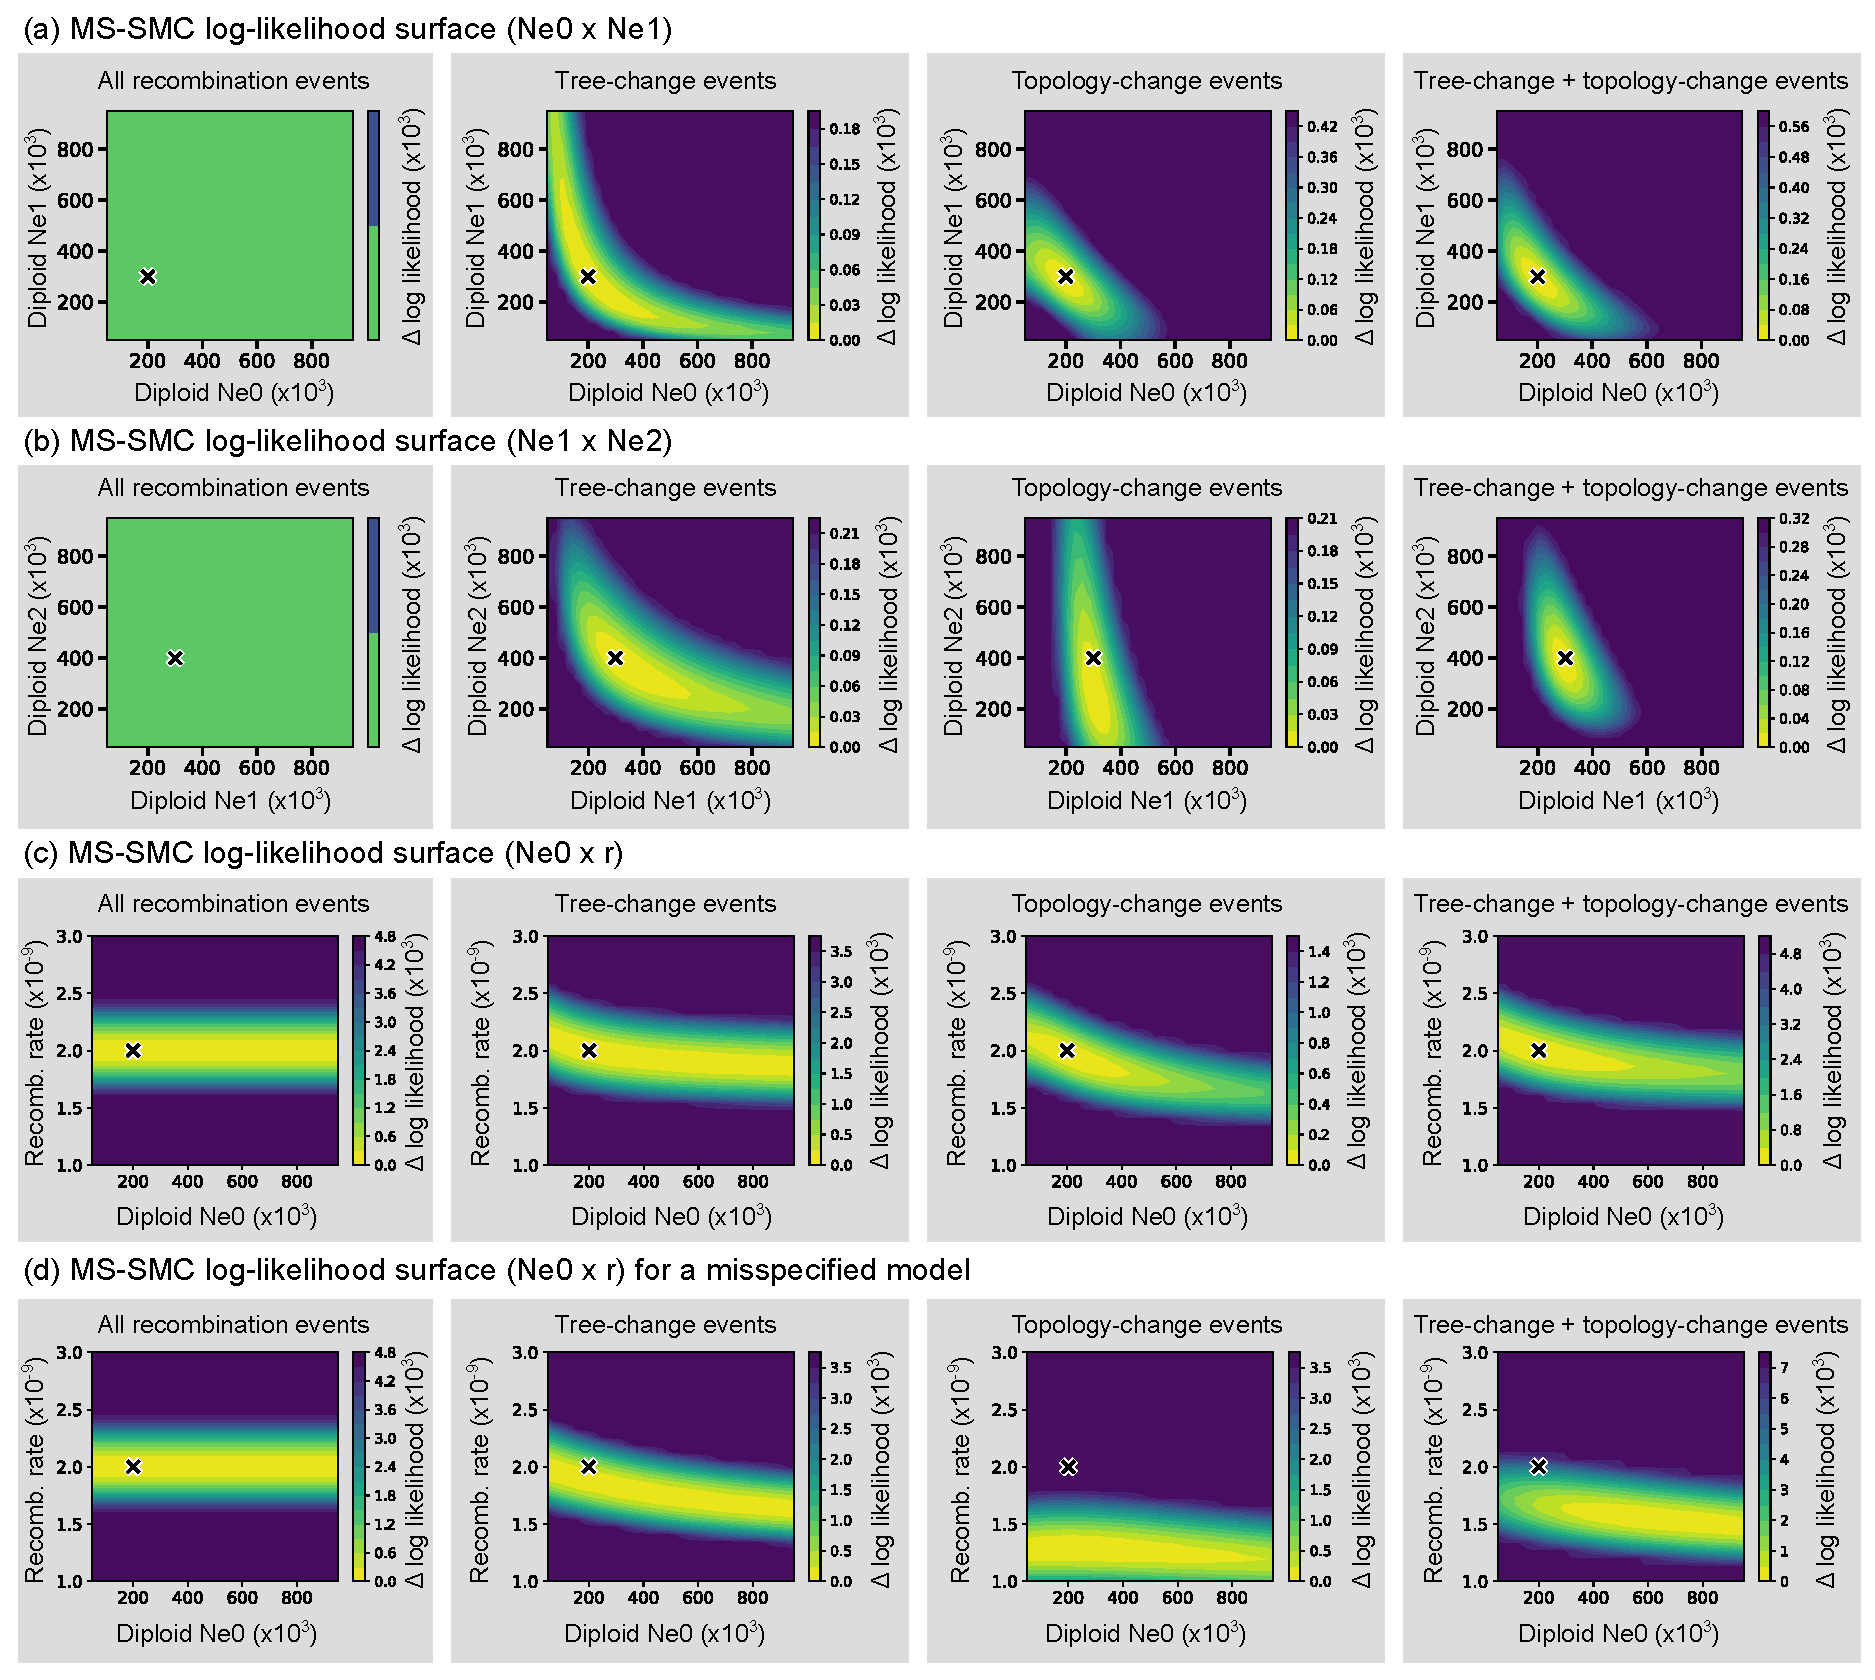
\includegraphics[width=0.95\textwidth]{figures/FigX-ARG-likelihood-2024-09-30
	\includegraphics[width=0.99\textwidth]{figures/current/Fig7-likelihood-surfaces-MCMC3.pdf}
	\caption{
		Implementation of a likelihood framework for fitting MSC model parameters
		to waiting distances in an ARG. Tree sequences were simulated under a 
		2-population demographic model with four MSC parameters ($N_e$0=200K, 
		$N_e$1=300K, $N_e$2=400K, $W$=1M) and recombination rate $r$=2 x 10$^{-9}$. 
		Log-likelihood surfaces are shown for two parameters at a time while fixing
		other parameters to their true value. True values are marked by an X.
		(a-c) Waiting distances between all recombination events provide no information
		for estimating MSC parameters, but the waiting distances between tree-change 
		and topology-change events are informative about MSC parameters, both
		individually and in combination.
		(d) When waiting distances derived from a 2-population model are used to 
		fit parameters in a single-population model they provide poor estimates
		of MSC parameters.
	}
	\label{fig:likelihood-surfaces}
\end{figure}


% simulation setup for likelihood surfaces and MSC optimization
\textcolor{red}{
We implemented this approach to evaluate MSC model parameters 
using waiting distances in an ARG simulated under a two-population MSC model with 
variable $N_e$ ($N_e$0=200K, $N_e$1=300K, and $N_e$2=400K), a divergence time
$W$=1M generations, and recombination rate $r$=2e-9. We sampled four 
genomes per population, and simulated 50 independent tree sequences 
each 400Kb in length (20Mb total) under the full coalescent with 
recombination model.
% 
This yielded 235,872 intervals between recombination events
(mean +/- S.D. length = 84.79 +/- 92.90), composing 
160,501 intervals between tree-change events
(mean +/- S.D. length = 124.56 +/- 135.68),
and 59,288 intervals between topology-change events
(mean +/- S.D. length = 336.93 +/- 441.72).
% 
To examine the information contained in different waiting distance data
sets we visualized 2D log-likelihood surfaces over a grid of 
values for pairs of MSC model parameters, while keeping all other 
parameters fixed at their true values.
}

\textcolor{red}{
We compared log-likelihood surfaces for four different sources of waiting
distance information, comprising the waiting distances between all 
recombination events, between only tree-change events, between only 
topology-change events, and for the combined log-likelihoods from both 
tree-change and topology-change waiting distances. 
(Fig.~\ref{fig:likelihood-calculation}e). 
% 
% Add paragraph here on combining.
Note that combining tree-change and topology-change likelihoods may seem 
like double-counting of information, since topology-change events are a
subset of the events that compose a tree-change event, in our terminology.
However, our equation for the probability of a topology-change event is 
conditional only on $\mathcal{S}$ and $\mathcal{G}$, and not on the probability 
of one or more tree-change events.
% 
In addition, it is clear conceptually that these two types of event 
probabilities have different relationships with a species tree.
% 
As an example, consider a genealogy that has two genomes sampled per species,
and is embedded in a species tree with very low $N_e$ such that ILS is nearly 
impossible. The probability of a topology-change event approaches zero
in this scenario, whereas the probability of a tree-change event is
much less affected by species tree barriers, since this event type can still 
occur within each species tree interval as a change in coalescent times.
% 
We demonstrate below how the likelihood of a demographic model can be more
robustly assessed by jointly incorporating both types of waiting distance
observations into the likelihood calculation.
% 
% Consequently, we can treat these two probabilities as independent, and 
% combine the likelihoods for each type of waiting distance observation.
}

% 
\textcolor{red}{
The log-likelihood surfaces show that waiting distance information
in an ARG is informative for estimating MSC model parameters when 
analyzed under our MS-SMC model framework
(Fig.~\ref{fig:likelihood-surfaces}). 
% 
The waiting distances between all recombination events, which do not take into
account the event type, provide no information for estimating MSC model 
parameters. By contrast, tree-change and topology-change waiting distances 
exhibit distinct ridges or peaks near the true parameter values
(Fig.~\ref{fig:likelihood-surfaces}a-c).
% significant information for estimating MSC model 
% parameters, with each surface exhibiting a peak that includes the true 
% simulation values...  This includes
A ridge in the likelihood surface suggests some uncertainty and potential
correlation structure. However, the rounder surface with more distinct peaks,
seen in the combined likelihood surface from both tree-change and 
topology-change waiting distances, exhibits less uncertainty and 
correlation, suggesting the combined information from multiple waiting distance
types provides the most accurate inference 
(Fig.~\ref{fig:likelihood-surfaces}a-c).
% The likelihood surfaces for joint Ne values sometimes exhibit a ridge
% when estimated from tree-change or topology-change distances, suggesting
% some uncertainty and a potential correlation structure. 
% However, their
% combined likelihood surface exhibits a more round shape with a peak 
% near the true values, suggesting less uncertainty and correlation.
We also used the same ARGs, simulated under a two-population
model with five parameters, to examine the likelihood surface under an incorrect 
demographic model, based on a single population model with two parameters.
(Fig.~\ref{fig:likelihood-surfaces}d). 
Here, the waiting distance data are a poor fit to the model, providing
inaccurate estimates of model parameters, especially from topology-change 
waiting distances. This suggests that topology-change waiting distances may be
particularly informative for model selection between demographic models, 
such as comparing species tree topologies.
}

% This yielded 40,720 tree-change events, with a mean length of 123 sites, 
% and 15,274 topology-change events, with a mean length of 325 sites. To visualize
% 2D likelihood surfaces, we computed the log-likelihood over a grid of 
% values for pairs of MSC model parameters, while keeping other parameters
% fixed at their true values.
% 

% The summed log-likelihoods from both tree 
% and topology change distances provided the most informative likelihood surface
% (Fig.~\ref{fig:fig-likelihood}d) \textcolor{red}{, which was consistent with our 
% expectation that the waiting distance distributions for tree and 
% topology changes together are more informative than either distribution on its own}.
% We also inferred a likelihood surface for a misspecified model, in which 
% the genealogies were generated under a 2-population model, but 
% the $\Lambda_g$ rate parameters were calculated for a single population 
% model with constant $N_e$. This model misspecification introduced a significant 
% bias in parameter estimation, shifting the likelihood surface towards lower $r$ 
% and higher $N_e$ (Fig.~\ref{fig:fig-likelihood}e). This demonstrates that even 
% for a simple two population model, ignoring population structure can significantly
% bias spatial genealogical inference methods.

% \textcolor{red}{
% \sout{
% The likelihood surface for tree-change distances exhibited a ridge containing 
% the true parameter values (Fig.~b), while the 
% topology-change likelihood surface exhibited a distinct peak at the true values
% (Fig.~c). 
% The summed log-likelihoods from both tree 
% and topology change distances provided the most informative likelihood surface
% (Fig.~d) 
% We also inferred a likelihood surface for a misspecified model, in which 
% the genealogies were generated under a 2-population model, but 
% the $\Lambda_g$ rate parameters were calculated for a single population 
% model with constant $N_e$. This model misspecification introduced a significant 
% bias in parameter estimation, shifting the likelihood surface towards lower $r$ 
% and higher $N_e$ (Fig.~\ref{fig:fig-likelihood}e). This demonstrates that even 
% for a simple two population model, ignoring population structure can significantly
% bias spatial genealogical inference methods.
% }
% }

\begin{figure}[tbp!]
	\centering
	%\fbox{\rule[-.5cm]{4cm}{4cm} \rule[-.5cm]{4cm}{0cm}}
	% 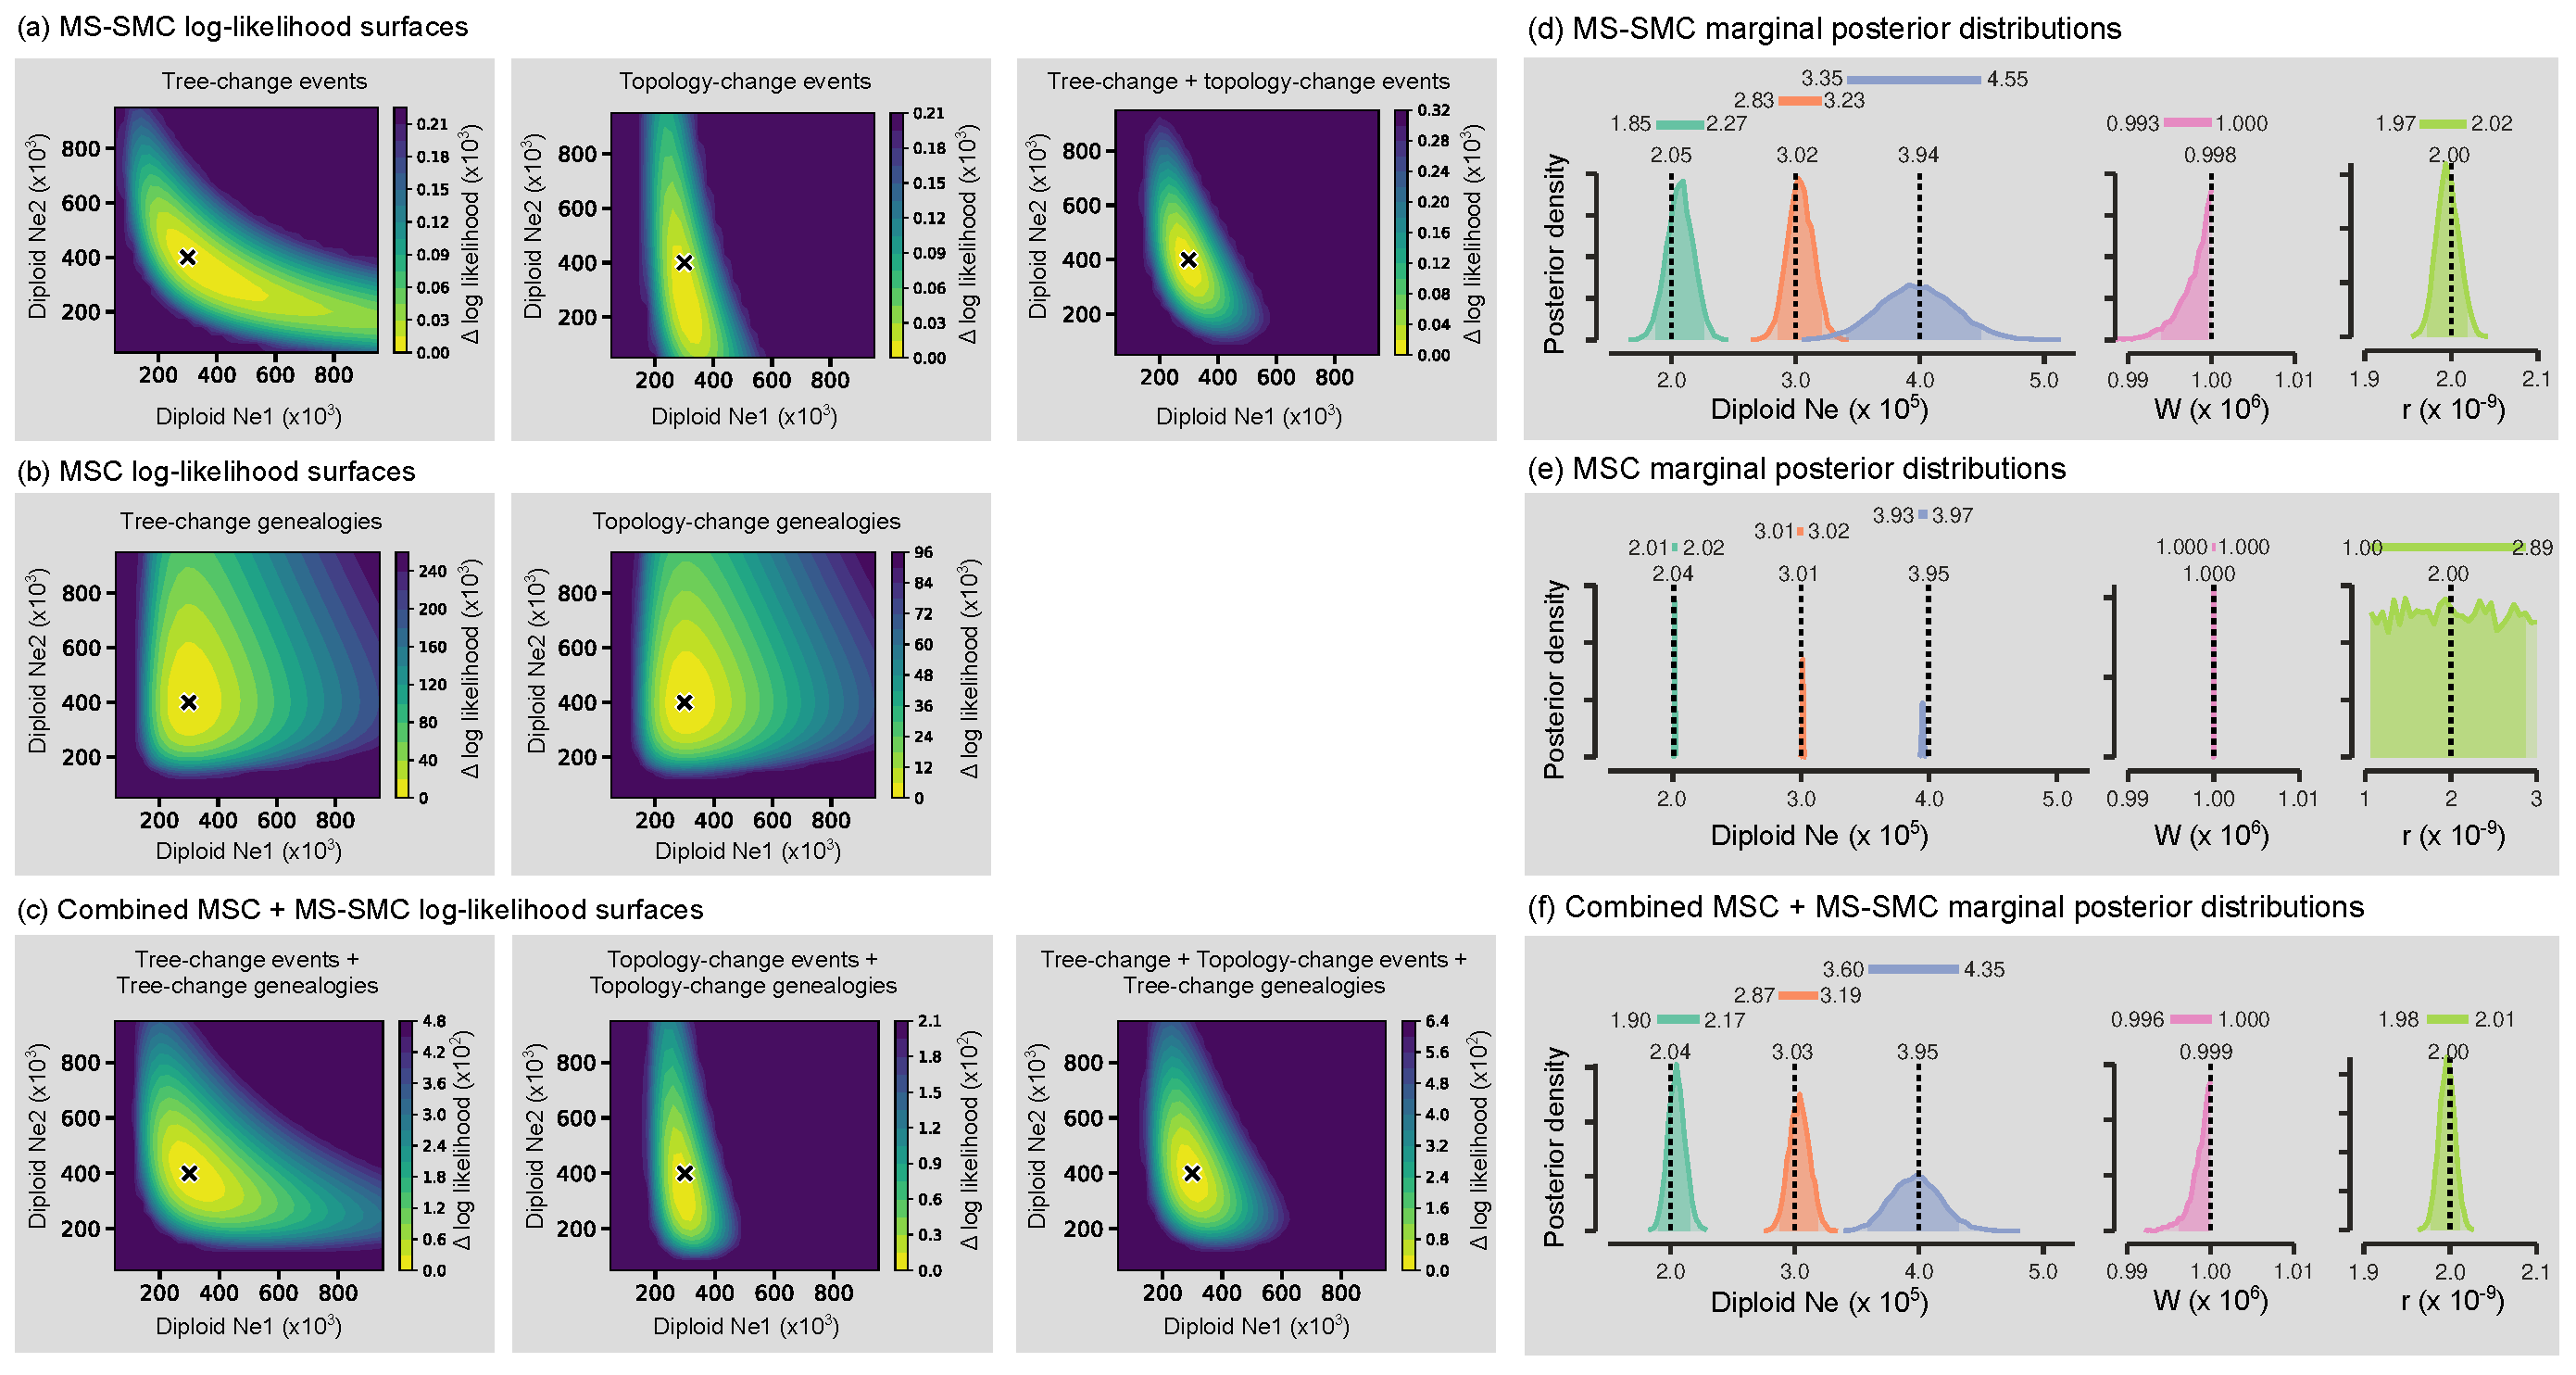
\includegraphics[angle=90, width=0.6\textwidth]{figures/current/Fig8-MSC-SMC-surface-and-posterior2.pdf}	
	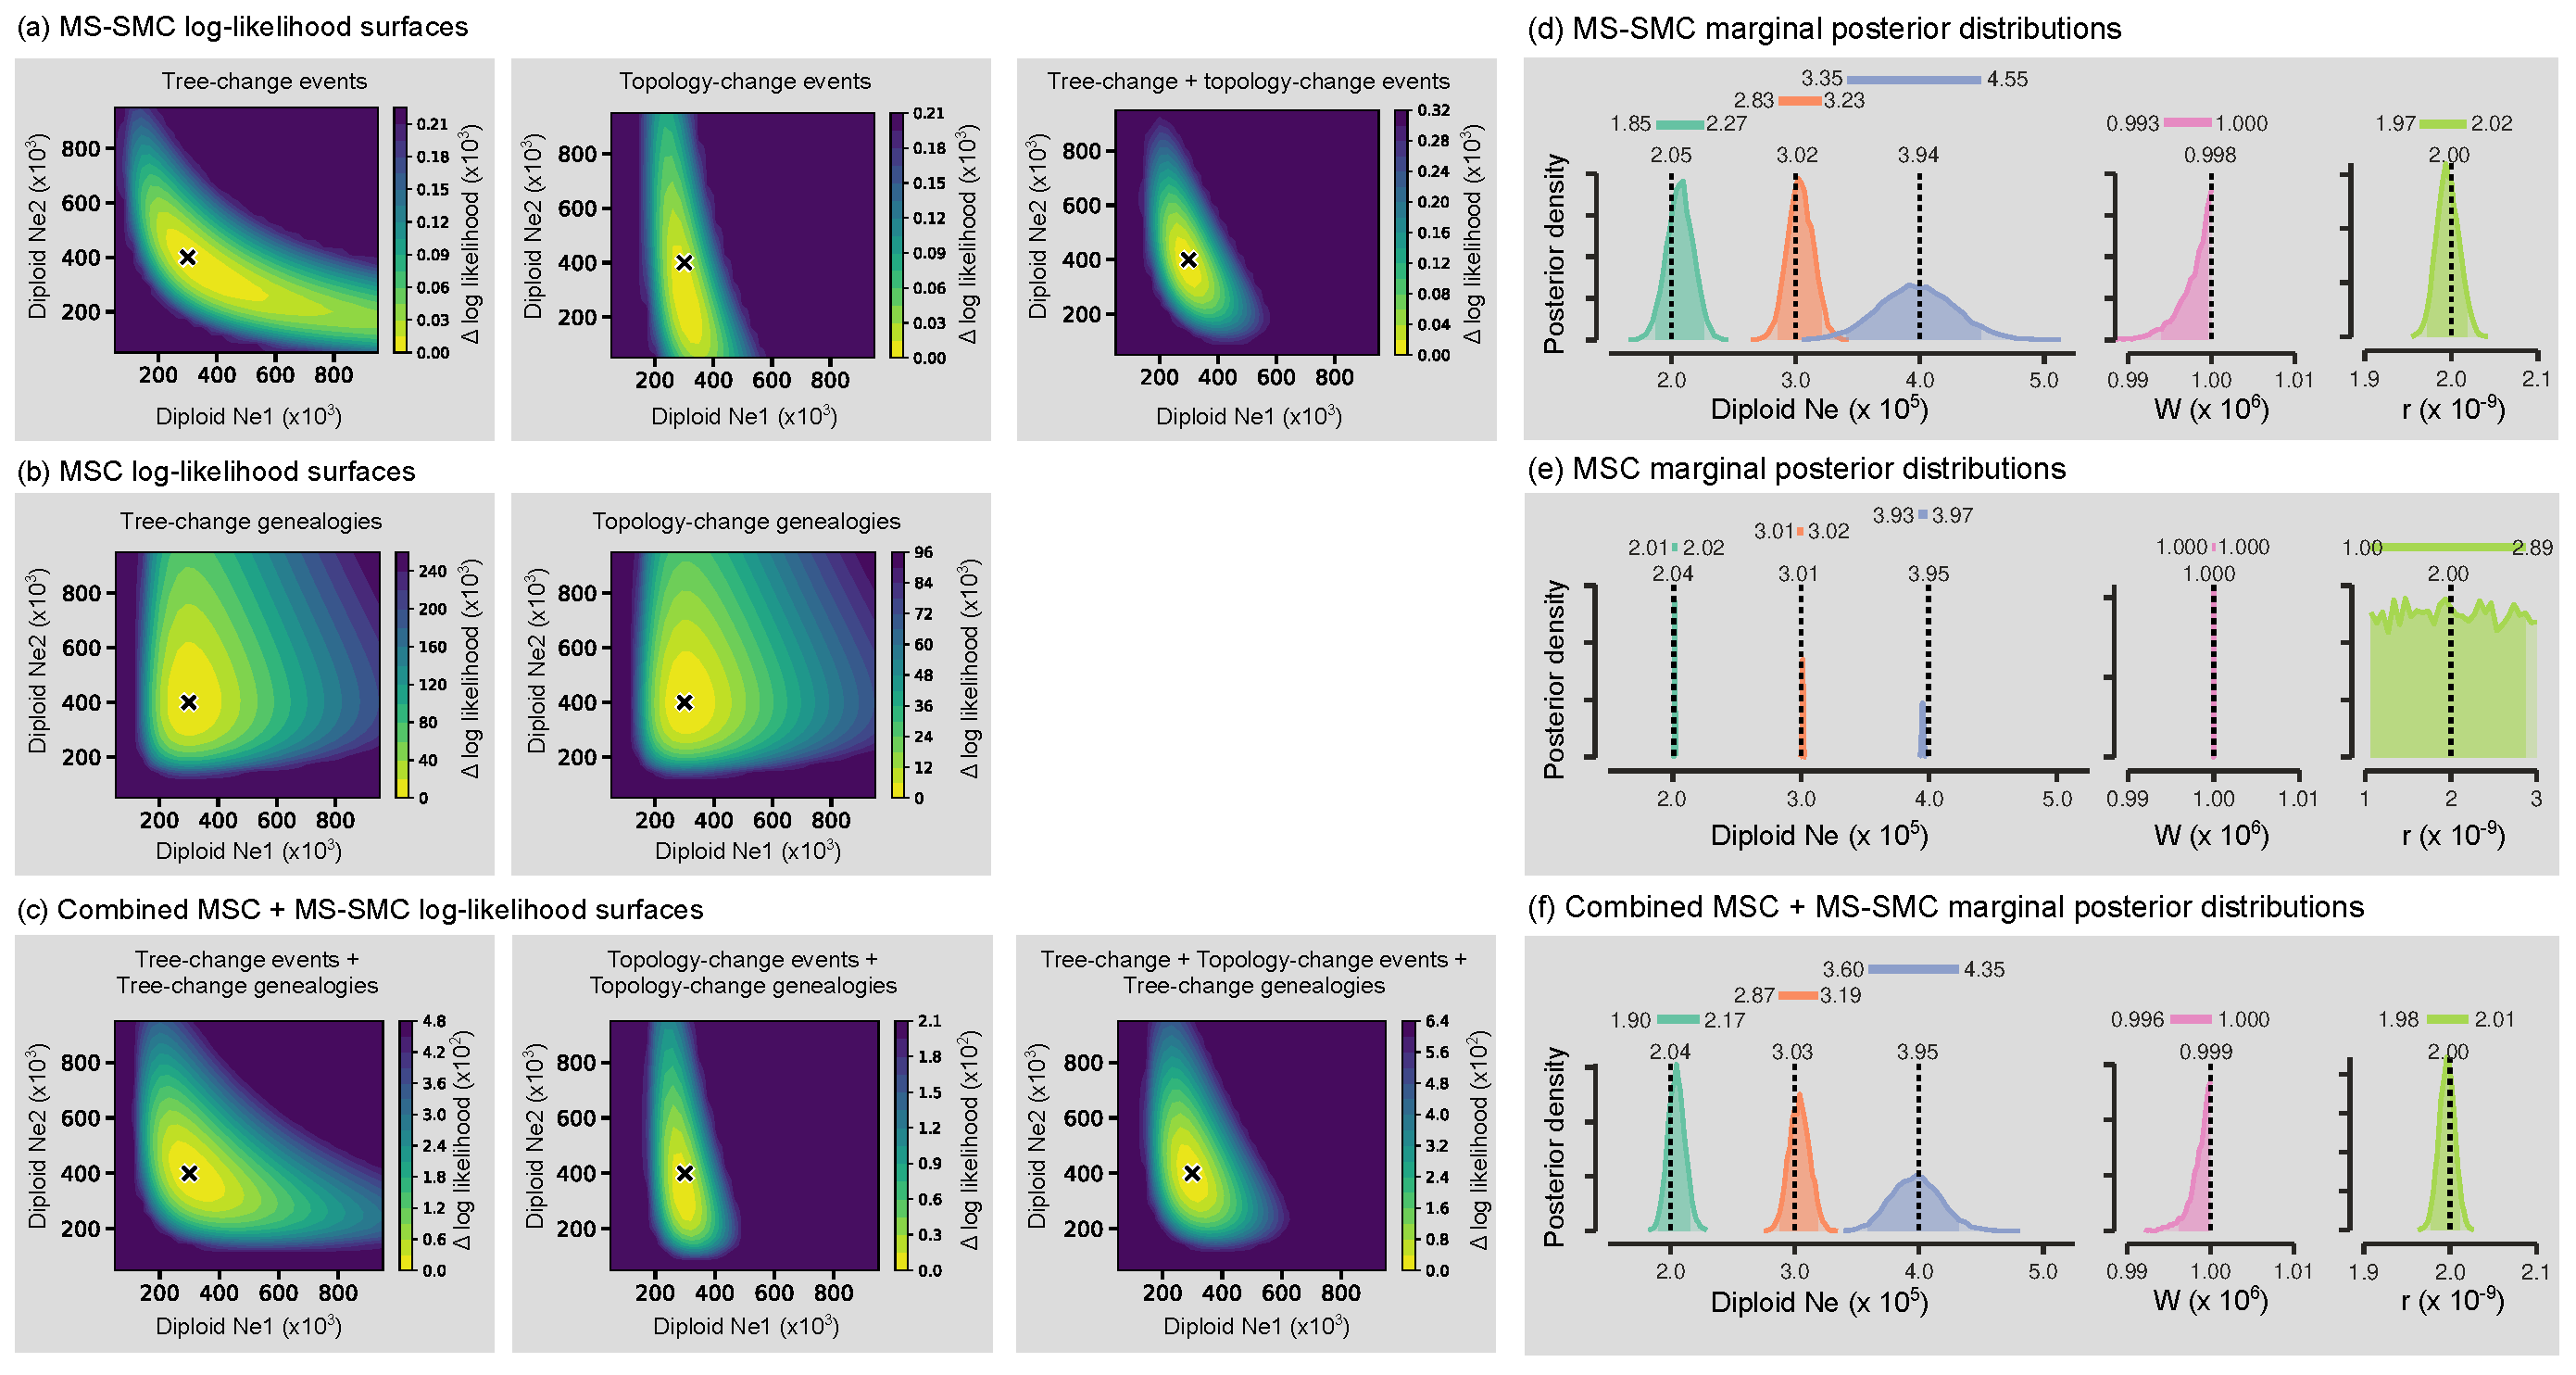
\includegraphics[width=0.99\textwidth]{figures/current/Fig8-MSC-SMC-surface-and-posterior2.pdf}		
	% 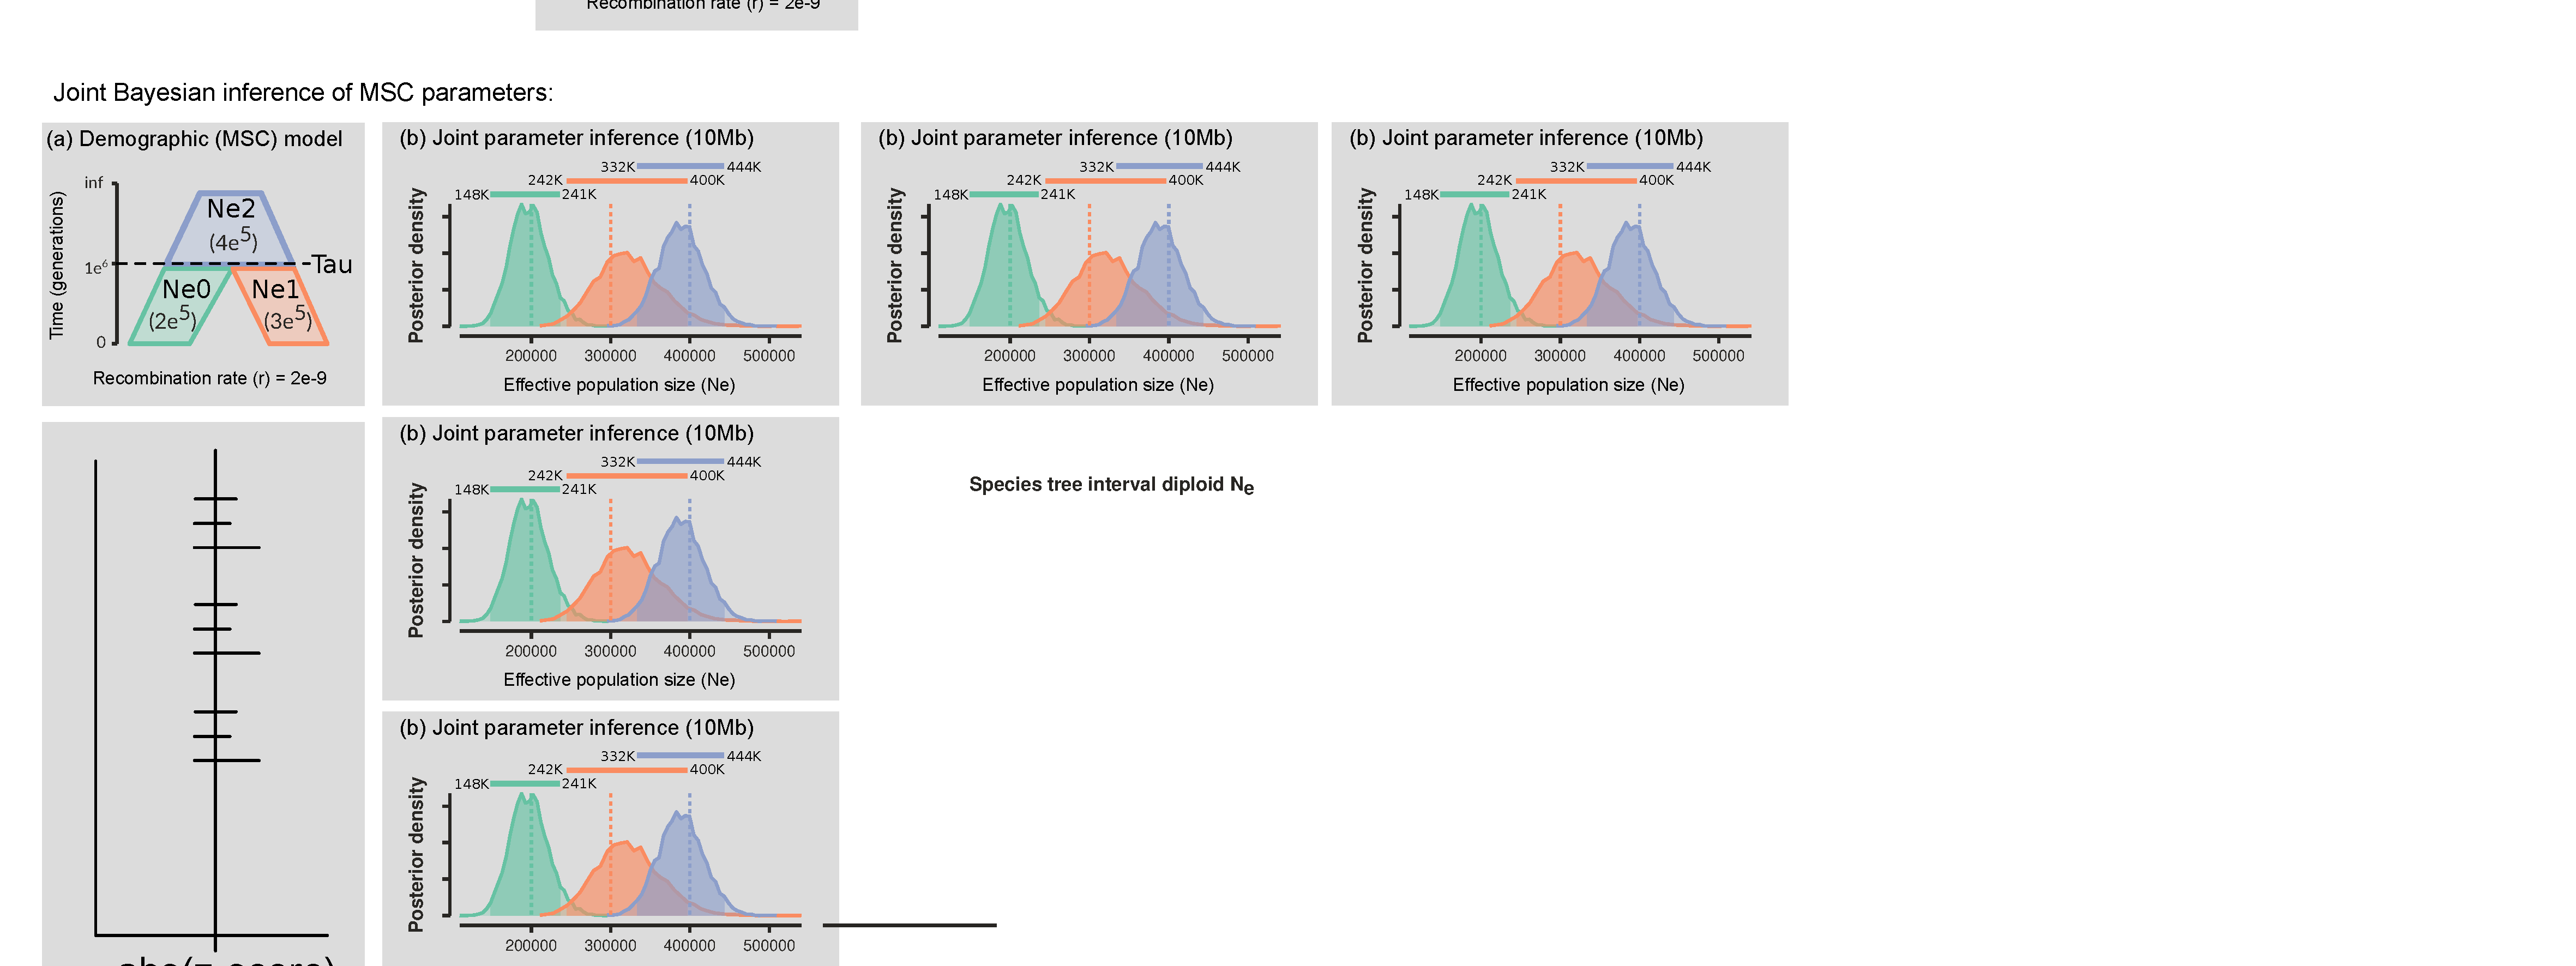
\includegraphics[width=0.95\textwidth]{figures/current/Fig8-likelihood-posteriors.pdf}
	\caption{
		\textcolor{red}{
		A comparison of likelihood-based model inference under the MS-SMC 
		versus MSC models -- i.e., when analyzing the waiting distances of
		genealogies versus the coalescent times in genealogies, respectively.
		% 
		% A comparison of the information contained in the likelihoods of genealogies
		% and the intervals lengths that they span in an ARG. 
		(a-c) Log-likelihood surfaces for parameters $N_e$1 and $N_e$2 based on 
		(a) waiting distance likelihoods computed under the MS-SMC;  
		(b) genealogy likelihoods computed under the MSC; or
		(c) the combined log-likelihoods of both types of data. 
		% 
		Note, MSC log-likelihoods are greater than MS-SMC log-likelihoods and 
		were down-weighted to a similar scale when combined.
		% 
		% In the latter case, the MSC log-likelihoods are multiplied by 0.001 to 
		% be on a similar scale as MS-SMC
		% from the sum of genealogy likelihoods
		% and one or more waiting distance likelihoods provide more accurate
		% and unbiased surfaces than from waiting distances alone. 
		(d-f) The marginal posterior distributions of demographic model parameters 
		$N_e$0, $N_e$1, $N_e$2, $W$, and $r$ jointly estimated using Bayesian inference.
		% 
		True demographic model parameters are indicated by a dashed black line, above 
		which the marginal posterior mean and 95\% HPD interval are shown.
		The marginal posterior distributions correspond to model parameter inference
		from (d) combined tree-change and topology-change waiting distances;
		(e) coalescent times of genealogies between tree-change events; and 
		(f) the combined likelihoods of the data used in the previous two analyses, 
		equally weighted.
		}
	}
	\label{fig:likelihood-posteriors}
\end{figure}
% \clearpage

Building on the high accuracy of our MS-SMC model, as suggested by the likelihood
surfaces, we proceeded to fit a full MSC model by jointly estimating all four MSC
model parameters and the recombination rate from waiting distance data.
We applied a Bayesian approach using the Metropolis-Hastings Markov chain Monte
Carlo (MCMC) algorithm to obtain the joint posterior probability distribution of
all parameters. For this, we set uninformative uniform priors on each parameter,
using U(1e5, 1e6) for $N_e$ parameters, U(1e5, 2e6) for $W$, and U(1e-9, 3e-9) for $r$.
Four separate MCMC chains were each initiated from different random seeds, and 
each run on the same simulated ARGs from above, using the
combined likelihood of both tree-change and topology-change waiting distances.
The first 500 iterations were excluded as burn-in and used to tune the proposal 
mechanism to achieve approximately 60\% acceptance rates. From each chain, we sampled
2,000 posterior values, sampling every 10 iterations. All parameters in each chain
were assessed for convergence to confirm that ESS scores exceeded 200. The four chains 
were then joined into a single combined posterior.

Our Bayesian implementation of the MS-SMC model shows that demographic model 
parameters can be accurately estimated from waiting distance information alone.
Using waiting distances simulated under a complex two-population model with 
variable $N_e$, we recovered accurate marginal posterior estimates for all three 
$N_e$ parameters, as well as the divergence time and recombination rate 
(Fig.~\ref{fig:likelihood-posteriors}d). 
Note that the marginal posterior for the divergence time ($W$) is truncated 
slightly above the true value, since values above this do not allow for
all genealogies to be embedded in the demographic model, and were thus
rejected. 
% 
This could be handled more appropriately by using more advanced priors on $W$. 
Across all parameters of the demographic model the true simulated values
fall within the inferred marginal 95\% highest posterior density (HPD) intervals.
% 
This demonstrates that the tree-change and topology-change waiting distances
in an ARG contain sufficient information when evaluated under the MS-SMC model
to jointly infer all parameters of a reasonably complex demographic model.



\subsection{Combining MS-SMC and MSC likelihoods}
Finally, we compared the information contained in the lengths of 
genealogy or topology intervals (i.e., waiting distances examined under the
MS-SMC) to the information contained in the trees within those intervals 
(i.e., coalescent waiting times examined under the MSC). 
% 
Using the same simulated ARGs from above, we computed the log-likelihood
of MSC model parameters by evaluating the probabilities of only the 
genealogies between tree-change or topology-change events under the MSC,
only the waiting distances of those genealogies under the MS-SMC, 
or using both log-likelihoods combined.
% 
For MSC calculations, the probability of each genealogy was weighted 
by the length of sequence that it spanned, as this greatly improved
accuracy compared to equal weighting, and provides the same precision 
of ARG information to the MSC model as is provided to the MS-SMC model.
% 
For MSC calculations we did not combine the probabilities of genealogies
that occur between both tree-change and topology-change events, as this
would represent double-counting of the same exact trees.


The log-likelihood surface of $N_e$ parameters computed under the MSC model
was less tightly concentrated near the true values than under the MS-SMC model,
but exhibited a more round shape, suggesting less uncertainty and minimal 
correlation between parameters 
(Fig.~\ref{fig:likelihood-posteriors}a-b).
The log-likelihood of the true parameter values under the MSC model
was approximately 12 times greater than under the MS-SMC model, 
reflecting that there is generally much more information in the coalescent 
times in a genealogy than in the interval length that it spans.
Similarly, the $\Delta$log-likelihood across the examined parameter space 
was much larger under the MSC model.
% 

When evaluating model parameters based on multiple criteria, inference can 
be improved if the corresponding likelihood surfaces exhibit orthogonal or 
complementary structures, as we observed here between the MSC and MS-SMC
likelihood surfaces. 
% 
Such differences in their shapes allow each criterion to provide unique 
information about the parameter space, which can improve the precision 
and robustness of optimization, as we showed previously for combining tree-
and topology-change waiting distances.
% To effectively combine
% the likelihood terms that are on different scales, prior distributions are 
% sometimes introduced to appropriately weight each term. 
Here, we implemented a simple weighting scheme, 
by uniformly dividing the MSC log-likelihoods by 1000, as this 
visually led to an intermediate shape of the likelihood surface.
% by uniformly dividing the MSC log-likelihoods by 12, so that the maximum 
% likelihood at the true parameter values would be similar under each model.
% 
The resulting combined likelihood surfaces (Fig.~\ref{fig:likelihood-posteriors}c)
are more narrowly concentrated around the true values than under the MSC
model alone, and generally exhibit rounder more peaked surfaces than under
the MS-SMC model alone. 


We next applied our Bayesian joint inference framework to estimate all five 
parameters using genealogy likelihoods, or combined genealogy and waiting 
distance likelihoods. 
As before, four separate MCMC chains were run on the same ARGs from different
starting seeds, checked for convergence criteria, and then combined.
% 
The marginal posterior distributions inferred from genealogy likelihoods 
were very narrow for all parameters except $r$, for which the MSC model
provides no information, and thus returned the prior
(Fig.~\ref{fig:likelihood-posteriors}e). 
% 
The true values did not fall within the 95\% HPD intervals for the $N_e$
parameters, despite the posterior means being very close to the true 
values. 
This may reflect a slight bias within our MCMC implementation, or be caused
by the non-independence of genealogies being analyzed under the MSC model.
% 
Despite this, we predicted that the combined information from genealogies
and waiting distances will provide a more accurate estimate of MSC 
parameters than from waiting distances alone, since the combined data 
tend to exhibit a more peaked and uncorrelated log-likelihood surface.
% 
As predicted, the marginal posterior distributions inferred from these data
are more narrow and accurate than from waiting distances alone
(Fig.~\ref{fig:likelihood-posteriors}f), with all true values falling 
within the inferred 95\% HPD intervals.
% 
This confirms that the information contained in tree- and topology-change
waiting distances is not redundant with the information contained in 
genealogy coalescent times, and that these observations can be combined
to provide additional information to evaluate the fit of an observed
or proposed ARG to a demographic model.
% Overall, this shows that the intersection of information contained 
% in genealogies and waiting distances, i.e., the information
% in an ARG, can be used to obtain accurate estimates of demographic
% model parameters.

% both the MSC to compute genealogy likelihoods and the MS-SMC to compute
% waiting distance likelihoods, can serve as an accurate statistical framework 
% for analyzing ARG data in the context of a parameterized structured 
% demographic model, such as a species tree.
% Overall, our analyses show that a combined likelihood framework using 
% both the MSC to compute genealogy likelihoods and the MS-SMC to compute
% waiting distance likelihoods, can serve as an accurate statistical framework 
% for analyzing ARG data in the context of a parameterized structured 
% demographic model, such as a species tree.

% When measuring the accuracy of each parameter
% as a z-score, representing the number of standard deviations of the posterior
% that the posterior mean deviates from the true values, the combined model
% exhibits the lowest error (Table~SX).
% 

% In answer to our more specific question of whether genealogy and waiting distance
% likelihoods can be combined to provide more accurate inference than from waiting
% distances alone, we 
% (Fig.~\ref{fig:likelihood-posteriors}f).
% The marginal posterior distributions inferred from the combined genealogy and
% waiting distance likelihoods provided the most accurate demographic model 
% parameter inference
% (Fig.~\ref{fig:likelihood-posteriors}f).
% 
% The range of the 50\% HPD for the ancestral population (Ne2) is larger than for the two
% extant populations, and has a mean that deviates farthest from the true value. This
% may be because fewer coalescent events occur in this interval, or because few 
% 
% We implemented a Bayesian inference using a Metropolis-Hastings Markov 
% chain Monte Carlo (MCMC) algorithm to compute a joint posterior 
% probability distribution of the five model parameters. 
% (Fig.~\ref{fig:fig-likelihood-posterior}a). 
% We set uniform priors on all ...three $N_e$ parameters between 
% 1e$^2$ and 1e$^7$, and ran a single MCMC chain to sample 10K 
% values, sampling every 5th iteration following a 1K iteration burnin. 
% For simplicity, we fixed the population divergence time and
% recombination rate to their correct values to focus solely on 
% $N_e$ estimation. 

% parameter inference under more complex MSC models we 
% implemented a Bayesian approach using a Metropolis-Hastings Markov 
% chain Monte Carlo (MCMC) algorithm to compute the joint posterior 
% probability distribution of multiple $N_e$ parameters for a 
% 2-population model with variable $N_e$ of 200K, 300K, or 400K
% (Fig.~\ref{fig:fig-likelihood-posterior}a).
% The input ARGs were simulated under this more complex MSC model but otherwise
% used the same settings as in the example above.
% % , and in this case, we sampled 8 haplotypes per population. 
% We set a uniform prior on all three $N_e$ parameters between 
% 1e$^2$ and 1e$^7$, and ran a single MCMC chain to sample 10K 
% values, sampling every 5th iteration following a 1K iteration burnin. 
% For simplicity, we fixed the population divergence time and
% recombination rate to their correct values to focus solely on 
% $N_e$ estimation. 

% 
% 
% It would be better to describe this as falling within a X% 
% credible interval.
% 

% This paves
% the way for a new mode of phylogenetic inference, where 
% a road for future 
% paving the way for new phylogenetic inference methods 
% that can analyze linked genome data for species tree inference.
% Further theoretical and empirical work will be needed to
% explore this in greater detail.

%  in that it confirms that 
% considering that it may be possible, under
% some MSC models, for many different parameter combinations to yield 
% similar waiting distance expectations, which could cause identifiability
% issues. However, by combining information from both tree and topology 
% waiting distances this problem may be reduced. Our results suggest 
% that MSC model parameters can be identifiable from genealogical 
% waiting distances, at least for relatively simple models like the ones
% examined here, 

% =======
% The input ARGs were simulated using the same settings as above, 
% %but under this more complex MSC model, and in this case, 
% %we sampled 8 haplotypes per population. We set a uniform prior on 
% except that we used this more complex MSC model and
% sampled 8 haplotypes per population. We set a uniform prior on 
% $N_e$ between 1e$^2$-1e$^7$ and ran the MCMC chain to sample 
% 10K values, sampling every 5th iteration after a 1K iteration 
% burnin. For simplicity, we fixed the population divergence time to 
% the correct value of 500K and focused solely on $N_e$ estimation. 

% The resulting maximum \emph{a posteriori} probability estimates of 
% model parameters are highly accurate, all falling within 0.5 
% standard deviations of the true values 
% (Fig.~\ref{fig:fig-likelihood-posterior}b). 
% This result is encouraging, considering that it may be possible under
% some MSC models for many different parameter combinations to yield 
% similar waiting distance expectations, potentially causing identifiability
% %issues. However, by combining information from both tree and topology 
% %waiting distances this problem may be reduced. Our results suggest 
% issues. However, combining information from both tree and topology 
% waiting distances may help address this problem. Our results suggest 
% that MSC model parameters will sometimes be identifiable from genealogical 
% waiting distances, at least for relatively simple models like the ones
% examined here. Further theoretical and empirical work will be needed
% to explore this question in greater detail.
% >>>>>>> 8a0665285dacae9af3b3045ce3fbb7b870619d5a
% Anecdotally, we found that using multiple independent ARGs improves 
% the accuracy of this joint inference method compared to a single 
% larger ARG. This suggests that ...


% MSC model parameters can predict waiting distances, we can also perform the 
% inverse operation, and find the maximum likelihood MSC model to explain a
% set of observed 

% Given a proposed or observed ARG, can we use MSC model parameters to find 
% ...

% Finally, we demonstrated that a known sequence of genealogies paired 
% with the accompanying observed waiting distances to next topological change 
% for each can be used to estimate the Ne value for species trees with different
% topologies (Fig.~\ref{fig:fig4}). We used two different species trees: one 
% imbalanced, 5-tip tree with internode branches of equal length, and one 10-tip tree
% with an irregular topology and branches of variable lengths. Both species 
% trees were assigned equal root heights of 1e6 generations and equal Ne values of 150000 on all 
% branches, and we simulated a 5e6-bp chromosome for each using \emph{ipcoal}. We broke each 
% chromosome down into its component "initial genealogies" -- those that start each segment 
% bounded by changes in topology -- and the accompanying segment lengths (i.e. waiting 
% distances). Using these values and a known recombination rate of 1e-9 recombs/bp/generation, 
% we calculated the likelihood that each of 41 proposed Ne values produced the set of 
% genealogies and waiting distances. Using this approach, we recovered a correctly inferred Ne 
% value of 150000 for both trees.


% with larger Ne values. This occurs for two reasons: first, genealogies with longer 
% branches have a higher probability of any recombination event occurring, since the
% rate is proportional to the sum of edge lengths; second, when Ne is large it is 
% more likely that many genealogy edges will exist in the same species tree intervals
% together, 
% coalescent events are more likely to occur deeper in time


% brief methods description
% Next, we tested the effect of variation in basic species tree parameters on expected waiting 
% distances to tree changes and topology changes (Fig.~\ref{fig:fig3}). We started with four 
% different species trees: two imbalanced and two balanced. For each pair, we used a large tree 
% (10 tips), and a small tree (5 tips) that was pruned from the large tree, with internode 
% distances kept the same. On each species tree, we generated 1000 random \emph{unlinked} 
% genealogies using MSC probabilities and using 
% each of 9 evenly spaced Ne values, ranging from 50000 to 250000. We calculated the expected 
% waiting distance 
% to a tree change and to a topology change for each genealogy/species tree pair, assuming a 
% recombination rate of 1e-9 recombs/bp/generation. In Fig.~\ref{fig:fig3}, we show the mean 
% expected waiting distances to tree and topology changes for each species tree and for each Ne 
% value. The decline in expected waiting distances across Ne values and from small to large 
% trees demonstrates that, on average, waiting distances to tree and topology changes decrease 
% with increasing numbers of tips sampled and with increasing Ne values. 





% \begin{figure}[t]
% 	\centering
% 	%\fbox{\rule[-.5cm]{4cm}{4cm} \rule[-.5cm]{4cm}{0cm}}
% 	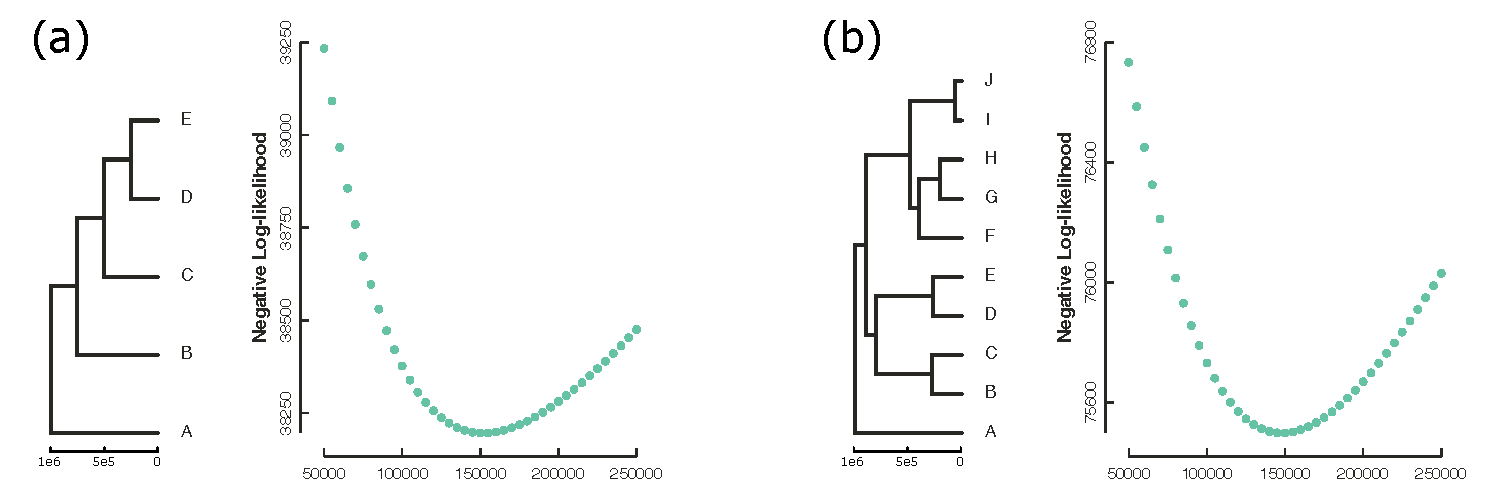
\includegraphics[width=0.9\textwidth]{figures/Fig6-constant_ne_inf.pdf}
% 	\caption{
% 		Inference of species tree Ne values from genealogies, observed waiting 
% 		distances to topology changes, and recombination rate. We generated two different 
% 		species trees: Both have root heights of 1e6 generations, but one has five tips, 
% 		an unbalanced topology, and identical internode lengths, while the other has ten 
% 		tips, an irregular topology, and irregular branch lengths. Using a recombination 
% 		rate of 1e-9 recombs/bp/generation and a constant Ne value of 150000 over all 
% 		branches, we generated a 5MB tree sequence from each species tree using 
% 		\emph{ipcoal}. Then, we decomposed the alignment into segments bounded by 
% 		topology changes in the genealogies, and we recorded the initial genealogy 
% 		for each segment. Finally, we calculated the likelihood of the set of 
% 		genealogies and waiting distances, along with the recombination rate, at 41 
% 		different proposed Ne values. For both sequence alignments, 150000 was 
% 		correctly inferred as the Ne value.
% 	}
% 	\label{fig:fig5}
% \end{figure}



% \begin{figure}[t]
% 	\centering
% 	%\fbox{\rule[-.5cm]{4cm}{4cm} \rule[-.5cm]{4cm}{0cm}}
% 	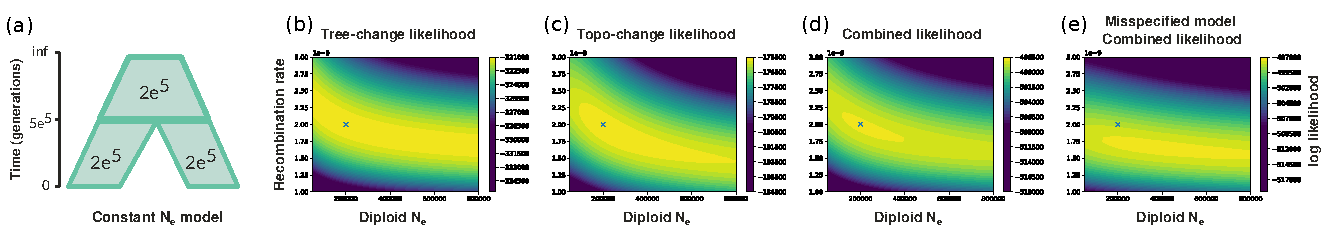
\includegraphics[width=0.99\textwidth]{figures/likelihood-figure3.pdf}
% 	\caption{
% 		MS-SMC likelihood framework. (a) ARGs were simulated under a
% 		two-population species tree model with a constant $N_e$=200K and 
% 		$r$=2e-9. (b) A joint log-likelihood surface for $N_e$ and 
% 		$r$ inferred from the distances between tree-change events; 
% 		(c) topology-change events; or (d) both. The true parameters are
% 		marked by an X. (e) If the MSC model is
% 		misspecified as a single-population model but the data derive from 
% 		a two-population model, likelihood inference	is highly biased.
% 		% ARGs were 
% 		% simulated under a two-population species tree model with variable 
% 		% $N_e$. (e) A joint posterior distribution of $N_e$ parameters inferred 
% 		% by Bayesian MCMC from tree and topology-change waiting distances.
% 	}
% 	\label{fig:fig-likelihood}
% \end{figure}

% \subsection{\textcolor{red}{Likelihood of an ARG Given a Species Tree}}
% \textcolor{red}{
% % Here we demonstrate an application of the MS-SMC theory to provide a new 
% % ...
% Using the ARG inference framework implemented in ARGweaver as an example, 
% an ARG can be estimated as a posterior sample of trees and interval lengths
% across a chromosome inferred through an MCMC sampling approach wherein the
% space of possible ARGs is explored conditional on the relative probability.
% For example, given a sequence alignment, and priors on recombination rate,
% effective populations size(s), and population structure, an SMC' algorithm 
% can be implemented to sample changes to trees, topologies, and/or interval
% break points. A new proposed ARG is either kept or discarded based on its
% likelihood relative to the current sampled ARG. In this approach, the MS-SMC
% can represent an improvement if its ARG likelihood measurement provides more
% information than the standard ARG likelihood measurement. To demonstrate that
% this is the case, we simulated a sequence alignment under our demographic
% model (ref) and sampled a posterior sample of 10K ARGs in ARGweaver. We then
% computed the likelihood of each ARG as the sum of the likelihood of the genealogies
% and interval lengths. Genealogy likelihoods were computed under the MSC, but
% with each genealogy likelihood divided by the proportion of length of the 
% chromosome that it represents. The likelihood of interval lengths was calculated
% from an exponential probability density. 
% % More intervals --> more events --> higher likelihood. That's bad.
% % ...
% Re-implementing the ARG sampling approach of ARGWeaver to perform MS-SMC 
% likelihood calculations during the MCMC sampling process is beyond the scope
% of this study.
% }

% and more informative framework for calculating the likelihood of an ARG.
% In contrast to the current approach which models the waiting distance
% between recombination events regardless of their event type 
% \citep[e.g.,][]{wiuf_ancestry_1999, kuhner_maximum_2000}, and without the ability 
% ... Fig.~\ref{fig:figS-bias-smc}
% our approach extracts more information from the spatial distribution of 
% genealogies by incorporating the probabilities of observing several different
% categorical types of recombination events, which span over varying and greater 
% distances. 
% ...
% provides a novel framework for
% calculating the likelihood of an ARG by combining spatial information extracted
% from multiple recombination events spanning varying distances of a
% chromosome.

% Because the 



%%%%%%%%%%%%%%%%%%%%%%%%%%%%%%%%%%%%%%%%%%%%%%%%%%%%%%%%%%%%%%%%%%%%%%%%%%%
%%%%%%%%%%%%%%%%%%%%%%%%%%%%%%%%%%%%%%%%%%%%%%%%%%%%%%%%%%%%%%%%%%%%%%%%%%%
%%%%%%%%%%%%%%%%%%%%%%%%%%%%%%%%%%%%%%%%%%%%%%%%%%%%%%%%%%%%%%%%%%%%%%%%%%%
%%%%%%%%%%%%%%%%%%%%%%%%%%%%%%%%%%%%%%%%%%%%%%%%%%%%%%%%%%%%%%%%%%%%%%%%%%%
%%%%%%%%%%%%%%%%%%%%%%%%%%%%%%%%%%%%%%%%%%%%%%%%%%%%%%%%%%%%%%%%%%%%%%%%%%%
%%%%%%%%%%%%%%%%%%%%%%%%%%%%%%%%%%%%%%%%%%%%%%%%%%%%%%%%%%%%%%%%%%%%%%%%%%%
%%%%%%%%%%%%%%%%%%%%%%%%%%%%%%%%%%%%%%%%%%%%%%%%%%%%%%%%%%%%%%%%%%%%%%%%%%%
%%%%%%%%%%%%%%%%%%%%%%%%%%%%%%%%%%%%%%%%%%%%%%%%%%%%%%%%%%%%%%%%%%%%%%%%%%%
%%%%%%%%%%%%%%%%%%%%%%%%%%%%%%%%%%%%%%%%%%%%%%%%%%%%%%%%%%%%%%%%%%%%%%%%%%%
%%%%%%%%%%%%%%%%%%%%%%%%%%%%%%%%%%%%%%%%%%%%%%%%%%%%%%%%%%%%%%%%%%%%%%%%%%%
%%%%%%%%%%%%%%%%%%%%%%%%%%%%%%%%%%%%%%%%%%%%%%%%%%%%%%%%%%%%%%%%%%%%%%%%%%%
%%%%%%%%%%%%%%%%%%%%%%%%%%%%%%%%%%%%%%%%%%%%%%%%%%%%%%%%%%%%%%%%%%%%%%%%%%%
%%%%%%%%%%%%%%%%%%%%%%%%%%%%%%%%%%%%%%%%%%%%%%%%%%%%%%%%%%%%%%%%%%%%%%%%%%%
%%%%%%%%%%%%%%%%%%%%%%%%%%%%%%%%%%%%%%%%%%%%%%%%%%%%%%%%%%%%%%%%%%%%%%%%%%%


\section{Discussion}

% Restate the problem
Genealogical relationships vary spatially across chromosomes, reflecting 
a history of recombination between genome segments inherited from 
different ancestors. Such variation can be modeled by the sequentially 
Markov coalescent, which provides a generative process upon which 
many statistical methods have been developed \citep{mcvean2005approximating, spence_inference_2018}.
% 
However, most applications of the SMC' remain highly limited with regard to 
the scale over which they extract information from genomes -- extending forward 
just one recombination event at a time. 
By contrast, the recent development 
% \textcolor{red}{by \citet{deng_distribution_2021}}
by \citet{deng_distribution_2021}
of solutions for predicting 
tree- and topology-change waiting distances under the SMC' 
% \textcolor{red}{\sout{\citep{deng_distribution_2021}}}
effectively adds two additional, longer-range sources of information for 
any position in a genome. 
% \hl{In this original formulation,} 
In their model,
these distances are a 
result of the probabilities of different phenomenological outcomes of the 
SMC' process given a genealogy embedded in a single population coalescent
model with constant $N_e$.
% ^prob worth cleaning up this sentence
% within the constraints of a demographic model.
%regardless of the outcome for the genealogy \citep{terhorst_etal}. 
%However, 
%for many datasets, 
%this limits the information that is available for SMC-based inference methods, 
%recombination events between pairs of individuals will often be uninformative 
%and the signal in the sequence data resulting from changes in the underlying genealogies
%will be spread across larger distances and will simultaneously impact relationships among all samples. 
% In contrast, the recent solutions by \citep{deng_distribution_2021} for the probabilities 
% of different categorical types of recombination events (tree-changes and 
% topology-changes) focus on "thinning" out invisible recombination events -- 
% instead modeling impactful recombination events 
% that extend over great spatial genomic distances and affect the relationships among samples. 
% Further, these solutions are for the full genealogy of all samples simultaneously rather 
% than isolating a subset of samples and coalescences. 
Here we extended this framework, deriving new solutions for the probabilities 
of tree-change and topology-change events for a genealogy embedded 
in any arbitrarily parameterized
\textcolor{red}{species tree \sout{coalescent}} model. 
% 
\textcolor{red}{
While some previous studies have explored the impact of species tree parameters
on linked genealogical variation, their results have been limited to few specific
cases \citep[e.g.,][]{slatkin2006concordance}.
\sout{These solutions} 
Our generalized solutions here
}
lay a groundwork for 
\textcolor{red}{\sout{exploring} modeling}
how variation in species tree parameters 
affects neutral expectations of genealogical heterogeneity across chromosomes.

% \textcolor{red}{
% While previous work has explored patterns of linkage between
% two loci in a species tree 
% context and found similar influence of $N_e$ and species divergence times,
% such attempts have been limited to special cases \citep[e.g.,][]{slatkin2006concordance}.
% }
% \sout{These solutions} \textcolor{red}{Our generalized solutions here} 


% These solutions, extended from initial work by \citep{deng_distribution_2021}, 
% lay a groundwork for exploring how variation in species tree parameters 
% affects neutral expectations of genealogical heterogeneity across chromosomes.

% This provides a new framework for modeling spatial genealogical variation

% Summarize what we did
% We solved for the expected turnover rate in genealogical trees and topologies 
% along a genome under an arbitrary species tree topology with arbitrary 
% divergence times, and with arbitrary Ne values for each species tree branch.
%structuring the equations to accept an arbitrary species tree topology 
%and a different, arbitrary Ne value for each species tree branch. 
% These solutions, extended from initial work by \citep{deng_distribution_2021}, 
% lay a groundwork for exploring how variation in species tree parameters 
% affects neutral expectations of genealogical heterogeneity across chromosomes.


% Our primary result is the ability to predict length of a genealogy
\textcolor{red}{
The multi-species sequentially Markov coalescent (MS-SMC) is
\sout{Our MS-SMC approach provides}
}
a predictive model for the relationship between a parameterized species
tree and the length of a genomic interval over which a genealogy will 
\textcolor{red}{
span.
\sout{is expected to be observed}
}
% 
Within \textcolor{red}{\sout{our} this}
framework, demographic model parameters determine probabilities of coalescence
in species tree intervals and prevent coalescence between lineages that
are separated by species divergence events. 
\textcolor{red}{
This constrains the outcomes of the SMC' process, 
and thus the similarity of genealogies in sequential genomic intervals.
% separated by a recombination event. %in sequential intervals. 
By categorizing the continuous outcomes of this constrained SMC' process into 
few discrete categorical outcomes, we are able to compute the probabilities of 
each type, corresponding to recombination events that cause no change to the
genealogy, a tree-change, or a topology-change.
% 
\sout{
We demonstrated the accuracy of our implementation relative to stochastic 
simulations performed under both the full coalescent with recombination 
and the SMC' approximation 
}
% 
Using these solutions, the effect of MSC model parameters on the probability
of genealogical turnover can be computed and visualized for a single genealogy
(Fig.~\ref{fig:edge-probabilities}; Fig.~\ref{fig:figS-edge-probabilities}),
or for a distribution of genealogies simulated under an MSC model
(Fig.~\ref{fig:fig-validation}).
\sout{
The effects of MSC model parameters on spatial genealogical variation can 
be statistically modeled and visualized 
% (Fig.~\ref{fig:edge-probabilities}; Fig.~\ref{fig:figS-edge-probabilities}).
}
Using the latter approach, we demonstrated the accuracy of our solutions by
showing that the mean and variance of waiting distances predicted by our model
match closely to the results of stochastic coalescent simulations performed
on the same demographic model under the SMC' or full coalescent with 
recombination.
% citep{hudson1983properties,wiuf_recombination_1999,mcvean2005approximating}. 
\sout{
and our examples show that the neutral rate of turnover in genealogical trees
and topologies across a genome is highly dependent on species tree model parameters.
}
}
% feels like disconnected sentences

% Previously, lengths could only be simulated .But analytical methods are better.
A complex relationship exists between a parameterized MSC model, 
the distribution of genealogies that can arise under that model, and the 
spatial distances over which those genealogies are expected to span.
Previously, such patterns could only be examined through stochastic simulations. 
For example, \cite{mckenzie_multispecies_2020} used exhaustive simulations to
examine the effect of species tree parameters on 
\textcolor{red}{
the spanning length of genealogical topologies
\sout{genetic linkage}
}
by varying species tree length, size, and shape. 
% 
While this approach is practical for estimating the \emph{mean} linkage across
a large set of sampled genealogies under a specific demographic model, it is
impractical for estimating the persistence of \emph{individual} genealogies. 
% Indeed, a large distribution of simulated waiting distances would need to be 
% generated for every genealogy to obtain expectations.
% Simulation approaches are particularly intractable for studying sequences of 
% many genealogies, for which individual distributions would need to be
% generated for every tree in a sequence. 
% Similarly, it did not... more here please.
%\hl{In addition to providing fast calculations of waiting distances, 
%analytical solutions also offer the opportunity to develop likelihood-based
The analytical solutions presented here not only enable 
% Its not 'faster' than simulating data and just measuring the mean,std of 
% the simulated intervals. Since our mean,std calculation also requires 
% examining the distribution of simulated trees. 
\textcolor{red}{
calculating and comparing the expected interval lengths that different 
genealogies will span given their embedding in the same species tree, 
but also enabled the development of a statistical framework for computing 
the probability of an observed waiting distance spanned by a genealogy 
as a function of the species tree model.
}

% FINAL MAIN DISCUSSION PARAGRAPH ABOUT LIKELIHOODS
\textcolor{red}{
The multi-species coalescent is the foundation of modern phylogenetic 
methods that aim to infer a species tree as a hierarchical model within
which genealogical variation can be embedded
\citep{maddison1997gene,degnan2009gene,maddison2006inferring}.
% 
The parameters of this model can be estimated from the distribution
of coalescent times in genealogies, and many methods have been developed
on this framework including full likelihood based analyses of molecular
sequence data \citep{rannala2003bayes}, and pseudo-likelihood or summary
based methods that analyze inferred gene tree distributions
\citep{mirarab_multispecies_2021}. 
% The process of integrating over genealogical variation in multi-locus
% genomic datasets has become a foundation of modern methods in evolutionary
% genomics. 
% 
% The multi-species coalescent model played a significant role in this
% development, providing a framework for fitting parameters of a 
% species tree model based on the distribution of coalescent
% times among a set of embedded genealogies (or sequences modeled as 
% evolving on those genealogies)
% \citep{maddison1997gene,maddison2006inferring,rannala2003bayes}. 
% 
Here, we demonstrated that the parameters of a species tree model can 
alternatively be estimated from a completely new source of information,
in the form of the waiting distances between recombination events causing
a tree-change or topology-change between sequential genealogies in an ARG
(Fig.~\ref{fig:likelihood-posteriors}d).
% 
Examination of joint likelihood surfaces revealed that these two 
types of waiting distance observations provide non-redundant 
information that is complementary and orthogonal, such that when
combined they can intersect to provide more accurate estimates of 
model parameters
(Fig.~\ref{fig:likelihood-surfaces}a-b). 
% 
Similarly, although the information contained in tree- and topology-change
waiting distances is less than that contained in the coalescent times of the
same genealogies, we showed that these two sources of data can be combined,
and are also complementary and non-redundant
(Fig.~\ref{fig:likelihood-posteriors}c,f).
% 
We envision many future applications can build upon this joint framework for
evaluating the fit of ARGs to a demographic model using not only the
probabilities of genealogies within the ARG, but also the probabilities of
the spanning distances of topological features of those genealogies.
% between tree- and topology-change events.
Below we describe several of these envisioned applications.
%
% We envision many future applications can build upon this framework
% to improve methods for both species tree and ARG inference.
}

%%%%%%%%%%%%%%%%%%%%%%%%%%%%%%%%%%%%%%%%%%%%%%%%%%%%%%%%%%%%%%%%%%%%%%%%%%%%%%%%

\subsection{The Distribution of Genealogical Variation}

\textcolor{red}{
One potential application of the MS-SMC model is to incorporate expectations
for the spanning lengths of genealogies into theoretical models of the
relationship between species tree models and the distribution of
genealogical variation.
% 
Consider that much of our understanding of this relationship is derived
from theoretical studies of the distribution of unlinked genealogical
topologies, without regard for differences in the expected spanning 
lengths of the topologies
\citep{degnan2005gene,degnan2006discordance}.
% 
However, as we have shown here, the same genealogy may exhibit 
very different expected spanning lengths between topology-change events
depending on the species tree model.
% both the distribution of branch lengths
% on genealogies and their spanning lengths are tightly linked to species
% tree models. 
% speciest 
% there is a complex relationship between
% species tree parameters, the distribution of genealogies, and the 
% expected spanning lengths of those genealogies.
% 
By incorporating topology-change probabilities calculated under the
MS-SMC into theoretical models of genealogical discordance, we could shift
the focus from the frequency of occurrence of each genealogical topology, 
to the frequency of sites evolved under each topology. This would provide
a new perspective on the distribution of genealogical variation, and could
spur the development of new theoretical advances.
% 
% Therefore, if we consider the frequency of sites that will evolve under
% each topology, as opposed to the frequency of occurrence of each topology,
% we may observe very different expectations about genealogical discordance.
% % 
% This could significantly change our understanding of the expected 
% genealogical discordance 
% 
% For example, although the most frequent genealogical topology will sometimes
% not match the species tree topology, discordant genealogies may tend to 
% span shorter interval lengths between topology-change events than concordant
% genealogies, on average, due to differences in their branch lengths and 
% the extent to which topological changes from the current topology are 
% constrained by species tree barriers.
% % 
% By incorporating topology-change probabilities calculated under the
% MS-SMC, the focus of these models can be extended from the frequency
% of genealogical topologies, to the frequency of sites evolved under
% each topology.
}

\textcolor{red}{
Another more practical application of the MS-SMC 
%waiting distance expectations
is to guide the selection of appropriate locus lengths to use for gene
tree inference. In theory, each locus or window should correspond to a
single genealogical tree or topology.
% 
However, the mean waiting distance between topology-change events in
multi-species datasets is typically much shorter (e.g., 10-100 bp) than the 
mean locus lengths of common subgenomic markers 
\citep[e.g., $>$300 bp;][]{mckenzie_multispecies_2020},
and certainly much shorter than the size of genomic sliding windows 
commonly employed at genome-wide analysis scales 
\citep[e.g., 100 Kb;][]{li2019recombination}.
When repeated across many loci, concatenation artifacts can cause the distribution
of gene trees, or their summary statistics, to deviate from expectations under
the MSC -- a process termed concatalescence \citep{gatesy_concatenation_2013}.
% 
The extent to which this process will bias MSC-based inferences remains
a matter of debate.
Simulation studies under a range of species tree models and parameters
have shown that some inference methods are more sensitive to errors caused
by intra-locus recombination than others
\citep{lanier2012recombination,zhu2022simulation}, but this has not 
facilitated general recommendations that can apply to all datasets and 
methods.
% 
Topology-change probabilities calculated under the MS-SMC provide a framework
to formalize this debate around common metrics that can be computed for any 
species tree, filling a theoretical gap specifically noted by 
\citet{zhu2022simulation}.
}

% CANNOT GET THIS \SOUT TO WORK HERE!
% \textcolor{red}{
% \sout{
% 	Topology-change waiting distances are often much shorter than sampled locus
% 	lengths for multispecies datasets \citep{mckenzie_multispecies_2020}, and this is
% 	especially likely when gene trees are inferred from large genomic sliding windows
% 	\citep[e.g.,][]{li2019recombination}.
% 	When repeated across many loci, concatenation artifacts can cause the distribution
% 	of gene trees, or of their summary statistics, to deviate from expectations under
% 	the MSC -- a process termed concatalescence \citep{gatesy_concatenation_2013}.
% 	There is an ongoing conversation in the literature about the impact of
% 	concatalescence on inference under the MSC, and studies have used simulations
% 	with intra-locus recombination to investigate this
% 	\citep{lanier2012recombination,zhu2022simulation}.
% 	We believe that our analytical solutions here will contribute to this
% 	conversation by explicitly linking genealogy turnover due to recombination
% 	with MSC model parameters, a gap in the theory specifically noted by
% 	\citep{zhu2022simulation}.
% }
% }


% % intralocus recombination, concatalescence, sliding windows, and null models.
% By linking species tree parameters to observable patterns in ARGs, the MS-SMC 
% can be used to improve both gene tree and species tree inference methods. 
% One practical application of waiting distance expectations 
% calculated under the MS-SMC is to guide the selection of appropriate 
% locus lengths for MSC analyses so as to avoid intra-locus recombination. 
% % REVISED
% \textcolor{red}{
% \sout{
% This process yields data within a locus that derive from multiple variable genealogies, 
% and so inferred gene trees represent concatenation artifacts.
% }
% Given a parameterized species tree, and the number of samples per lineage
% }
% % 
% %For many multispecies datasets, topology-change waiting distances are much shorter
% Topology-change waiting distances are often much shorter
% than sampled locus lengths for multispecies datasets \citep{mckenzie_multispecies_2020}, and this is 
% especially likely when gene trees are inferred from large genomic sliding windows 
% \citep[e.g.,][]{li2019recombination}. 
% When repeated across many loci, concatenation artifacts can cause 
% the distribution of gene trees, or of their summary statistics, to deviate 
% from expectations under the MSC -- a process termed concatalescence 
% \citep{gatesy_concatenation_2013}. 
% % NEW
% \textcolor{red}{
% There is an ongoing conversation in the literature 
% about the impact of concatalescence on inference under the MSC, and studies have used
% simulations with intra-locus recombination to investigate this 
% \citep{lanier2012recombination,zhu2022simulation}. 
% We believe that our analytical solutions here will contribute to this conversation by explicitly linking 
% genealogy turnover due to recombination with MSC model parameters, 
% a gap in the theory specifically noted by \citet{zhu2022simulation}.
% }


\subsection{Applications of the MS-SMC to ARG Inference}
\textcolor{red}{
While our demonstration of the MS-SMC framework focused on inferring
species trees from ARGs, its most impactful applications may lie 
in the inverse approach: inferring ARGs given a demographic model.
% within the context of a species tree model, or jointly inferring
% both a species tree and one or more ARGs.
% 
ARG inference is notoriously challenging due to the vast state
space of potential ARGs and the limited information contained
within intervals between recombination events, which complicates
the accurate reconstruction of local genealogies.
However, linkage information between neighboring intervals provides
a critical source of information that can be explicitly
modeled to propose ARGs that are statistically consistent with
an underlying evolutionary model, such as the SMC'.
% 
Nevertheless, integrating this linkage information while navigating
the immense state space of possible ARGs remains a computationally
demanding task. 
% Even so, exploring the vast space of possible ARGs while 
% integrating this information remains computationally intensive.
Despite these challenges, 
a number of powerful tools have been developed to efficiently 
infer ARGs and quantify uncertainty, typically through Bayesian 
posterior sampling methods
\citep{y_c_brandt_evaluation_2022,lewanski_era_2024}.
}

\textcolor{red}{
Several challenges currently limit the application and accuracy
of ARG inference at deeper phylogenetic scales. One notable limitation
is the assumption that samples originate from a single population,
which can bias estimates when the true demographic model involves 
population structure, as demonstrated in our example of model 
misspecification (Fig.~\ref{fig:likelihood-surfaces}d). 
Some methods already address this limitation, such as ARGweaver-D,
which allows users to specify a demographic model upon which ARGs 
will be conditionally sampled 
\citep{hubisz2020inference}.
% 
This approach generates ARGs with changes between sequential genealogies 
that are consistent with the SMC' process occurring within a structured
demographic model -- i.e., consistent with the MS-SMC. 
% 
However, the resulting tree- and topology-change waiting distances that 
arise in proposed ARGs are not currently incorporated into the 
likelihood calculation.
% 
We propose that our new framework, which allows computing the likelihood 
of a species tree model from the tree-change and topology-change waiting
distances in an ARG, 
could enhance both the accuracy and convergence of ARG inference by 
providing additional criteria for assessing the fit of proposed ARGs
to a species tree model.
}

% % % - interval size paragraph
% Another challenge for ARG inference at deeper evolutionary scales
% is the diminishing size of intervals between recombination events.
% This has the effect of reducing the amount of information contained
% within any interval, and increasing the complexity of 
% the ARG that must be inferred.
% % % 
% The MS-SMC has the potential to reduce the complexity of ARG inference
% by reducing the problem from inferring a genealogy and interval length
% between every recombination event, to inferring genealogies and intervals
% between only a subset of events, such as tree-change or topology-change events. 
% % 
% Because the 

% We do not expect that this would introduce a bias, since as we
% demonstrated in our results, recombination rates can still be accurately
% inferred under the MS-SMC from the interval lengths between tree- and/or
% topology-change events alone (Fig.~\ref{fig:likelihood-posteriors}d). 
% % 
% Because topology-change events occur less frequently, 

% % The MS-SMC could provide advantages by reducing the
% problem of ARG inference from inferring all genealogies
% and breakpoints, to one of only inferring the genealogies
% and breakpoints between topology-change events. Our simulation
% study suggests that the recombination rate can be accurately
% estimated from the waiting distance between topology-change
% events, given a parameterized species tree model. This would
% extend the size of the intervals within which genealogies
% can be inferred, presumably increasing the computational
% efficiency of ARG inference.
% 
% \citep{lewanski_era_2024}, \citep{y_c_brandt_evaluation_2022}.
\textcolor{red}{
% 1. reduce the problem.
Another potential application of the MS-SMC is to reduce the problem of 
ARG inference from inferring a genealogy and interval length between 
every recombination event, to instead infer genealogies and intervals between
only a subset of events, such as tree-change or topology-change events. 
% 2. longer and more detectable intervals.
For example, topology-change events in particular leave more detectable
signatures in sequence data for identifying break points, and occur less
frequently. This could particularly benefit ARG inference above the
species-level, where the lengths of intervals between recombination events
can become very small, even to the extent that more than one 
recombination event occurs between two sequential sites, which 
would violate assumptions of the SMC' \citep{rasmussen2014genome}. 
In these scenarios, the distance between topology-change events 
will always be much longer.
% ut the lengths between topology-change events
% are much longer. 
% 
% , providing longer and more informative intervals for inferring
% local genealogies. 
% 3. ignoring other recomb events is OK.
We do not expect that delimiting ARGs on topology-change events 
would introduce a significant bias, since as we demonstrated in 
our results, the recombination rate can still be very accurately 
inferred under the MS-SMC from the interval lengths between tree- 
and/or topology-change events alone 
(Fig.~\ref{fig:likelihood-posteriors}d). 
% 4. phylogenetic scales
% By requiring fewer This could particularly benefit ARG analyses above the species-level,
% where the lengths of intervals between recombination events can become 
% very small, but the lengths between topology-change events remain much
% longer.
% 5. speed and efficiency.
By reducing the number of breakpoints and genealogies that must be inferred,
this would effectively reduce the complexity of the ARG inference problem, 
which could improve the efficiency and mixing of MCMC algorithms used to 
sample ARGs.%, and thus increase the speed of ARG inference.
% Moreover, by reducing the complexity of a ARG to many fewer intervals, 
% this would increase the speed and efficiency of ARG inference, and allow
% for improved mixing of MCMC algorithms for posterior sampling of ARGs.
}


\subsection{Applications of the MS-SMC to Species Tree Inference}
 % and Extensions of the MS-SMC}
% \subsection{Applications of the MS-SMC}

In contrast to current species tree inference methods 
\textcolor{red}{\sout{phylogenomic inference approaches}}
which tend to either ignore genetic linkage, or to discard the vast majority
of sequenced data in effort to avoid it, one could envision an alternative, 
spatially-aware phylogenetic inference framework that more effectively 
utilizes linked genomic data. This would mark a major transition in phylogenetics,
where recombination could be viewed as a source of information rather than a 
source of error. 
We see the MS-SMC as an important step in this direction. 

% we showed waiting distances are informative for MSC
\textcolor{red}{
As a first application of the MS-SMC, we demonstrated a likelihood-based
framework to fit demographic model parameters from a known ARG based on
the distribution of tree-change and topology-change waiting distances. 
% 
When waiting distances were simulated under one demographic model, 
but used to fit parameters of a different one, 
topology-change waiting distances were particularly informative in
revealing that the incorrect model was a poor fit to the data.
% 
This suggests that the distinct tree and topology waiting 
distance distributions within ARGs generated under one species
tree model versus another can be useful for distinguishing 
between models, which is an important component of species
tree inference, network inference, and species delimitation.
% 
In this context, our likelihood-based framework for analyzing 
waiting distances could contribute to the analysis of 
linked genomic data not only for improving the inference of 
ARGs conditional on a demographic model, but also for 
comparing the fit of alternative demographic models.
% 
% This 
% for complex inference problems, such 
% as the joint inference of ARGs and a species tree; the inference 
% of ARGs conditional on a species trees; or the inference of a 
% species tree conditional on one or more ARGs.
% distance probabilities towards the joint inference of ARGs and a 
% species tree; the inference of ARGs conditional on a species trees;
% or the inference of a species tree conditional on one or more ARGs.
% 
However, the most significant challenge to incorporating waiting distance
information into an inference framework is the fact that ARGs, and thus 
the waiting distances contained within them, are not directly observable, 
and must instead be inferred from observed sequence variation. 
% 
One solution to this problem is to evaluate demographic models by 
marginalizing over uncertainty in a posterior sample of ARGs; 
another solution is to try to bypass ARG inference altogether.
We discuss each of these approaches below.
% 
}

% 0. ARG inference tools can be used to evaluate species trees.
% 1. infer each ARG under both species tree models.
% 2. 
% 3. 
Given the inherent complexity of ARG inference, the development 
of a joint framework for simultaneous inference of ARGs and species 
trees remains a significant challenge. 
However, if the analysis is restricted to a small number of 
competing species tree hypotheses, existing ARG inference tools
can already offer a powerful framework for demographic model 
comparison.
% 
Tools like ARGWeaver-D, for instance, not only generate posterior
samples of ARGs but also calculate the likelihood of the 
user-defined demographic model -- though note that demographic model
parameters are typically first inferred separately from unlinked
genomic data prior to this analysis and then fixed
\citep{hubisz2020inference}.
% 
% 
% Currently, this can be accomplished in tools like ARGWeaver-D,
% which in addition to generating a posterior sample of ARGs, also
% calculates the demographic model likelihood (although note that
% demographic model parameters are usually first inferred 
% separately from unlinked genomic data and then in this 
% analysis) 
% \citep{hubisz2020inference}.
% The model likelihood is calculated from the joint probability 
% of an ARG and sequence alignment given the model parameters, 
% and computed within a hidden Markov model framework 
% 
While this approach does not yet scale well to large demographic
models of the size that are often investigated during species
tree inference, it can theoretically provide additional benefits
over the analysis of unlinked data, including greater power to 
infer accurate local genealogies by incorporating linkage information,
and the ability to examine local genealogies as a byproduct.
% and examining their discordance with a
In addition, by generating ARGs as a byproduct, this would 
provide the ability to analyze tree- and topology-change waiting 
distances as additional criteria for evaluating demographic 
model likelihoods. 
% species tree model.
% local 
% disentangling incomplete lineage sorting, introgression, and 
% local genealogical discordance.
% 
In this context, our description above of the multiple potential
applications of the MS-SMC to improve ARG inference conditioned 
on a demographic model, also represent ways in which the MS-SMC
could improve methods for evaluating and comparing demographic models.
% incorporating waiting distance information 
% analyzed under the MS-SMC into the calculation of ARG 
% probabilities, could benefit not only ARG inference, but 
% also the efficiency and accuracy of demographic model 
% evaluation and comparison.
% % 

A situation where this may be particularly rewarding is in 
the evaluation of complex demographic models with migration, 
which are also often represented as phylogenetic networks.
% 
In network models, each genealogy can trace back a coalescent 
history through one or more paths in a model with different 
probabilities, corresponding to an embedding of the genealogy 
into one species tree model or another
\citep{wen_bayesian_2016, degnan2018modeling}. % ...
% 
When each genealogy is analyzed individually, as in the case of 
unlinked genomic data, each provides little information about the
network, and whether discordant genealogies correspond to 
introgression versus incomplete lineage sorting (ILS).
% 
Furthermore, many alternative network hypotheses are often 
unidentifiable based on the frequencies of gene tree patterns
alone \citep{solis-lemus_inferring_2016}.
% 
By contrast, ARG inference-based methods for evaluating 
structured demographic models with migration 
\citep{hubisz2020inference, guo_recombination-aware_2022}
have shown great power to infer demographic migration parameters
and distinguish between ILS and introgression in the history of
local genealogies.
% 
Given our expectation that waiting distance distributions are highly
informative about alternative species tree models, we predict
that incorporating waiting distance probabilities into local ARG 
inference could further improve the power of these methods to map
genealogies into alternative coalescent paths through phylogenetic
networks.
% 
% This could encourage a multi-step inference approach, where the
% analysis of unlinked genomic data provides a fast initial method 
% to identify network hypotheses; full likelihood-based methods are
% applied to unlinked data to infer parameters on fixed network 
% models; and finally ARG inference methods are applied to linked
% genomic data to evaluate the likelihoods among few alternative 
% models using genome-wide information.

% additional contribution of waiting
% distance information, and the potential benefits of reducing
% ARG complexiity 
% s between tree and
% topology-change 
% % 
% complex conditional sampling method
% % 
% ...
% of the sequence data given the proposed genealogy at each site, 
% ...
% species trees, the model likelihoods can be compared to evaluate
% which 
% % 
% possible to compare the fit of different species tree models
% using linked genome data by inferring ARGs from sequence data
% under each model. For example, ARGWeaver-D [CITE] can be used
% to sample a posterior sample of ARGs conditional on a user-defined
% species tree. One could infer species tree parameters under each
% tree from unlinked genome data; sample ARGs based on the analysis
% of linked genome data given a species tree hypothesis; and then 
% evaluate the fit of the ARGs to each model. 
% Species tree inference is an easier problem than ARG inference. 
% In fact, species trees can be accurately inferred from unlinked
% genomic data, begging the question of why we should attempt to 
% analyze linked genomic data for phylogenetic inference at all.
% 

Finally, we envision that our framework for evaluating the 
likelihood of demographic models based only on the waiting distances
in ARGs could serve as the basis for the development of demographic
inference methods for analyzing linked genome data that do 
not require ARG inference.
% 
Conceptually, a method that aims to bypass ARG inference when 
analyzing waiting distance distributions would be similar to 
the implementation of SNAPP, which aims to bypass the problem of 
gene tree inference when inferring species trees 
\citep{bryant2012inferring}.
In SNAPP, this is accomplished through a Bayesian implementation
for evaluating SNP patterns that integrates over the distribution
of genealogies that could produce each SNP.
% 
Recent work has pointed out drawbacks of this approach when applied to
pools of unlinked SNPs, since assuming independence among SNPs can 
lead to a loss of information \citep{zhu2021complexity}. 
% 
Our vision for a theoretical ARG-based extension of SNAPP would 
address this concern by specifically modeling the linkage between 
non-independent SNPs as a source of information.
% 
For example, linked SNPs that evolve on conflicting topologies can 
provide information about the probability of a topology-change event 
occurring within the distance that separates them. 
% 
Because topology-change waiting distances are inherently linked to both
the genealogy and species tree, these waiting distances could contribute
to evaluating species trees in the form of waiting distance likelihoods,
and could also possibly feedback to improve the calculation of coalescent
likelihoods, by providing information that constrains the space of 
possible genealogies at each SNP. 
% 

%%%%%%%%%%%%%%%%%%%%%%%%%%%%%%%%%%%%%%%%%%%%%%%%%%%%%%%%%%%%%%%%%%%%%%%%%%%%%%%%%%
% SNP-based methods, discarding data, and a new paradigm.
% MAYBE REMOVE (Save for a grant proposal)
% In contrast to current phylogenomic inference approaches which tend to 
% either ignore genetic linkage, or to discard the vast majority of 
% sequenced data in effort to avoid it, one could envision an 
% alternative, spatially aware phylogenetic inference framework 
% that more effectively utilizes linked genomic data. 
% This would mark a major transition in phylogenetics, where
% recombination could be viewed as a source of information rather than 
% %as opposed to 
% a source of error. We see the MS-SMC as an important step in this 
% direction. 
% For example, a joint ARG and species tree inference approach might build upon the 
% % One further approach may be to build upon the framework of the species
% species tree inference method SNAPP \citep{bryant2012inferring}. 
% SNAPP subsamples a single unlinked SNP from each locus and integrates over a 
% distribution of genealogies that could have produced it, with the goal
% of bypassing the problem of gene tree inference. 
% \textcolor{red}{Recent work has pointed out drawbacks of approaches like SNAPP
% that pool unlinked SNPs for phylogenetic inference, since assuming full 
% independence of SNPs leads to a loss of information \citep{zhu2021complexity}.}
%SNAPP subsamples a single unlinked SNP from each locus with the goal
%of bypassing the problem of gene tree inference by integrating over a 
%distribution of genealogies that could produce each observed SNP pattern. 
% \sout{A theoretical ARG-based extension of this approach might 
% analyze many linked SNPs and integrate over a distribution of ARGs that 
% could have produced each linked pattern, with the goal of bypassing ARG inference.}
% \textcolor{red}{A theoretical ARG-based extension of such approaches might overcome 
% these drawbacks by analyzing linked SNPs and integrating over a distribution 
% of ARGs that could have produced each linked pattern.}
% % and bypass ARG inference by integrating over a 
% % distribution of ARGs that could produce each linked pattern. 
% By reducing the complexity of ARG inference to a problem of windows between 
% topology-change events, as opposed to any two recombination events, 
% the MS-SMC provides a more efficient framework that could potentially
% make methods linking ARGs and species tree inference possible.

% 
% The spatial distribution of genealogical topologies is also typically 
% the metric of greatest interest at this scale. 
% 
% This could be useful for inferring ARGs for more highly divergent samples,
% such as at phylogenetic-scales, where the spatial distribution of genealogical
% topology-changes may be of greatest interest. 


% By reducing the complexity of ARG inference to a problem of windows between 
% topology-change events, as opposed to any two recombination events, 
% the MS-SMC provides a more efficient framework that could potentially
% make methods linking ARGs and species tree inference possible.

% information that 
% better links proposed ARGs to the species tree model.



% % 
% Although our example likelihood-based implementation of the MS-SMC 
% showed that MSC model parameters can be 
% \textcolor{red}{
% calculated
% \sout{estimated} 
% }
% from an observed ARG 
% \textcolor{red}{\sout{
% (Fig.~\ref{fig:fig-likelihood}, Fig.~\ref{fig:fig-likelihood-posterior}), 
% }
% (Fig.~\ref{fig:likelihood-posteriors}d-f),
% }
% we expect that many useful applications of the MS-SMC will likely come 
% from the inverse application: inferring ARGs given a parameterized species
% tree model. Or, from joint inference of both MSC models and ARGs. 
% For example, although ARGWeaver-D \citep{hubisz2020inference} 
% can currently propose an ARG conditional 
% on a structured demographic model, which can generate genealogies with
% tree- and topology-change waiting distances as predicted under the SMC', 
% these distances do not contribute to the likelihood score of an ARG. 
% We speculate that incorporating 
% \sout{this information} 
% \textcolor{red}{waiting distance calculations from our work here}
% could improve both accuracy
% and convergence
% \textcolor{red}{of ARGweaver-D and related methods}. 
% \textcolor{red}{To improve computational efficiency, state-of-the-art ARG inference 
% methods optimized for large sample sizes like \emph{tsinfer} and 
% \emph{Relate} might also be extended beyond single populations 
% to an MS-SMC framework, in which case our theory should provide an important 
% correction, as described in \citet{deng_distribution_2021} 
% \citep{kelleher2019inferring, speidel2019method}.}

% , both from a computational
% perspective, as well 

% % By addressing intra-locus recombination as a source of gene tree error, 
% % phylogenetic inference methods can be improved. ARG inference can be 
% % considered at the scale of individual contigs, as opposed to whole 
% % chromosomes... 
% One way to improve gene tree inference for individual loci is to 
% re-conceive the problem as one in which loci can have multiple
% gene tree histories and are thus better represented as ARGs.
% \sout{Applications of ARG inference have historically been applied at the
% scale of entire chromosomes, and usually to samples that are modeled
% %as existing within a single population 
% as being in a single population 
% \mbox{\citep{rasmussen2014genome, kelleher2019inferring, speidel2019method}}.}
% \sout{However,} ARGs can exist for any stretch of the genome, 
% including short aligned contigs, \textcolor{red}{similar to the data type 
% often encountered in multilocus phylogenetics studies. While most 
% modern ARG-inference methods (e.g. \emph{ARGweaver}, \emph{tsinfer}, \emph{Relate}) 
% model samples as being in a single population,
% the recent method ARGweaver-D} \sout{and recent methods} can 
% infer ARGs conditional on a structured demographic model that 
% includes splits between more distantly related genomes 
% \citep{hubisz2020inference}. 
% \textcolor{red}{
% Doing so avoids biases similar to what we observe 
% \sout{in Fig.~\ref{fig:likelihood-surfaces}e,}
% in Fig.~\ref{fig:likelihood-surfaces}d,
% making ARGweaver-D a promising starting point for 
% incorporating multilocus ARG data for phylogenetic inference.
% } 
% % ^is the "or genes" important here?
% % ^the nod to argweaver-D feels out of sync with the first part of the sentence



% We speculate that incorporating waiting distance expectations 
% between tree and topology-change events into likelihood calculations within
% existing frameworks like ARGWeaver-D \citep{hubisz2020inference} 
% could improve both accuracy and convergence.
% =======
% We speculate that incorporating waiting distance expectations 
% between tree- and topology-change events into likelihood calculations within
% existing frameworks like ARGWeaver-D \citep{hubisz2020inference} 
% could improve both accuracy and convergence.
% >>>>>>> c05360427950ebf3ba4000c3d3fca958dae11264


% % allowing for the development
% % of hypothesis testing frameworks, or applications to more complex demographic models.
% %For example, instead of embedding genealogies in a species tree, they could instead
% For example, genealogies could instead
% be embedded in a species network following the multispecies network coalescent model 
% \citep{wen_bayesian_2016}. This would involve modeling the coalescent histories as a 
% probabilistic process that could follow one of multiple possible paths through a network.
% Differences between the \sout{expected} waiting distances in genomic regions derived from 
% one embedding path history versus another may be highly informative about the 
% network model in which genealogies are embedded. 
% Therefore, incorporating linked genealogical information may prove valuable 
% towards resolving intractable problems in species tree or network
% inference by moving beyond the limited information available 
% from the frequencies of unlinked gene trees.

% into phylogenetic net
% Such information may be useful towards inferring local hybrid ancestry, or 
% for estimating or comparing phylogenetic network models.
% adds further complexity to the MSC by modeling ancestral reticulation events.
% Evaluating waiting distances between topology changes in genomic regions derived 
% from one network history versus another may be highly informative for inferring 
% local hybrid ancestry while avoiding falsely implicating regions of shared ancestry 
% due to ILS alone, or for inferring phylogenetic networks.
% the expected distance 
% from a given genealogy and to estimate the expected distance over which 
% monophyly is expected to persist for this clade under neutrality. Doing so would be useful
% for investigating turnover in specific relationships between taxa. 
% 
% this approach for estimating waiting distances MS-SMC 
% are possible. One next step could be to isolate a clade
% from a given genealogy and to estimate the expected distance over which 
% monophyly is expected to persist for this clade under neutrality. Doing so would be useful
% for investigating turnover in specific relationships between taxa. 
% Another extension would be to accommodate the multispecies network coalescent, which 
% adds further complexity to the MSC by modeling ancestral reticulation events.
% Evaluating waiting distances between topology changes in genomic regions derived 
% from one network history versus another may be highly informative for inferring 
% local hybrid ancestry while avoiding falsely implicating regions of shared ancestry 
% due to ILS alone, or for inferring phylogenetic networks.
%% still need more here -- maybe stressing the specific value of the *distance*
%% approach as a computational solution for likelihoods that we never thought we
%% would have the power to do (eg marginalizing across sequence data probs given 
%% all possible args is not possible)
% Many extensions of this approach for estimating waiting distances MS-SMC 
% are possible. One next step could be to isolate a clade
% from a given genealogy and to estimate the expected distance over which 
% monophyly is expected to persist for this clade under neutrality. Doing so would be useful
% for investigating turnover in specific relationships between taxa. 
% Another extension would be to accommodate the multispecies network coalescent, which 
% adds further complexity to the MSC by modeling ancestral reticulation events.
% Evaluating waiting distances between topology changes in genomic regions derived 
% from one network history versus another may be highly informative for inferring 
% local hybrid ancestry while avoiding falsely implicating regions of shared ancestry 
% due to ILS alone, or for inferring phylogenetic networks.
%%^specifically as a null hypothesis! 
% 
% The multispecies coalescent describes an expected distribution of genealogies
% from unlinked regions of a genome, and therefore, despite the increasing 
% availability of whole-genome data, it remains common practice to subsample 
% a small number of unlinked loci from whole genomes for species tree inference
% \citep[e.g.,][]{jarvis_whole-genome_2014}, to avoid this bias. 
% This effectively discarding the vast majority of sequenced data. 
% genomic datasets are often 
% filtered prior to MSC analyses to avoid sampling linked regions, which could
% bias this distribution. %effects on the distribution of sampled genealogies.
% can cause this
% distribution to deviate from its expectation, 
% s under the MSC, 
% multi-locus datasets are often highly filtered to avoid this bias. %sampling linked loci.
% and is the basis for phylogenetic methods aimed 
% at inferring a species tree as a hierarchical model of relationships among 
% populations or species.
% However, because genetic linkage can cause the distributions of genealogies
% to deviate from their expectations under the MSC, multi-locus datasets are 
% often highly filtered to avoid this bias. %sampling linked loci.
% among genealogies sampled from different regions
% of a genome can cause their distribution to deviate from the expectations of the
% MSC, multi-locus datasets used for species tree inference are often highly filtered to 
% avoid this type of model violation. 
% For example, even as whole genome sequence data has become increasingly available, 
% it remains common practice to subsample a small number of discrete unlinked loci
% from whole genomes for species tree inference \citep[e.g.,][]{jarvis_whole-genome_2014},
% effectively discarding the vast majority of sequenced data. 

% \subsection{Phylogenetic and local ancestry inference}




% The challenge of reconstructing accurate genealogies for such regions 
% presents a major source of error in evolutionary studies. These 
% gene trees serve not only as input to MSC-based models, but are also 
% often of interest for providing insight into the evolutionary history 
% of functional traits \citep{moore_targeted_2018}. 



% move this later
% Many extensions of the MS-SMC are possible, including applications to more
% complex demographic models and the development of specific hypothesis testing
% frameworks. 

\subsection{Conclusions}
\textcolor{red}{
We derived a generalized model for the distribution of waiting
distances between changes in a genealogical tree or topology, 
given a parameterized species tree model.
% 
% Our MS-SMC model links spatial patterns of genealogical turnover to
% a hierarchical model of relationships and demography among populations
% or species.
Beyond its applications for species tree and ARG inference, 
this framework provides a foundation for establishing neutral 
expectation for the spatial turnover of genealogical 
relationships across a genome.
% 
Such expectations are particularly useful for identifying
deviations caused by model violations, such as introgression,
or non-neutral processes like selection.
% 
With genome-scale data now widely available, gene tree inference
is commonly performed in sliding windows across a genome to examine
the spatial distributions of topological relationships, where
deviations of patterns from a genome-wide average are interpreted
as evidence of selection or introgression
\citep{martin_exploring_2017,zhang2016genome,li2019recombination}.
% \citep{martin_exploring_2017}.
% 
% For example, sliding window analyses have been used to identify 
% putatively introgressed loci in \emph{Heliconius} butterflies 
% \citep{zhang2016genome} and in felids \citep{li2019recombination}. 
% Similarly, 
% 
These interpretations are typically based on the lengths of genomic
intervals over which particular topologies are observed, 
sometimes in relation to an estimated recombination map.
% 
We suggest that such conclusions should be critically evaluated
when made without reference to a null model-based expectation. 
% 
Our results show that neutral expectations for waiting distances between 
genealogy changes can exhibit considerable variance, and that this 
variance is spatially auto-correlated, meaning that a clade or topology
may persist over long intervals of a genome simply by chance.
% 
By providing analytical solutions for the distribution of the waiting
distance to tree and topology changes under a demographic model, 
our results provide a new statistical framework for evaluating 
local genealogical patterns.
}
% 
% Evo Hypotheses; Null model; improving ARG inference.
% Finally, a common goal of many local ancestry inference methods is to test 
% evolutionary hypotheses involving selection or introgression \citep{martin_exploring_2017}.
% For example, sliding window analyses have been used to identify putatively 
% introgressed loci in \emph{Heliconius} butterflies \citep{zhang2016genome} 
% and felids \citep{li2019recombination}. 
% % 
% Such conclusions are often based on 
% the genomic interval lengths over which certain topological gene tree patterns 
% are observed. We suggest that such conclusions should be examined 
% critically when made without reference to a null-model-based expectation.
% Our results show that neutral expectations for waiting distances between 
% genealogy changes can exhibit high variance, and that this variance will
% be spatially auto-correlated, such that a topology or clade may exist over
% long stretches of the genome simply by chance.
% 
% \hl{The MS-SMC can provide a null model for waiting distance expectations
% given an inferred demographic model, from which a more robust evolutionary 
% hypothesis testing framework can be implemented.}
%^I think this last sentence inecessary -- and the one before it makes 
% a slightly better final sentence!

% Our simulations show
% that the mean and variance of waiting distance expectations 

% observed distances
% could 

%  The expected waiting distances between 
% topology-change events can exhibit large variation, and depending on demographic
% parameters, the waiting distances between changes in support for different
% clades will similarly exhibit high variation. 





% \subsection{Local ancestry inference}

% A major challenge for such methods is that genealogies and their waiting 
% distances cannot be observed directly, and so most approaches will require 
% either jointly inferring ARGs, or integrating over distributions of possible 
% % ARGs. However, genetic linkage can also provide useful phylogenetic information 
% % even when ARG inference is unfeasible, such as among distantly related genomes. 


% Of course, the MSC already allowed us to calculate the probability of observing a particular 
% genealogy at some location in the genome, but the equations here represent a further step by 
% generating a density function that represents the likelihood of \emph{persistence} 
% of that topology across some region, under neutrality alone. 
% This finding is particularly important for the practice of identifying evidence 
% of selection or introgression based on the spatial distribution of gene tree 
% patterns, which is an increasingly popular goal of phylogenomic studies. 
% For example, sliding-window analyses for detecting introgression have 
% been used to identify putatively introgressed loci in \emph{Heliconius} 
% butterflies \citep{zhang2016genome} and felids \citep{li2019recombination}. 


% A major challenge for this vision is that genealogies and their waiting 
% distances cannot be observed directly, and so many approaches will require 
% either jointly inferring ARGs, or integrating over distributions of possible 
% ARGs. However, genetic linkage can also provide useful phylogenetic information 
% even when ARG inference is unfeasible, such as among distantly related genomes. 

% 
% Genetic linkage can also bias species tree inference in the context of 
% intra-locus recombination. This causes data within a locus to derive from 
% multiple variable genealogies, and introduces concatenation artifacts into 
% gene tree inference. When repeated across many loci, this can cause 
% the overall distribution of gene trees, or of their summary statistics, 
% to deviate from expectations under the MSC -- a process termed 
% concatalescence \citep{gatesy_concatenation_2013}. 
% One very practical application of the MS-SMC is to serve as a guide for 
% selecting appropriate locus lengths to avoid intra-locus tree or topology
% variation in MSC analyses. Mean waiting distances can be estimated for a 
% proposed species tree model, recombination rate, and number of samples per 
% species. For data sets in which tree and topology-change waiting distances 
% are much shorter than locus lengths, SNP-based species tree inference 
% methods \citep[e.g.,][]{chifman2014quartet, bryant2012inferring} 
% may be preferable.




% . Thus, any 
% approach would require either jointly inferring ARGs, or integrating over 
% distributions of possible ARGs. 


% One approach, discussed below, focuses on the scale of whole genomes. However, 
% genetic linkage could alternatively provide information at local scales as well, 
% even among highly divergent species for which complete ARG inference is not 
% possible. 



% genetic linkage may 

% However, before such an approach could become feasible, a number of significant 
% challenges would need to be overcome, not least of which being the fact that 
% genealogies and their waiting distances cannot be observed directly. Thus, any 
% approach would require either jointly inferring ARGs, or integrating over 
% distributions of possible ARGs. 

% Because species trees
% can be inferred from unlinked data, waiting distance information may be most applicable
% for ARG inference given an inferred MSC model.

% the most serious of which being the fact that genealogies
% cannot be observed directly, and so any approach would likely require either 
% inferring ARGs or integrating over distributions of possible ARGs. 
% Another possible direction may involve bypassing local gene tree inference 
% altogether, as in the approach taken by SNAPP \citep{bryant2012inferring}, 
% which can compute the likelihood of a species tree from unlinked SNP 
% patterns by effectively integrating over all possible gene trees that 
% could produce each SNP. A spatially explicit version might instead
% aim to calculate the likelihood that any two SNP patterns
% , and thus their underlying topologies, 
% %% (would probably start with topos, and then calculate snps from topos...)
% would exist given the spatial distance
% separating them. 

% The development of new inference methods that can more effectively
% utilize linked genome data could offer new opportunities to address 
% some of the most challenging phylogenetic problems.

% a common practice for has been to 
% subsample a small number of discrete unlinked loci from whole genome 
% alignments for species tree inference \citep[e.g.,][]{jarvis_whole-genome_2014}
% effectively discarding the vast majority of sequenced data. 
% The multispecies coalescent is a model to describe the expected distribution 
% of unlinked genealogies given a parameterized MSC model and is the basis
% for modern phylogenetic approaches that infer a species tree as a 
% hierarchical model of relationships among populations or species. 
% However, because genetic linkage among genealogies sampled from different regions
% of a genome can cause their distribution to deviate from the expectations of the
% MSC, multi-locus datasets used for species tree inference are often highly filtered to 
% avoid this type of model violation. For example, even as whole genome sequence data 
% has become increasingly available, a common practice for has been to 
% subsample a small number of discrete unlinked loci from whole-genome 
% alignments for species tree inference (e.g., Jarvis paper and that recent Moth paper), 
% effectively discarding the vast majority of sequenced data. 

% Although in many cases this may be sufficient for species tree inference, ...
% Even after subsampling unlinked loci, genetic linkage can still bias
% species tree inferences if the data within a locus is derived from 
% multiple variable genealogies. 



% intra-locus recombination, where the data within a locus is derived from 
% multiple variable genealogies. 
% This introduces concatenation artifacts into gene tree inference, which
% can bias either distributions of gene trees, or of their summary statistics, 
% such as quartet frequencies, leading to deviations from expectations under the 
% MSC -- a process termed concatalescence \citep{gatesy_concatenation_2013}. 
% tree inference can 
% still
% face potential problems from genetic linkage if the genealogical data within 
% individual loci is variable. 
% In theory, a locus is meant to correspond to sequences evolved on only a single 
% genealogical tree or topology across its entire length, depending on whether 
% the inference method uses branch length information \citep[e.g.,][]{liu2010maximum}
% or not \citep[e.g.,][]{zhang2018astral}. 
% If a locus corresponds to multiple genealogies then its inferred gene tree 
% will be influenced by concatenation, which can bias the distribution
% of gene trees, and even summary statistics like quartet frequencies, 
% to deviate from the expectations of the MSC -- a process termed concatalescence 
% \citep{gatesy_concatenation_2013}. One practical 
% One very practical application of the MS-SMC is to serve as a guide for 
% selecting appropriate locus lengths for MSC analyses. A reasonable waiting
% distance between tree or topology changes can be estimated for a proposed
% species tree model, recombination rate, and number of samples per species

% , where a reasonable waiting distance between
% genealogical trees or topologies can be estimated given a proposed 
% species tree model, recombination rate, and number of samples per species.

% One could envision a future, spatially explicit phylogenetic inference
% framework in which linked genome data can be used directly for species
% tree inference. This would mark a major transition in phylogenetics, where
% recombination would shift from being viewed as a source of error to becoming
% a source of information. We see the MS-SMC as a small step in this 
% direction. 
% As an example, we showed that species tree parameters can be 
% estimated from the information in genealogical waiting distances alone. 
% However, we must overcome many challenges before this approach 
% could become practical, the most serious of which being the fact that genealogies
% cannot be observed directly, and so any approach would likely require either 
% inferring ARGs or integrating over distributions of possible ARGs. 
% Another possible direction may involve bypassing local gene tree inference 
% altogether, as in the approach taken by SNAPP \citep{bryant2012inferring}, 
% which can compute the likelihood of a species tree from unlinked SNP 
% patterns by effectively integrating over all possible gene trees that 
% could produce each SNP. A spatially explicit version might instead
% aim to calculate the likelihood that any two SNP patterns
% , and thus their underlying topologies, 
% %% (would probably start with topos, and then calculate snps from topos...)
% would exist given the spatial distance
% separating them. 
% To extend these SNP-based methods and/or to improve gene-tree-based methods to better delimit gene tree breakpoints, 
% we propose that incorporating the rates of turnover observed in the data as 
% information could actually offer useful new information for inferring the species tree 
% model that generated it. 


% \subsection{Local ancestry inference}
% As whole genomes 

% 1. In most cases, unlinked genomic data may be sufficient to accurately infer 
% an MSC model.
% 2. Hypotheses to test
% 3. But lack of null model. We now can have a hypothesis testing framework.
% 1. Similarly, ARG slash local ancestry inference methods employ model-based
% approaches that similarly use the SMC'. However, these approaches are 
% currently limited in the range over which information is extracted from 
% spatial genealogical patterns. Effectively reaching only one recombination
% event at time. By incorporating tree-change or topology-change events, 
% and their distances, ARG inference methods could optimize ARG inference
% ... 
% 2. This may especially help to extend the utility of such methods to more
% deeply divergent populations, where waiting distances are shorter, and may
% often involve many no-change events with little information for inferring
% genealogies.


% The ultimate goal of ARG inference in phylogenomic or population genomic studies
% is often to detect signals of introgression or selection. 
% However, even in the case of a neutral coalescent process 
% with constant effective population sizes and with a constant recombination rate 
% across the genome, highly structured demographic models can exhibit
% high variance in the expected waiting distances until genealogical 
% topology changes (e.g. Fig.~\ref{fig:fig-validation}). As genealogical trees and 
% topologies vary along the genome, the waiting distance probability distribution 
% does too -- the result of this is that certain genealogies are expected to persist longer than others 
% due to their topology and coalescence times relative to the demographic model. 
% Until now, there has been no analytical approach for generating a null hypothesis 
% that describes the expected length of a region spanned by a particular genealogy under absolute neutrality.
% Our results allow us to calculate this null expectations and to probe null hypotheses concerning the probability 
% of observing specific waiting distances under different demographic models. 
% Of course, the MSC already allowed us to calculate the probability of observing a particular 
% genealogy at some location in the genome, but the equations here represent a further step by 
% generating a density function that represents the likelihood of \emph{persistence} 
% of that topology across some region, under neutrality alone. 
% This finding is particularly important for the practice of identifying evidence 
% of selection or introgression based on the spatial distribution of gene tree 
% patterns, which is an increasingly popular goal of phylogenomic studies. 
% For example, sliding-window analyses for detecting introgression have 
% been used to identify putatively introgressed loci in \emph{Heliconius} 
% butterflies \citep{zhang2016genome} and felids \citep{li2019recombination}. 
% Further, since we are able to calculate the likelihood of observing any sequence of waiting 
% distances associated with an ARG, we speculate that incorporating our waiting distance 
% expectations could be incorporated into ARG-inference methods like
% ARGweaver, ARGweaver-D, tsinfer, and relate \citep{rasmussen2014genome, hubisz2020inference, kelleher2019inferring, speidel2019method} 
% as an additional source of information. 

%Topological gravity wells. 
%Even in the case of a neutral coalescent process 
%with constant effective populations sizes and constant recombination rate 
%across the span of a genome, highly structured demographic models can exhibit
%high spatial variance in the expected waiting distances until topology changes. 
%This finding is particularly important for the practice of identifying evidence 
%of selection or introgression based on the spatial distribution of gene tree 
%patterns. For example, sliding-window analyses for detecting introgression have 
%been used to identify putatively introgressed loci in \emph{Heliconius} butterflies \citep{zhang2016genome}. 
%Our results here highlight the fact that the demographic history of this group is 
%important for establishing a null hypothesis for the expected rate of turnover of genealogies along the genome.


%We began with a simple question: what is the expected turnover rate in 
%topologies along a genome under a species tree model? We generalized a 
%recent solution that used a single population and constant Ne \citep{deng_distribution_2021}, instead 

% \subsubsection{older}

% We solved for the expected turnover rate in genealogical trees and topologies 
% along a genome under an arbitrary species tree topology with arbitrary 
% divergence times, and with arbitrary Ne values for each species tree branch.
% %structuring the equations to accept an arbitrary species tree topology 
% %and a different, arbitrary Ne value for each species tree branch. 
% These solutions, extended from initial work by \citep{deng_distribution_2021}, 
% lay a groundwork for exploring how variation in species tree parameters 
% affects neutral expectations of genealogical heterogeneity across chromosomes.

% % what do our results mean overall.
% A primary result of our work is solving the mechanistic link between a given species tree 
% and the length of a genomic interval representing a single genealogy 
% (i.e. calculating the expected waiting distance until a genealogy change). 
% With our analytical results it is clear how MSC parameters of divergence times and 
% effective population sizes influence these waiting distances, most obviously 
% by constraining the number and identity of available lineages and by determining 
% the coalescence rate in each branch of the species tree. 
% These parameters also affect the rate of recombination events along the genome, since the 
% number of recombination events per base pair is dependent on the total branch 
% length of each underlying genealogy. By preventing coalescence between select lineages toward the present, 
% species tree divergence events enforce minimum branch lengths for the genealogies, 
% increasing the number of recombination events per base pair. Similarly, by affecting coalescence rates, variation in Ne 
% affects the per-base-pair recombination rate. This is because coalescences farther back in time 
% (which are expected to be more common if Ne is large)
% increase the total branch lengths of the genealogies.
% Topological and sampling parameters, including tree shape, tree size (i.e. number of tips), 
% and the distribution of samples among species tree 
% lineages, similarly affect the expected distances until genealogy 
% changes. These factors all exert their influence via the same general mechanisms as above: they affect the 
% probability of coalescence among certain lineages by constraining the availability of those lineages 
% for coalescence with each other, and they influence the 
% rate of recombination by affecting the total branch length of each genealogy. 
% Taken together, it is clear that the scale at which we observe neutral turnover across 
% genealogies is highly dependent on the species tree model. The potential 
% intricacy of this species tree model alongside expected variation in individual genealogies 
% can lead to patterns of genealogical turnover (and therefore, linkage) that are highly complex. 
% %Because of low levels of incomplete lineage sorting, highly 
% %structured models might have much longer waiting distances than single-population models. 
% Previously, the expected linkage in phylogenetic datasets could only be computed 
% through exhaustive simulations (e.g., \citep{mckenzie_multispecies_2020}. While such methods
% are practical for estimating the \emph{mean} linkage across all genealogies under a 
% specific demographic model, they are less helpful for estimating the 
% persistence of \emph{individual} genealogies in localized regions. To generate an approximate distribution 
% of waiting distances locally on a chromosome using simulation methods, 
% simulations generating a full probability distribution must be 
% run individually for each genealogy in the sequence. 
% Although this is benign across single, short segments, it is not a tractable solution across long 
% sequences of genealogies and/or across many replicates. 

% % importance to phylogenetics
% %By accounting for the genomic heterogeneity that is expected due to incomplete 
% %lineage sorting, t
% While the multispecies coalescent model has facilitated the widespread 
% use of multilocus data for phylogenetic inference by accounting for genomic heterogeneity, 
% it does not consider autocorrelation along the genome due to linkage.
% %, and it assumes 
% %that each locus represents only a single genealogy. In reality, these assumptions might 
% %often be violated \citep{gatesy_concatenation_2013}. 
% %As phylogenetic systematics 
% %continues to turn toward whole genomes, methods should seek to extend the MSC to take advantage 
% %of the increased resolution offered by genomic data. 
% Specifically, the MSC overlooks the process of recombination, assuming that each locus 
% represents a single genetic history and that multiple loci are completely unlinked from one another. 
% From our results, and from previous work, we know that species tree parameters and recombination 
% rates will dictate the rate and magnitude of genealogical turnover along a chromosome, 
% potentially resulting in -- in some cases -- high linkage between loci, and 
% -- in other cases -- multiple genealogical topologies 
% per locus. Therefore, not accounting for recombination might mislead 
% summary statistics methods \citep{liu2010maximum,gatesy_concatenation_2013,zhang2018astral}. 
% Some methods bypass genealogy inference by operating directly on SNP 
% frequencies \citep{bryant2012inferring,chifman2014quartet,vachaspati2018svdquest}, 
% and therefore might largely avoid bias from ignoring recombination. 
% To extend these SNP-based methods and/or to improve gene-tree-based methods to better delimit gene tree breakpoints, 
% we propose that incorporating the rates of turnover observed in the data as 
% information could actually offer useful new information for inferring the species tree 
% model that generated it. 


% %Inference of genealogies along a chromosome is a common goal in population genetics, and similar efforts have been undertaken in phylogenetics. Often, the goal of such efforts is to detect signals of introgression or selection. However, the phylogenetic approaches usually do not explicitly incorporate a model for recombination \citep[e.g.,][]{li2019recombination}. A notable exception to this is ARGweaver-D, which accepts models with population divergence and migration event parameters. Rather than derive probabilities of sequences of genealogical trees, ARGweaver-D uses an MCMC to sample the sequences. This approach is a powerful extension of the single-population ARGweaver method and has been applied successfully to study evolution of hominins, but it is limited to small numbers of samples. Challenges remain for studying properties of tree sequences for larger sets of samples.



% %Rather than inferring the species tree model, many modern genomic methods aim to 
% %These  methods aim to 
% %infer ARGs analyzing local patterns along the genome.
% The ultimate goal of ARG inference in phylogenomic or population genomic studies
% is often to detect signals of introgression or selection. 
% However, even in the case of a neutral coalescent process 
% with constant effective population sizes and with a constant recombination rate 
% across the genome, highly structured demographic models can exhibit
% high variance in the expected waiting distances until genealogical 
% topology changes (e.g. Fig.~\ref{fig:fig-validation}). As genealogical trees and 
% topologies vary along the genome, the waiting distance probability distribution 
% does too -- the result of this is that certain genealogies are expected to persist longer than others 
% due to their topology and coalescence times relative to the demographic model. 
% Until now, there has been no analytical approach for generating a null hypothesis 
% that describes the expected length of a region spanned by a particular genealogy under absolute neutrality.
% Our results allow us to calculate this null expectations and to probe null hypotheses concerning the probability 
% of observing specific waiting distances under different demographic models. 
% Of course, the MSC already allowed us to calculate the probability of observing a particular 
% genealogy at some location in the genome, but the equations here represent a further step by 
% generating a density function that represents the likelihood of \emph{persistence} 
% of that topology across some region, under neutrality alone. 
% This finding is particularly important for the practice of identifying evidence 
% of selection or introgression based on the spatial distribution of gene tree 
% patterns, which is an increasingly popular goal of phylogenomic studies. 
% For example, sliding-window analyses for detecting introgression have 
% been used to identify putatively introgressed loci in \emph{Heliconius} 
% butterflies \citep{zhang2016genome} and felids \citep{li2019recombination}. 
% Further, since we are able to calculate the likelihood of observing any sequence of waiting 
% distances associated with an ARG, we speculate that incorporating our waiting distance 
% expectations could be incorporated into ARG-inference methods like
% ARGweaver, ARGweaver-D, tsinfer, and relate \citep{rasmussen2014genome, hubisz2020inference, kelleher2019inferring, speidel2019method} 
% as an additional source of information. 

%Our results here highlight the fact that demographic history plays an 
%important role in establishing a null hypothesis for the expected rate 
%of turnover of genealogies along the genome.

%Beyond its use for detecting patterns resulting from 
%non-neutral processes, incorporating recombination in phylogenetic-scale models 
%could also help improve species tree inference. For example, to the extent that 
%they are observable, the empirical distribution of waiting distances to topology 
%changes might be inferred and compared against the expected waiting distances for 
%a proposed species tree model (e.g., \textbf{Figure 5}). Further approaches could 
%determine the distribution of waiting distances to specific types of topology 
%changes, such as those that split up a focal clade.


%Topological gravity wells. 
%Even in the case of a neutral coalescent process 
%with constant effective populations sizes and constant recombination rate 
%across the span of a genome, highly structured demographic models can exhibit
%high spatial variance in the expected waiting distances until topology changes. 
%This finding is particularly important for the practice of identifying evidence 
%of selection or introgression based on the spatial distribution of gene tree 
%patterns. For example, sliding-window analyses for detecting introgression have 
%been used to identify putatively introgressed loci in \emph{Heliconius} butterflies \citep{zhang2016genome}. 
%Our results here highlight the fact that the demographic history of this group is 
%important for establishing a null hypothesis for the expected rate of turnover of genealogies along the genome.

%Examples: Heliconius. 




\subsection{Acknowledgements}
This work was supported by the National Science Foundation 
(NSF DEB-2046813 awarded to D.A.R.E. and NSF Graduate Research Fellowship 
DGE 16-44869 awarded to P.F.M.). Thanks to Yun Deng for discussion
on waiting distance methods, to Jerome Kelleher for and two anonymous 
reviewers for suggestions that improved the manuscript, and to members of 
the Eaton Lab for valuable feedback.


%\subsection{Citations}
%Citations use \verb+natbib+. The documentation may be found at
%\begin{center}
%	\url{http://mirrors.ctan.org/macros/latex/contrib/natbib/natnotes.pdf}
%\end{center}

%Here is an example usage of the two main commands (\verb+citet+ and \verb+citep+): Some people thought a thing \citep{kour2014real, hadash2018estimate} but other people thought something else \citep{kour2014fast}. Many people have speculated that if we knew exactly why \citet{kour2014fast} thought this\dots

%\subsection{Figures}
%\lipsum[10]
%See Figure \ref{fig:fig1}. Here is how you add footnotes. %\footnote{Sample of the first footnote.}
%\lipsum[11]

%\begin{figure}
%	\centering
	%\fbox{\rule[-.5cm]{4cm}{4cm} \rule[-.5cm]{4cm}{0cm}}
%	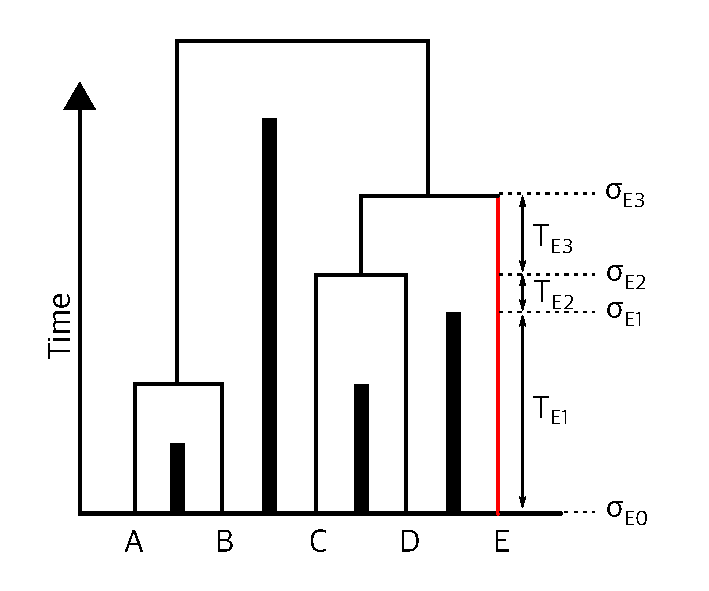
\includegraphics[width=0.6\textwidth]{genealogy_ebranch.pdf}
%	\caption{Sample figure caption.}
%	\label{fig:fig1}
%\end{figure}

%\subsection{Tables}
%See awesome Table~\ref{tab:table}.

%The documentation for \verb+booktabs+ (`Publication quality tables in LaTeX') is available from:
%\begin{center}
%	\url{https://www.ctan.org/pkg/booktabs}
%\end{center}


%\begin{table}
%	\caption{Sample table title}
%	\centering
%	\begin{tabular}{lll}
%		\toprule
%		\multicolumn{2}{c}{Part}                   \\
%		\cmidrule(r){1-2}
%		Name     & Description     & Size ($\mu$m) \\
%		\midrule
%		Dendrite & Input terminal  & $\sim$100     \\
%		Axon     & Output terminal & $\sim$10      \\
%		Soma     & Cell body       & up to $10^6$  \\
%		\bottomrule
%	\end{tabular}
%	\label{tab:table}
%\end{table}

%\subsection{Lists}
%\begin{itemize}
%	\item Lorem ipsum dolor sit amet
%	\item consectetur adipiscing elit.
%	\item Aliquam dignissim blandit est, in dictum tortor gravida eget. In ac rutrum magna.
%\end{itemize}


\bibliographystyle{ecol_let}
\bibliography{references}  

%%% Uncomment this line and comment out the ``thebibliography'' section below to use the external .bib file (using bibtex) .


%%% Uncomment this section and comment out the \bibliography{references} line above to use inline references.
% \begin{thebibliography}{1}

% 	\bibitem{kour2014real}
% 	George Kour and Raid Saabne.
% 	\newblock Real-time segmentation of on-line handwritten arabic script.
% 	\newblock In {\em Frontiers in Handwriting Recognition (ICFHR), 2014 14th
% 			International Conference on}, pages 417--422. IEEE, 2014.

% 	\bibitem{kour2014fast}
% 	George Kour and Raid Saabne.
% 	\newblock Fast classification of handwritten on-line arabic characters.
% 	\newblock In {\em Soft Computing and Pattern Recognition (SoCPaR), 2014 6th
% 			International Conference of}, pages 312--318. IEEE, 2014.

% 	\bibitem{hadash2018estimate}
% 	Guy Hadash, Einat Kermany, Boaz Carmeli, Ofer Lavi, George Kour, and Alon
% 	Jacovi.
% 	\newblock Estimate and replace: A novel approach to integrating deep neural
% 	networks with existing applications.
% 	\newblock {\em arXiv preprint arXiv:1804.09028}, 2018.

%\end{thebibliography}



%%%%%%%%%%%%%%%%%%%%%%%%%%%%%%%%%%%%%%%%%%%%%%%%%%%%%%%%%%%%%%%%%%%%%%%%%%%
%%%%%%%%%%%%%%%%%%%%%%%%%%%%%%%%%%%%%%%%%%%%%%%%%%%%%%%%%%%%%%%%%%%%%%%%%%%
%%%%%%%%%%%%%%%%%%%%%%%%%%%%%%%%%%%%%%%%%%%%%%%%%%%%%%%%%%%%%%%%%%%%%%%%%%%
%%%%%%%%%%%%%%%%%%%%%%%%%%%%%%%%%%%%%%%%%%%%%%%%%%%%%%%%%%%%%%%%%%%%%%%%%%%
%%%%%%%%%%%%%%%%%%%%%%%%%%%%%%%%%%%%%%%%%%%%%%%%%%%%%%%%%%%%%%%%%%%%%%%%%%%
%%%%%%%%%%%%%%%%%%%%%%%%%%%%%%%%%%%%%%%%%%%%%%%%%%%%%%%%%%%%%%%%%%%%%%%%%%%
%%%%%%%%%%%%%%%%%%%%%%%%%%%%%%%%%%%%%%%%%%%%%%%%%%%%%%%%%%%%%%%%%%%%%%%%%%%



\newpage

\beginsupplement
\section{Supplementary Information}

\setcounter{equation}{0}
\renewcommand{\theequation}{S\arabic{equation}}

\subsection{Supplementary Figures}

\begin{figure}[p]
	\centering
	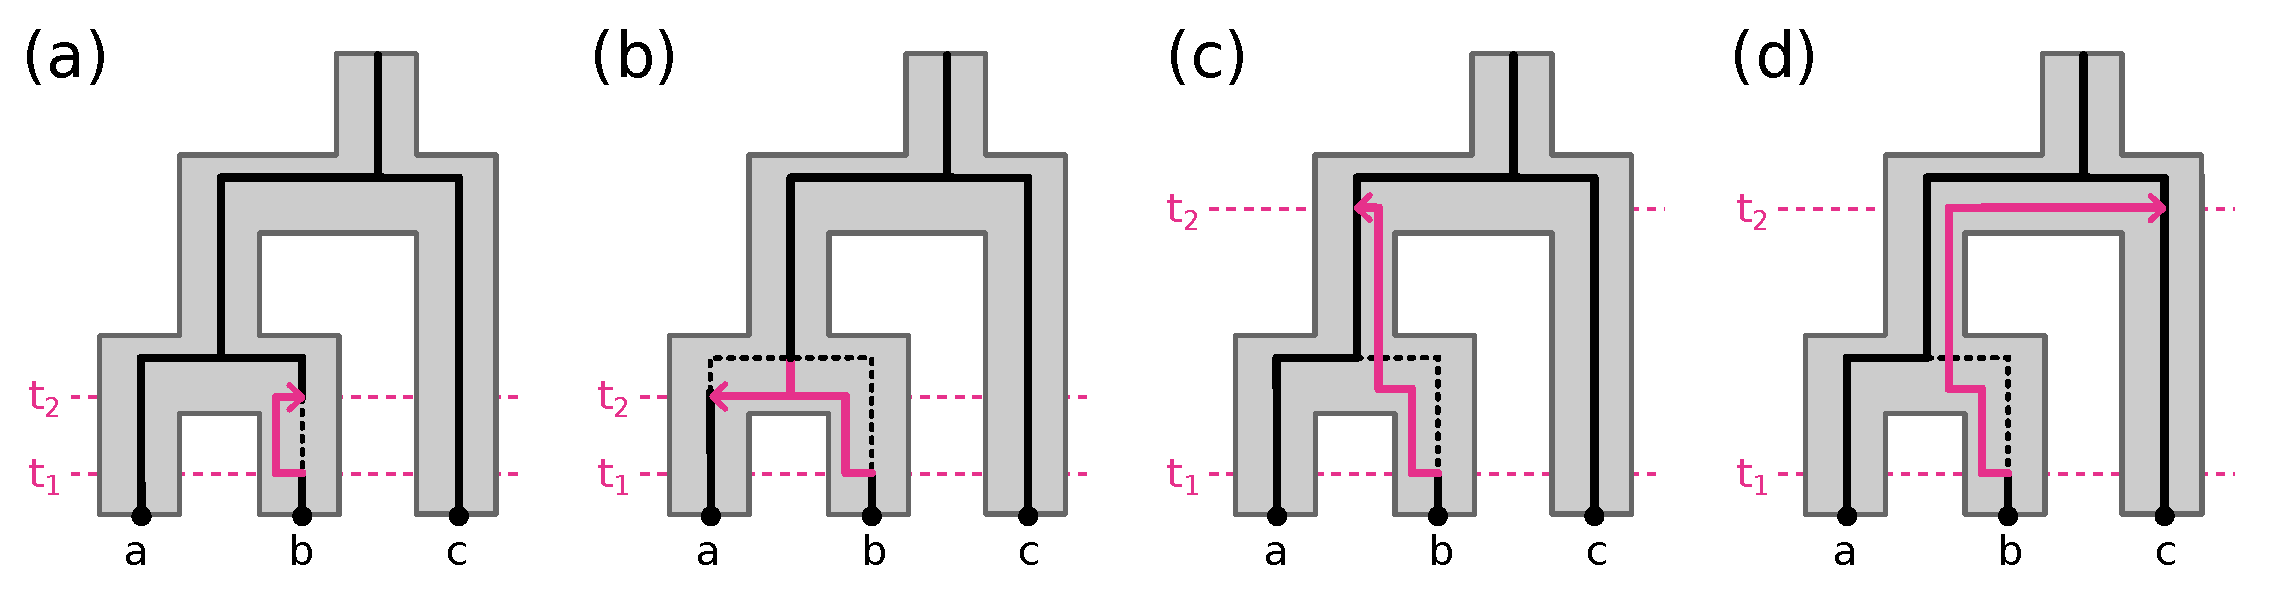
\includegraphics[width=0.9\textwidth]{figures/current/FigS1-recomb-types.pdf}
	\caption{
		Four categories of outcomes from a recombination event occurring on a
		%genealogy at time t$_1$ and the detached subtree re-coalescing with
		genealogy at time t$_1$, dictated by random subtree re-coalescence with
		a remaining lineage under the SMC' process at time t$_2$. (a) The
		detached subtree re-coalesces with the original lineage from which it
		was detached, leading to no change between the starting genealogy and 
		subsequent genealogy. (b) The detached subtree re-coalesces with its
		sibling lineage prior to their previous coalescence, leading to a shortening
		of their coalescence time. (c) The detached subtree re-coalesces with
		its parent lineage, leading to a lengthening of the coalescent time 
		between the detached subtree lineage and its sibling lineage. (d) The
		detached subtree re-coalesces with a lineage other than itself, its sibling,
		or its parent lineage, leading to a topology-change. 
	}
     \label{fig:figS-recomb-types}
\end{figure}

% \begin{landscape}
	% 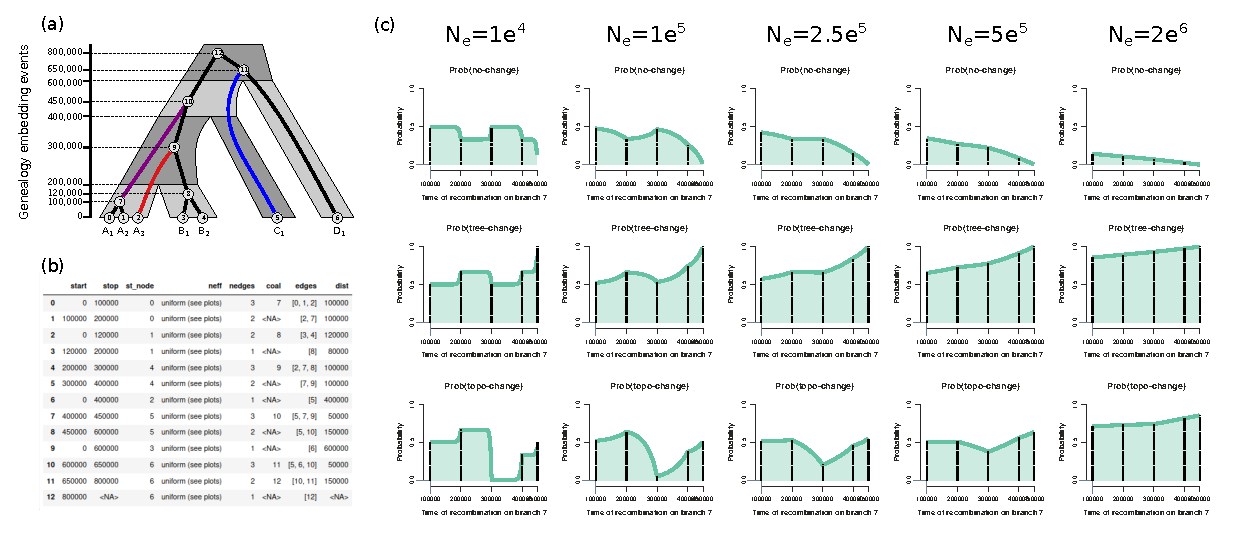
\includegraphics[width=0.99\linewidth,keepaspectratio]{figures/Fig-S2-edge-probabilities.pdf}
% \end{landscape}

\begin{figure}[p]
	\centering
	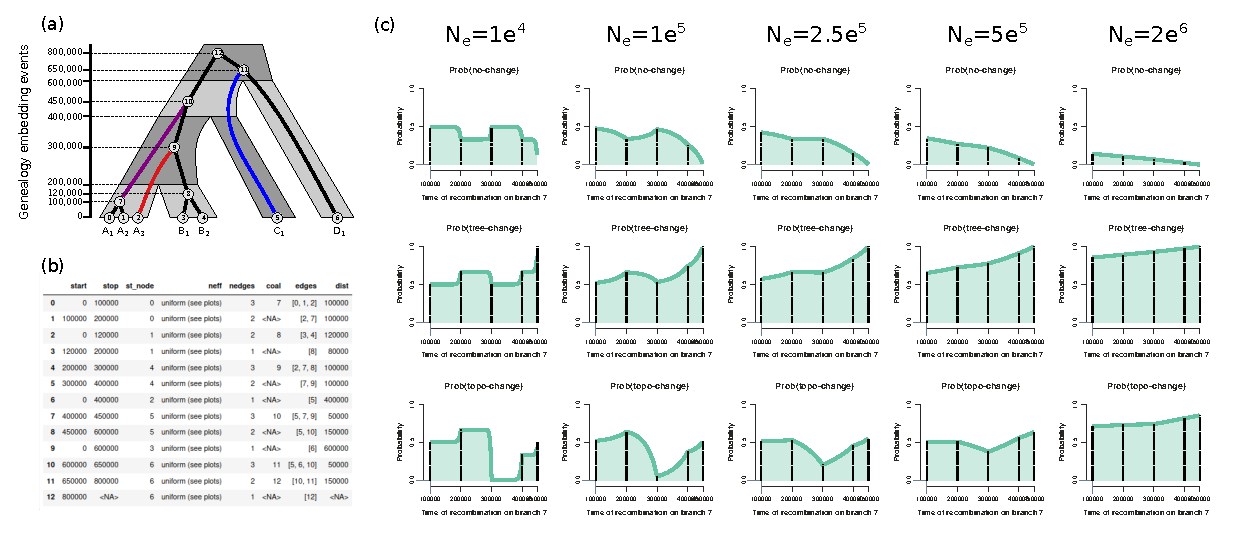
\includegraphics[width=0.99\textwidth]{figures/Fig-S2-edge-probabilities.pdf}	
	\caption{
		Probabilities of different recombination event outcomes for a selected 
		genealogy edge as a function of the time at which recombination occurs 
		and of the constant effective population size.
		(a) An MSC model with edge lengths in units of generations and an example
		genealogy embedded. (b) An genealogy embedding table for the example MSC
		model and genealogy. (c) Probabilities of different recombination event
		outcomes across genealogy edge 7. When $N_e$ is low, probabilities are 
		nearly constant with respect to time within each interval since re-coalescence in later intervals
		is unlikely. When $N_e$ is high, probabilities change nearly monotonically 
		across the length of an edge since population structure does little
		to constrain the time of re-coalescence.
	}
     \label{fig:figS-edge-probabilities}
\end{figure}


\begin{figure}[p]
	\centering
	% 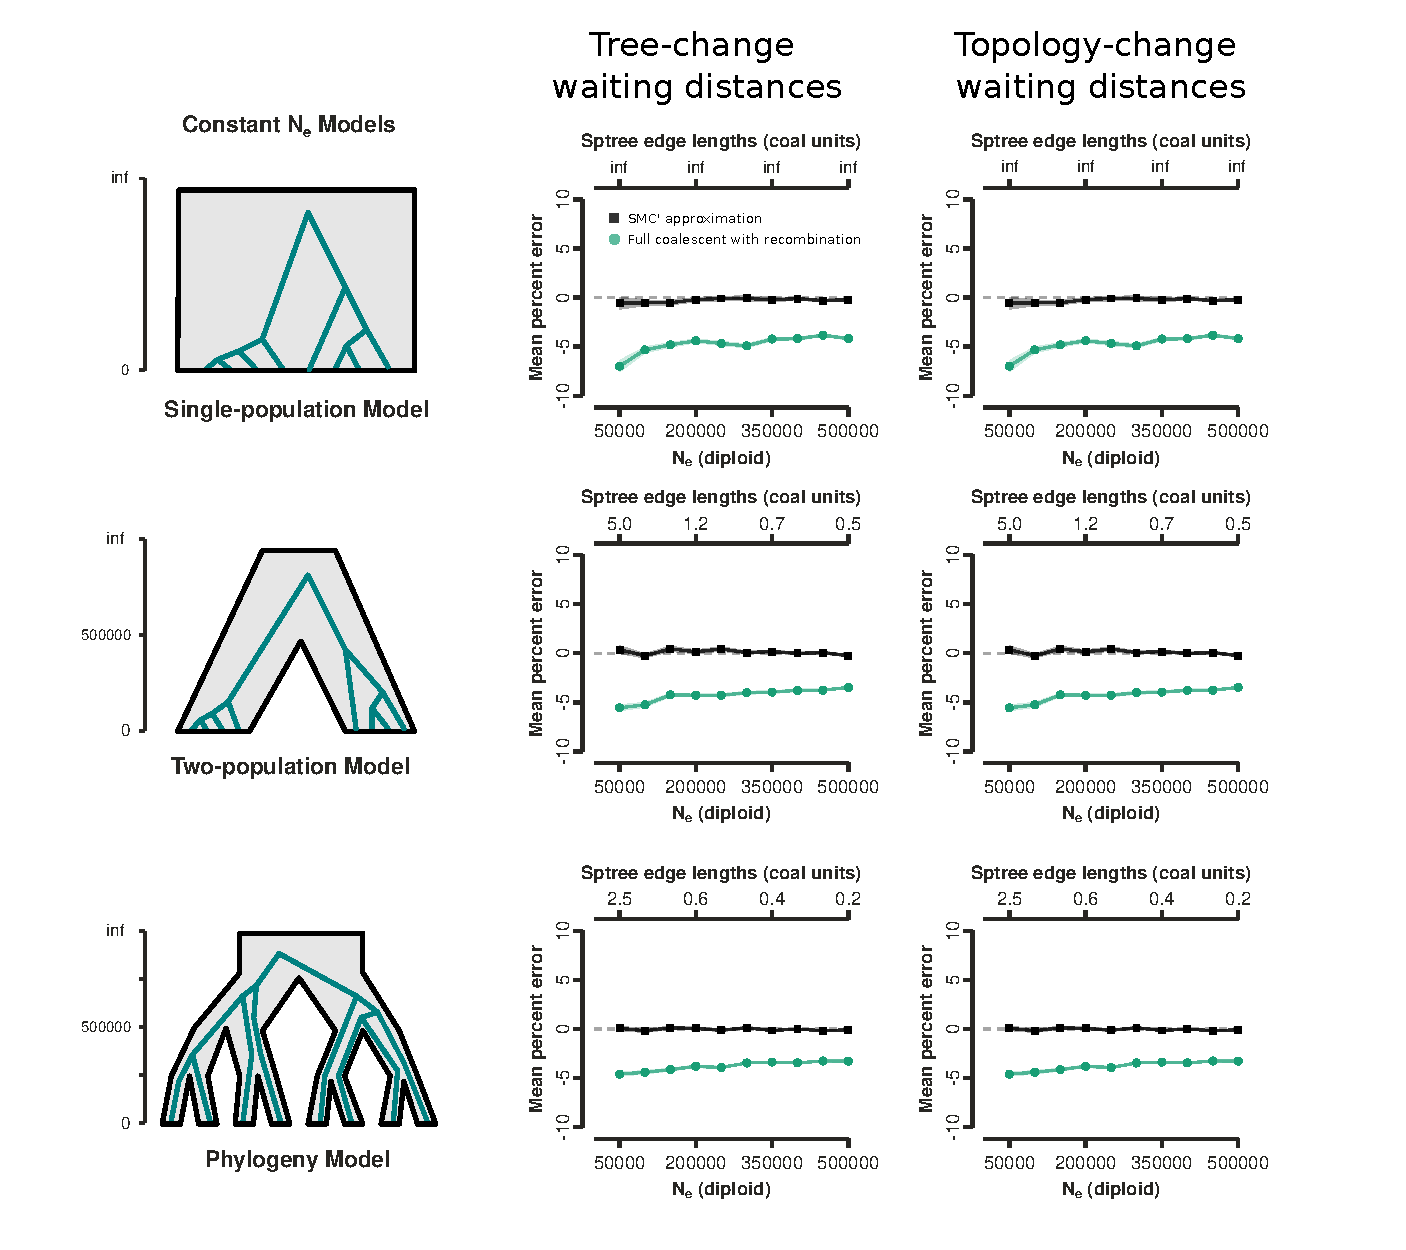
\includegraphics[width=0.99\textwidth]{figures/error-smc-approx.pdf}
	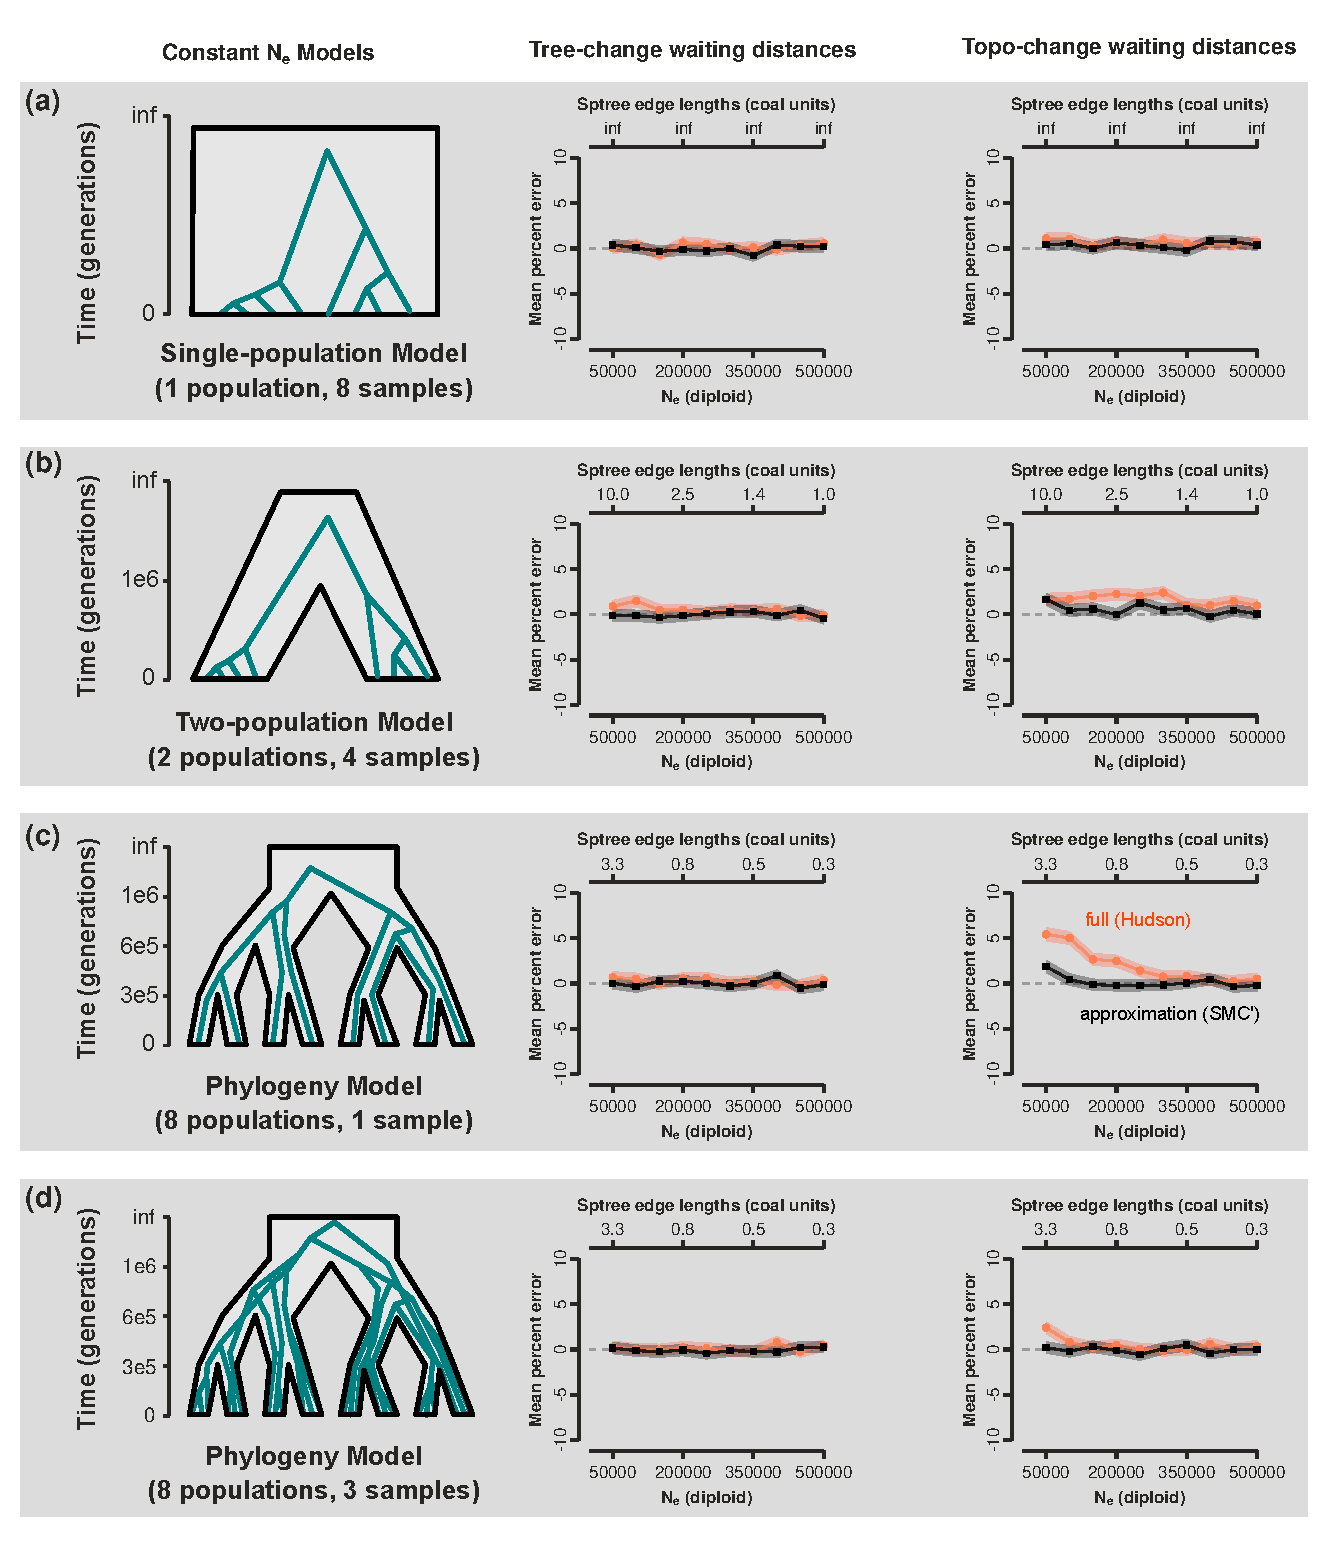
\includegraphics[width=0.79\textwidth]{figures/current/FigSY-smc-approx-bias.pdf}	
	\caption{
		\textcolor{red}{
		Error in the expected waiting distances to tree or topology-change events 
		calculated under the MS-SMC.
		Error was measured as (observed - expected) / expected, where observed is the 
		spanning distance of the first genealogy in a tree sequence until the next 
		tree or topology-change event, and expected is the predicted waiting distance
		for the first genealogy until each event type given its embedding in the 
		species tree model.
		Tree sequences were simulated for different demographic models across a range 
		of parameter settings for $N_e$, and under two different ancestry models
		(SMC'=black; full coalescent with recombination (Hudson)=orange).
		(a-d) Estimated tree-change waiting distances exhibit very little error across
		all models and parameters tested. Estimated topology-change waiting distances
		exhibit elevated error at low $N_e$ values in highly structured models, when
		the probability of a topology-change event is very low.
		(c) The error between analytical predictions and simulated data was greatest 
		when the data were simulated under the full coalescent with recombination. The
		(d) When more genomes are sampled per lineage the magnitude of error is greatly
		reduced.
		}
		% 
		% Error was measured as the mean percent difference between expected waiting distances
		% calculated under the MS-SMC and observed waiting distances in stochastic coalescent
		% simulations. Simulations were performed under both the SMC' approximation (black)
		% and the full coalescent with recombination (orange).
		% The difference in error between data simulated under these two models reveals the
		% impact of the SMC' approximation on MS-SMC inference.
		% Estimated tree-change waiting distances exhibit very little error in all datasets.
		% By contrast, estimated topology-change waiting distances exhibit greater
		% error, especially at low Ne values in the species tree model (c), where
		% topology-change events are very unlikely. When additional samples 
		% are added to each lineage in the species tree model (d) the error in MS-SMC 
		% estimates of topology-change waiting distances is greatly reduced.
		% This suggests that errors in the MS-SMC introduced by the SMC' approximation
		% can generally be avoided by sampling >1 genome per lineage in demographic models.}
		% \textcolor{red}{
		% \sout{
		% Error in MS-SMC’ waiting distance expectations caused by the SMC’ approximation. Error
		% was measured as the mean percent difference between expected waiting distances calculated under the MS-
		% SMC’ and observed waiting distances in stochastic coalescent simulations. Simulations were performed
		% under either the SMC’ approximation (black) or the full coalescent with recombination (green). The
		% MS-SMC’ tends to under-estimate waiting distances compared to the full coalescent with recombination,
		% but shows only a slight bias at very low N e values compared to simulations under the SMC’.
		% }}
	}
	\label{fig:figS-bias-smc}
\end{figure}



\begin{figure}[p]
	\centering
	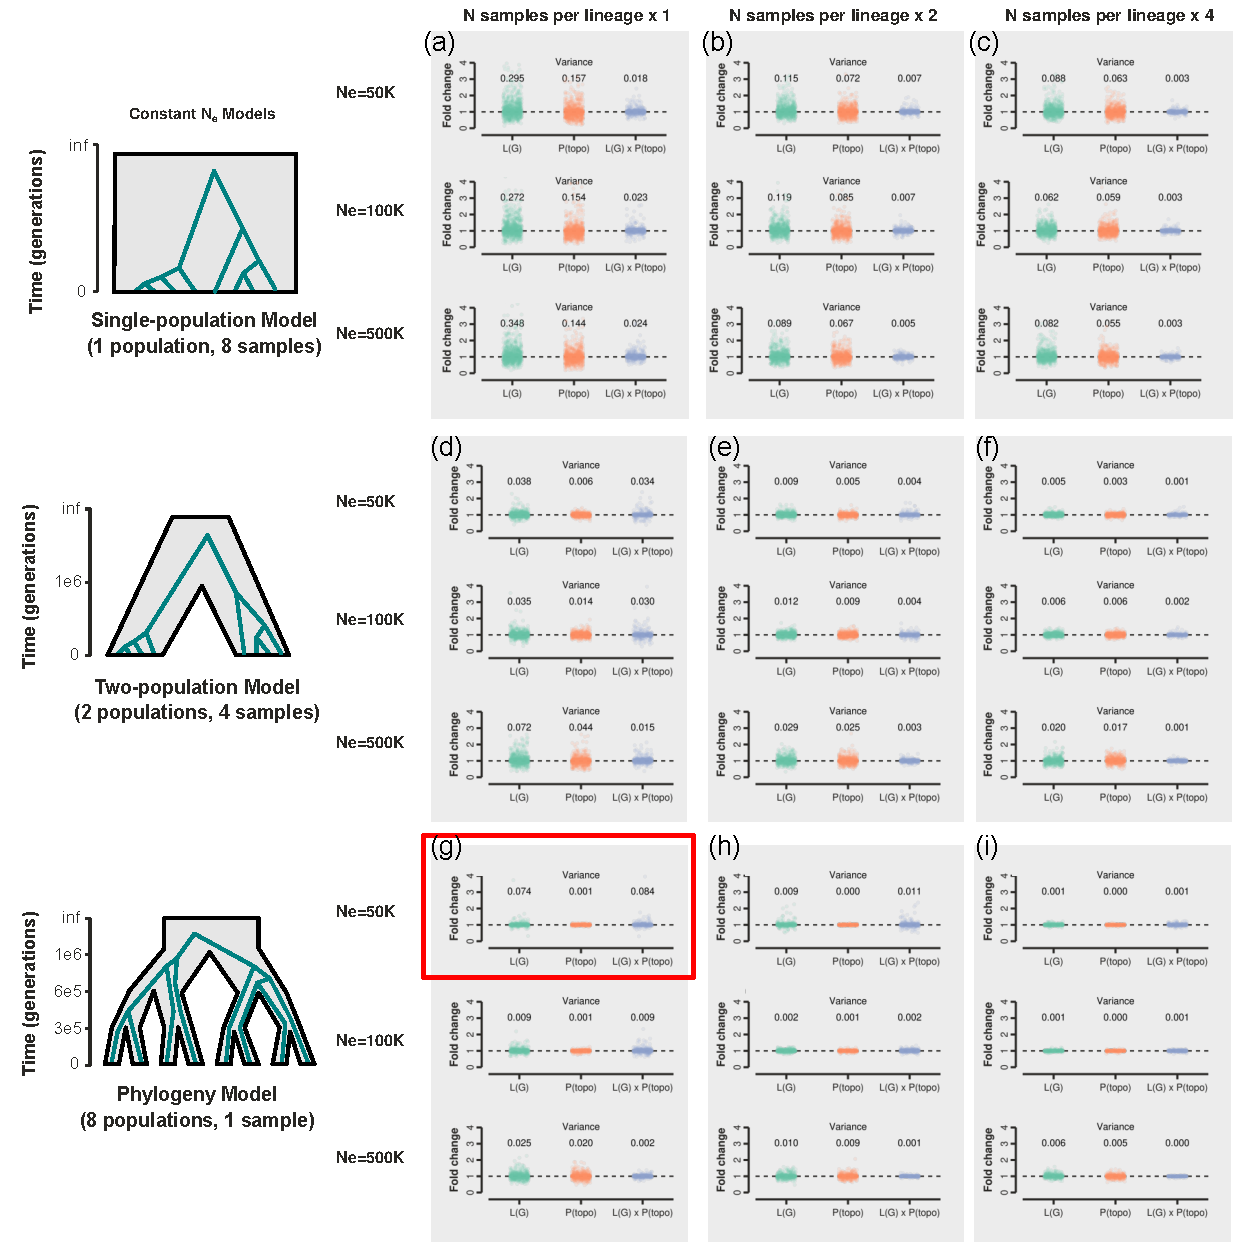
\includegraphics[width=0.99\textwidth]{figures/current/FigS-bias-fold-topo-first-2.pdf}
	\caption{
		\textcolor{red}{
		Variation between the first and second genealogies within topology-change 
		intervals, and its impact on estimated waiting distances.
		Results are shown for 1K tree sequences simulated across a range of 
		demographic models, $N_e$ values, and numbers of genomes sampled per lineage.
		% 
		For each scenario, plots show the distribution of fold-change differences
		between the first and second genealogies in summed edge lengths (L(G)),
		the probability of a topology change (P(topo)), and the product of these
		metrics. The variance is shown above each distribution.
		% 
		% (a-c) Fold-change difference between the first and second genealogies within
		% a topology-change interval for a single population model.
		(a-c) Single population demographic models consistently show high variance
		in the fold-change of each individual metric, but low variance in the
		fold-change of the product.
		(d-i) The two-population and phylogeny models typically exhibit less 
		variance, except in the lowest $N_e$ scenarios (e.g., red rectangle),
		where the product sometimes exhibits higher variance in fold-change.
		% more strongly with $N_e$ and the number of genomes sampled per lineage.
		% (g-i) The phylogeny model exhibits the least variance in L(G) and P(topo), 
		% and typically very low variance in their product. However, in the scenario
		% at the lowest $N_e$ value and number of samples per lineage (red rectangle),
		% the variance in the fold-change of their product is highest. 
		This suggests that the potential for tree-change events occurring within a 
		topology-change interval to bias estimates of the waiting distance to a
		topology-change, is only a concern in scenarios where topology-change events
		are very unlikely. (e,g,h,i) Sampling more genomes per lineage greatly 
		reduces this bias.
		}
		% % OLD FIGURE LEGEND
		% Variance in the fold-change for components affecting the expected waiting 
		% distance to a topology-change event between the starting tree and a subsequent
		% tree which has experienced a tree-change event, changing the coalescent times
		% but not the topology. The sum of genealogical edge lengths (L(G)), the 
		% P(topology-change | S,G), and the product of these two terms are shown for
		% three different demographic models and
		% \textcolor{red}{\sout{with} at} different constant $N_e$ values, 
		% and numbers of samples per lineage.
		% When the fold-change in the product exhibits low variance around 1 the 
		% MS-SMC approximation for the expected waiting distance until a topology-change 
		% is expected to be more accurate. Larger effective population sizes and 
		% numbers of samples per lineage yield lower variance in the product.
	}
     \label{fig:figS-bias-topo-first}
\end{figure}


\begin{figure}[p]
	\centering
	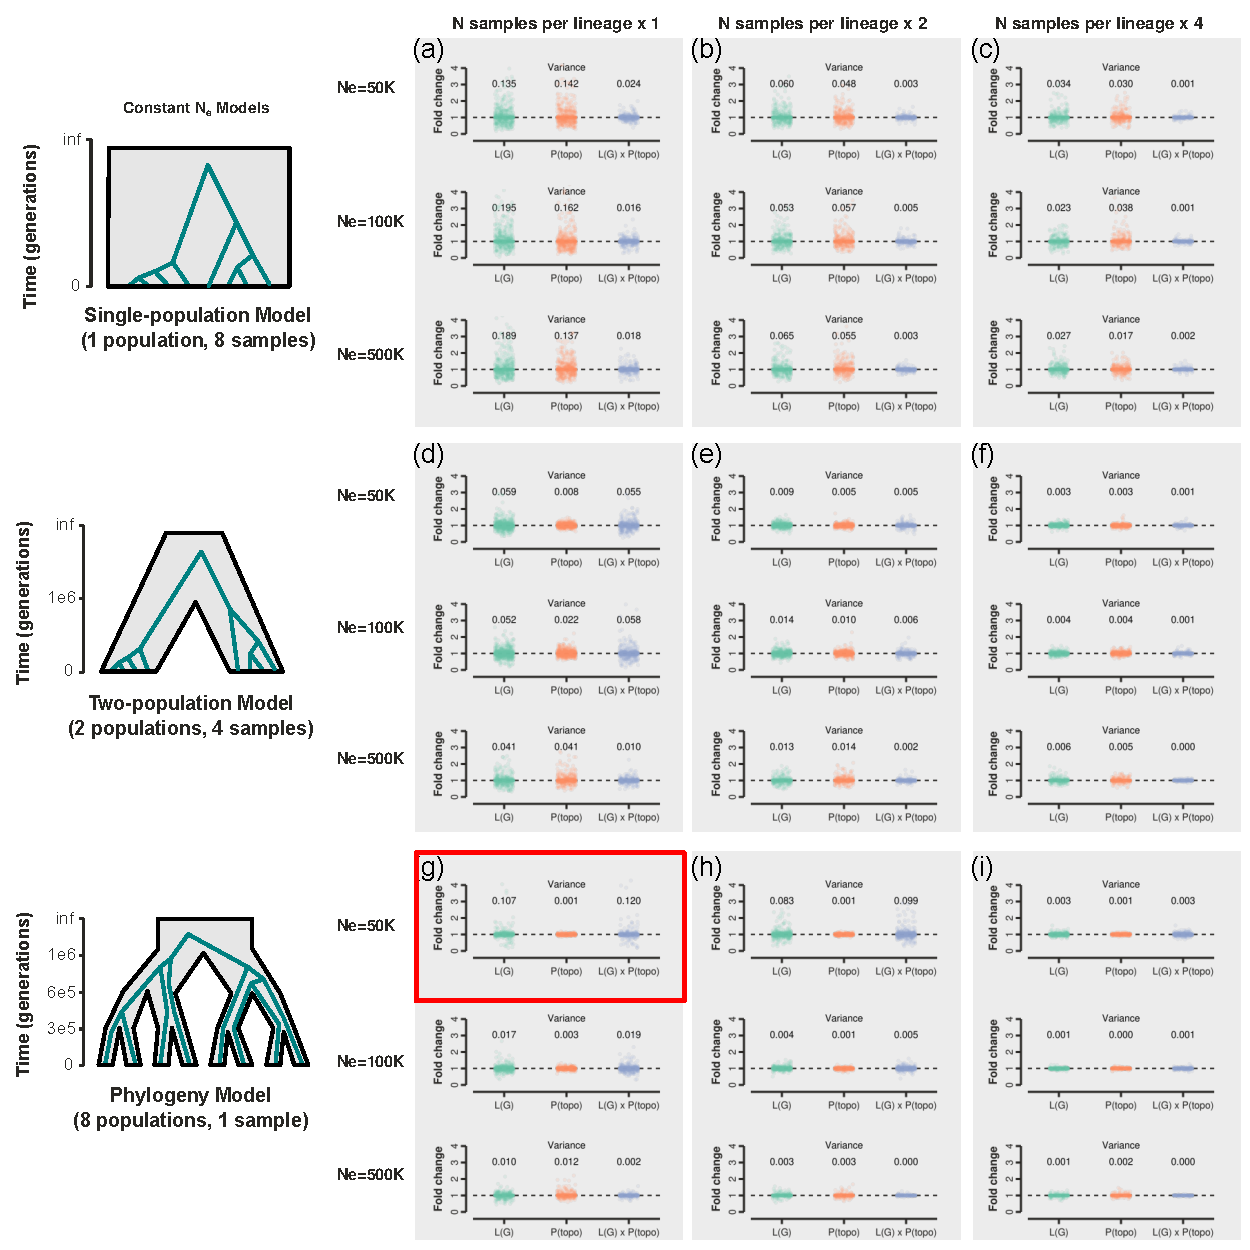
\includegraphics[width=0.99\textwidth]{figures/current/FigS-bias-fold-topo-last-2.pdf}
	\caption{
		\textcolor{red}{
		Variation between the first and last genealogies within topology-change 
		intervals, and its impact on estimated waiting distances.
		Results are shown for 1K tree sequences simulated across a range of 
		demographic models, $N_e$ values, and numbers of genomes sampled per lineage.
		% 
		For each scenario, plots show the distribution of fold-change differences
		between the first and last genealogies in summed edge lengths (L(G)),
		the probability of a topology change (P(topo)), and the product of these
		metrics. The variance is shown above each distribution.
		% 
		(a-c) Single population demographic models consistently show high variance
		in the fold-change of each individual metric, but low variance in the
		fold-change of the product.
		(d-i) The two-population and phylogeny models typically exhibit less 
		variance, except in the lowest $N_e$ scenarios (e.g., red rectangle),
		where the product sometimes exhibits higher variance in fold-change.
		% 
		This suggests that the potential for tree-change events occurring within a 
		topology-change interval to bias estimates of the waiting distance to a
		topology-change, is only a concern in scenarios where topology-change events
		are very unlikely. (e,g,h,i) Sampling more genomes per lineage greatly 
		reduces this bias.		
		}
		% OLD FIGURE LEGEND
		% Variance in the fold-change for components affecting the expected waiting 
		% distance to a topology-change event between the starting tree and a subsequent
		% tree which has experienced a tree-change event, changing the coalescent times
		% but not the topology. The sum of genealogical edge lengths (L(G)), the 
		% P(topology-change | S,G), and the product of these two terms are shown for
		% three different demographic models and
		% \textcolor{red}{\sout{with} at} different constant $N_e$ values, 
		% and numbers of samples per lineage.
		% When the fold-change in the product exhibits low variance around 1 the 
		% MS-SMC approximation for the expected waiting distance until a topology-change 
		% is expected to be more accurate. Larger effective population sizes and 
		% numbers of samples per lineage yield lower variance in the product.
	}
     \label{fig:figS-bias-topo-last}
\end{figure}




\begin{figure}[p]
	\centering
	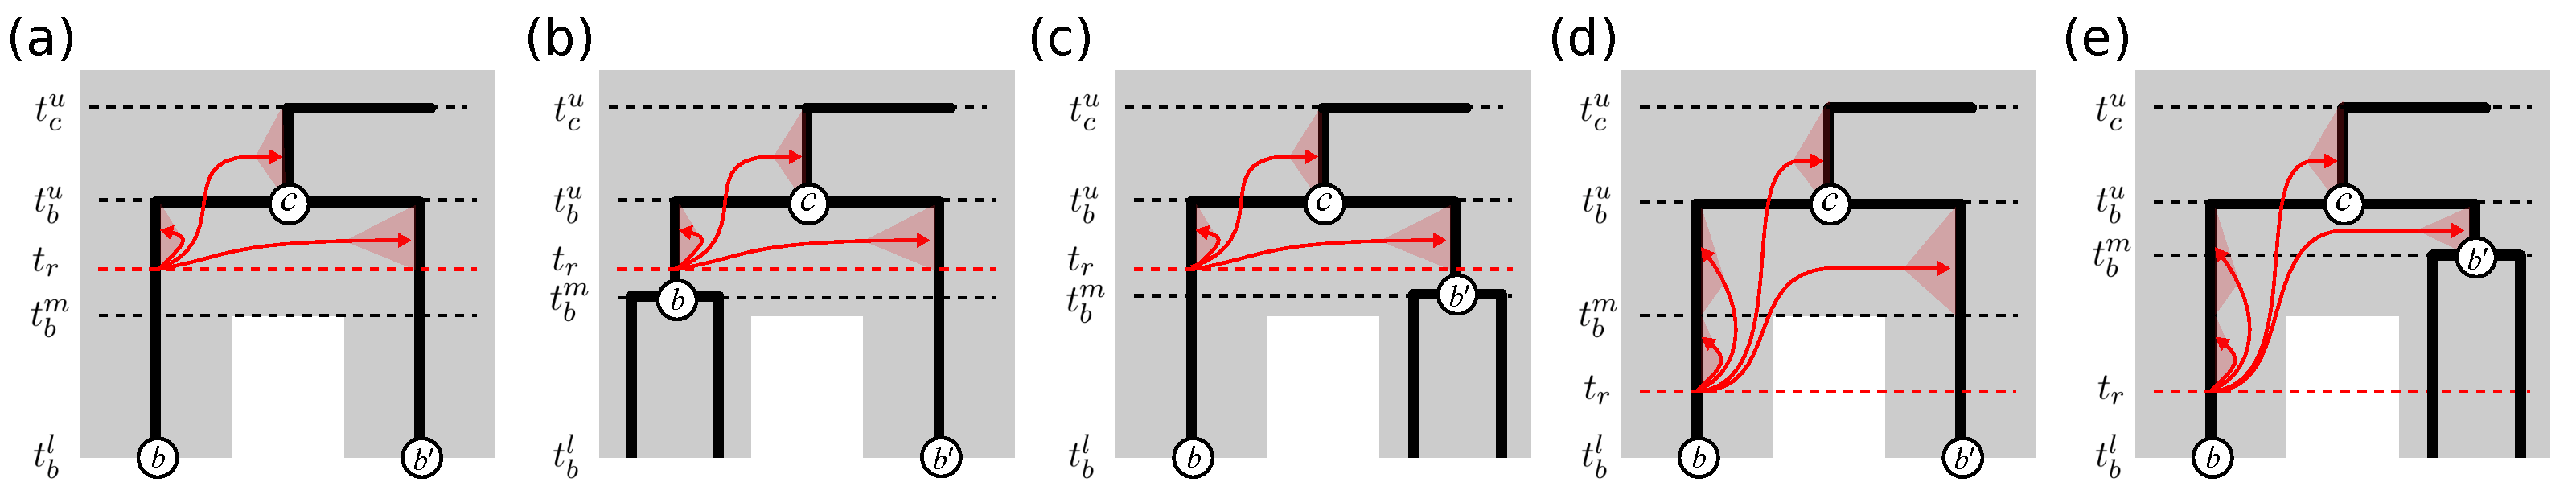
\includegraphics[width=0.95\textwidth]{figures/FigS-tbm.pdf}
	\caption{
		Calculating the probability that recombination on genealogy branch 
		$b$ leads to a topology change involves summing over the probabilities 
		that the detached lineage does not re-coalesce with either
		itself, its sibling, or its parent ($b$, $b'$ or $c$, respectively). 
		The possibility of a tree-change outcome (e.g., shortened coalescent 
		time) is restricted until the lowest shared interval between $b$ and 
		$b'$, designated at time $t_m$. Opportunities for such events could be
		constrained by species divergences -- as in (a) and (d) -- or by the timing of 
		prior coalescence events generating each branch -- as in (b), (c), and (e). 
		The possibility that recombination ($t_r$) occurs prior
		to $t_m$ leads to the two ordered sets of intervals used in 
		equations 11 and 12.
		%When the timing of recombination ($t_r$) \hl{occ...}
		%$b$ and $b'$ can either exist 
		%in different species tree intervals (a) or the same interval (b). This 
		%restricts the probability of tree-change outcomes (e.g., shortened coalescent 
		%time) until the lowest shared interval between $b$ and $b'$ at time 
		%$t_m$, leading to the two ordered sets of intervals (c-d) used in 
		%equations 11 and 12.
	}
	\label{fig:figS-tbm}
\end{figure}


\begin{figure}[p]
	\centering
	\includegraphics[width=0.95\textwidth]{figures/current/FigS6-equations}
	\caption{A step-by-step calculation of the probability of a tree-unchanged 
	event under the MS-SMC given a species tree and genealogy.
	}
	\label{fig:figS-tree-equations}
\end{figure}


\begin{figure}[p]
	\centering
	\includegraphics[width=0.95\textwidth]{figures/current/FigS7-equations-topo}
	\caption{A step-by-step calculation of the probability of a topology-unchanged 
	event under the MS-SMC given a species tree and genealogy.
	}
	\label{fig:figS-topo-equations}
\end{figure}


\begin{table}[p]
\centering
\caption{\label{tab:table-notation} 
	Summary of variables used in waiting distance equations. 
}
\begin{tabular}[t]{ |c|l| }
	\toprule
	Variable & Description \\
	\midrule
	$\mathcal{S}$    & An MSC model with topology, divergence times and effective population sizes. \\
	$\mathcal{G}$    & A genealogy that can be embedded in $\mathcal{S}$. \\
	$L(\mathcal{G})$ & Sum of edge lengths of genealogy $\mathcal{G}$. \\
	$b$ 			  & A focal branch in $\mathcal{G}$. \\
	$i$              & Interval in the genealogy embedding table in which recombination occurs.\\
	$\mathcal{I}_b$  & Ordered set of intervals on branch $b$.\\
	$\mathcal{I}_{c}$   & Ordered set of intervals on branch $c$, the parent of branch $b$.\\
	$\mathcal{I}_{bc}$  & Ordered union of sets $\mathcal{I}_{b}$ and $\mathcal{I}_{c}$.\\
	$\mathcal{J}_b(i)$  & Ordered set of intervals above $i$ on branch $b$.\\	
	$\mathcal{Q}_b(i,j)$ & Ordered set of intervals above $i$ and below $j$ on branch $b$.\\
	$\mathcal{K}(b,t)$ & Number of edges of $\mathcal{G}$ in the interval containing branch $b$ at time $t$.\\
	$k_x$              & Number of edges of $\mathcal{G}$ in interval $x$; piece-wise constant of $A(b,t)$.\\
	$\mathcal{N}(b,t)$ & Diploid effective population size in the interval containing branch $b$ at time $t$.\\
	$n_x$              & Diploid effective population size in interval $x$; piece-wise constant of $N(b,t)$. \\
	$t_r$		& Time of a recombination event, in generations. \\
	$\sigma_x$     & The lower boundary of interval $x$, in generations. \\
	$\mu_x$        & The upper boundary of interval $x$, in generations. \\	
	$d_x$          & The length of interval $x$, in generations. \\
	$t_b^l$        & The lower boundary of branch $b$, in generations. \\
	$t_b^u$        & The upper boundary of branch $b$, in generations. \\
	$t_b^m$        & The time at which a focal branch $b$ is able to coalesce with its sibling branch. \\
	% $m$            & Index of an interval in the genealogy embedding table with lower boundary $t_b^m$. \\
	$\mathcal{M}_b$  & Ordered set of intervals above $t_b^m$ on branch $b$.\\
	$\mathcal{L}_b$  & Ordered set of intervals below $t_b^m$ on branch $b$.\\	
	% $\mathcal{I}_b$  & The number of intervals containing branch $b$. \\
	\bottomrule
\end{tabular}
\end{table}



\newpage


% \section{Appendix: Derivations}
% \subsection{Derivations of the Multispecies Sequentially Markov Coalescent (MS-SMC)}


% \subsection{testing}

% and also act in opposing directions, such that their
% combined effect is further reduced.

% The MS-SMC’ harbors two potential sources of bias. The first affects only 
% topology-change waiting distances, and appears to have a relatively small effect. 
% This stems from the potential for topology-change probabilities to vary spatially
% across a distance of the genome between two topology-change events as a result 
% of intermediate tree-change events 
% (e.g., the second and third recombination events in Fig.~\ref{fig:fig2}).
% Consequently, unlike the exact solution for tree-change waiting distances, 
% topology-change waiting distances represent an approximation. 
% Using  coalescent simulations we measured the variance in probabilities of 
% topology-change across the spanned intervals between topology-change 
% events (Supplemental Materials for methods and results; Fig.~\ref{fig:figS-bias-topo}).
% Multispecies models do not exhibit greater error than single population models.
% A second source of bias stems from assumptions of the SMC’ approximation to the full 
% coalescent with recombination model. By not modeling recombination events that 
% occurred among ancestors that do not contribute genetic material
% to the samples, SMC'-based methods tend to under-estimate recombination events. 
% The frequency of such events in single populations is small \citep{mcvean2005approximating}. 
% We performed coalescent simulations to examine how this error increases in multi-species models 
% (see Supplemental Materials for methods), and found that our MS-SMC estimations exhibit 
% almost no error when compared to data simulated under the SMC' process, but approximately
% -5\% compared to the full coalescent with recombination model (Fig.~\ref{fig:figS-bias-smc}). 

% ....
% ...
% A second source of error affects only topology waiting distances. ...
% he SMC’ approximation to the coalescent with recombination is expected to deviate more signifi-
% cantly from the full model that it is approximating as the number of recombination events that the SMC’
% does not model (among ancestors that do not contribute genetic material to sampled descendants) increases.
% By not modeling some recombination events the SMC’ will tend to over-estimate waiting distances be-
% tween tree or topology change events.

% and the second from the approximate 
% nature of waiting distance estimation for topology-change events. We examined both 
% of these sources of error through comparison to stochastic simulations
% and found that their effects are generally negligible, and also act in opposing directions, such that their
% combined effect is further reduced.

% % now present the caveats...
% This final expectation comes with an important caveat. 
% % does come with a caveat. 


% % more complicated, % to derive, 
% % waiting distance distribution to a \emph{topology} change is more 
% % solution for a \emph{topology} change is more complicated, % to derive, 
% % due to the possibility of intermediate recombination events 
% % because of the possibility of intermediate recombination events 
% % that change branch lengths but not the topology 

% % In other words, during the waiting distance until a topology-change occurs,
% % given a specific starting genealogy, the genealogy branch lengths could 
% % change, thus affecting the probabilities of subsequent outcomes.
% % subsequent recombination events, 
% % including the relative probabilities of different categorical types.
% % for the next event.
% % As these events
% % As the branch lengths of intermediate genealogies change this affects the
% % rate of subsequent recombination events, and thus 
% % These events impact the rate of recombination events and 
% % the probability
% % that each further recombination event changes
% % that such events could change
% % the topology of the %newly generated 
% % next
% % genealogy. 
% % This problem was first described by \citet{deng_distribution_2021},
% % who previously demonstrated that its effect can likely be ignored. 
% Another potential source of error is the SMC' approximation itself, 
% which excludes recombination events 
% restricting re-coalescence to only occur with 



% We re-examined this potential bias in the context of MSC models 
% (Supplementary Materials 5.2) and found a similar result, 
% with MSC models in fact exhibiting less spatial variation in 
% topology-change probabilities than single population models, and 
% thus less error. We also examined potential bias in waiting distance 
% expectations that may arise from the SMC' approximation 
% (Supplementary Information 5.2), where MSC models also exhibit less 
% error than single population models, owing to their lower variance 
% in tree and topology-change probabilities.

%\subsection{Implementation of theoretical results}

%\textcolor{red}{* get a species tree and gene tree
%* decompose into the embedding table
%* implement each of the key equations
%* visualize results
%Describe using these to generate the likelihood solutions.}

\subsection{Investigating bias in MS-SMC predictions}
% in addition to SMC' approximation, topo-change has additional bias.
The MS-SMC harbors two potential sources of bias, the first stemming from 
assumptions of the SMC' approximation and the second from the 
\textcolor{red}{potential inhomogeneity among genealogies that can exist 
between topology-change events}.
% REMOVED
\textcolor{red}{\sout{approximate 
nature of waiting distance estimation for topology-change events}}
% 
We examined both of these sources of error through comparison to stochastic
simulations and found that their effects are generally negligible,
% ADDED THIS
\textcolor{red}{and that structured demographic models do not exhibit 
greater error than a single-population model under most scenarios.}
% REMOVED THIS
\textcolor{red}{\sout{and act in opposing 
directions such that their combined effect is further reduced.}}


\subsubsection{Bias associated with the SMC' approximation}
% MOVED THIS SENTENCE TO OCCUR EARLIER
%% "exhibit" here because SMC' per se isn't estimating anything
%Because our waiting distance predictions are built upon assumptions of 
%the SMC' model, they too will exhibit this bias. 
% Models with high population structure, such as MSC models with low Ne, 
% where many recombination events
% could occur among samples deep in time, but contribute no genetic material
% to samples at the present. 
To investigate 
\textcolor{red}{
the extent to which the SMC' approximation leads to errors in waiting
distance estimation, 
\sout{this source of error in our waiting distance predictions,}
we repeated the simulations from our validation scenario using the SMC'
model (msprime setting "ancestry\_model=smc\_prime") as opposed to the 
full coalescent with recombination model ("ancestry\_model=hudson") that
we used previously.
}
\sout{\emph{msprime} setting "ancestry\_model=smc\_prime" to simulate tree sequences 
that only retain recombination events that would occur in the SMC' model.
}
% 
\textcolor{red}{
We expect that waiting distances in simulations under the SMC' will match 
our analytical predictions more closely than the waiting distances in 
simulations under the full coalescent with recombination, since our MS-SMC
model relies on the assumptions of the SMC'.
}
% \textcolor{red}{\sout{
% The SMC' approximation to the full coalescent with recombination is expected 
% to deviate increasingly far from the full model that it is approximating 
% as the number of recombination events that the SMC' does not model 
% (i.e., those that are among ancestors who do not contribute genetic 
% material to sampled descendants) increases. 
% }}
% ADDED
% REMOVED THIS
% By not modeling this subset of recombination events, the SMC' will tend to 
% exhibit greater waiting distances between tree or topology change events than the full model. 
% 
% ADDED THIS
% The SMC' approximation to the full coalescent with recombination performs
% more efficiently by not modeling the ancestry of samples that do not contribute
% genetic material to the sampled descendants. Therefore, we expect that when
% a greater proportion of the history of a sample does in fact contribute
% genetic material to the descendants, such as in low Ne scenarios, results
% from the SMC' approximation will deviate more significantly from the full
% model. 
% the sample includes a greater proportion
% % 
For each simulated tree sequence we calculated the expected waiting distance to 
a tree or topology-change event given the starting genealogy and species tree, 
and compared this to the observed waiting distance to each event type for the
starting genealogy in the simulation.
% 
We measured the percent error for each genealogy
\sout{The percent error in these analyses was measured}
as 100 $\times$ (simulated waiting distance - expected waiting distance) / expected waiting distance.
This was repeated across 100K tree sequences for each simulation setting, 
and the mean and standard error were calculated.

% 
The error in our analytical predictions was very low across all demographic
models and parameter settings tested, regardless of whether data were simulated
under the SMC' approximation or not
(Fig.~\ref{fig:figS-bias-smc}). 
% 
The mean percent error in estimated tree-change waiting distances 
rarely exceeded 1\%, while the error in estimated topology-change 
waiting distances varied depending on the demographic and simulation 
models.
% , and exhibited very little difference whether
% compared to the SMC' or full coalescent with recombination data.
% 
The error in estimated topology-change waiting distances was always
$<$5\% for data simulated under the SMC', and only exceeded 5\% in
one scenario tested for simulations under the full coalescent with
recombination. This scenario represents an extreme case, in the form of
a "Phylogeny Model" with only a single sample per species, and very low 
Ne, such that genealogical discordance is very low. This leads to very 
long expected waiting distances between topology events, and very high 
variance in the simulated outcomes (Fig.~\ref{fig:figS-bias-smc}c). 
By simply increasing the number of samples per lineage, such that 
topology-change events can occur not only between lineages, but also 
within them, this error is reduced to approximately 2\% for the full 
coalescent with recombination, and nearly zero for SMC' data 
(Fig.~\ref{fig:figS-bias-smc}d). 


Although tree-change waiting distances did not exhibit consistent errors,
the error in estimated topology-change waiting distances, when present,
was consistently in the direction of being under-estimated. The fact that
this bias is not observed in the distance to tree-change events, but only
for topology-change events, suggests that the SMC' approximation has
little effect on the accuracy of estimation for an individual genealogy,
but can lead to more detectable errors when compounded over many tree-change
events occurring between a topology-change event.
% 
In other words, the SMC' approximation does not introduce a significant
bias on its own, but does contribute to increased error in topology-change 
change waiting distances through its interaction with a second source of error,
the inhomogeneity of genealogies between topology-change events (examined
further below). 
% 
We expect that the reason this bias tends to occur in the direction
of under-estimated waiting distances to a topology-change is because 
the intervening tree-change events can cause the genealogy to enter a 
space where the probability of a topology-change is much less likely 
than it was on the tree at the start of the interval. 
% 


% \textcolor{red}{
% The error rate observed in the Phylogeny Model scenario is interesting
% in three respects: 
% (1) the difference between the full and SMC' data; (2) the effect of Ne;
% and (3) the direction of the bias. First, because both the full and SMC' data
% show an elevated error at the lowest Ne value, we believe that some but not 
% all of this error rate is actually caused by the SMC' approximation. This
% raises the question, why is the error greater at low Ne values? We believe
% that this is a consequence of a greater proportion of recombination events
% that 
% }

% than for topology-change waiting distances. The scenario with the
% greatest error involved topology-change weighting distances calculated in the
% "Phylogeny model" at very low Ne values (Fig.~\ref{fig:figS-bias-smc}c). Here 
% the error calculated for data simulated under the full model greatly exceeds 
% that for the SMC' model, although both increase at low Ne. 

% REMOVED
% \textcolor{red}{
% \sout{We have already seen from our validations that the error in our predictions 
% is quite low when data are simulated under the full coalescent with 
% recombination (Fig.~\ref{fig:figS-bias-smc}).
% }}
% When quantified, 
% As expected, we observe even less error 
% between our predictions and coalescent simulations when data are simulated
% under the SMC' model. 
% MODIFIED PERCANTAGE ERROR W/ NEW CALCULATION
% Whereas the error rate is generally below 
% \textcolor{red}{2\%}
% REAPLACED
% 5\% 
% 
% when data are simulated under the full coalescent
% with recombination model 
% % REPLACED
% \textcolor{red}{(only exceeding this in some very low Ne scenarios)}
% % (only exceeding this at the lowest
% % $N_e$ values examined) 
% mean error rates do not exceed 5\% in any 
% models for data simulated under the SMC' assumptions. 
% This shows that the SMC' assumption does contribute a relatively small error 
% to our waiting distance predictions, especially at low $N_e$ values,
% where it can lead to over-estimated waiting distances.

% % WHAT KIND OF SMC' bias did we observe
% \textcolor{red}{T}
% 
% HOW DO WE EXPLAIN THIS
%
%
% WHAT KING OF TOPO-CHANGE INHOMOGENEITY APPROX BIAS DO 
%
% REMOVE THIS\

\subsubsection{Bias associated with inhomogeneity between topology-change events}

To investigate the impact of genealogical variation within a topology-change interval
on the accuracy of its estimated waiting distance, we measured how much genealogies vary
within these intervals, and how much this impacts probabilities of topology-change.
% 
Because topology-change waiting distances are calculated based on the genealogy
at the start of an interval, we compared the first genealogy to both the second
and last genealogy in each interval.
% 
For each tree we calculated the genealogy length ($L(\mathcal{G})$), 
the probability of a topology-change given $\mathcal{G}$ and $\mathcal{S}$,
and the product of these two metrics, which equates to the waiting distance 
rate parameter (equations 7, 8, 10).
% 
\citet{deng_distribution_2021} noted that for a single population with constant $N_e$
there is an inverse relationship between genealogy length and the probability of a 
topology change, such that their product exhibits little variation even if genealogies
vary across an interval.
% 
It was not clear whether this is also true for an MSC model, since the embedding of
a genealogy into the species tree affects the probability of a topology change in 
addition to the edge lengths of the genealogy. 
% 


Therefore, we examined genealogical variation across three demographic models, 
at three different values for $N_e$, and for different numbers of genomes sampled
per population. We simulated 1,000 tree sequences for each scenario using the 
coalescent with recombination ancestry model. 
% 
For each tree sequence we extracted information from one topology-change interval. 
To select the interval we advanced to the first interval after the first topology-change 
event that included at least one tree-change event within it.
For this interval we measured $L(\mathcal{G})$, 
$\mathbb{P}(\textrm{topology-change}| \mathcal{S}, \mathcal{G})$ and their
product, for the first genealogy, second genealogy, and last genealogy in the interval.
We measured the fold-change for each variable between the first and second 
genealogies, and between the first and last genealogies.
% 


Across all simulations our results confirm and extend the conclusions of 
\citet{deng_distribution_2021}, showing that although $L(\mathcal{G})$ 
and $\mathbb{P}$ can both exhibit high variance in fold-change between the 
first and second genealogies in an interval (Fig.~\ref{fig:figS-bias-topo-first}), 
and between the first and last genealogies in an interval (Fig.~\ref{fig:figS-bias-topo-last}),
the product of these two metrics almost always exhibits lower variance in
fold-change, and is centered on one.
% 
In a single population model the variance in the fold-change of the product of
these two metrics was approximately 0.02, and did not vary with $N_e$, or 
depending on whether we compared the first and second, or first and last
trees in an interval. The variance in the product was reduced by nearly 
an order of magnitude when the number of genomes sampled was increased 
(Fig.~\ref{fig:figS-bias-topo-first}a-c,\ref{fig:figS-bias-topo-last}a-c).
We can conclude that genealogical heterogeneity has a very small effect
on estimated waiting distances to topology-changes in a single population model.

% 
In the two-population and phylogeny models the variance in the fold change of 
$L(\mathcal{G})$, $\mathbb{P}$, and their product was strongly affected by the
model $N_e$, and consistently smaller between the first and second genealogy, 
than between the first and last genealogy in an interval.
(Fig.~\ref{fig:figS-bias-topo-first}d-i,\ref{fig:figS-bias-topo-last}d-i). 
% 
Despite this, the variance in fold-change of the product was of a similar
magnitude or lower than in the single-population model across nearly 
all of the multi-species scenarios tested.
% 
The only exception is the extreme case noted previously, representing the
Phylogeny Model with only a single genome sampled per tip, examined at the 
lowest $N_e$ value (50K), where the probability of a topology-change is 
very low because the probability of coalescence within each species tree
interval is very high
(Fig.~\ref{fig:figS-bias-topo-first}g,\ref{fig:figS-bias-topo-last}g).
% 
At only slightly higher values of $N_e$ (100K) the variance in the fold-change
difference between trees is of a similar magnitude, or lower, than that
seen in the single population model. 
% 
Thus, we can conclude that genealogical heterogeneity has only a small 
effect on estimated waiting distances to topology-changes in most 
multi-species coalescent models, but that care should be taken when 
interpreting MS-SMC estimated waiting distances to topology-changes estimated
on datasets that lack genealogical discordance. 
% 
As noted previously, simply increasing the number of sampled genomes
per lineage, to a number that allows topology-change events to occur both
within and between lineages, reduces the variation in topology-change 
probabilities across within intervals to negligible values
(Fig.~\ref{fig:figS-bias-topo-first}i,\ref{fig:figS-bias-topo-last}i).



\section{Appendix: Derivations}

\subsection{Notation}

Information from the genealogy embedding table (described in the following paragraph) can be used 
in equations that 
calculate the 
probabilities of no-change, tree-change, and topology-change events under the 
MS-SMC. These equations, described throughout rest of the Appendix, use the terms defined in 
Table~\ref{tab:table-notation}. 
% What is a species tree
A parameterized species tree, $\mathcal{S}$, is a multispecies coalescent 
model in which a set of isolated populations are related by a bifurcating
tree topology. Divergence times between lineages are in units of generations, 
and each edge (species tree interval) can be associated with a different constant 
diploid effective population size ($N_e$). 
A genealogy, $\mathcal{G}$, represents the genealogical relationships -- composing
a topology and coalescent times in units of generations -- for a set 
of sampled gene copies at some position in their genomes. A genealogy can be 
embedded in a species tree if the coalescent times between sampled gene copies
from different populations are not younger than a population divergence
event separating them.




% each tip represents a sampled individual belonging to one of the species. The species tree 
% consists of a topology describing the history of population divergences, where each branch 
% of the topology has a constant effective diploid population size $N_b$ associated with it. 
% Within each branch, coalescence occurs at a constant per-generation rate of $\frac{1}{2N_b}$. 

% What is a genealogy, or set of genealogies, and what are samples
% One or more haploid genomes can be sampled from each lineage of a species tree.
% Each genome is composed of a mosaic of gene copies inherited from different ancestors,
% and thus the genealogy of 
% and at any position along the genome the relationships among the gene 

% distinguish between gene =copy and genomes.xs

Given a genealogy embedded in a species tree, a series of discrete
time intervals can be defined that are delimited 
by events that change the rate of coalescence. 
We refer to this 
set of discrete time intervals and their associated properties
as a genealogy embedding table (e.g., Table~\ref{tab:table-1}). 
In the waiting distance solutions for a single population with constant $N_e$ 
by \citet{deng_distribution_2021}, this table is delimited only by coalescent 
events, and the intervals are non-overlapping. 
Because $N_e$ is constant in their framework, only $k$ differs between 
intervals. Therefore, changes in $k$ alone determine differences in rates of coalescence, 
with $k$ decreasing monotonically in subsequent intervals from the tips towards the root. 
Our approach is similar, but adds additional complexity (Fig.~\ref{fig:edge-probabilities}). 
In the multispecies framework, genealogy embedding intervals are specific to each 
species tree branch, with each one corresponding to a time interval with a constant 
$k$ and $N_e$ in a specific species tree branch. 
Breakpoints between intervals arise where divergences 
occur in the species tree (increasing $k$ and potentially changing $N_e$) 
and where coalescent events occur in the genealogy (reducing $k$). 
Genealogy embedding intervals corresponding to different species tree 
branches can overlap in time.

Each branch on $\mathcal{G}$ will span one or more genealogy embedding 
intervals. The ordered set of intervals on a specific branch, $b$, is 
defined as $\mathcal{I}_b$. The lower and upper time bounding each interval is 
$\sigma_x$ and $\mu_x$, respectively, where $x$ is the index of the 
interval in the genealogy embedding table. The lower and upper bounds of
each branch are defined as $t_b^l$ and $t_b^u$, respectively. 
% Unlike in \citet{deng_distribution_2021}, where $N_e$ is constant, and $k$ 
% only decreases backwards in time, a multispecies scenario can see both 
% $k$ and $N_e$ increase or decrease through time as different 
% species tree intervals can have different $N_e$ values, and 
% \emph{species tree} coalescence events increase $k$, while 
% \emph{genealogy} coalescence events reduce $k$.


% For a selected branch $b$ on $\mathcal{G}$, intervals from the genealogy 
% embedding table corresponding to this branch can be indexed in order 
% ...\hl{update again}...
% from $\mathcal{I}_b-1$, where $\mathcal{I}_b$ is the total number of intervals
% in the branch. The times in generations marking the lower and upper bounds of each 
% branch $b$ are notated $t_l^b$ and $t_u^b$, respectively. Each interval of index $x$
% is bounded by times $\sigma_x$ and $\sigma_{x+1}$.

% We begin with a genealogical tree $\mathcal{G}$ sampled from the species tree according 
% to coalescent probabilities. This tree is embedded within the species tree so that the 
% time of coalescence for any two individuals from different species in $\mathcal{G}$ 
% is constrained to occur farther back in time than their species' coalescence times 
% in $\mathcal{S}$.


% Let $\mathcal{I}_b$ = (i$_1$, ..., i$_n$) be an ordered set of indices in the
% genealogy embedding table corresponding to intervals on branch $b$. These are
% indexed 


\subsection{Extending SMC' waiting distance solutions:}

% In \citet{deng_distribution_2021}, the genealogical tree was broken into a series of 
% intervals so that the number of remaining (not-coalesced) lineages was constant within
% each interval. In their method, the number of remaining lineages decreases monotonically
% through time from tipward to rootward intervals as lineages coalesce. Our approach is 
% similar, except that the intervals are branch-specific and correspond to intervals of 
% constant numbers of lineages to coalesce with ($A$) and constant effective population 
% size ($N$). Breakpoints may therefore exist where divergences occur in the species 
% tree (potentially changing both $A$ and $N$) and where coalescent events occur in 
% the genealogical tree (reducing $A$). Unlike in \citet{deng_distribution_2021}, $A$ 
% is no longer monotonic, since \emph{species} coalescent events can increase the number
% of lineages available for coalescence, while \emph{genealogical} coalescent events
% always reduce that number. 


% \subsection{The distribution of distances to any change in a genealogical tree}
% Our goal is to derive a distribution of waiting distances to the next tree change
% given a species tree and current genealogy.
% We begin with a genealogical tree $\mathcal{G}$ sampled from the species tree according 
% to coalescent probabilities. This tree is embedded within the species tree so that the 
% time of coalescence for any two individuals from different species in $\mathcal{G}$ is 
% constrained to occur farther back in time than their species' coalescence times in $\mathcal{S}$.

% We begin by assuming a specific branch and time of a recombination event. We then 
% integrate across possible times on that branch, and we sum across all branches on
% the tree to solve for the probability of the genealogy being unchanged given any 
% recombination event. Finally, we incorporate this probability into the exponential
% distribution presented in Equation 4.


% are each assigned an index increasing 
% from $0$ to $\mathcal{I}_b-1$, where $\mathcal{I}_b$ is 
% the total number of intervals in the branch. The times in generations marking the lower 
% and upper bounds of each branch $b$ are notated $t_l^b$ and $t_u^b$, 
% respectively. Each interval of index $x$ is bounded by times $\sigma_x$ and $\sigma_{x+1}$.

The probabilities of different recombination event types under the 
MS-SMC are calculated from the probability that recombination occurs on 
a specific branch and the probabilities that the resulting detached 
subtree subsequently re-coalesces with any other available branch above that time. 
The opportunity for recombination to occur on a branch is scaled by 
its length in generations ($t_b^u$ - $t_b^l$). Similarly, the 
probability of re-coalescence on a branch is scaled by its length
and the coalescence rate. The latter can vary over the length of a branch
as it spans different intervals, and is a function of the effective 
population size in the species tree interval that includes branch $b$ at
a specified time, $\tau$, defined as $\mathcal{N}(b,\tau)$, and the number of 
other genealogy branches in the interval that includes branch $b$ at time $\tau$,
defined as $\mathcal{K}(b,\tau)$.
Finally, the probability that coalescence occurs over an interval of length ($t$) 
can be calculated from an exponential probability density $f(t; \lambda)$, 
where the rate parameter is $\lambda$ = $\frac{\mathcal{K}(b,\tau)}{2\mathcal{N}(b,\tau)}$, 
similar to equations 1-2. 
% or coalescence to occur on any branch
% coalescence events are calculated from the lengths of 
% intervals in units of generations, and the rate of coalescence within each
% interval, which is determined by the number of lineages that a given branch
% $b$ can coalesce with at any specified time $\mathcal{A}(b,\tau)$.

% \subsubsection{Probability of no-change or tree-change events}
\subsection{Probability of no-change}
\subsubsection{Given a branch and time of recombination}

The probability that a tree is unchanged by a recombination event -- meaning that 
no coalescent times are changed -- is the probability that the detached subtree 
re-coalesces with the same branch it detached from. Thus, we can integrate 
from the time of recombination ($t_r$) to the top of the branch ($t_b^u$) over the 
probability of sampling the same branch times the exponential probability density
of re-coalescing at any time on that branch above the time of recombination 
($\tau - t_r$). We take this integral with respect to $\tau$, where 
$\mathcal{K}(b,\tau)$ and $\mathcal{N}(b,\tau)$
can vary across the length of the branch if it spans different intervals.

% Where $A(\tau)$ is the number of lineages able to be coalesced with at any time $\tau$, 
% and $p(\tau|t_r)$ is the exponential probability density of coalescing any time 
% after the recombination event. 
% Thus, we are integrating over the probability
% of coalescence along the path of species tree intervals traversed
% by branch $b$, starting at the time of recombination and ending at the 
% end of the branch. If the branch spans only a single genealogy embedding 
% interval then $A(\tau)$ and $N(\tau)$... $\lambda$ = $\frac{A(b,\tau)}{2N(b,\tau)}$

% Through this series of one or more genealogy embedding intervals the 
% up to that time through the species tree intervals that are traversed
% by branch $b$, which can involve changing numbers of samples over time (A(t)), 
% and changing effective population sizes (N(t)).
% Here we define the coalescence rate at time $\tau$ as $\frac{A(\tau)}{N(\tau)}$. 
% Note that this differs from \citet{deng_distribution_2021}, 
% since our branch lengths are in units of generations rather than in
% coalescent units. 


% \begin{equation}
	% \mathbb{P}(\textrm{tree unchanged} | \mathcal{S}, \mathcal{G}, b, t_r) = 
	% \int_{t_r}^{t^u_b}\frac{1}{A(\tau)}p(\tau|t)d\tau
% \end{equation}	

% full equation
\begin{equation}
	\mathbb{P}(\textrm{tree-unchanged} | \mathcal{S}, \mathcal{G}, b, t_r) = 
	\int_{t_r}^{t_b^u} \frac{1}{\mathcal{K}(b,\tau)} f(\tau - t_r; \lambda) d\tau
\end{equation}

\noindent The exponential probability density function can be expanded, as in 
equation 2, where $\lambda$ is $\mathcal{K}(b,\tau)$ over 
2$\mathcal{N}(b,\tau)$:
% , where the probability of re-coalescence is the coalescent rate
% $\frac{1}{2N_e}$ times the number of samples $k$ that the detached subtree can
% reconnect with.
% number of samples
% the detached lineage can coalesce with over 2 times the diploid effective population
% size.
% . Here the rate parameter $\lambda$ is the probability that the
% detached lineage will re-coalesce with any of the other samples in the 
% interval at time $\tau$, which is $\frac{A(b,\tau)}{2N(b,\tau)}$. We can 
% substitute this into the exponential probability density function, and
% integrate over all time points above the recombination event:

% expand exponential probability function
\begin{equation}
	= \int_{t_r}^{t_b^u} 
	\frac{1}{\mathcal{K}(b,\tau)} 
	\frac{\mathcal{K}(b,\tau)}{2\mathcal{N}(b,\tau)}
	\exp \bigg\{
		-\int_{t_r}^{\tau} \frac{\mathcal{K}(b,s)}{2\mathcal{N}(b,s)}ds
		\bigg\} d\tau
\end{equation}

\noindent This simplifies to the following equation, which describes the probability that
the subtree re-coalesces at any time ($d\tau$) on $b$ above $t_r$, and 
that it does not re-coalesce at any intervening time ($ds$) between 
$t_r$ and $\tau$.

% cancel \mathcal{A}(t) 
\begin{equation}
	= \int_{t_r}^{t_b^u}
	\frac{1}{2\mathcal{N}(b,\tau)}
	\exp \bigg\{
		-\int_{t_r}^{\tau} \frac{\mathcal{K}(b,s)}{2\mathcal{N}(b,s)}ds
		\bigg\} d\tau
\end{equation}

\noindent Because the rate of re-coalescence is constant within each interval, 
we next split this equation into statements over each discrete interval that the
detached subtree could possibly re-coalesce with on branch $b$. (Recall, because
we are currently computing the probability of a no-change event we only need
to concern ourselves with re-coalescence on branch $b$.)
Here, the interval in which recombination occurred on branch $b$ is labeled
as $i$. 

In the equation below, the first integral describes the probability statement
over only part of interval $i$, from $t_r$ to $u_i$, rather than over its entire 
length, since re-coalescence can only occur above the time at which recombination 
occurred. By contrast, the latter parts of this equation are performed over the
entire lengths of each remaining interval above $i$, from the 
bottom ($\sigma_j$) to the top ($\mu_j$) of the interval.
The ordered set of all intervals above $i$ in $\mathcal{I}_b$ 
is defined as $\mathcal{J}_b(i) = \{j \in \mathcal{I}_b ~|~ j > i \}$. 

\begin{equation}
\begin{aligned}
	&= \int_{t_r}^{\mu_i}
		\frac{1}{2\mathcal{N}(b,\tau)} \exp 
			\bigg\{
				-\int_{t_r}^{\tau} \frac{\mathcal{K}(b,s)}{2\mathcal{N}(b,s)}ds
			\bigg\} d\tau + 
			% 
			\sum_{j \in \mathcal{J}_b(i)}
			\int_{\sigma_j}^{\mu_j}
			\frac{1}{2\mathcal{N}(\tau)} \exp 
			\bigg\{
				-\int_{t_r}^{\tau}
				\frac{\mathcal{K}(s)}{2\mathcal{N}(s)}ds
			\bigg\} d\tau\\
	% &~~where\\
	% &\mathcal{J}_b = \{j \in \mathcal{I}_b ~|~ j > i \}\\
\end{aligned}			
\end{equation}


% coalescence rate.

% \begin{equation}
% 	= \int_{t}^{t^u_b}\frac{1}{A(\tau)} \frac{A(\tau)}{N(\tau)}
% 	e^{-\int_t^\tau{}\frac{A(s)}{N(s)}ds} d\tau
% \end{equation}


% \begin{equation}
% 	= \int_{t}^{t^u_b}\frac{1}{N(\tau)}e^{-\int_t^\tau{}\frac{A(s)}{N(s)}ds} d\tau
% \end{equation}

% \subsubsection{Piece-wise constant probability of no-change}

% \begin{equation}
% 	= \int_{t_r}^{\sigma_{i+1}} 
% 		\frac{1}{2N(b,\tau)} \exp 
% 			\bigg\{
% 				-\int_{t_r}^{\tau} \frac{A(b,s)}{2N(b,s)}ds
% 			\bigg\} d\tau + 
% 			% 
% 			\sum_{j=i+1}^{\mathcal{I}_b-1}
% 			\int_{\sigma_{j}}^{\sigma_{j+1}}
% 			\frac{1}{2N(\tau)} \exp 
% 			\bigg\{
% 				-\int_{t_r}^{\tau}
% 				\frac{A(s)}{2N(s)}ds
% 			\bigg\} d\tau
% \end{equation}

% Once again, taking advantage of the piece-wise constant rate within each interval, 
\noindent We can now solve this equation and substitute constant values for 
$\mathcal{K}(b,\tau)$ and $\mathcal{N}(b,\tau)$ in each interval. 
Because the first term is computed over only part of the first interval we 
first solve this term separately, and then show the result for the later terms.
% \paragraph{First term --}
% \begin{equation}
	% = \frac{1}{a_i} - \frac{1}{a_i}e^{-\frac{a_i}{n_i}\sigma_{i+1}}e^{\frac{a_i}{n_i}t}
% \end{equation}
% \begin{equation}
% 	= \frac{1}{a_i} - 
% 	  {\color{red}\
% 		  \frac{1}{a_i}
% 		  \exp \bigg\{-\frac{a_i}{2n_i}\sigma_{i+1} \bigg\}
% 	  }
% 	  \exp \bigg\{\frac{a_i}{2n_i}t_r \bigg\}
% \end{equation}
The first term concerns the probability of re-coalescing in the same interval 
$i$ in which recombination occurred. The center part of this equation will 
appear again later, and so we define it as the function $f(i,i)$.

\begin{equation}
	= \frac{1}{k_i} - 
	  \frac{1}{k_i}
	  \exp \bigg\{-\frac{k_i}{2n_i} \mu_i \bigg\}
	  \exp \bigg\{\frac{k_i}{2n_i} t_r \bigg\}
\end{equation}

% \begin{equation}
	% = \frac{1}{a_i} +P_{ii}e^{\frac{a_i}{n_i}t}
% \end{equation}
\begin{equation}
	= \frac{1}{k_i} + f(i,i) \exp \bigg\{\frac{k_i}{2n_i} t_r \bigg\}
\end{equation}


% \paragraph{Later terms --}
\noindent We similarly define the function $f(i,j)$ for the later terms in 
this equation, which refer to the  
probability of re-coalescing in a later interval, $j$, than the one 
in which recombination occurred, $i$. This function requires also summing over 
any intervening intervals, $q$. For this, we define the function 
$\mathcal{Q}_b(i,j) = \{q \in \mathcal{I}_b ~|~ j > q > i\}$
to return the ordered set of intervals on branch $b$ between $i$ and $j$: 

% Once again, we can separate the part of this equation that is constant
% over intervals, and does not depend on the time of recombination $t_r$.
% Here this component, which we call $f(i,j)$, represents the probability 
% of re-coalescing in an interval above the one in which recombination 
% occurred.
% \begin{equation}
	% = \sum_{k=i+1}^{\mathcal{I}_b-1} e^{\frac{a_i}{n_i}t} \exp\left(-\frac{a_i}{n_i}\sigma_{i+1}-\sum_{q=i+1}^{k-1} \frac{a_q}{n_q}T_q\right)\left(\frac{1}{a_{k}}(1-e^{-\frac{a_{k}}{n_{k}}T_{k}})\right)
% \end{equation}

% \begin{equation}
% 	= \sum_{j=i+1}^{\mathcal{I}_b-1} 
% 	{\color{red}
% 	  \frac{1}{a_{j}}
% 	  \bigg(1 - \exp 
% 		  \bigg\{
% 			  -\frac{a_j}{2n_j} d_j 
% 		  \bigg\}
% 	  \bigg)
% 	  \exp \bigg\{
% 		  -\frac{a_i}{2n_i} \sigma_{i+1} - 
% 		  \sum_{q=i+1}^{j-1} 
% 		  \frac{a_q}{2n_q} d_q
% 		  \bigg\}
% 	}
% 	  \exp \bigg\{
% 		  \frac{a_i}{2n_i} t_r
% 		  \bigg\} 	  
% \end{equation}


\begin{equation}
\begin{aligned}
	&= \sum_{j \in \mathcal{J}_b(i)} 
	  \frac{1}{k_j}
	  \bigg(1 - \exp 
		  \bigg\{
			  -\frac{k_j}{2n_j} d_j 
		  \bigg\}
	  \bigg)
	  \exp \bigg\{
		  -\frac{k_i}{2n_i} \mu_i - 
		  \sum_{q \in \mathcal{Q}_b(i,j)}
		  \frac{k_q}{2n_q} d_q
		  \bigg\}
	  \exp \bigg\{
		  \frac{k_i}{2n_i} t_r
		  \bigg\}\\
     % &~~where\\
	% &\mathcal{Q}_b = \{q \in \mathcal{I}_b ~|~ j > q > i\}\\
\end{aligned}
\end{equation}



\begin{equation}
	= \sum_{j \in \mathcal{J}_b} 
	f(i,j)
	\exp \bigg\{ \frac{k_i}{2n_i} t_r \bigg\}
\end{equation}

% \begin{equation}
	% = \sum_{k=i+1}^{\mathcal{I}_b-1} e^{\frac{a_i}{n_i}t} P_{ik}
% \end{equation}

\noindent The $f(i,i)$ and $f(i,j)$ function above is represented in the main
text as equation 4. Adding the two terms that include these functions 
together we get equation 3 from the main text for the probability of a
no-change event given the timing and branch on which recombination occurs:

% $\mathbb{P}(\text{tree-unchanged} | \mathcal{S}, \mathcal{G}, b, t_r)$.

% PREVIOUS APPROVED EQUATION 3
\begin{equation}\tag{3}
\begin{aligned}
	&\mathbb{P}(\text{no-change} | \mathcal{S},\mathcal{G},b,t_r) = 
	\frac{1}{k_i} + f(i,i) \exp \bigg\{\frac{k_i}{2n_i} t_r\bigg\} +
	\sum_{j \in \mathcal{J}_b(i)} f(i,j) \exp\bigg\{\frac{k_i}{2n_i}t_r\bigg\} 
\end{aligned}
\end{equation}

\noindent Note that in equation 3 above, while we have split the terms for clarity, 
the $f(i,i)$ term could be lumped into the summation. The summation would then be indexed 
using $j \in \mathcal{I}_b$, with the understanding that $f(i,j)=0$ when $i>j$ -- 
that is, when summing over intervals that fall below the time of recombination.

% \begin{equation}
	% \mathbb{P}(\textrm{tree unchanged} | b,t,\mathcal{G},\mathcal{S}) = \frac{1}{a_i}+\sum_{k=i}^{\mathcal{I}_b-1}{P_{ik}e^{\frac{a_i}{n_i}t}}
% \end{equation}

\subsubsection{Across a full branch}
Having solved for the probability of the genealogy being unchanged given the 
time $t_r$ of the recombination event, our next step is to integrate this equation
across the entire branch with respect to $t_r$:

\begin{equation}
	\mathbb{P}(\text{tree-unchanged} | \mathcal{S}, \mathcal{G}, b) = 
		\frac{1}{t_b^u - t_b^l} 
		\int_{t_b^l}^{t_b^u} 
		\mathbb{P}(\text{tree-unchanged} | \mathcal{S}, \mathcal{G}, b, t_r) dt_r
\end{equation}

\noindent Plugging in the piece-wise constant solutions from equation 3
we get the following solution.

\begin{equation}
\begin{aligned}
	&= \frac{1}{t^u_b-t^l_b}
	\sum_{i \in \mathcal{I}_b}
	\frac{1}{k_i}d_i + 
	% 
	\bigg(
		\exp \bigg\{ \frac{k_i}{2n_i} \mu_{i} \bigg\}
		-\exp \bigg\{ \frac{k_i}{2n_i} \sigma_i	\bigg\}
	\bigg)\\
	% 
	&~~~~\Bigg[
		-\frac{2n_i}{k_i^2}
		\exp \bigg\{ -\frac{k_i}{2n_i} \mu_{i} \bigg\} + 
		% 
		\\
		&~~~~\frac{2n_i}{k_i}
		\Bigg(
			\sum_{j \in \mathcal{J}_b(i)}
			\exp \bigg\{
				-\frac{k_i}{2n_i} \mu_{i} -
				\sum_{q \in \mathcal{Q}_b(i,j)}
				\frac{k_q}{2n_q} d_q
				\bigg\}
			% \bigg)
			\frac{1}{k_j} \bigg(1- \exp \bigg\{-\frac{k_j}{2n_j} d_j \bigg\} \bigg)
		\Bigg)
	\Bigg]
\end{aligned}
\end{equation}

\noindent Finally, this can be simplified to the following solution by expressing
the piecewise constant re-coalescence rates using the function $f(i,j$), as shown
in equation 5 from the main text.

\begin{equation*}
	\mathbb{P}(\textrm{tree-unchanged} | \mathcal{S},\mathcal{G},b) = 
	\frac{1}{t^u_b-t^l_b} \int_{t_b^l}^{t_b^u} 
	\mathbb{P}(\textrm{tree-unchanged} | \mathcal{S},\mathcal{G},b,t)dt
\end{equation*}

\begin{equation}\tag{5}
	= \frac{1}{t_b^u - t_b^l}
	\sum_{i \in \mathcal{I}_b} 
	\left[\frac{1}{k_i} d_i + 
	\Bigg(
		\frac{2n_i}{k_i} 
		\sum_{j \in \mathcal{I}_b} f(i,j)
		\bigg(
			\exp\bigg\{ \frac{k_i}{2n_i} \mu_i \bigg\} - 
			\exp\bigg\{ \frac{k_i}{2n_i} \sigma_i \bigg\}
		\bigg)
	\Bigg)\right]
\end{equation}


\subsubsection{Across the whole tree}

At last, we can calculate the probability that, given a recombination event, 
the genealogy is unchanged. We do this by weighting each branch by its proportion 
of the total tree length and summing across the unchanging probabilities for 
all branches. This is equation 6 from the main text:

\begin{equation}\tag{6}
	\mathbb{P}(\textrm{tree-unchanged} | \mathcal{S}, \mathcal{G}) = 
	\sum_{b \in G}
	\bigg[
		\frac{t_b^u - t_b^l}{L(\mathcal{G})}
	\bigg]
	\mathbb{P}(\text{tree-unchanged} | \mathcal{S}, \mathcal{G}, b)
\end{equation}

\noindent We can then also derive the probability of a tree-change event
as $1-\mathbb{P}(\textrm{tree-unchanged} | \mathcal{S}, \mathcal{G})$.
% To derive the expected waiting distance to the next tree change, 
Following the approach described in equations 7-10, we can then calculate 
an exponential probability distribution for waiting distances between 
no-change or tree-change events using an exponential rate parameter that is
scaled by the probabilities of either recombination event type.
% expected waiting distance by treating this as an exponentially distributed
% random variable and calculating a rate parameter. 
% the value of  
% into the exponential distribution describing the waiting distance to the next 
% recombination event (introduced in Equation 4):
% \begin{equation}
% \begin{aligned}
% 	&p_r(d|\mathcal{G},\mathcal{S}) = 
% 	r\alpha_\mathcal{S}(\mathcal{G})L(\mathcal{G})\exp\left[-r\alpha_\mathcal{S}(\mathcal{G})L(\mathcal{G})d\right]\textrm{,} \\
% 	&~~where \\
% 	&\alpha_\mathcal{S}(\mathcal{G})=1-\mathbb{P}(\textrm{tree unchanged} | \mathcal{G},\mathcal{S}).
% \end{aligned}
% \end{equation}


\subsection{Probability of topology change}
Next, we derive the probability of a topology-unchanged event, from which
we can get the associated probability of a topology-change event. 
As in the first section, we first derive a solution given an individual 
branch and time of recombination. We then extend this solution to an entire branch, and we 
finally sum across branches to get a probability for the entire genealogy. 
To isolate events that do not cause a topology change, we must find
the union of events that cause a no-change event in addition to two types of 
possible tree-change events which affect only branch lengths but not the 
topology. These two types of events correspond to a re-coalescence with the 
sibling to branch $b$, termed $b'$, or with its parent, $c$ (Fig.~\ref{fig:fig3}d).
Because branch $c$ is always ancestral to $b$, a recombination
event on $b$ can potentially re-coalesce anywhere on $c$; however, 
this is not the case for $b'$, which may only exist or be available for 
re-coalescence over part of the length of $b$. It is therefore important 
to define the lowest time point at which re-coalescence with $b'$ is 
possible, termed $t_b^m$. 

In the single population model of \citet{deng_distribution_2021}, 
$t_b^m$ occurs at the maximum value of $t_b^l$ and $t_{b'}^l$, 
representing the lower bounds of $b$ and $b'$, respectively. 
In our MSC-based model we must also incorporate potential 
constraints imposed by population barriers, and so $t_b^m$ occurs at 
the maximum of $t_b^l$, $t_{b'}^l$, and any population divergence 
events that separate $b$ and $b'$ (Fig.~\ref{fig:figS-tbm}a-c).



% of categories 2 and 3, which just change branch lengths, to isolate the probability
% that a recombination event changes the \emph{topology} of the tree.
% We also designate the timepoint $t_b^m$, which we use to 
% break the problem into two cases. While the single-population example in 
% \citet{deng_distribution_2021} uses $t_{b'}^l$ as this breakpoint, the species tree 
% introduces more complexity, and we instead use the maximum of three values: 
% $t_{b'}^l$, $t_{b}^l$, and $t_{(b,b')}^w$, which we define as the merging time 
% for the species tree branches separating $b$ and $b'$ (Figure-supplement).

\subsubsection{Given a branch and time of recombination}
Using the definition for $t_b^m$ from above, we can describe the probability
of a topology-unchanged event given the branch and time of recombination
as a two-part solution. These two parts correspond to scenarios in which
the time of recombination, $t_r$, occurs either above (Fig.~\ref{fig:figS-tbm}a-c)
or below (Fig.~\ref{fig:figS-tbm}d-e) $t_b^m$. When $t_r$ $>=$ $t_b^m$, there
are only two distinct intervals over which re-coalescence can occur: from
$t_r$ to $t_b^u$ on branches $b$ or $b'$, and from $t_b^u$ to $t_c^u$ on 
branch $c$ (Fig.~\ref{fig:figS-tbm}a-c). By contrast, when $t_r$ $<$ $t_b^m$
there are three distinct intervals for re-coalescence: from $t_r$ to $t_b^m$
on $b$, $t_b^m$ to $t_b^u$ on \textcolor{red}{$b$ or} $b'$, and $t_b^u$ to $t_c^u$ on 
branch $c$ (Fig.~\ref{fig:figS-tbm}d-e). Thus, in the first scenario 
the opportunity for re-coalescence is the same for branches $b$ 
and $b'$, whereas in the latter scenario it is different.

% isn't the tr < tbm part redundant with the next part?
% \hl{In the first case} (Fig.~\ref{fig:fig3}a), where $t_r$ $<$ $t_b^m$ and 
% $t_r \in [\sigma_i, \sigma_{i+1}] \subset [t_b^l,t_b^m]$
% it is necessary to integrate over coalescence probabilities in three distinct 
% sections: from $t_r$ to $t_b^m$, $t_b^m$ to $t_b^u$, and $t_b^u$ to $t_c^u$. 
% (Note, these sections may be composed of multiple genealogy embedding 
% intervals if they contain additional species divergence events).
% The first section is notable for representing the core
% difference between this first case and the second case below. 
% When a recombination event occurs in the first section on $b$ there is a span 
% from $t_r$ to $t_b^m$ where $b$ can re-coalescence with itself but not yet 
% with $b'$, since at least one species divergence event separates them.
% Thus, although re-coalescence can occur in this span of time, it cannot lead to 
% changes in the genealogy. 
% In the second section, 
% $b$ can re-coalesce with $b$ or $b'$, leading to either no change or a tree 
% change (shortened coalesence time). Finally, in the third section $b$ can 
% only re-coalesce with $c$, leading to a tree change that lengthens $b$'s 
% coalescence time. 
% An integration over the probabilities of each allowable 
% event on branch $b$ over all three distinct sections leads to the first
% probability statement below. 
% In the second case (Fig.~\ref{fig:fig3}b), where $t_r$ $>$ $t_b^m$ and 
% $t_r \in [\sigma_i, \sigma_{i+1}] \subset [t_b^m,t_b^u]$, 
% it is only necessary to integrate over probabilities across a subset of the 
% second section, and across the entire third section described above, leading
% to the second statement below:

Retaining the correct order of intervals is important in these calculations, 
particularly for $f(i,j)$, which involves summing over not only the information
in the $i$ and $j$ intervals, but also all of the intervals that lie between 
them. To iterate over ordered intervals on each branch we define additional
indexing variables. Just as $\mathcal{I}_b$ defines the ordered set of intervals 
on branch $b$, $\mathcal{I}_c$ is the ordered set of intervals on branch $c$, and
$\mathcal{I}_{bc}$ is the ordered union of these sets. In addition, we define
$\mathcal{M}_{b}$ as the ordered intervals on branch $b$ above 
$t_b^m$, and $\mathcal{L}_{b}$ as the ordered intervals on branch $b$ 
below $t_b^m$.
We can now derive a probability for the two distinct scenarios:

% As in \citet{deng_distribution_2021}, we break the problem into two cases: a first case in 
% which $t$ belongs to the interval from the base of the focal branch to $t^m_b$, and a second 
% case in which $t$ belongs to the interval from $t^m_b$ to $t^u_b$. 

% We define $bc$ as the ordered union of the sets of intervals on 
% branches $b$ and $c$ (Fig.~\ref{fig:fig3}c), such that $\mathcal{I}_{bc}$ is 
% the summed number of intervals in this set.
% % that can be used to index ordered intervals in this set.
% Similarly, we define the intersection of the sets of intervals in $b$
% and $b'$ as $bb'$, which includes only intervals in which both of 
% these branches occur (i.e., it excludes intervals where they
% are embedded in separate species tree branches). Finally, we 
% define $m$ as the index of the lowest interval in $bb'$ 
% (occurring at time $t_b^m$) where both $b$ and $b'$ occur. 


%%%%%%%%%%%%%%%%%%%%%% I'm not sure we need this figure anymore, can use maintext fig3.
% \begin{figure}[t]
% 	\centering
% 	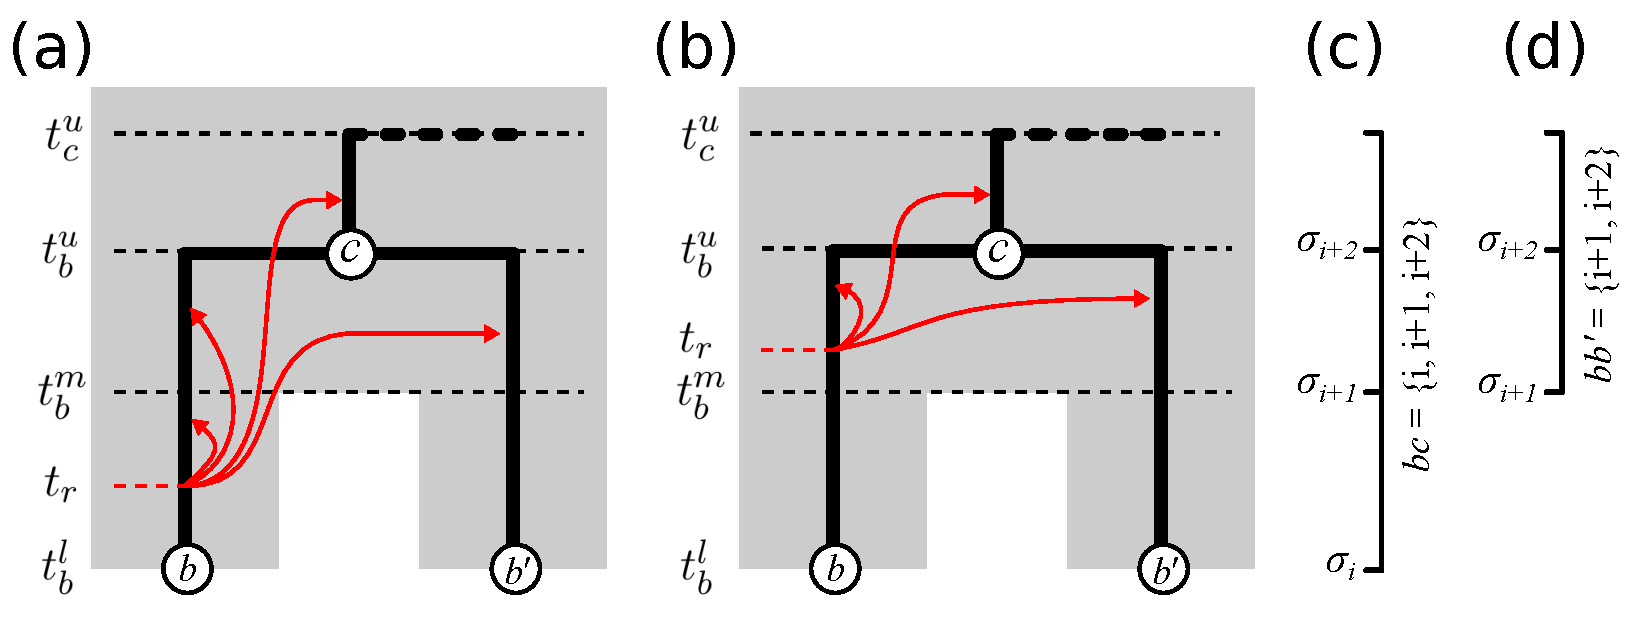
\includegraphics[width=0.75\textwidth]{figures/FigS1-sibling-parent-it2.pdf}
% 	\caption{
% 		To calculate the probability that recombination on a genealogy branch
% 		($b$) leads to a topology change involves summing over the probabilities 
% 		that a detached lineage does not re-coalesce with either
% 		itself ($b$), its sibling ($b'$) or its parent ($c$) branches. At the time 
% 		recombination occurs ($t_r$) the branches $b$ and $b'$ can either exist 
% 		in different species tree intervals (a) or the same interval (b). This 
% 		restricts the probability of tree-change outcomes (e.g., shortened coalescent 
% 		time) until the lowest shared interval between $b$ and $b'$ at time 
% 		$t_m$. This leads to two ordered sets of intervals (c-d) used in 
% 		equations 11 and 12.
% 	}
% 	\label{fig:figSSS}
% \end{figure}



\paragraph{First case --} Given $t_r$ $<$ $t_b^m$, we integrate over the three
distinct intervals where re-coalescence can occur. The first is unique to branch $b$, 
the second integral is multiplied by two since from $t_b^m$ to $t_b^u$ re-coalescence
can occur with $b$ or $b'$, and the final integral is over the length of branch $c$.
By substituting the piece-wise constant solutions for each interval into this equation
it can \textcolor{red}{be} simplifed to the final form below, also shown in equation 11 of the main text:

\begin{equation}
\begin{aligned}
	&\mathbb{P}(\text{topology-unchanged} | \mathcal{S}, \mathcal{G}, b, t_r) \\
	&= \int_{t_r}^{t_b^m}
	\frac{1}{\mathcal{K}(b,\tau)} f(\tau - t_r; \lambda) d\tau + 
	\int_{t_b^m}^{t_b^u}
	\frac{2}{\mathcal{K}(b,\tau)} f(\tau - t_r; \lambda) d\tau + 
	\int_{t_b^u}^{t_c^u} \frac{1}{\mathcal{K}(b,\tau)} f(\tau - t_r; \lambda) d\tau \\
	&= \frac{1}{k_i} + 
	\sum_{j \in \mathcal{I}_{bc}}	f(i,j) \exp \bigg\{	\frac{k_i}{2n_i} t_r \bigg\} + 
	\sum_{j \in \mathcal{M}_b}    f(i,j) \exp \bigg\{ \frac{k_i}{2n_i} t_r \bigg\}
\end{aligned}
\end{equation}

\paragraph{Second case --} Given $t_r$ $>=$ $t_b^m$, we only need to integrate over
two distinct intervals, thus we simply drop the first term from the equation above.
The final form of this equation is also shown in equation 11 of the main text:

\begin{equation}
\begin{aligned}
	&\mathbb{P}(\text{topology-unchanged} | \mathcal{S}, \mathcal{G}, b, t_r) \\
	&= \int_{t_r}^{t_b^u} \frac{2}{\mathcal{K}(b,\tau)} f(\tau - t_r; \lambda) d\tau + 
	 \int_{t_b^u}^{t_c^u} \frac{1}{\mathcal{K}(b, \tau)} f(\tau - t_r; \lambda) d\tau \\
	&= 2 \bigg(
		\frac{1}{k_i} + 
		\sum_{j \in \mathcal{I}_b} f(i,j) \exp \bigg\{ \frac{k_i}{2n_i} t_r \bigg\}
	\bigg) + 
	\sum_{j \in \mathcal{I}_c} f(i,j) \exp \bigg\{ \frac{k_i}{2n_i} t_r \bigg\}
\end{aligned}
\end{equation}

\subsubsection{Across a full branch}

Now we derive the overall probability that a recombination event falling on a specific branch will 
\textcolor{red}{not} change the topology by integrating across the range of possible values for $t_r$.
Following the approach above, we split this problem into two parts, above and below
$t_b^m$, and we sum the two cases.

\begin{equation}
	\mathbb{P}(\text{topology-unchanged} | \mathcal{S}, \mathcal{G}, b) = 
	\frac{1}{t_b^u - t_b^l} \int_{t_b^l}^{t_b^u}
	\mathbb{P}(\text{topology-unchanged} | \mathcal{S}, \mathcal{G},b, t_r) dt_r
\end{equation}

\begin{equation}
	= \frac{1}{t_b^u - t_b^l}
	\bigg[
		\bigg(
			\int_{t_b^l}^{t_b^m} + 
			\int_{t_b^m}^{t_b^u}
		\bigg)
		\mathbb{P}(\text{topology-unchanged} | \mathcal{S}, \mathcal{G},b, t_r) dt_r
	\bigg]
\end{equation}


\paragraph{First case --}
We can simply sum over each entire interval below $t_b^m$ where $t_r$ could occur, and 
substitute piece-wise constant solutions for the probabilities that a detached
subtree will re-coalesce over the subset of targeted intervals above this that
do not cause a topology-change.

\begin{equation}
\begin{aligned}
	&\int_{t_b^l}^{t_b^m} {\mathbb{P}(\text{topology-unchanged} | \mathcal{S}, \mathcal{G}, b, t_r)} dt_r \\
	&= \sum_{i \in \mathcal{L}_b} \frac{1}{k_i} \Bigg[ 
		d_i + 2n_i \bigg( 
			\exp \bigg\{\frac{k_i}{2n_i} \mu_i \bigg\} - 
			\exp \bigg\{\frac{k_i}{2n_i} \sigma_i\bigg\} 
		\bigg)
		\bigg(
			\sum_{j \in \mathcal{I}_{bc}} f(i,j) + \sum_{j \in \mathcal{M}_b} f(i,j) 
		\bigg) 
	\Bigg]
\end{aligned}
\end{equation}

\paragraph{Second case --}
Similarly, we can sum over each entire interval above $t_b^m$ (up to $t_b^u$) and substitute piece-wise
constant solutions for the same selected subset of intervals:

\begin{equation}
\begin{aligned}
	&\int_{t_b^m}^{t_b^u} \mathbb{P} (\textrm{topology-unchanged} | \mathcal{S}, \mathcal{G}, b, t_r) dt_r \\
	&= \sum_{i \in \mathcal{M}_b} \frac{1}{k_i} \Bigg[ 
		2d_i + 2n_i \bigg( 
			\exp \bigg\{ \frac{k_i}{2n_i} \mu_i \bigg\} - 
			\exp \bigg\{ \frac{k_i}{2n_i} \sigma_i \bigg\}
		\bigg) 
		\bigg(2 \sum_{j \in \mathcal{I}_b} f(i,j) + \sum_{j \in \mathcal{I}_c} f(i,j) \bigg)
	\Bigg]
\end{aligned}
\end{equation}

\paragraph{Result --}
If we express the inner summed terms from the equations above, composed of piece-wise
constant values from their intervals, as $p_{b,1}^{(i)}$ and $p_{b,2}^{(i)}$, 
respectively, then the final solution can be expressed more concisely. 
This is shown in the main text as equation 12.

\begin{equation}\tag{12}
     \mathbb{P}(\text{topology-unchanged} | \mathcal{S}, \mathcal{G}, b) = 
     \frac{1}{t_b^u - t_b^l} 
     \bigg[ 
	    \sum_{i \in \mathcal{L}_b} p_{b,1}^{(i)} + 
	    \sum_{i \in \mathcal{M}_b} p_{b,2}^{(i)}
	\bigg]
\end{equation}


\subsubsection{Across the whole tree}

Finally, we sum across all branches, each weighted by their relative length, 
to find the probability of a recombination event \textcolor{red}{not} changing the 
topology of the tree. This appears as equation 13 in the main text.

\begin{equation}\tag{13}
\begin{aligned}
    &\mathbb{P}(\text{topology-unchanged}| \mathcal{S}, \mathcal{G}) = 
    \sum_{b \in \mathcal{G}}
    \frac{t_b^u - t_b^l}
    {L(\mathcal{G})} \times \mathbb{P}(\text{topology-unchanged}| \mathcal{S}, \mathcal{G}, b) \\
    % 
    & = \frac{1}{L(\mathcal{G})} \sum_{b \in \mathcal{G}}
     \bigg[ 
	    \sum_{i \in \mathcal{L}_b} p_{b,1}^{(i)} + 
	    \sum_{i \in \mathcal{M}_b} p_{b,2}^{(i)}
	\bigg]
\end{aligned}
\end{equation}


\subsubsection{Examples}
Examples showing how to compute the \textcolor{red}{probability}\sout{probablity} of a no-change (tree-unchanged) 
or topology-\textcolor{red}{unchanged}\sout{change} event are shown with didactic step-by-step instructions in 
Fig.~\ref{fig:figS-tree-equations} and Fig.~\ref{fig:figS-topo-equations}, 
respectively.



% \begin{figure}[t]
% 	\centering
% 	%\fbox{\rule[-.5cm]{4cm}{4cm} \rule[-.5cm]{4cm}{0cm}}
% 	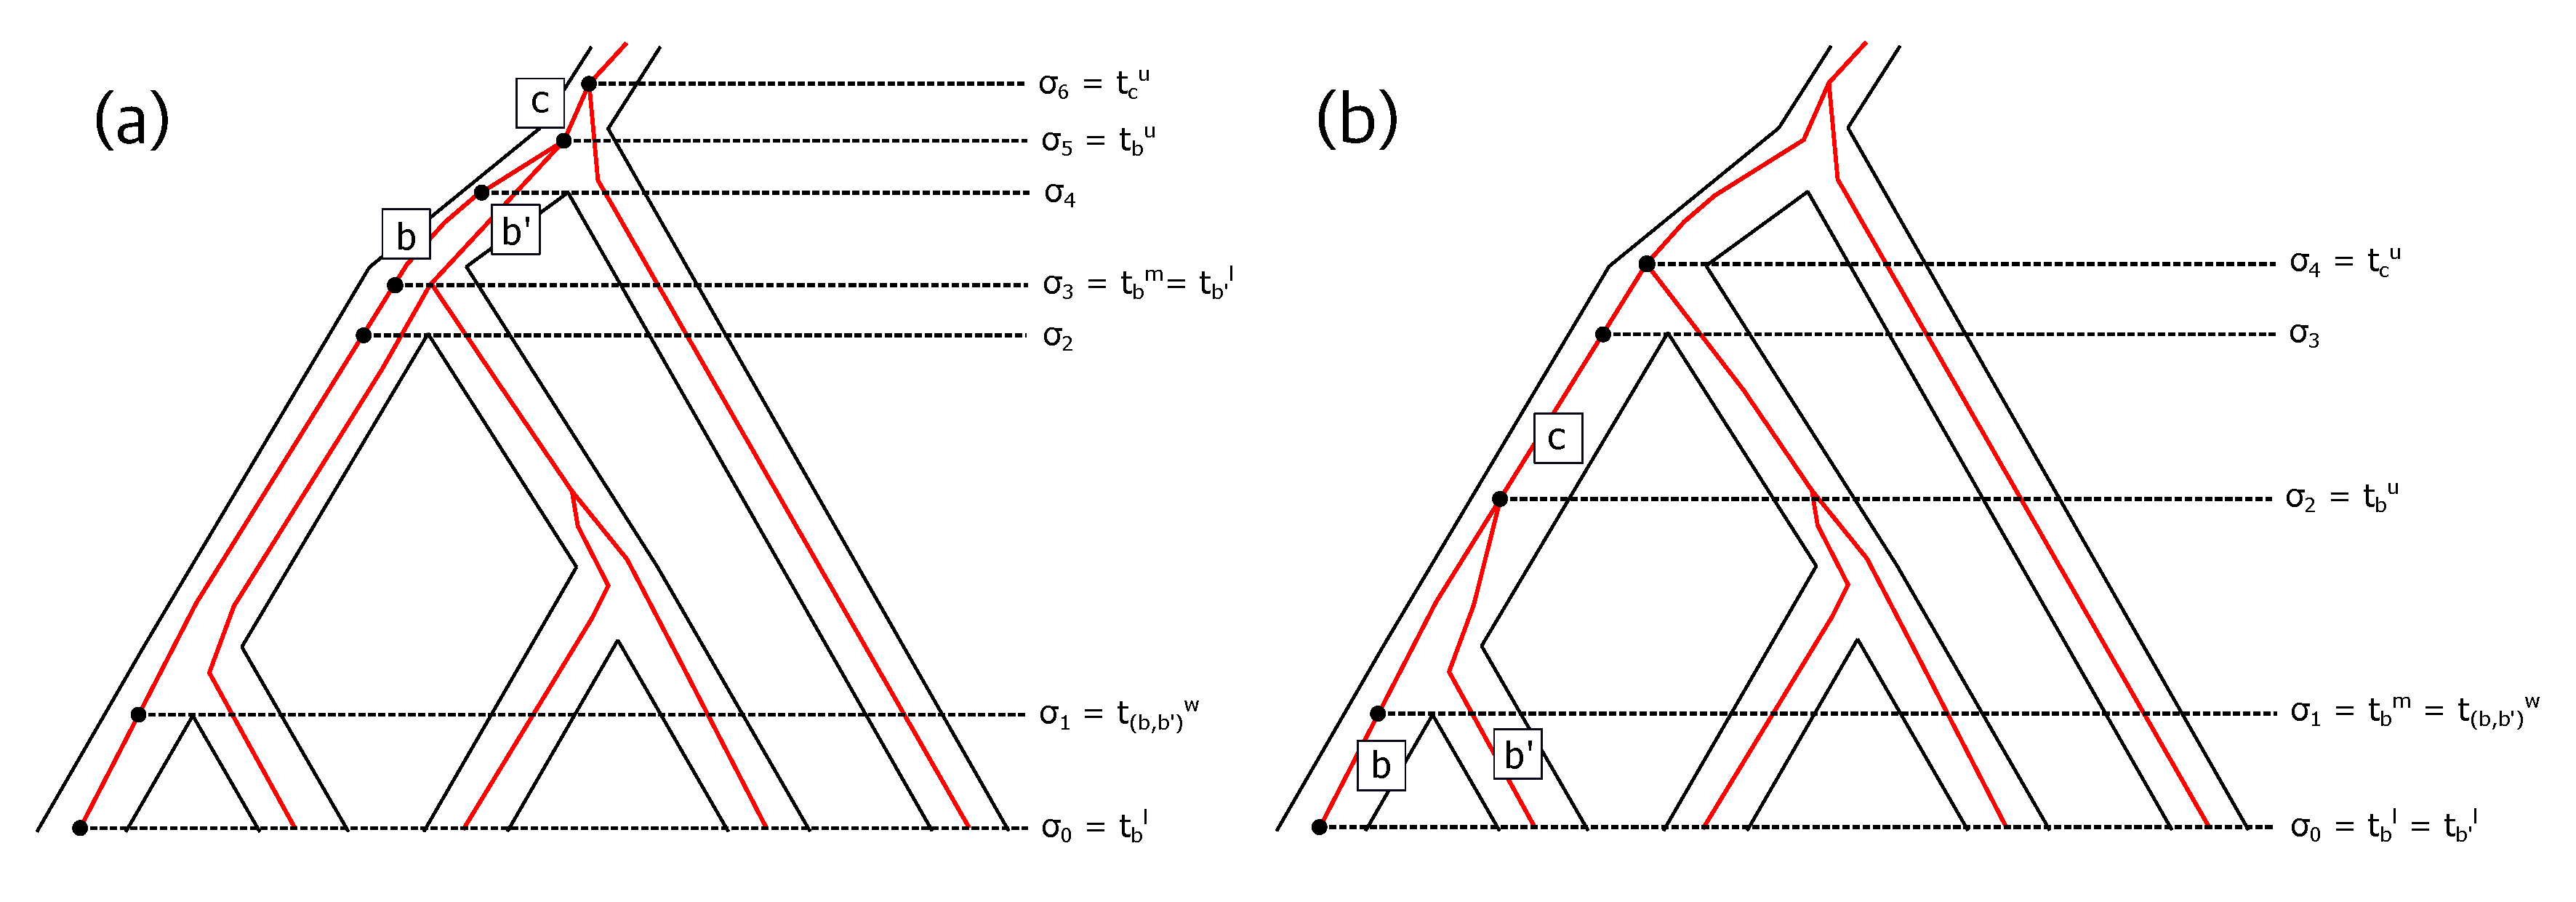
\includegraphics[width=0.9\textwidth]{figures/FigS1-topology_illustration.pdf}
% 	\caption{Illustrating the parameters for calculating the distribution of distances 
% 	to a change in the topology of a genealogy. Panels (a) and (b) show slightly 
% 	different genealogies embedded in the same species tree. In both (a) and (b), 
% 	the focal branch $b$ is the one leading from the left-most species. 
% 	Branches $c$ and $b'$ -- the parent and sibling branches, respectively -- are 
% 	also both labeled. Note that in (a), $t_b^m$ corresponds to $\sigma_3$, while
% 	in (b) it corresponds to $\sigma_1$.}
% 	% \label{fig:fig5}
% \end{figure}


%%%%%%%%%%%%%%%%%%%%%%% This table doesn't seem necessary.
% \begin{table}[h]
% \centering
% \caption{\label{tab:table-S1} 
% 	A table summarizing the relationships among branches in the genealogical tree embedded in the species tree in Figure 1. 
% }
% \begin{tabular}[t]{ |c|c|c|c|c|c|c| }
% 	\toprule
% 	Branch & $\mathcal{I}_b$ & $t_b^l$ & $t_b^u$ & Parent & Sibling & $t_b^m$ \\
% 	\midrule
% 	0  &  1 & 0      & $t_7$  & 7  & 1  & 0          \\
% 	1  &  1 & 0      & $t_7$  & 7  & 0  & 0          \\
% 	2  &  3 & 0      & $t_9$  & 9  & 8  & $W_{AB}$   \\
% 	3  &  1 & 0      & $t_8$  & 8  & 4  & 0          \\
% 	4  &  1 & 0      & $t_8$  & 8  & 3  & 0          \\
% 	5  &  4 & 0      & $t_{11}$ & 11 & 6  & $W_{ABCD}$ \\
% 	6  &  2 & 0      & $t_{11}$ & 11 & 5  & $W_{ABCD}$ \\
% 	7  &  4 & $t_7$  & $t_{10}$ & 10 & 9  & $t_9$      \\
% 	8  &  2 & $t_8$  & $t_9$  & 9  & 2  & $W_{AB}$   \\
% 	9  &  2 & $t_9$  & $t_{10}$ & 10 & 7  & $t_9$      \\
% 	10 &  3 & $t_{10}$ & $t_{12}$ & 12 & 11 & $t_{11}$     \\
% 	11 &  1 & $t_{11}$ & $t_{12}$ & 12 & 10 & $t_{11}$     \\
% 	\bottomrule
% \end{tabular}
% \end{table}





\end{document}
